\documentclass{book}
\usepackage[top=2cm,bottom=2cm,left=2cm,right=2cm]{geometry}
\usepackage{graphicx}
\usepackage{amsmath,amssymb,amsthm}
\usepackage{xkeyval,paralist}
\usepackage{bm} %% bold face math symbols
\usepackage{listings}
\usepackage{tikz}
%\usetikzlibrary{shapes}
\usetikzlibrary{arrows}

\usepackage{stmaryrd}\newcommand{\contra}{\lightning}

\usepackage{rotating} \newcommand{\sw}[1]{\begin{sideways}#1\end{sideways}}

\usepackage{ded}

\usepackage{../mylecturenotes}

\renewcommand{\P}[2]{\Pi #1:#2.}

\usepackage[bookmarks=true, linkcolor=blue, citecolor=blue, urlcolor=blue, colorlinks=true, breaklinks=true, bookmarksopen=true,bookmarksopenlevel=1,bookmarksnumbered]{hyperref} % this needs to go last

\title{Integrated Lectures Notes on Logic}
\author{Florian Rabe}
\date{2008-2016}

\begin{document}
\maketitle

\tableofcontents
\newpage

This is a collection of notes from my undergraduate and graduate lectures on logic.

Standard textbooks for logic are \cite{fol_gallier}, \cite{fol_smullyan}, and \cite{intrologicenderton} (look for the respective latest edition).
\cite{andrews_truthproof} is an interesting textbook that emphasizes higher-order logic and proof theory.

\part{First-Order Logic}\label{part:fol}

\chapter{Syntax}\label{sec:syn}
  \section{Syntax of Propositional Logic}

\begin{definition}[PL-signatures]
A PL-signature is an alphabet, i.e., a set $\Sigma$ of symbols.
\end{definition}

\begin{definition}[PL formulas]
The PL-grammar for the signature $\Sigma$ is:

\begin{tabular}{lcl@{\tb}l}
$\FORM$ & $::=$ & $\true$ & \emph{truth} \\
     &  $|$  & $\false$ & \emph{falsity} \\
     &  $|$  & $\FORM \wedge \FORM$ & \emph{conjunction} \\
     &  $|$  & $\FORM \vee \FORM$ & \emph{disjunction} \\
     &  $|$  & $\FORM \arr \FORM$ & \emph{implication} \\
     &  $|$  & $\neg \FORM$ & \emph{negation} \\
     &  $|$  & $p$ where $p\in\Sigma$ & \emph{boolean variables}\\
\end{tabular}

The set of words over this grammar is the set $\Sen^{PL}(\Sigma)$ of $\Sigma$-\emph{formulas} (also called $\Sigma$-\emph{propositions} or $\Sigma$-\emph{sentences}).
\end{definition}

This grammar is of course ambiguous. If we actually want to parse words, we have to make it unambiguous by adding brackets around conjunctions, disjunctions, and implications.

\begin{remark}
It is a specialty of propositional logic that all formulas are well-formed, i.e., the well-formed PL-formulas over $\Sigma$ are a context-free language.
Normally, the languages are context-sensitive.
\end{remark}

\section{Syntax of First-Order Logic}

\begin{definition}[FOL-Signatures]\label{def:fol:sig}
A FOL-signature is a triple $(\Sigma_p,\Sigma_f,\arit)$ where $\Sigma_p$ and $\Sigma_f$ are disjoint sets of symbols and $\arit:\Sigma_p\cup\Sigma_f\arr\N$ is a mapping.
\end{definition}

The symbols in $\Sigma_p$ and $\Sigma_f$ are called \emph{predicate symbols} and \emph{function symbols}, respectively. If $\arit(s)=0,1,2,3,4,\ldots$, we say that $s$ is a \emph{nullary}, \emph{unary}, \emph{binary}, \emph{ternary}, $4$-ary, \ldots, symbol.

\begin{figure}[htp]
\begin{center}
\begin{tabular}{lcl@{\tb}l}
$\FORM$ & $::=$ & $\true$ & \emph{truth} \\
        &  $|$  & $\false$ & \emph{falsity} \\
        &  $|$  & $\FORM \wedge \FORM$ & \emph{conjunction} \\
        &  $|$  & $\FORM \vee \FORM$ & \emph{disjunction} \\
        &  $|$  & $\FORM \arr \FORM$ & \emph{implication} \\
        &  $|$  & $\neg \FORM$ & \emph{negation} \\
        &  $|$  & $\forall \VAR\; \FORM$ & \emph{universal quantification} \\
        &  $|$  & $\exists \VAR\; \FORM$ & \emph{existential quantification} \\
        &  $|$  & $p(\underbrace{\TERM,\ldots,\TERM}_n)$ where $p\in\Sigma_p$ with $\arit(p)=n$ & \emph{atomic formulas} or \emph{predicates}\\
$\TERM$ & $::=$ & $f(\underbrace{\TERM,\ldots,\TERM}_n)$ where $f\in\Sigma_f$ with $\arit(f)=n$ \\
        &  $|$  & $\VAR$ &\\
$\VAR$  & $::=$ & some symbol & \emph{variables}
\end{tabular}
\caption{FOL Grammar}\label{fig:fol:grammar}
\end{center}
\end{figure}

\begin{definition}[FOL-Grammar]\label{def:fol:grammar}
The FOL-grammar for the signature $\Sigma=(\Sigma_p,\Sigma_f,\arit)$ is given by the productions in Fig.~\ref{fig:fol:grammar} with start symbol $\FORM$.

The language of this grammar is denoted by $\Forms^{FOL}(\Sigma)$.
\end{definition}

Words produced from $\TERM$ are called \emph{terms}.
Words produced from $\FORM$ are called \emph{formulas} (or propositions or sentences).

Words produced from $\VAR$ are variable names.
These are elements of some countable set that is usually left implicit.
For example, we can put
\[L(\VAR)=\{x_n,y_n,z_n \| n\in \N\}.\]

This grammar is also ambiguous. To make it unambiguous, we have to add brackets around all complex formulas.

\begin{remark}
The intuition behind the arity is that it gives the number of arguments that a function or predicate symbol takes.

Arity $0$ is permitted: Nullary function symbols are also called \emph{constant} symbols, nullary predicate symbols are the \emph{boolean variables} from propositional logic.
\end{remark}

\begin{remark}
The intuition behind the non-terminals $\TERM$ and $\FORM$ is that terms represent mathematical objects and formulas represent properties of mathematical objects.

It is easy to see that the FOL syntax is an extension of the PL-syntax.

Note that formulas and terms are not mixed: In every branch of the syntax tree of a well-formed formula, all $\FORM$-nodes occur above all $\TERM$-nodes.
\end{remark}

Equality is needed so often that we define FOLEQ. It is like FOL but with a fixed binary predicate symbol $\doteq$ that is always present.

\begin{definition}[FOL with equality]
FOLEQ is defined like FOL but with one production added to the grammar: $\FORM ::= \TERM \doteq \TERM$.
\end{definition}

\begin{remark}[Equality]
It is crucial to understand the difference between $=$ and $\doteq$.

$\doteq$ is a symbol of the alphabet, which happens to look very similar to the symbol $=$.
But at this point $\doteq$ has no meaning whatsoever.
It just takes two term and turns them into a formula.

$=$ on the other hand, has a meaning: It denotes equality of mathematical objects.
In particular, we can use $=$ to express the equality of words over our alphabets, e.g., the equality of terms and formulas.
For example, we can say the following: "We assume $F=s\doteq t$." This sentence expresses that $F$ is a word (in this case a formula) over the alphabet and $F$ is the formula $s\doteq t$.
\end{remark}

\begin{example}[Set Theory]
Axiomatic set theory was introduced around the 1920s by Zermelo and Fraenkel. It is the base of all modern mathematics. In modern language and notation, a very simple variant of axiomatic set theory is based on the following FOLEQ-signature:
\begin{itemize}
\item a binary predicate symbol $\in$, and we usually write $s\in t$ instead of $\in(s,t)$
\item a nullary function symbol $\es$,
\item a unary function symbol $\op{Pow}$,
\item a unary function symbol $\bigcup$,
\item a binary function symbol $\op{unorderedpair}$, and we usually write $\{s,t\}$ instead of $\op{unorderedpair}(s,t)$.
\end{itemize}

Example formulas for this signature are
\begin{itemize}
\item $\forall x \; \neg x\in\es$,
\item $\forall x \; \forall y \; x \in \{x,y\}$,
\item $\forall x \; \forall y \; \{x,y\} \doteq \{y,x\}$,
\item $\forall x \; \es \doteq \{x,x\}$,
\item $\forall x \; \forall y \; x \in y$.
\end{itemize}
Note the difference between the first three and the last two formulas: The first three feel "correct" or "true", whereas the last two feel "false". However, at this point, no formula has a meaning. They are all just words over our grammar.

This signature looks like it has only very few and very boring terms, for example $\es$, $\op{Pow}(\es)$, $\{\es,\es\}$, and so on. And the formulas are even more boring because there is only one predicate symbol. However, together with some abbreviations, this is already enough to talk about most of mathematics.

For example, mathematics usually uses the following abbreviations for terms and formulas:
\begin{itemize}
\item If $s$ and $t$ are terms, then the term $\{s,\{s,t\}\}$ is abbreviated as $(s,t)$.
\item If $s$ and $t$ are terms, then the term $\bigcup\{s,t\}$ is abbreviated as $s\cup t$ (or $(s\cup t)$ if there are ambiguities otherwise).
\item If $s$ is a term, then the term $\{s,s\}$ is abbreviated as $\{s\}$.
\item If $s$ and $t$ are terms (which do not use the variable $x$), then the formula $\forall x\; (x\in s \arr x\in t)$ is abbreviated as $s\sq t$.
\end{itemize}

Then we can give even more abbreviations:
\begin{itemize}
\item We write $0$ instead of $\es$.
\item We write $1$ instead of $\{\es\}$.
\item We write $2$ instead of $\{\es,\{\es\}\}$.
\item We write $3$ instead of $2\cup\{2\}$.
\item and so on
\end{itemize}
\end{example}

\begin{example}[Monoids and Groups]
Monoids and groups (as well as rings, fields, etc.) can also be expressed as FOLEQ signatures.
The signature for monoids has:
\begin{itemize}
\item a binary function symbol $\circ$, and we usually write $s\circ t$ instead of $\circ(s,t)$ (again we may have to write $(s\circ t)$ to prevent ambiguities),
\item a nullary function symbol $e$.
\end{itemize}
The signature for groups extends the signature for monoids with
\begin{itemize}
\item a unary function symbol $\op{inv}$, and we usually write $s^{-1}$ instead of $\op{inv}(s)$.
\end{itemize}
\end{example}


%\section{Induction on Syntax Trees}
%
%We know two induction principles for formal languages:
%\begin{itemize}
%\item Induction on (the length of) the word with
%  \begin{itemize}
%   \item base case: $w=\epsilon$ (i.e., $|w|=0$)
%   \item step case: $w=w'x$ (alternatively: $w=xw'$) for a word $w$ and a symbol $x$ (i.e., $|w|=|w'|+1$)
%  \end{itemize}
%\item Induction on (the length of) the derivation $S\Arr^* w$ with
%  \begin{itemize}
%   \item base case: $S\Arr^* w=S$ (i.e., derivation length $0$)
%   \item step case: $S\Arr^* w' \Arr w$ for a word $w'$ (i.e., derivation length of $S\Arr^* w' \Arr w$ is one plus the derivation length of $S\Arr^* w'$)
%  \end{itemize}
%\end{itemize}
%
%
%Induction on syntax trees is very similar to induction on derivations. Induction on (the height of) the syntax tree with root $S$ and yield $w$ works as follows:
%\begin{itemize}
%   \item base case: $w=S$, then the syntax tree has a single node $S$ and thus height $0$,
%   \item step case: $S\Arr^* A_1\ldots A_n \Arr^* w_1\ldots w_n$ for non-terminals $A_i$ and for all $i$ either $w_i=A_i$ or there is a production $A_i\arr w_i$ in the grammar, then the height of the syntax tree is (at most) one plus the height of the syntax tree with root $S$ and leaves $A_i$.
%\end{itemize}
%The only difference is that in an induction on derivations, we only apply a single production in the induction step, whereas in an induction on syntax trees we can apply several productions at once. Usually, induction on syntax trees is useless because an induction on derivations works as well and is much simpler. However, induction on syntax trees is useful when we do the induction step in the other direction: instead of appending productions at the leaves of the syntax tree, we append one at the root. We call this bottom-up induction on syntax trees.
%
%Bottom-up induction on (the height of) syntax trees with yield $w$ works as follows:
%\begin{itemize}
% \item base case: $w$ is a terminal word produced in a single production from \emph{some} non-terminal symbol (i.e., the height of the syntax tree is $1$),
% \item step case:
%    \begin{itemize}
%      \item if $w_1,\ldots, w_n$ are terminal words such that either $A_i=w_i$ or $w_i$ is the yield of a syntax tree with root $A_i$,
%      \item and if $A\arr A_1\ldots A_n$ is a production of the grammar,
%      \item then the induction step goes from $A_i\Arr^* w_i$ (with height of the syntax trees at most $n$) to $A\Arr A_1\ldots A_n\Arr^* w_1\ldots w_n$ (with height of the syntax tree $n+1)$.
%    \end{itemize}
%\end{itemize}
%Note that because we append productions at the roots of the syntax trees, the non-terminal at the root changes in the induction step. Therefore, we often need different induction steps for different non-terminals at the root.

\section{Contexts and Substitutions}

\paragraph{Free and Bound Variables}
Bottom-up induction on syntax trees is the most important induction for logics and similar languages. It is often just called "induction on the grammar", or ``induction on the language'', or even just ``induction''.
The following definitions are done in this way. The following definitions are for FOLEQ; the analogues for FOL are obtained by deleting the case for $\doteq$.

\begin{definition}[Bound Variables]\label{def:fol:bv}
We define the set $\BV(w)$ of \emph{bound variables} of a word $w$ --- i.e., a formula or a term --- as follows.
\begin{itemize}
  \item for terms:
   \begin{itemize}
    \item $\BV(x)=\es$,
    \item $\BV(f(t_1,\ldots,t_n))=\BV(t_1)\cup\ldots\cup\BV(t_n)$,
   \end{itemize}
  \item for formulas:
   \begin{itemize}
    \item $\BV(p(t_1,\ldots,t_n))=\BV(t_1)\cup\ldots\cup\BV(t_n)$,
    \item $\BV(t_1\doteq t_2)=\BV(t_1)\cup\BV(t_2)$,
    \item $\BV(\true)=\es$,
    \item $\BV(\false)=\es$,
    \item $\BV(F\wedge G)=\BV(F)\cup\BV(G)$ and accordingly for the other connectives,
    \item $\BV(\forall x\;F)=\BV(F)\cup\{x\}$ and accordingly for the other quantifier.
  \end{itemize}
\end{itemize}
\end{definition}

The opposite of bound variables are the free variables.
\begin{definition}[Free Variables]\label{def:fol:fv}
We define the set $\FV(w)$ of \emph{free variables} of a word $w$ --- i.e., a formula or a term --- as follows.
\begin{itemize}
  \item for terms:
   \begin{itemize}
    \item $\FV(x)=\{x\}$,
    \item $\FV(f(t_1,\ldots,t_n))=\FV(t_1)\cup\ldots\cup\FV(t_n)$,
   \end{itemize}
  \item for formulas:
   \begin{itemize}
    \item $\FV(p(t_1,\ldots,t_n))=\FV(t_1)\cup\ldots\cup\FV(t_n)$,
    \item $\FV(t_1\doteq t_2))=\FV(t_1)\cup\FV(t_2)$,
    \item $\FV(\true)=\es$,
    \item $\FV(\false)=\es$,
    \item $\FV(F\wedge G)=\FV(F)\cup\FV(G)$ and accordingly for the other connectives,
    \item $\FV(\forall x\;F)=\FV(F)\sm\{x\}$ and accordingly for the other quantifier.
  \end{itemize}
\end{itemize}
\end{definition}


\begin{remark}
Note that:
\begin{itemize}
\item $x\in\BV(F)$ iff there is a $\forall x$ or a $\exists x$ in $F$. We say that, e.g., $\forall x \; F$ binds the variable $x$ in $F$. $\forall$ and $\exists$ are called \emph{binders}.
\item For a term $t$, we always have $\BV(t)=\es$ because terms cannot contain binders. This is a special property of FOL and FOLEQ  --- for example, lambda calculus is a language where terms may contain binders (namely the $\lambda$ binder).
\item The sets $\FV(F)$ and $\BV(F)$ are always finite.
\item The definitions of $\BV(-)$ and $\FV(-)$ only differ in two cases.
\item If a variable $x$ occurs in $F$, then $x\in\BV(F)$ or $x\in\FV(F)$ or both. For example, $x$ occurs both free and bound in $p(x)\wedge\forall x\;q(x)$.
\end{itemize}
\end{remark}

\begin{remark}
A $\Sigma$-formula/term with an empty set of free variables is called \emph{closed} or a \emph{ground formula/term}.
Ground formulas are often called \emph{sentences} and

If $F$ is a formula with $\FV(F)=\{x_1,\ldots,x_n\}$, then $\forall x_1\;\ldots\;\forall x_n\;F$ and $\exists x_1\;\ldots\;\exists x_n\;F$ are closed formulas. We call them the \emph{universal closure} and the \emph{existential closure} of $F$.
\end{remark}

\begin{example}
Here are some examples for free and bound variables:
\begin{itemize}
\item For the formula $F\;=\; x\circ (y\circ z) \doteq (x\circ y)\circ z$ over the signature of monoids, we have $\BV(F)=\es$ and $\FV(F)=\{x,y,z\}$. Its universal closure is $\forall x\;\forall y\;\forall z\;x\circ (y\circ z) \doteq (x\circ y)\circ z$.
\item There are not so many ground terms over the signature of monoids: They are $e$, $e\circ e$, $(e\circ e)\circ e$, $e\circ(e\circ e)$, and so on.
\item If a FOL- or FOLEQ-signature has no constant symbols, then there are no ground terms.
\item If a FOL-signature has a unary predicate symbol $p$, then $\exists x\;p(x)$ is a (non-boring) ground formula.
\item If a FOLEQ-signature has a unary function symbol $f$, then $\exists x\;x\doteq f(x)$ is a (non-boring) ground formula.
\end{itemize}
\end{example}
The last two examples show that even with only one function or predicate symbol, FOL and FOLEQ already offer a lot of interesting formulas to study.


\paragraph{Contexts}
Above we defined the syntax FOLEQ by using a context-free grammar.
This grammar produced all formulas, i.e., formulas with any number of free variables.
This is often not desirable because we usually only care about closed formulas.

However, the language of closed formulas is not context-free.
This is easy to see: Every binder $\forall x\;F$ declares a variable $x$; this variable is \emph{local} in the sense that it has a certain \emph{scope} and should only occur within its scope; for example, in $G\wedge\forall x\;F$, the scope of $x$ is $F$ (but not $G$).
In general, all languages with such declarations are not context-free.
Therefore, we can only give a context-free grammar for formulas but not for closed formulas.

This is the main reason why we use formulas with free variables at all: We can write down a context-free grammar for them, and such a grammar gives us the powerful and simple induction principle of induction on syntax trees.

In general, we use contexts to keep track of the free variables:

\begin{definition}[Context]\label{def:fol:context}
Let $\Sigma$ be a signature.
A $\Sigma$-\emph{context} $\Gamma$ is a finite set of variables.

We define
\[\isformSG{F} \tb\miff\tb F\in \Forms^{FOLEQ}(\Sigma) \mand \FV(F)\sq\Gamma\]
If $\isformSG{F}$, we say that $F$ is a $\Sigma$-formula in context $\Gamma$.
If $\Gamma=\es$, we write $\isform{\Sigma}{}{F}$.

Finally, we define
\[\Sen^{FOLEQ}(\Sigma)=\{F \,|\,\isform{\Sigma}{}{F}\}\]
\end{definition}


\begin{example}
Let $\Sigma$ be the signature of monoids.
The formula $x\circ (y\circ z) \doteq (x\circ y)\circ z$ is a formula in the context $\{x,y,z\}$:
\[\isformS{x,y,z}{x\circ (y\circ z) \doteq (x\circ y)\circ z}\]
It is also a formula in any bigger context:
\[\isformS{x,x',y,z,y'}{x\circ (y\circ z) \doteq (x\circ y)\circ z}\]
\end{example}

\paragraph{Substitutions}
We can think of free variables as holes or placeholder that can be filled with arbitrary terms.
This filling operation is the task of substitutions.

\begin{definition}[Substitution]\label{def:fol:sub}
Let $\Sigma$ be a signature. A \emph{substitution} from a $\Sigma$-context $\Gamma$ to a $\Sigma$-context $\Gamma'$ is a mapping from $\Gamma$ to $\Sigma$-terms in context $\Gamma'$.
\end{definition}

\begin{notation}
If $\gamma$ is a substitution from $\Gamma$ to $\Gamma'$, we write $\gamma:\Gamma\arr\Gamma'$.
If $\Gamma=\{x_1,\ldots,x_n\}$ and $\gamma(x_i)=t_i$, we write $\gamma$ as $[\sub{x_1}{t_1},\ldots,\sub{x_n}{t_n}]$.
\end{notation}

\begin{remark}[Contexts]
It is not so common to use contexts when talking about FOL and FOLEQ. When you study additional literature, you will probably not find them. The reason is that --- contrary to other logics --- FOL and FOLEQ are so simple that contexts are not needed. However, contexts make a lot of things much clearer and more elegant, and a good computer scientist should understand them.
\end{remark}

\begin{notation}
Some literature writes substitutions the other way around: $\sub{t}{x}$ instead of $\sub{x}{t}$.
\end{notation}

\begin{example}\label{ex:fol:sub}
Let $\Sigma$ be the signature of monoids.
\begin{itemize}
\item If $\Gamma=\{x,y,z\}$ and $\Gamma'=\{x,u,v,y\}$, then $[\sub{x}{y},\sub{y}{x},\sub{z}{e\circ v}]$ is a substitution from $\Gamma$ to $\Gamma'$.
\item The identity $[\sub{x_1}{x_1},\ldots,\sub{x_n}{x_n}]$ is a substitution from the context $\{x_1,\ldots,x_n\}$ to itself.
\item More generally, $[\sub{x_1}{x_1},\ldots,\sub{x_n}{x_n}]$ is a substitution from the context $\{x_1,\ldots,x_n\}$ to any context $\Gamma'$ with $\{x_1,\ldots,x_n\}\sq\Gamma'$.
\end{itemize}
\end{example}

The intuition behind a substitution $[\sub{x_1}{t_1},\ldots,\sub{x_n}{t_n}]$ from $\Gamma$ to $\Gamma'$ is that every (free) variable $x_i$ occurring in a formula/term over $\Gamma$ is substituted with $t_i$ thus creating a formula/term over $\Gamma'$. This is formalized in the following definition.

\begin{definition}[Substitution application]\label{def:fol:subapp}
Let $\Sigma$ be a signature and $\gamma:\Gamma\arr\Gamma'$ a substitution between $\Sigma$-contexts. Then we define the \emph{application} $\ov{\gamma}(-)$ of $\gamma$ to a word as follows:
\begin{itemize}
\item terms:
  \begin{itemize}
    \item $\ov{\gamma}(x)=\gamma(x)$,
     \item $\ov{\gamma}(f(t_1,\ldots,t_n))=f\big(\ov{\gamma}(t_1),\ldots,\ov{\gamma}(t_n)\big)$,
  \end{itemize}
\item formulas:
   \begin{itemize}
     \item $\ov{\gamma}(p(t_1,\ldots,t_n))=p\big(\ov{\gamma}(t_1),\ldots,\ov{\gamma}(t_n)\big)$,
     \item $\ov{\gamma}(t_1\doteq t_2)=\ov{\gamma}(t_1)\doteq\ov{\gamma}(t_2)$,
     \item $\ov{\gamma}(\true)=\true$,
     \item $\ov{\gamma}(\false)=\false$,
     \item $\ov{\gamma}(F\wedge G)=\ov{\gamma}(F)\wedge\ov{\gamma}(G)$ and similarly for the other connectives,
     \item $\ov{\gamma}(\forall x\;F)=\forall x\;\ov{\gamma^x}(F)$ and similarly for the other quantifier.
   \end{itemize}
   Here $\gamma^x$ is a substitution from $\Gamma\cup\{x\}$ to $\Gamma'\cup\{x\}$ defined by $\gamma^x(x)=x$ and $\gamma^x(y)=\gamma(y)$ for all variables $y$ in $\Gamma$. (In the special case where $x\in\Gamma$, the former takes precedence.)
\end{itemize}
\end{definition}

\begin{notation}\label{not:fol:sub}
If $F$ is a formula with $\FV(F)=x_1,\ldots,x_n$, it is common to use the following abbreviation:
\[F(t_1,\ldots,t_n) \tb := \tb \ov{[\sub{x_1}{t_1},\ldots,\sub{x_n}{t_n}]}(F).\]
And similarly, if $t$ is a term with $\FV(t)=x_1,\ldots,x_n$, then:
\[t(t_1,\ldots,t_n) \tb := \tb \ov{[\sub{x_1}{t_1},\ldots,\sub{x_n}{t_n}]}(t).\]

Moreover, we use the following abbreviations
\[F[\sub{x_1}{t_1},\ldots,\sub{x_n}{t_n}] \tb := \tb \ov{[\sub{x_1}{t_1},\ldots,\sub{x_n}{t_n}]}(F).\]
\[t[\sub{x_1}{t_1},\ldots,\sub{x_n}{t_n}] \tb := \tb \ov{[\sub{x_1}{t_1},\ldots,\sub{x_n}{t_n}]}(t).\]
\end{notation}

There is one tricky problem with substitutions. Assume $\gamma=[\sub{x}{y}]:\{x\}\arr\{y\}$. Then $\ov{\gamma}(\forall y\;p(x,y))=\forall y\;p(y,y)$. This is not intended: We want to obtain something like $\forall y'\;p(y,y')$, i.e., we want to distinguish the first $y$, which should stem from the context $\{y\}$ and the second one, which should stem from the binder $\forall y$. If a substitution makes two variables equal that are supposed to different, we speak of \emph{variable capture}. In this example, we can avoid variable capture only by renaming $y$ to $y'$. This is called $\alpha$-\emph{renaming}.

\begin{definition}[$\alpha$-renaming]
Replacing a (sub-)formula $\forall x\;F$ with $\forall x'\;F'$ where $F'$ is like $F$ but with all occurrences of $x$ replaced with $x'$ is called an $\alpha$-\emph{renaming} (from $x$ to $x'$). The same holds for $\exists$ instead of $\forall$.
\end{definition}

More generally, we can always avoid variable capture as follows: Before applying the substitution $\gamma:\Gamma\arr\Gamma'$ to the formula $F$, we use $\alpha$-renaming to replace all variables $x\in\BV(F)\cap\Gamma'$ with other variables. If we want to indicate that we do that, we speak of \emph{capture-avoiding substitutions}.

\begin{example}\label{ex:fol:subapp}
Let $\Sigma$ be the signature of monoids. Let $\Gamma=\{x,y,z\}$ and $\Gamma'=\{x,u,v,y\}$, and $\gamma=[\sub{x}{y},\sub{y}{x},\sub{z}{e\circ v}]$ as above. Then
\begin{itemize}
\item $\ov{\gamma}\big(x\circ (y\circ z) \doteq (x\circ y)\circ z\big) \tb=\tb y\circ (x\circ (e\circ v)) \doteq (y\circ x)\circ (e\circ v)$,
\item $\ov{\gamma}\big(\forall z \; x\circ (y\circ z) \doteq (x\circ y)\circ z\big) \tb=\tb \forall z \; y\circ (x\circ z) \doteq (y\circ x)\circ z$,
\item $\ov{\gamma}\big(\forall y \; x\circ (y\circ z) \doteq (x\circ y)\circ z\big) \tb=\tb
                       \forall y \; y\circ (y\circ (e\circ v)) \doteq (y\circ y)\circ (e\circ v)$ 
                       \\ (variable capture)
\item $\ov{\gamma}\big(\forall y' \; x\circ (y'\circ z) \doteq (x\circ y')\circ z\big) \tb=\tb
                       \forall y' \; y\circ (y'\circ (e\circ v)) \doteq (y\circ y')\circ (e\circ v)$
                       \\ (capture-avoiding variant of the above after $\alpha$-renaming of $y$ to $y'$)
\end{itemize}
\end{example}

Eventually we can state the main property of substitutions:
\begin{theorem}[Closure under Substitution]
Let $\Sigma$ be a signature and $\gamma:\Gamma\arr\Gamma'$ a substitution between $\Sigma$-contexts. Then:
\begin{itemize}
\item if $\istermSG{t}$, then $\istermS{\Gamma'}{\ov{\gamma}(t)}$,
\item if $\isformSG{F}$, then $\isformS{\Gamma'}{\ov{\gamma}(F)}$,
\end{itemize}
where, if necessary, the substitution application uses $\alpha$-renaming in $F$ such that variable capture is avoided.
\end{theorem}
\begin{proof}
This is left as an exercise.
\end{proof}

\section{An Abstract Definition of the Syntax of a Logic}\label{sec:syn:abs}

Above we have seen the signatures and formulas of three logics: PL, FOL, and FOLEQ. And there are many more logics: Researchers have developed all kinds of logics for different purposes. For example, two general ways how to obtain new logics from old ones are the following.
\begin{itemize}
\item Changing the signatures: for example, ALGEQ (algebraic equational logic) arises from FOLEQ by only using signatures without predicate symbols.
\item Changing the formulas: for example, HORNEQ (equational Horn logic) arises from FOLEQ by only allowing formulas that look like this:
\[\forall x_1 \ldots \forall x_m\; ((F_1\wedge \ldots \wedge F_n) \arr F)\]
where all the $F_1,\ldots,F_n,F$ are atomic (i.e., they do not contain proper subformulas).
\end{itemize}

Therefore, it is important to study the abstract properties of logics so that we can work with all these logics at once. Otherwise, every definition or theorem would have to be repeated for every logic.

Therefore, we introduce the following definition.

\begin{definition}\label{def:syn:abs}
A \emph{logic syntax} is a pair $(\Sig,\Sen)$ where $\Sig$ is a collection of objects --- called the \emph{signatures} --- and $\Sen$ is a mapping from $\Sig$ to sets, i.e., if $\Sigma\in\Sig$, then $\Sen(\Sigma)$ is a set. The elements of $\Sen(\Sigma)$ are called the $\Sigma$-\emph{sentences}.
\end{definition}

\begin{example}\label{ex:syn:abs}
Now we can say:
\begin{itemize}
\item Let $\Sig^{PL}$ be the collection of PL-signatures, and $\Sen^{PL}$ be the mapping that maps a PL-signature to its set of PL-formulas. Then $(\Sig^{PL},\Sen^{PL})$ is a logic syntax.
\item Let $\Sig^{FOL}$ be the collection of FOL-signatures, and $\Sen^{FOL}$ be the mapping that maps a FOL-signature to its set of FOL-sentences. Then $(\Sig^{FOL},\Sen^{FOL})$ is a logic syntax.
\item The logic syntax $(\Sig^{FOLEQ},\Sen^{FOLEQ})$ is defined similarly to $(\Sig^{FOL},\Sen^{FOL})$.
\end{itemize}
\end{example}
\medskip

When defining logics (or related formalisms) in this way, we typically end up with the following situation:
\begin{itemize}
\item There is a collection of signatures $\Sigma$.
\item For every signature, there is a collection of contexts $\Con(\Sigma)$.
\item For every signature $\Sigma$ and every context $\Gamma$, there is the set of formulas $\isformSG{F}$.
\item For a fixed signature $\Sigma$, we can use substitutions $\gamma:\Gamma\arr\Gamma'$ between two $\Sigma$-contexts $\Gamma$ and $\Gamma'$.
\item Such a substitution $\gamma:\Gamma\arr\Gamma'$ induces a mapping from formulas $\isformSG{F}$ to formulas $\isformS{\Gamma'}{\ov{\gamma}(F)}$.
\end{itemize}
For example, this is the case for FOL and FOLEQ. FOL and FOLEQ have the special property that for all signatures $\Sigma$, the contexts are simply finite sets of variables. In other logics, the contexts can be more complex.


\section{Theories}\label{sec:fol:thysyn}

The above definition of logic syntax comes in very handy when we define theories: Theories are defined in exactly the same way for every logic. With our definition of logic syntax, we can handle all logics at once.

\begin{definition}[Theories]
Let $L=(\Sig,\Sen)$ be a logic syntax. Then an $L$-\emph{theory} is pair $(\Sigma,\Theta)$ where $\Sigma\in\Sig$ and $\Theta\sq\Sen(\Sigma)$. The formulas in $\Theta$ are called the \emph{axioms} of the theory.
\end{definition}

The most important logic, for which theories are used, is FOLEQ. A FOLEQ-theory is a pair of a FOLEQ signature and a set of FOLEQ-formulas. Let us look at some examples of FOLEQ-theories.\medskip

\begin{example}[Set Theory]\label{ex:set}
Below we will use the abbreviation $F\darr G$ for $(F\arr G)\wedge (G\arr F)$.
The theory of set theory consists of the above-mentioned signature for set theory and the following axioms:
\begin{itemize}
\item axiom of equality (also called extensionality, intuitively: Two sets are equal if they have the same elements.): $\forall X\;\forall Y\;(X\doteq Y \darr \forall z\;(z\in X \darr z \in Y))$,
\item axiom characterizing the empty set: $\forall x\; \neg x\in\es$,
\item axioms characterizing the unordered pair: $\forall x\;\forall y\;\{x,y\}\doteq\{y,x\}$ and $\forall x\;\forall y\;x\in\{x,y\}$,
\item axiom characterizing the union: $\forall X\;\forall z\; (z\in\bigcup X \darr \exists x\;(x \in X \wedge z\in x))$,
\item axiom characterizing the power set: $\forall X\;\forall z\; (z\in \op{Pow}(X) \darr z \sq X)$,
\item some other axioms, which would go beyond the scope of this lecture. A nice overview is given at \url{http://en.wikipedia.org/wiki/Zermelo\%E2\%80\%93Fraenkel_set_theory}. However, there the variant of set theory is used where $\in$ is the only function/predicate symbol.
\end{itemize}
As said above, this formulation of set theory goes back to works by Zermelo and Fraenkel in the 1920s \cite{zermelo,fraenkel}.
However, it was not originally written in FOLEQ.
In fact, FOLEQ was not even fully understood yet at the time.
It has undergone various changes in modern mathematics, and today different versions of set theory are used.
\end{example}

\begin{example}[Monoids]\label{ex:monoid}
The theory of monoids consists of the above-mentioned signature for monoids and the following axioms:
\begin{itemize}
\item associativity: $\forall x\;\forall y\;\forall z\;x\circ (y\circ z) \doteq (x\circ y)\circ z$,
\item left-neutrality: $\forall x\;e\circ x \doteq x$,
\item right-neutrality: $\forall x\;x\circ e \doteq x$.
\end{itemize}
\end{example}

\begin{example}[Groups]\label{ex:group}
The theory of groups consists of the above-mentioned signature for groups, all the axioms of the theory of monoids, and the following axioms:
\begin{itemize}
\item left-inverseness: $\forall x\;x\circ x^{-1} \doteq e$,
\item right-inverseness: $\forall x\;x^{-1}\circ x \doteq e$.
\end{itemize}
\end{example}

\begin{example}[Natural numbers]\label{ex:nat:succ}
The theory of natural numbers is a tricky one, which we will come back to later (see Ex.~\ref{ex:nat:incomplete} and~\ref{ex:nat:fol:induction}). For now we can define it like this:
\begin{itemize}
\item a nullary function symbol $0$,
\item a unary function symbol $\op{succ}$,
\item an axiom for the injectivity of $\op{succ}$: $\forall x\;\forall y\;(\op{succ}(x)\doteq\op{succ}(y)\arr x\doteq y)$,
\item an axiom that makes $0$ the starting point: $\neg\exists x\;0\doteq\op{succ}(x)$.
\item a set of axioms for induction: For every formula $F$ with $\FV(F)=\{x\}$, the axiom
 \[\big(F(0) \wedge \forall\;x \big(F(x)\arr F(\op{succ}(x))\big)\big)\arr\forall x\; F(x).\]
\end{itemize}
These are Peano's axioms from 1889 \cite{peanoaxioms}. As for set theory, they were written at a time when researchers only began to study the notions of logic and formal syntax. In particular, Peano did not know FOLEQ as we do today.
\end{example}

\begin{example}[Natural numbers]\label{ex:nat:arith}
A variant of the theory of natural numbers -- usually called Peano arithmetic -- extends Ex.~\ref{ex:nat:succ} with:
\begin{itemize}
\item binary function symbols $+$ and $\cdot$,
\item two axioms that define addition inductively,
\item two axioms that define multiplication inductively.
\end{itemize}
\end{example}



  
\chapter{Context-Sensitive Constraints}\label{sec:infsys}
  \section{Inference Systems}
     \begin{definition}[Inference System/Calculus]
An \emph{inference system} consists of a set of \emph{judgments} and a set of (inference) \emph{rules}. A rule must be of the form
 \[\rul{J}{J_1\tb \ldots \tb J_n}{R}\]
where $J,J_1,\ldots,J_n$ are judgments.
$R$ is the (optional) name, $J$ the \emph{conclusion}, and $J_1,\ldots,J_n$ the \emph{hypotheses} of the rule. If $n=0$, the rule is called an \emph{axiom}.
\end{definition}

The intuition of a rule as above is that we can derive/prove/conclude that $J$ holds if we have already derived/proved/concluded that $J_1,\ldots,J_n$ hold.

\begin{definition}[Derivation]
A \emph{derivation} in an inference system is a tree in which
\begin{itemize}
	\item every node $N$ is labelled with a judgment $J(N)$,
	\item for every node $N$ with children $N_1,\ldots,N_r$, the inference system contains the rule \[\rul{J(N)}{J(N_1)\tb \ldots \tb J(N_r)}{}\]
\end{itemize}

A judgment $J$ \emph{holds} iff there is a derivation whose root is labelled with $J$.
\end{definition}

\begin{remark}
Note that the leaves of a derivation must be labelled with axioms.

The intuition of a derivation is that it is the proof/evidence/justification of a judgment.
Judgements that occur as the root of a derivation are said to be established/derived/proved, to hold, or to be true.

The intuition of an inference system is that it defines which judgments hold.
\end{remark}

\begin{remark}[Relation to Parse Trees]
A derivation over an inference system $I$ is the same as a parse tree over the grammar containing one production
 \[D::= R(\underbrace{D,\ldots,D}_{n})\]
for every rule $R$ of $I$ with $n$ hypotheses.
\end{remark}

  \section{Inference Systems for Well-Formed Syntax}
     Logical languages are usually context-sensitive.
Therefore, logic has developed a specific method for defining context-sensitive languages, which uses a pair of a grammar and an inference system.
The inference system uses a context.

As a first inference system, we give a supplementary definition to Def.~\ref{def:fol:grammar}.

\begin{definition}\label{def:fol:syntax2}
For the syntax of FOL, we use the following two judgments:
\begin{itemize}
\item If $\Gamma=\{x_1,\ldots,x_n\}$ is a $\Sigma$-context and $t$ is a term, the judgment
 \[\istermSG{t} \tb\tb\tb\mor\tb\tb\tb \istermS{x_1,\ldots,x_n}{t}\]
(intended to mean that $t$ is a well-formed $\Sigma$-term in context $\Gamma$).
\item If $\Gamma=\{x_1,\ldots,x_n\}$ is a $\Sigma$-context and $F$ is a formula, the judgment
 \[\isformSG{F} \tb\tb\tb\mor\tb\tb\tb \isformS{x_1,\ldots,x_n}{F}\]
(intended to mean that $F$ is a well-formed $\Sigma$-formula in context $\Gamma$).
\end{itemize}
The inference rules are given in Fig.~\ref{fig:fol:syntax}.
\end{definition}

\begin{fignd}{fol:syntax}{Syntax of FOL}
\icnc{\istermSG{t_1} \tb\ldots\tb \istermSG{t_n}}
     {f\in\Sigma_f}
     {\arit(f)=n}
     {\istermSG{f(t_1,\ldots,f_n)}}
     {}
\tb\tb
\ianc{x\in\Gamma}{\istermSG{x}}{}
\\
\icnc{\istermSG{t_1} \tb\ldots\tb \istermSG{t_n}}
     {p\in\Sigma_p}
     {\arit(p)=n}
     {\isformSG{p(t_1,\ldots,f_n)}}
     {}
\tb\tb
\ibnc{\istermSG{t_1}}
     {\istermSG{t_2}}
     {\isformSG{t_1 \doteq t_2}}
     {}
\\
\ibnc{\isformSG{F}}{\isformSG{G}}{\isformSG{F \wedge G}}{}
\tb\tb
\ibnc{\isformSG{F}}{\isformSG{G}}{\isformSG{F \vee G}}{}
\tb\tb
\ibnc{\isformSG{F}}{\isformSG{G}}{\isformSG{F \arr G}}{}
\\
\ianc{\isformSG{F}}{\isformSG{\neg F}}{}
\tb\tb
\ianc{\isformS{\Gamma,x}{F}}{\isformSG{\forall x\;F}}{}
\tb\tb
\ianc{\isformS{\Gamma,x}{F}}{\isformSG{\exists x\;F}}{}
\end{fignd}

\begin{lemma}
Assume a FOL-signature $\Sigma$ and a $\Sigma$-context $\Gamma$.
\begin{itemize}
  \item $\istermSG{t}$ holds \tb iff \tb $t$ is a well-formed term over $\Sigma$ with $\FV(t)\sq\Gamma$.
	\item $\isformSG{F}$ holds \tb iff \tb $F$ is a well-formed formula over $\Sigma$ with $\FV(F)\sq\Gamma$.
\end{itemize}
\end{lemma}
\begin{proof}
Exercise.
\end{proof}

\chapter{Model-Theoretic Semantics}\label{sec:mt}
  In the previous chapter, we saw the syntax of several logics. Even though the symbols used in the formulas had an intuitive meaning (We all knew that $\wedge$ is supposed to mean ``and''.), we avoided these intuitions. In this chapter, we will define formally the meaning of the symbols and the formulas. Instead of ``meaning'', it is also common to say \emph{interpretation} or \emph{semantics}.
\medskip

The semantics of a context-free language is usually defined as a function from the syntax to some other language. This function is defined by induction on syntax trees. The ``other language'' is called the \emph{meta-language}. For programming languages, the meta-language is often natural language. For example, the semantics of Java is given in various big books called something like ``Java language specification''. Another meta-language used to define the semantics of a programming language is assembler (or byte code in the case of Java). In that case the above-mentioned function is implemented in the compiler.
\medskip

A crucial characteristic of logics is that the meta-language is a formal language as well, namely mathematics. There are many names for the function that maps syntax to semantics in the literature. We will use the function $\sem{-}$. Thus, $\sem{w}$ is the semantics of $w$.

Based on a context-free grammar for the syntax, $\sem{-}$ can be described as follows:
\begin{itemize}
\item Every non-terminal $A$ of the syntax (e.g., $\FORM$ and $\TERM$) is mapped to a set $\sem{A}$.
\item Every word $w$ (e.g., a formula or term, respectively) derived from $A$ is mapped to an element $\sem{w}\in\sem{A}$.
\item The latter is defined by induction on the syntax tree that derives $w$ from $A$.
\end{itemize}

%Equivalently, based on an inference system for the syntax, $\sem{-}$ can be described as follows:
%\begin{itemize}
%\item Every holding judgment about the logic is mapped to a holding judgment about the meta-language.
%\item The latter is defined by induction on the derivations.
%\end{itemize}

\section{Semantics of Propositional Logic}

\subsection{The Standard Semantics}

First we interpret the single non-terminal:
\[\sem{\FORM}=\{0,1\}\]
The intuition here is that for all formulas $F$, we have that $\sem{F}=1$ denotes ``$F$ is true'', and $\sem{F}=0$ denotes ``$F$ is false''. The elements $0$ and $1$ are called the \emph{truth values}. Instead of $\{0,1\}$, it is also common to use the sets $\{\bot,\top\}$ (bottom and top) or $\{F,T\}$.

Then we need a mapping $\sem{-}:\Sen^{PL}(\Sigma)\arr\{0,1\}$ for all signatures $\Sigma$. The definition is by induction on syntax trees, and we need one case for every production. The straightforward approach looks like this:
\begin{itemize}
\item $\sem{\true} = 1$,
\item $\sem{\false} = 0$,
\item $\sem{F\wedge G} = \min\{\sem{F},\sem{G}\} = \cas{1\mifc \sem{F}=1 \mand \sem{G}=1 \\ 0 \mothw}$,
\item $\sem{F\vee G} = \max\{\sem{F},\sem{G}\} = \cas{1\mifc \sem{F}=1 \mor \sem{G}=1 \\ 0 \mothw}$,
\item $\sem{F\arr G} = \min\{\sem{G}-\sem{F},0\}+1 = \cas{1\mifc \sem{F}\leq\sem{G} \\ 0 \mothw}$,
\item $\sem{\neg F} = 1-\sem{F} = \cas{1\mifc \sem{F}=0 \\ 0 \mothw}$,
\item for $p\in\Sigma$: $\sem{p}= \;???$
\end{itemize}

The above definition shows two things: Firstly, $\wedge$, $\vee$, $\arr$, and $\neg$ can be interpreted naturally as ``and'', ``or'', ``if \ldots then'', and ``not'', respectively. Secondly, the boolean variables $p\in\Sigma$ cannot be interpreted naturally. This was to be expected: The boolean variables represent arbitrary statements, and of course arbitrary statements can be true or false depending on the situation.
\medskip

Therefore, we cannot simply define a mapping $\sem{-}:\Sen(\Sigma)\arr\{0,1\}$. Instead, we introduce the concept of models.

\begin{definition}[Models]
A \emph{model} of the PL-signature $\Sigma$ is a mapping $\Sigma\arr\{0,1\}$.
We denote the set of PL-models for $\Sigma$ by $\Mod^{PL}(\Sigma)$.
\end{definition}

The idea of models is that they collect all the cases that are missing in the inductive definition of the semantics. Those are all cases for production that refer to the signature. In the case of PL, there is only one such production, namely $\FORM ::= p$. Therefore, PL-models consists of one function that interprets all $p\in\Sigma$. The semantics is then defined \emph{relative to a model}, i.e., a formula has different meanings depending on the model in which it is interpreted.
Instead of ``model'', it is common to say \emph{interpretation function} or \emph{structure}.
\medskip

Now we can define the semantics of PL as follows.
\begin{definition}[Semantics of PL]\label{semantics:pl}
Assume a PL-signature $\Sigma$ and a model $I\in\Mod^{PL}(\Sigma)$. Then we define the interpretation $\semm{-}{I}:\Sen(\Sigma)\arr\{0,1\}$ of $\Sigma$-sentences in $I$ as follows:
\begin{itemize}
\item $\semm{\true}{I} = 1$,
\item $\semm{\false}{I} = 0$,
\item $\semm{F\wedge G}{I} = \min\{\semm{F}{I},\semm{G}{I}\}$,
\item $\semm{F\vee G}{I} = \max\{\semm{F}{I}, \semm{G}{I}\}$,
\item $\semm{F\arr G}{I} = \min\{\semm{G}{I}-\semm{F}{I},0\}+1$,
\item $\semm{\neg F}{I} = 1-\semm{F}{I}$,
\item for $p\in\Sigma$: $\semm{p}{I}=I(p)$.
\end{itemize}
\end{definition}

\begin{notation}[Satisfaction]
We also write \[\moda[PL]{I}{\Sigma}{F} \tb\miff\tb \semm{F}{I}=1\]
where $PL$ and $\Sigma$ are often omitted if they are clear from the context.

We say that $I$ satisfies $F$ or $F$ holds in $I$.
\end{notation}

\begin{example}
Assume the PL-signature $\Sigma=\{p,q,r\}$. A model $I\in\Mod^{PL}(\Sigma)$ is given by $I(p)=I(q)=1$ and $I(r)=0$. Then we have:
\begin{itemize}
\item $\semm{p\wedge\true}{I}=1$,
\item $\semm{\neg(p\vee q)\vee r}{I}=0$.
\end{itemize}
\end{example}

For some sentences, the semantics does not depend on the model. For example, we have $\semm{\true\wedge\neg \false}{I}=1$ and $\semm{p\vee\neg p}{I}=1$ in every model $I$. The study of such sentences is a primary concern of logic. Thus, they get a special name in the following definition.

\begin{definition}\label{def:theorem}
Assume a PL-signature $\Sigma$ and a $\Sigma$-sentence $F$. $F$ is called
\begin{itemize}
\item a \emph{theorem} or \emph{tautology} if $\semm{F}{I} = 1$ for all models $I$,
\item \emph{satisfiable} if $\semm{F}{I} = 1$ for some (maybe all) models $I$,
\item \emph{unsatisfiable} or \emph{contradiction} if $\semm{F}{I} = 0$ for all models $I$.
\end{itemize}
\end{definition}

\begin{remark}
One of the most important problems of computer science is the following: Given a PL-formula $F$, decide whether $F$ is satisfiable or not. This problem is so important that it has its own name: $\op{SAT}$. It is a good exercise at this point to solve it, i.e., to give an algorithm that answers the above question for input $F$.
\end{remark}

\subsection{Other Semantics for the PL syntax}

\footnote{This section can be skipped.}

It is important to realize that a logic has a syntax and a semantics. This means that it is possible that two different logics have the same logic syntax (i.e., the same signatures and the same sentences) but different semantics. The following logics are not extremely important per se. But they serve as examples to illustrate that the semantics chosen above for the logic PL is not the only possible choice.

\begin{example}[Fuzzy Propositional Logic]
Fuzzy propositional logic (FPL) has the same syntax as PL. But $\sem{\FORM}=[0;1]$, and a model for the signature $\Sigma$ is a mapping $\Sigma\arr[0;1]$. In other words, all real numbers between $0$ and $1$ are possible truth values. The intuition is that $\semm{F}{I}=0.4$ is that $F$  is 40 \% true. Thus, fuzzy logics permits us to talk about degrees of truth, insecure truths, and probabilities. Fuzzy logics have proved very useful in machine controls where interpretations often change gradually: For example, the rule ``If another robot is \emph{close}, decelerate \emph{a little}.'' can could be used to avoid collisions of mobile robots.

The definition \[\semm{F\wedge G}{I}=\cas{1\mifc \semm{F}{I}=\semm{G}{I}=1\\0\mothw}\] does not make sense anymore for fuzzy logics. But the definition
\[\semm{F\wedge G}{I}=\min\{\semm{F}{I},\semm{G}{I}\}\]
is still appropriate. Similarly, the other cases of Def.~\ref{semantics:pl} can be reused.

Thus, if $\semm{F}{I}=0.4$ and $\semm{G}{I}=0.3$, then $\semm{F\wedge G}{I}=0.3$. There are also other fuzzy logics that use
\[\semm{F\wedge G}{I}=\semm{F}{I} \cdot\semm{G}{I}.\]
Then we would have $\semm{F\wedge G}{I}=0.12$
\end{example}

\begin{example}[Paraconsistent Propositional Logic]
In paraconsistent logic, we use the same syntax as for PL, but put $\sem{\FORM}=\{0,1,?,!\}$. The intuition is that $\semm{F}{I}=?$ means that the interpretation of $F$ is unknown. The intuition of $\semm{F}{I}=!$ means that $F$ is both true and false. Paraconsistent logics have proved useful when talking about knowledge about the world: Often we do not know whether something is true or false, or we have arguments in favor of and against a certain conclusion.
\end{example}


\section{Semantics of First-Order Logic}

In principle, the semantics of FOLEQ and FOL is defined in the same way as the semantics of PL. The difference is that now we have two non-terminals that we must interpret ($\FORM$ and $\TERM$) and that the signature has function and predicate symbols that need a semantics from the models. Again, we start with the straightforward approach without using a model and see how far we get. The cases where we get stuck and need the models are written in gray.

\begin{itemize}
\item $\sem{\FORM}=\{0,1\}$,
\item {\color{gray} $\sem{\TERM}=\univ^I$ where $\univ^I$ is some set that must come from the model}
\item $\sem{\true} = 1$,
\item $\sem{\false} = 0$,
\item {\color{gray} $\sem{x}=$ some element of $\univ^I$ that must come from the model or from somewhere else}
\item {\color{gray} $\sem{f(t_1,\ldots,t_n)} = f^I(\sem{t_1},\ldots,\sem{t_n})$ where $f^I$ is some mapping that must come from the model}
\item {\color{gray} $\sem{p(t_1,\ldots,t_n)} = p^I(\sem{t_1},\ldots,\sem{t_n})$ where $p^I$ is some mapping that must come from the model}
\item $\sem{F\wedge G} = \min\{\sem{F},\sem{G}\}$,
\item $\sem{F\vee G} = \max\{\sem{F},\sem{G}\}$,
\item $\sem{F\arr G} = \min\{\sem{G}-\sem{F},0\}+1$,
\item $\sem{\neg F} = 1-\sem{F}$,
\item $\sem{s\doteq t} = \cas{1\mifc \sem{s}=\sem{t} \\ 0\mothw}$
\item $\sem{\forall x\;F} = \min\{\sem{F}(u) \| u\in \univ^I\}=\cas{1\mifc \sem{F}(u)=1 \mforall u\in \univ^I \\ 0\mothw}$\\
 {\color{gray} where $\sem{F}(u)$ somehow means to evaluate $\sem{F}$ for the input $u$,}
\item $\sem{\exists x\;F} = \max\{\sem{F}(u) \| u\in \univ^I\}=\cas{1\mifc \sem{F}(u)=1 \mforsome u\in \univ^I \\ 0\mothw}$\\
 {\color{gray} where $\sem{F}(u)$ somehow means to evaluate $\sem{F}$ for the input $u$.}
\end{itemize}

Inspecting the above definition attempt, we find that a model $I$ must give us a set $\univ^I$, and functions $f^I$ and $p^I$ for all function symbols $f$ and predicate symbols $p$. We also need a way to interpret variables. The latter will be taken care of by assignments. Thus, we define as follows.


\begin{definition}[Models]\label{def:fol:model}
A \emph{model} $I$ of the $\FOLEQ$-signature $\Sigma=(\Sigma_p,\Sigma_f,\arit)$ is a mapping with domain $\{\univ\}\cup\Sigma_f\cup\Sigma_p$ such that
\begin{itemize}
\item $\univ^I$ is a set (called the \emph{universe} or the \emph{carrier set}),
\item for every $f\in\Sigma_f$ with $\arit(f)=n$: $f^I$ is a mapping $f^I:(\univ^I)^n\arr \univ^I$,
\item for every $p\in\Sigma_p$ with $\arit(p)=n$: $p^I$ is a mapping $p^I:(\univ^I)^n\arr \{0,1\}$.
\end{itemize}
Here and in the sequel, we write $\univ^I$, $f^I$, $p^I$ instead of $I(\univ)$, $I(f)$, $I(p)$.

We denote the collection of $\Sigma$-models by $\Mod^{\FOLEQ}(\Sigma)$.
\end{definition}

The FOL-models are the same as the $\FOLEQ$-models.
This makes sense because $\FOL$ and $\FOLEQ$ also have the same signatures.

\begin{definition}[Assignments]
Let $\Sigma$ be a signature.
\begin{itemize}
\item An \emph{assignment} $\alpha$ for a set of variables $\Gamma$ and the $\Sigma$-model $I$ is a mapping $\alpha:\Gamma\arr \univ^I$.
\item If $\Gamma=\{x_1,\ldots,x_n\}$ and $\alpha(x_i)=u_i$, we write $\alpha$ as $[\sub{x_1}{u_1},\ldots,\sub{x_n}{u_n}]$.
\item If $\alpha$ is an assignment for $\Gamma$, we write $[\alpha,\sub{x}{u}]$ for the assignment for $\Gamma\cup\{x\}$ that maps $x$ to $u$ and all other variables $y\in\Gamma$ to $\alpha(y)$.
\end{itemize}
\end{definition}

\begin{remark}[Substitutions and Assignments]
Substitutions and assignments behave very similarly and have very similar notations.
Assignments replace variables with semantic values of some model (i.e., elements of $\univ^I$) in the same way in which substitutions replace variables with syntactic terms of some other context.
\end{remark}

If we have a model and an assignment, we can define the semantics of FOLEQ-formulas and terms.
The definition follows the inductive definition of the syntax.

\begin{definition}[Semantics of FOLEQ]\label{def:fol:interpretation}
Given 
\begin{itemize}
\item a FOLEQ-signature $\Sigma$ and
\item a $\Sigma$-context $\Gamma$,
\end{itemize}
we define the interpretation $\semm{w}{I,\alpha}$ of a formula or term $w$ over $\Sigma$ in context $\Gamma$
\begin{itemize}
\item in a $\Sigma$-model $I$ and
\item under an assignment $\alpha$ for $\Gamma$ into $I$
\end{itemize}
as follows by induction on $\Gamma$ and $w$.
\begin{itemize}
\item $\semm{\FORM}{I,\alpha}=\{0,1\}$,
\item $\semm{\TERM}{I,\alpha}=\univ^I$,
\item $\semm{\true}{I,\alpha} = 1$,
\item $\semm{\false}{I,\alpha} = 0$,
\item $\semm{x}{I,\alpha}=\alpha(x)$,
\item $\semm{f(t_1,\ldots,t_n)}{I,\alpha} = f^I(\semm{t_1}{I,\alpha},\ldots,\semm{t_n}{I,\alpha})$
\item $\semm{p(t_1,\ldots,t_n)}{I,\alpha} = p^I(\semm{t_1}{I,\alpha},\ldots,\semm{t_n}{I,\alpha})$
\item $\semm{F\wedge G}{I,\alpha} = \min\{\semm{F}{I,\alpha},\semm{G}{I,\alpha}\}$,
\item $\semm{F\vee G}{I,\alpha} = \max\{\semm{F}{I,\alpha},\semm{G}{I,\alpha}\}$,
\item $\semm{F\arr G}{I,\alpha} = \min\{\semm{G}{I,\alpha}-\semm{F}{I,\alpha},0\}+1$,
\item $\semm{\neg F}{I,\alpha} = 1-\semm{F}{I,\alpha}$,
\item $\semm{s\doteq t}{I,\alpha} = \cas{1\mifc \semm{s}{I,\alpha}=\semm{t}{I,\alpha} \\ 0\mothw}$,
\item $\semm{\forall x\;F}{I,\alpha} = \min\{\semm{F}{I,[\sub{x}{u},\alpha]} \| u\in \univ^I\}$,
\item $\semm{\exists x\;F}{I,\alpha} = \max\{\semm{F}{I,[\sub{x}{u},\alpha]} \| u\in \univ^I\}$.
\end{itemize}
In particular, for $\Gamma=\alpha=\es$ and $F\in\Sen(\Sigma)$, we write $\semm{F}{I}$ for the interpretation of $F$ in $I$.
Then we also write \[\moda{I}{\Sigma}{F} \tb\miff\tb \semm{F}{I}=1.\]
\end{definition}

The semantics of FOL is the same as that of FOLEQ except that the case for $\doteq$ is dropped.

\begin{example}[Monoids]
Let $\Sigma$ be the signature of monoids from above. A model $I\in\Mod^{FOLEQ}(\Sigma)$ consists of
\begin{itemize}
\item a set $\univ^I$,
\item an element $e^I\in \univ^I$,
\item a binary mapping $\circ^I:\univ^I\times \univ^I\arr \univ^I$.
\end{itemize}
Models of such small signatures are typically written as $(\univ^I, e^I, \circ^I)$.

For example, we can say $I_1=(\Z, 0, +)$ is a $\Sigma$-model. $I_1$ has the further properties that it satisfies all the axioms of the theory of monoids:
\begin{itemize}
\item associativity: $\moda{I_1}{\Sigma}{\forall x\;\forall y\;\forall z\;x\circ (y\circ z) \doteq (x\circ y)\circ z}$,
\item left-neutrality: $\moda{I_1}{\Sigma}{\forall x\;e\circ x \doteq x}$,
\item right-neutrality: $\moda{I_1}{\Sigma}{\forall x\;x\circ e \doteq x}$.
\end{itemize}

There are lots of other $\Sigma$-models, for example, $I_2=(\N,0,-)$. While $I_2$ is a $\Sigma$-model, it does not satisfy all the axioms of the theory of monoids:
\begin{itemize}
\item associativity does not hold: $\nmoda{I_2}{\Sigma}{\forall x\;\forall y\;\forall z\;x\circ (y\circ z) \doteq (x\circ y)\circ z}$,
\item left-neutrality does not hold: $\nmoda{I_2}{\Sigma}{\forall x\;e\circ x \doteq x}$,
\item right-neutrality, however, holds: $\moda{I_2}{\Sigma}{\forall x\;x\circ e \doteq x}$.
\end{itemize}

As an exercise, you should apply the definition of the semantics step by step to verify that the above statements about $I_1$ and $I_2$ are correct.
\end{example}

\begin{example}[The Empty Model]\label{ex:mod:empty}
For every signature, there is exactly one model with $\univ^I=\empty$.
This is because the interpretation of all function and predicate symbols is uniquely determined to be the empty mapping.
We call it the \emph{empty} model.

The empty model $E$ has some special properties: We always have
$\semm{\forall x.F}{E,\alpha}=1$
and 
$\semm{\exists x.F}{E,\alpha}=0$.
In particular, it is the only model that satisfies the formula $\forall x.\false$.
\end{example}

\begin{example}[The Trivial Model]
For every signature, models $T$ with $|\univ^T|=1$ are called \emph{trivial}.
Once the universe is fixed, e.g., $\univ^T=\{0\}$, the interpretation of all function symbols $f$ is uniquely determined: $f^I(0,\ldots,0)=0$.
Similarly, there are only two options for every predicate symbol $p$: $p^I(0,\ldots,0)\in\{0,1\}$.

Thus, if there are no predicate symbols in $\Sigma$, there is essentially only $1$ trivial model.
\end{example}

\begin{remark}[The Empty Model]\label{rem:mod:empty}
In Def.~\ref{def:fol:model}, we allow $\univ^I=\empty$.
This is \emph{not} common for $\FOLEQ$: In fact, virtually every textbook requires $\univ^I\neq\es$.

We allow the empty model because almost all results about $\FOLEQ$ still work for $\univ^I=\empty$ and many results become more elegant if it is allowed.

See also Rem.~\ref{rem:mod:empty:thm} and \ref{rem:pf:empty}.
\end{remark}

\paragraph{Summary}

We can summarize the syntax and semantics of \emph{symbols} as follows:
\begin{center}
\begin{tabular}{|c|c|c|}
\hline
Symbol & Syntax  & Semantics \\ \hline
logical symbol (here: $\wedge$, $\vee$, $\arr$, $\neg$, $\forall$, $\exists$, $\doteq$)
  & always present & fixed interpretation \\
function or predicate symbol & declared (globally) in signature & interpreted by model \\
variable & declared (locally) in context & interpreted by assignment \\
\hline
\end{tabular}
\end{center}

Similarly, for a $\Sigma$-model $I$ and an assignment $\alpha$ for a $\Sigma$-context $\Gamma$, we can summarize the syntax and semantics of \emph{composed expressions} as follows:
\begin{center}
\begin{tabular}{|c|c|c|}
\hline
Expression          & Syntax          & Semantics \\ \hline
term $t$            & $\istermSG{t}$  & $\semm{t}{I,\alpha}\in \semm{\TERM}{I}$ \\
formula $F$         & $\isformSG{F}$  & $\semm{F}{I,\alpha}\in \semm{\FORM}{I}=\{0,1\}$ \\
\hline
\end{tabular}
\end{center}
This can be interpreted as saying that $\semm{-}{}$ (recursively) translates every judgment holding about the syntax to a judgment holding about the semantics: Whenever $\istermSG{t}$, then $\semm{t}{I,\alpha}\in \semm{\TERM}{I}$, and accordingly for formulas.


\section{Semantics of Contexts and Substitution}\footnote{This section can be skipped.}

A substitution $\gamma$ lets us move terms and formulas from a context $\Gamma$ to a context $\Gamma'$. Often we are in a situation where we know the interpretation of $F$ in context $\Gamma$ and want to compute the interpretation of $\ov{\gamma}(F)$ in context $\Gamma'$. Of course, this is straightforward: apply the substitution $\gamma$ to $F$, then use the definition of the semantics to interpret $\ov{\gamma}(F)$. But this requires two inductions on the syntax, and that can be quite complicated if $F$ is a long formula.

Imagine we have a sentence $\forall x\;F(x)$, and for a certain model $I$ we have already computed $\semm{F(x)}{I,\alpha}$ for all assignments $\alpha$ in order to determine whether $\moda{I}{\Sigma}{\forall x\;F(x)}$. This can be very hard because if $\univ^I$ is infinite, there are infinitely many assignments. Now we want to determine whether $\forall y\;F(t(y))$. For that, we need to compute $\semm{F(t(y))}{I,\alpha}$ for all assignments $\alpha$. $F(t(y))$ arises from $F(x)$ by substituting $x$ with $t(y)$. We want to use this fact and reuse the work we have already done.

This is possible by giving a semantics to substitutions and then studying how the interpretations of $F$, $\gamma$, and $\ov{\gamma}(F)$ are interrelated.
\medskip

\begin{definition}[Semantics of Contexts]
Assume a FOLEQ-signature $\Sigma$, a $\Sigma$-model $I$, and a $\Sigma$-context $\Gamma$. We define the interpretation of $\Gamma$ in $I$ as follows: $\semm{\Gamma}{I}$ is the set of assignments for $\Gamma$ into $I$.
\end{definition}

\begin{definition}[Semantics of Substitutions]
Assume a FOLEQ-signature $\Sigma$, a $\Sigma$-model $I$, and a $\Sigma$-substitution $\gamma:\Gamma\arr\Gamma'$. We define the interpretation of $\gamma$ in $I$ as follows:
 \[\semm{\gamma}{I}:\semm{\Gamma'}{I}\arr\semm{\Gamma}{I},\]
 \[\semm{\gamma}{I}:\alpha'\mapsto \alpha \mwhere \alpha(x)=\semm{\ov{\gamma}(x)}{I,\alpha'}.\]
\end{definition}

This looks confusing. Let us ``type-check'' the definition, i.e., check whether $\semm{\gamma}{I}$ is indeed a mapping from $\semm{\Gamma'}{I}$ to $\semm{\Gamma}{I}$:
\begin{enumerate}
\item The input to $\semm{\gamma}{I}$ is an assignment $\alpha'\in\semm{\Gamma'}{I}$. Thus, $\alpha'$ is an assignment for $\Gamma'$ into $I$.
\item The output of $\semm{\gamma}{I}$ is supposed to be an assignment $\alpha\in\semm{\Gamma}{I}$. Thus, we have to prove that $\alpha$ is an assignment for $\Gamma$ into $I$.
\item Thus, we have to prove that $\alpha$ is a mapping from $\Gamma$ to $\univ^I$. So let us assume $x\in\Gamma$. We have to prove that $\alpha(x)\in \univ^I$.
 \begin{enumerate}
    \item $x\in \Gamma$ and $\gamma:\Gamma\arr\Gamma'$. Therefore, $\ov{\gamma}(x)$ is a term in context $\Gamma'$.
    \item We know $\alpha'$ is an assignment for $\Gamma'$ into $I$.
    \item Therefore, we can compute $\semm{\ov{\gamma}(x)}{I,\alpha'}$. And the result is an element of $\univ^I$.
    \item Thus, we have proved $\alpha(x)\in \univ^I$.
 \end{enumerate}
\item Thus, we have proved that $\alpha=\semm{\gamma}{I}(\alpha')$ is an element of $\semm{\Gamma}{I}$.
\end{enumerate}

So the semantics of substitutions is indeed well-defined. It maps assignments for $\Gamma'$ to assignments for $\Gamma$. Syntactically, a substitution $\gamma:\Gamma\arr\Gamma'$ translates from $\Gamma$ to $\Gamma'$: By applying $\gamma$, we move $\Gamma$-terms and formulas to $\Gamma'$. Now we have seen that semantically $\gamma$ is also a translation, but in the opposite direction: It maps assignments for $\Gamma'$ to assignments for $\Gamma$. This is a very general effect that we find for all logics. Researchers have only fully understood it within the last decades. And understanding it has led to tremendous insights into the relation between syntax and semantics.
\medskip

Using the interpretation of contexts and substitutions, we can obtain a different perspective on the interpretation of terms and formulas.
Fix a signature $\Sigma$ and a model $I$. Take formula $F$ in context $\Gamma$. We cannot write $\semm{F}{I}$ because $F$ has free variables --- we need an assignment for $\Gamma$, and then we have $\semm{F}{I,\alpha}\in\{0,1\}$. In other words: If $F$ is fixed, then every assignment $\alpha$ gives us an element of $\{0,1\}$. Thus, we can define
 \[\semm{F}{I}:\semm{\Gamma}{I} \arr \{0,1\},\]
 \[\semm{F}{I}:\alpha \mapsto \semm{F}{I,\alpha}.\]

Similarly, we can define for a term $t$ in context $\Gamma$:
 \[\semm{t}{I}:\semm{\Gamma}{I} \arr \univ^I,\]
 \[\semm{t}{I}:\alpha \mapsto \semm{t}{I,\alpha}.\]

Thus, we can think of the interpretation of a formula in context $\Gamma$ as a mapping from the set of assignments (i.e., the interpretation of $\Gamma$) to $\{0,1\}$. And we can think of the interpretation of a term in context $\Gamma$ as a mapping from the set of assignments to $\univ^I$.
\medskip

We can summarize this as follows:
\begin{center}
\begin{tabular}{|c|c|}
\hline
Syntactically  & Semantically \\ \hline
$\isformSG{F}$ &  $\semm{F}{I}:\semm{\Gamma}{I}\arr \semm{\FORM}{I}=\{0,1\}$ \\[0.2cm]

$\istermSG{t}$  &  $\semm{t}{I}:\semm{\Gamma}{I}\arr \semm{\TERM}{I}=\univ^I$ \\[0.2cm]

$\gamma : \Gamma\arr\Gamma'$ & $\semm{\gamma}{I} : \semm{\Gamma'}{I} \arr \semm{\Gamma}{I}$ \\[0.2cm]
\hline
\end{tabular}
\end{center}
\medskip

If we look at this table for a while, we get a tempting idea. What if we compose maps as follows:

\begin{center}
\begin{tikzpicture}[scale=2]
\node (G) at (0,1) {$\semm{\Gamma}{I}$};
\node (G') at (0,-1) {$\semm{\Gamma'}{I}$};
\node (o) at (2,1) {$\{0,1\}$};
\node (i) at (-2,1) {$\univ^I$};
\draw[-\arrowtip] (G') -- node[left]{$\semm{\gamma}{I}$} (G);
\draw[-\arrowtip] (G) -- node[above]{$\semm{t}{I}$} (i);
\draw[-\arrowtip] (G) -- node[above]{$\semm{F}{I}$} (o);
\draw[-\arrowtip] (G') -- node[right=0.2cm]{$\semm{\ov{\gamma}(F)}{I}$} (o);
\draw[-\arrowtip] (G') -- node[left=0.2cm]{$\semm{\ov{\gamma}(t)}{I}$} (i);
\end{tikzpicture}
\end{center}

Could it be that the compositions yield exactly $\semm{\ov{\gamma}(t)}{I}$ and $\semm{\ov{\gamma}(F)}{I}$? Indeed they do.

\begin{theorem}[Semantics of Substitution]
Assume a FOLEQ-signature $\Sigma$ and a $\Sigma$-model $I$. Then for every substitution $\gamma:\Gamma\arr\Gamma'$ and every formula $F$ in context $\Gamma$ and every term $t$ in context $\Gamma$:
 \[\semm{\ov{\gamma}(t)}{I}=\semm{t}{I}\circ\semm{\gamma}{I},\]
 \[\semm{\ov{\gamma}(F)}{I}=\semm{F}{I}\circ\semm{\gamma}{I}.\]
\end{theorem}
\begin{proof}
By context-sensitive induction on the syntax tree of $t$ and $F$.
\end{proof}

Thus, the semantics of substitution is simply composition.


\section{An Abstract Definition of the Model Theory of a Logic}\label{sec:mt:abs}

Above we have seen the semantics for PL, FOL, and FOLEQ. In Sect.~\ref{sec:syn:abs}, we found that the syntax of a logic can be abstractly characterized by pairs $(\Sig,\Sen)$, which we called a logic syntax. We can make a similar observation about the semantics.

\begin{definition}[Model Theory]\label{def:mt:abs}
A model theory for the logic syntax $(\Sig,\Sen)$ is a pair $(\Mod,\md)$ such that
\begin{itemize}
\item for every $\Sigma\in\Sig$, we have that $\Mod(\Sigma)$ is a collection of objects, called the $\Sigma$-\emph{models},
\item for every $\Sigma\in\Sig$, we have that $\md\;\sq\;\Sen(\Sigma)\times\Mod(\Sigma)$ is a binary relation, called the \emph{satisfaction relation}.
\end{itemize}
If $\moda{I}{\Sigma}{F}$, we say ``$F$ holds in $I$'' or ``$I$ satisfies $F$'' or ``$I$ makes $F$ true''. We also write $\nmoda{I}{\Sigma}{F}$ for the opposite.

A four-tuple $(\Sig,\Sen,\Mod,\md)$ of a logic syntax $(\Sig,\Sen)$ and a model theory $(\Mod,\md)$ for it is called a \emph{model-theoretical} logic.
\end{definition}

\begin{remark}
Model-theoretical logics were introduced as \emph{institutions} in \cite{institutions}.
\end{remark}

\begin{example}\label{ex:mt:abs}
Then we immediately get some example model theoretical logics:
\begin{itemize}
\item Propositional logic $PL=(\Sig^{PL},\Sen^{PL},\Mod^{PL},\md^{PL})$.
\item First-order logic with equality $FOLEQ=(\Sig^{FOLEQ},\Sen^{FOLEQ},\Mod^{FOLEQ},\md^{FOLEQ})$. Note that $\Sen^{FOLEQ}(\Sigma)$ only contains the closed $\Sigma$-formulas; therefore, $\semm{F}{I}$ only depends on the model $I$, and no assignments are needed when talking about $\md$.
\item The logics FOL, ALGEQ, and HORNEQ are obtained from FOLEQ in the obvious way.
\end{itemize}
\end{example}


\section{Theorems and Consequence (Model-Theoretically)}\label{sec:fol:thymt}

One of the most important advantages of the abstract definitions given by institutions is that the main definitions regarding theories can be done for all institutions at once.

\begin{definition}[Models]\label{def:mod:models}
Given syntax and model theory $(\Sig,\Sen,\Mod,\md)$ and a theory $(\Sigma;\Theta)$. We define:
A $\Sigma$-model $I$ is a $(\Sigma;\Theta)$-model iff
 \[\moda{I}{\Sigma}{F} \tb\mforall F\in\Theta.\]
 We write $\Mod(\Sigma,\Theta)$ for the collection of models of $(\Sigma,\Theta)$. In other words:
 \[\Mod(\Sigma;\Theta)=\{I\in\Mod(\Sigma) \| \moda{I}{\Sigma}{F} \;\mforall F\in\Theta\}.\]
\end{definition}

Then we are ready to make some far-reaching definitions:
\begin{definition}[Monoids etc.]
We define:
\begin{itemize}
\item A model of the FOLEQ-theory from Ex.~\ref{ex:monoid} is called a \emph{monoid}.
\item A model of the FOLEQ-theory from Ex.~\ref{ex:group} is called a \emph{group}.
\item Commutative groups, rings, rings with $1$, commutative rings, fields, etc. are all defined similarly using the respective signatures and axioms.
\end{itemize}
\end{definition}
\medskip

\begin{example}[Fields]\label{ex:field}
The theory of fields is given by the following signature
\begin{itemize}
\item binary function symbols $+$ and $\cdot$,
\item unary function symbols $-$ and $\op{inv}$ (where we write $\op{inv}(x)$ as $x^{-1}$),
\item nullary functions symbols $0$ and $1$,
\end{itemize}
and the following axioms
\begin{itemize}
\item associativity of addition: $\forall x\;\forall y\;\forall z\;x+ (y+ z) \doteq (x+ y)+ z$,
\item left-neutrality of zero: $\forall x\;0+ x \doteq x$,
\item right-neutrality of zero: $\forall x\;x+ 0 \doteq x$,
\item left-inverseness of subtraction: $\forall x\;(-x)+ x \doteq 0$,
\item right-inverseness of subtraction: $\forall x\;x+ (-x) \doteq 0$,
\item commutativity of addition: $\forall x\;\forall y\;x+y \doteq y+ x$,
\item associativity of multiplication: $\forall x\;\forall y\;\forall z\;x\cdot (y\cdot  z) \doteq (x\cdot y)\cdot  z$,
\item left-neutrality of one: $\forall x\;1\cdot x \doteq x$,
\item right-neutrality of one: $\forall x\;x\cdot 1 \doteq x$,
\item left-inverseness of division: $\forall x\;(\neg x\doteq 0\arr x^{-1}\cdot x \doteq 1)$,
\item right-inverseness of division: $\forall x\;(\neg x\doteq 0\arr x\cdot x^{-1} \doteq 1)$,
\item commutativity of multiplication: $\forall x\;\forall y\;x\cdot y \doteq y\cdot x$,
\item left-distributivity of multiplication over addition: $\forall x\;\forall y\;\forall z\;x\cdot (y+ z) \doteq (x\cdot y)+ (x\cdot z)$,
\item right-distributivity of multiplication over addition: $\forall x\;\forall y\;\forall z\;(y+ z)\cdot x \doteq (y\cdot x)+ (z\cdot x)$.
\end{itemize}
A \emph{field} is a model of this theory.
Important fields are $\Q$, $\R$, and $\C$ with the usual functions.

Note that:
\begin{itemize}
\item We can define rings, rings with $1$ (sometimes called unital rings or just rings), and commutative rings by dropping symbols and axioms from the theory of fields.
\item In mathematics, $\op{inv}$ is actually only a partial function: It is undefined for $0$. In FOLEQ, we cannot talk about undefinedness. Therefore, we need a total function, and then the axioms need to say $\forall x\;(\neg x\doteq 0\arr \ldots)$.
\item Right-neutrality, right-inverseness, and right-distributivity are actually redundant because of commutativity.
\end{itemize}
\end{example}
\medskip
The area of mathematics called \emph{algebra} is devoted to the study of the model collections $\Mod(\Sigma;\Theta)$ where $(\Sigma;\Theta)$ are the theories from above, in particular the theories of groups, rings, and fields.
\bigskip

\begin{definition}[Theorems]\label{def:mod:consequence}
Given a syntax and model theory $(\Sig,\Sen,\Mod,\md)$ and a theory $(\Sigma;\Theta)$. We define:
\begin{itemize}
\item A $\Sigma$-sentence is a (model-theoretical) \emph{theorem} of $(\Sigma;\Theta)$ if it is true in all $(\Sigma,\Theta)$-models. In other words,
 \[\Thm(\Sigma;\Theta)=\{F\in\Sen(\Sigma) \| \moda{I}{\Sigma}{F} \;\mforall I\in\Mod(\Sigma,\Theta)\}.\]
\item If $F\in\Thm(\Sigma;\Theta)$, we also write
 \[\moda{\Theta}{\Sigma}{F}.\]
 Then we also say that $F$ is a (model-theoretical) \emph{consequence} of $\Theta$.
\end{itemize}
\end{definition}

\begin{remark}[Non-Theorems due to the Empty Universe]\label{rem:mod:empty:thm}
Because we allow the empty universe (see Rem.~\ref{rem:mod:empty}), we have more models than textbook definitions and therefore less theorems.
In particular, $\exists x.\true$ and $\forall x.F\impl\exists x.F$ hold in all models except for the empty model.
Therefore, they are usually $\FOLEQ$-theorems but are not theorems with our definition.
\end{remark}
\medskip

\begin{notation}
Note that this means that the symbol $\md$ has two different but related meanings:
\begin{itemize}
\item $\moda{I}{\Sigma}{F}$ means that $F$ is true in the model $I$. This is called \emph{satisfaction}, and we say that $I$ satisfies $F$.
\item $\moda{\Theta}{\Sigma}{F}$ means that $F$ is true in all models of $(\Sigma,\Theta)$. This is called \emph{entailment}, and we say that $\Theta$ entails $F$.
\item The relation between the two is:
\[\moda{\Theta}{\Sigma}{F} \tb\tb\miff\tb\tb \moda{I}{\Sigma}{F} \tb\mforall I \tb \mtext{for}\mtext{which} \moda{I}{\Sigma}{T} \mforall T\in\Theta.\]
Thus, intuitively, $\moda{\Theta}{\Sigma}{F}$ means ``$F$ holds in all models in which all sentences in $\Theta$ hold.'' Or ``If a model satisfies all sentences in $\Theta$, then it also satisfies $F$.'' Or even more intuitively: ``If all sentences in $\Theta$ hold, then $F$ holds.''
\end{itemize}
\end{notation}
\medskip

\begin{definition}
A theory $(\Sigma;\Theta)$ is called \emph{closed} if $\Theta=\Thm(\Sigma;\Theta)$.
$(\Sigma;\Thm(\Sigma;\Theta))$ is a closed theory that arises by adding all theorems to $\Theta$. This theory is called the \emph{closure} of $(\Sigma;\Theta)$.
\end{definition}

\begin{theorem}\label{thm:galois:1}
We have the following basic properties of theories:
\begin{enumerate}
\item If $\Theta'\sq \Theta$, then $\Mod(\Sigma;\Theta')\supseteq\Mod(\Sigma,\Theta)$.
\item If $\Theta'\sq \Theta$, then $\Thm(\Sigma;\Theta')\sq\Thm(\Sigma,\Theta)$.
\item $F\in\Thm(\Sigma;\Theta)$ for every $\Sigma$-tautology $F$.
\item $\Theta\sq\Thm(\Sigma;\Theta)$.
\item $\Mod(\Sigma;\Thm(\Sigma;\Theta))=\Mod(\Sigma;\Theta)$.
\item $\Thm(\Sigma;\Thm(\Sigma;\Theta))=\Thm(\Sigma;\Theta)$.
\end{enumerate}
\end{theorem}

\begin{proof}
\begin{enumerate}
\item Exercise.
\item Exercise.
\item Special case of the second result: Put $\Theta'=\es$.
\item Assume $F\in\Theta$ (*). We have to show $F\in\Thm(\Sigma;\Theta)$.
  \begin{enumerate}
     \item By definition of $\Thm$, we have to show $\moda{I}{\Sigma}{F}$ for every model $I$ such that $I\in\Mod(\Sigma;\Theta)$.
     \item Assume a model $I\in\Mod(\Sigma;\Theta)$ (**). We have to show $\moda{I}{\Sigma}{F}$.
     \begin{enumerate}
       \item By (**) and the definition of $\Mod$, we have that $\moda{I}{\Sigma}{G}$ for every $G\in\Theta$.
       \item By (*), we can put $G=F$ and obtain $\moda{I}{\Sigma}{F}$.
       \item Done.
     \end{enumerate}
     \item Done.
  \end{enumerate}
\item The $\sq$ direction follows by combining the first and the fourth result. \\
  To prove the $\supseteq$ direction, we verbalize the involved sets:
    \begin{itemize}
      \item $\Mod(\Sigma;\Theta)$: the models satisfying all sentences in $\Theta$
      \item $\Thm(\Sigma;\Theta)$: the sentences satisfied by all models satisfying all sentences in $\Theta$
      \item $\Mod(\Sigma;\Thm(\Sigma;\Theta))$: the models satisfying all sentences satisfied by all models satisfying all sentences in $\Theta$
     \end{itemize}
     Then it is easy to see that $\Mod(\Sigma;\Thm(\Sigma;\Theta))\supseteq\Mod(\Sigma;\Theta)$
\item This follows immediately using the definition of $\Thm$ and the fifth result. 
\end{enumerate}
\end{proof}
\medskip

Now we introduce some important notions for theories.

\begin{definition}\label{def:mod:theorem}
For a fixed theory $(\Sigma;\Theta)$, a sentence $F\in\Sen(\Sigma)$ is called
\begin{itemize}
\item a \emph{theorem}, a \emph{tautology}, or \emph{valid} if it holds in all $(\Sigma;\Theta)$-models,
\item a \emph{contradiction} or \emph{unsatisfiable} if it holds in no $(\Sigma;\Theta)$-model.
\end{itemize}
The words ``tautology'' and ``valid'' are especially common for the special case $\Theta=\es$.
\end{definition}

\begin{lemma}
If a logic has negation, then $F$ is a theorem iff $\neg F$ is a contradiction and $F$ is a contradiction iff $\neg F$ is a theorem.
\end{lemma}
\begin{proof}
Clear because $F$ holds in a model iff $\neg F$ does not hold in it, and vice versa.
\end{proof}

\begin{example}
Examples for tautologies are $\true$, $\neg\false$, $(F\wedge G)\arr (G\wedge F)$, or $\neg\neg F\arr F$. There is a number of important and fairly obvious tautologies. A good exercise is to find some more and check that they really are tautologies. An important less obvious tautology is this: $\false\arr F$ for any $F$.

The most important examples for contradictions are $\false$, $F\wedge\neg F$ for any $F$, and $\neg F$ for any tautology $F$.
\end{example}

Thus, a theory splits the sentences into three groups: theorems (true in all models), contradictions (true in no model), and the rest (true in some but not all models). Thus, only the sentences in the third group differ between models -- they distinguish the models. Depending on the size of the three groups, we distinguish two special cases of theories:

\begin{definition}\label{def:mod:consistent}
A theory $(\Sigma;\Theta)$ is called
\begin{itemize}
 \item \emph{inconsistent} if all sentences are theorems, $\moda{\Theta}{\Sigma}{F}$ for every $F\in\Sen(\Sigma)$,
 \item \emph{consistent} if it is not inconsistent, i.e., there is a sentence that is not a theorem,
 \item \emph{complete} if every sentence is either a theorem or a contradiction, i.e., if for every $F\in\Sen(\Sigma)$ either $\moda{\Theta}{\Sigma}{F}$ or $\moda{\Theta}{\Sigma}{\neg F}$.
\end{itemize}
\end{definition}

Inconsistent theories make all sentences theorems including, e.g., $\false$. Thus, truth becomes meaningless. For example, a theory is inconsistent if it contains $\false$ or any other contradiction as an axiom or if it contains both $F$ and $\neg F$ as axioms. An inconsistent theory cannot have a model. Precisely, we have:

\begin{lemma}\label{lem:mod:inconsistent}
The following are equivalent for a theory $(\Sigma;\Theta)$ in any logic:
\begin{enumerate}
	\item It has no model.
	\item It is inconsistent.
	\item (If negation is interpreted as for PL:) $F$ and $\neg F$ are theorems for some $F$.
	\item (If falsity is interpreted as for PL:) $\false$ is a theorem.
\end{enumerate}
\end{lemma}
\begin{proof} By circular implications: \\
1 implies 2: If there is no model, then every sentence is a theorem. \\
2 implies 3: If every sentence is a theorem, then at least $F$ and $\neg F$ for some $F$. \\
3 implies 4: No model can satisfy $F$ and $\neg F$. So every model that does also satisfies $\false$. \\
4 implies 1: No model satisfies $\false$.
\end{proof}

Complete theories make ``half the sentences'' theorems: For every $F$ either $F$ or $\neg F$ is a theorem, and the other one is a contradiction.
Since the third group is empty, models have no freedom how to interpret the sentences.
If we add one more sentence to a complete theory, it becomes inconsistent.
Precisely, we have:

\begin{lemma}\label{lem:mod:complete}
The following are equivalent for a theory $(\Sigma;\Theta)$:
\begin{enumerate}
	\item It is complete.
	\item There are models, and all models satisfy exactly the same formulas.
	\item There is a model satisfying exactly the theorems of $(\Sigma;\Theta)$.
\end{enumerate}
\end{lemma}
\begin{proof}By circular implications: \\
1 implies 2: If there were no models, then the theory would be inconsistent, but completeness implies consistency. These models must satisfy at least all the theorems of $(\Sigma;\Theta)$. Due to completeness, if some model satisfied one further sentence, that sentence would have to be a contradiction, which is impossible. \\
2 implies 3: Since all models satisfy the same sentences, those are the theorems of $(\Sigma;\Theta)$. Since there are models, we can pick any one of them, and that will satisfy exactly the theorems of $(\Sigma;\Theta)$. \\
3 implies 1: For any model $I$, the set $\{F\|\moda{I}{\Sigma}{F}\}$ of sentences it satisfies is a complete theory. So $(\Sigma;\Theta)$ must be complete.
\end{proof}

\begin{notation}\label{not:mod}
We have defined the notions ``consequence'', ``theorem'', ``contradiction'', ``(in)consistent'', and ``complete'' model-theoretically. All have proof-theoretical analogues, see Def.~\ref{def:pf:consequence} and~\ref{def:pf:consistent}. If we need to distinguish them, we will prefix M, e.g., we will say that a theory is M-consistent. See also Not.~\ref{not:pf}.
\end{notation}

\section{Specification and Abstract Data Types}

The process of \emph{specification} or \emph{axiomatization} is the following: Given a class $\sM\sq\Mod(\Sigma)$ of models, find a theory $\Theta\sq\Sen(\Sigma)$ such that $\sM$ contains exactly the models of $\Theta$.

Then we call the triple $(\Sigma,\Theta,\sM)$ an abstract data type.

\subsection{Theoretical Foundation}

\footnote{This section can be skipped.}

\begin{definition}[Model Class]
Assume a syntax-model theory pair $(\Sig,\Sen,\Mod,\md)$. A model class is a pair $(\Sigma;\sM)$ where $\Sigma\in\Sig$ and $\sM\sq\Mod(\Sigma)$.
\end{definition}

Model classes are the analogue to theories. Just like for theories, we can define two important operations.

\begin{definition}
For every model class $(\Sigma,\sM)$, we define the theory of $(\Sigma;\sM)$ by
\[\Thy(\Sigma;\sM)=\{F\in\Sen(\Sigma)\| \moda{I}{\Sigma}{F} \mforall I\in \sM\}\]
and the closure of $M$ by
\[\ModC(\Sigma;\sM)=\{I\in\Mod(\Sigma)\| \moda{I}{\Sigma}{F} \mforall F\in \Thy(\Sigma;\sM)\}\]
Model classes satisfying $\ModC(\Sigma;\sM)=\sM$ are called closed.
\end{definition}

\begin{notation}
Let us now fix a signature $\Sigma$ and use the following abbreviations:
\begin{itemize}
 \item $\Theta^*$ for $\Mod(\Sigma;\Theta)$,
 \item $\sM^*$ for $\Thy(\Sigma;\sM)$,
\end{itemize}
\end{notation}

Then we have the following mappings:
\[\pwr(\Sen(\Sigma)) \arr  \pwr(\Mod(\Sigma)), \tb \Theta\mapsto \Theta^* \]
\[\pwr(\Mod(\Sigma)) \arr  \pwr(\Sen(\Sigma)), \tb \sM\mapsto\sM^* \]
\[\pwr(\Sen(\Sigma)) \arr  \pwr(\Sen(\Sigma)), \tb \Theta\mapsto \Theta^{**} \]
\[\pwr(\Mod(\Sigma)) \arr  \pwr(\Mod(\Sigma)), \tb \sM \mapsto \sM^{**} \]
and we have
\[\Theta^{**}=\Thm(\Sigma;\Theta)\]
\[\sM^{**}=\ModC(\Sigma;\sM)\]

Intuitively, $-^*$ turns a set of sentences into a collection of models (namely those satisfying all the sentences). It also maps the other way round: Every class of models is mapped to a set of sentences (namely those satisfied by all the models). Thus, $-^*$ maps back and forth between theories and model classes.

We can compose these mappings. If we start with a theory and go to model classes and back, i.e., we apply $-^*$ twice to $(\Sigma;\Theta)$, we obtain a new theory. And we already know this theory: It is $(\Sigma;\Thm(\Sigma;\Theta))$. If we compose the other way round, we start with a model class $\sM$, go to its theory, then take that theory's models. This composition also maps a model class $(\Sigma;\sM)$ to a larger one: It contains all the models that satisfy the same sentences as those in $\sM$.

This is an instance of a very general concept called a Galois connection. Every binary relation $\rho\sq A\times B$ induces a Galois connection between $\pwr(A)$ and $\pwr(B)$. In our case $A=\Sen(\Sigma)$, $B=\Mod(\Sigma)$, and $\rho\;=\;\md_\Sigma$.

We have the following properties:
\begin{itemize}
\item $\Theta\sq\Theta'$ implies $\Theta^*\supseteq\Theta'^*$, and $\sM\sq\sM'$ implies $\sM^*\supseteq\sM'^*$,
\item $\Theta\sq\Theta^{**}$ and $\sM\sq\sM^{**}$,
\item $\Theta\sq\Theta'$ implies $\Theta^{**}\sq\Theta'^{**}$, and $\sM\sq\sM'$ implies $\sM^{**}\sq\sM'^{**}$,
\item $\Theta^{**}=(\Theta^{**})^{**}$ and $\sM^*=(\sM^{**})^{**}$.
\item $\Theta^*$ and $\sM^*$ are closed.
\item The closed theories are in bijection to the closed model classes.
\end{itemize}

Thus, specification means to find a $\Theta$ such that $\Theta^*=\sM$. Often we are interested in the special case $\sM=\{I\}$ for some intended model $I$.

It cannot always be possible to axiomatize a class of models: $\Theta^*$ is always a closed model class. So let us assume that $\sM$ is closed. If $\sM$ is closed, we can always find an axiomatization $\Theta$ by simply putting $\Theta:=\sM^*$.

But that does not help much: $\Theta$ should be as simple as possible. Ideally, $\Theta$ should be finite. But if $\Theta$ is infinite, it should at least be decidable (i.e., we should have an algorithm that tells us which axioms are in $\Theta$). Thus, more precisely, specification means to find a simple $\Theta$ such that $\Theta^*=\sM$.

Therefore, when we do specification, two things can go wrong:
\begin{itemize}
 \item $\sM$ is not closed, i.e., there is no appropriate $\Theta$.
 \item There is a $\Theta$ but no simple one.
\end{itemize}

\subsection{Examples of Abstract Data Types}\label{sec:fol:adtexamples}

Some of the most important and prevalent data types of mathematics are specified as finite FOLEQ theories.
We have already seen some in Ex.~\ref{ex:field}.
This section gives many more examples.

This approach of applying logic to systematically define data types in mathematics, specifically algebra, in terms of logic and model theory goes back to work by Robinson \cite{robinsonmodeltheory}.

\subsubsection{No Symbols}

The empty signature yields the data type of sets.

Without any function or predicate symbols, all elements of the universe are interchangeable.
Indeed, the only atomic formulas are equalities between variables.
Therefore, the only property $\FOLEQ$ can talk about is the cardinality of the universe.
The following axioms can be used to specify cardinality:
\begin{compactitem}
\item universe has at least $n$ elements: \[L_n\tb=\tb\exists x_1.\ldots,\exists x_n.\bigwedge_{i,j=1,\ldots,n,\;i\neq j}\neg x_i\doteq x_j\]
where we use $\bigwedge$ to abbreviate a long conjunction
\item universe has at most $n$ elements: \[M_n\tb=\tb\exists x_1.\ldots,\exists x_n.\forall y.y\doteq x_1\vee\ldots\vee y\doteq x_n\]
\end{compactitem}
As special cases, we obtain
\begin{compactitem}
\item universe is empty: $M_0=\forall x.\false$
\item universe is non-empty: $L_1=\exists x.\true$
\end{compactitem}

%If the signature contains a nullary function symbols or the theory an existentially quantified axiom, then models cannot have an empty universe anyway.

The data type of infinite sets can be specified using the infinite theory $\{L_1,L_2,\ldots\}$.
The data type of finite sets cannot be specified in $\FOLEQ$.

\subsubsection{One Binary Function Symbol}

The simplest data types are those of binary function symbols.
Addition, multiplication, etc. are typical examples.

\begin{example}[Data types based on a binary function symbol]\label{ex:mod:binaryfunc}
Fig.~\ref{fig:mod:binaryfunc} gives the most important data types based for a binary function symbol.
\end{example}

\begin{tabularfigure}{|l|l|c|c|c|c|c|c|c|c|}{Data types for a binary function symbols}{fig:mod:binaryfunc}
\multicolumn{2}{c|}{symbol or axiom} & \sw{magma} & \sw{semigroup} & \sw{commutative semigroup} & \sw{monoid} & \sw{commutative monoid} & \sw{group} & \sw{Abelian group} & \sw{semilattice} \\
\hline
$\circ$, binary function, written $s\circ t$ & composition & \multicolumn{8}{|c|}{\checkmark} \\[.2cm]
\hline
$\op{e}$, nullary function & element & 
                                  \multicolumn{3}{|c|}{} & \multicolumn{4}{|c|}{\checkmark} &  \\[.2cm]
\hline
$\op{inv}$, unary function, written $t^{-1}$ & inverse element
                                  & \multicolumn{5}{|c|}{} & \multicolumn{2}{|c|}{\checkmark} & \\[.2cm]
\hline
$\forall x \forall y \forall z\; (x \circ y) \circ z \doteq x \circ (y \circ z)$ & associative & 
                                  & \multicolumn{7}{|c|}{\checkmark} \\[.2cm]
\hline
$\forall x\; (x \circ \op{e} \doteq x \wedge \op{e} \circ x \doteq x)$ & neutral element & 
                                  \multicolumn{3}{|c|}{} &  \multicolumn{4}{|c|}{\checkmark} &  \\[.2cm]
\hline
$\forall x\; (x \circ \op{e} \doteq \op{e} \wedge \op{e} \circ x \doteq \op{e})$ & absorbing element & 
                                  \multicolumn{8}{|c|}{} \\[.2cm]
\hline
$\forall x\; (x \circ x^{-1} \doteq e \wedge x^{-1}\circ x \doteq e)$ & inverse element 
                                   & \multicolumn{5}{|c|}{} & \multicolumn{2}{|c|}{\checkmark} & \\[.2cm]
\hline
$\forall x \forall y\; x \circ y \doteq y \circ x$ & commutative & 
                                  & & \checkmark & & \checkmark & & \checkmark & \checkmark \\[.2cm]
\hline
$\forall x \; x \circ x \doteq x$ & idempotency
                                  & \multicolumn{7}{|c|}{} & \checkmark \\[.2cm]
\hline
\end{tabularfigure}

Models of the data types from Ex.~\ref{ex:mod:binaryfunc} occur all over mathematics and computer science:

\begin{example}[Models based on a binary function symbol]\label{ex:mod:binaryfunc:mod}
We have the following models, where we write $U$ for any number set, i.e., $U\in\{\N,\Z,\Q,\R,\C\}$:
\begin{itemize}
\item Addition of numbers: $(U,+,0)$ is a commutative monoid. Additionally, if $U\neq\N$, $(U,+,0,-)$ is an Abelian group.
\item Addition of other objects: It is a widely used convention to name operations $+$ and $0$ and $-$ if they form commutative monoids or Abelian groups, e.g., addition of vectors, matrices, polynomials.
\item Multiplication of numbers: $(U,\cdot,1)$ is a commutative monoid. $0$ is an annihilating element.
\item Multiplication of other objects: It is a widely used convention to name operations $\cdot$ and $1$ if they form monoids, e.g., multiplication of matrices, polynomials. However, these do not have to be commutative, e.g., for matrices.
\item Maximum/minimum of numbers: If $U\neq\C$, $(U,\max)$ and $(U,\min)$ are semilattices.
$0$ is a neutral element for $(U,\max)$ and an annihilating element for $(U,\min)$.
\item Modulus: In the magma $(\N,\mod)$, the operation $a\mod b$ returns the smallest $m\in\N$ such that $b|(a-m)$. If $b\neq 0$, we can see $m$ as the remainder left after dividing $a$ by $b$; if $b=0$, we have $m=a$. This magma has none of the properties mentioned above. However, with the definitions of Rem.~\ref{rem:binaryfunc:leftright}, we have that $0$ is a left-absorbing and a right-neutral element.
\item Function composition: $(S^S,\circ,\id{S})$ is a monoid; it is commutative iff $|S|\in\{0,1\}$.
If we only consider bijective functions, then inversion yields an inverse element and thus a group.
\item Sets: $(\pwr(S),\cup,\es,S)$ and $(\pwr(S),\cap,S,\es)$ are commutative monoids with annihilating elements. They are also semilattices.
\item Relations: As a special case of the power set example, we obtain the model of $n$-ary relations on $A_1,\ldots,A_n$ as $(\pwr(A_1\times\ldots\times A_n),\cup,\es,\cap,A_1\times\ldots\times A_n)$.
\item Binary endorelations: As a special case of the relations examples, we obtain the model of binary relations on $A$ as $(\pwr(A\times A),\cup,\es,\cap,A\times A)$.
In this model, we can also define the diagonal $\Delta=\{(x,x):x\in A\}$ and the composition $r;s=\{(x,z)\in A\times A\;|\;\mexists y\msuchthat (x,y)\in r,\;(y,z)\in s\}$.
Then $(\pwr(A\times A),;,\Delta,\es)$ is also a monoid with annihilating element $\es$.
\item Concatenation of words over an alphabet: $(\Sigma^*,\cdot,\epsilon)$ is a monoid where $\cdot$ is concatenation of words. It is commutative iff $|\Sigma|\in\{0,1\}$.
\item Operations on languages over an alphabet: $(\pwr(\Sigma^*),\cdot,\{\epsilon\})$ is a monoid where $\cdot$ is concatenation of languages.
\end{itemize}
\end{example}

\begin{remark}[Duality]\label{rem:binaryfunc:dual}
By flipping the arguments of a binary function $\circ$, we obtain its dual $\circ^d$, i.e., $s\circ t$ is the same as $t\circ^d s$.
If $\circ$ is commutative, than $\circ$ and $\circ^d$ are interchangeable.

We have the following correspondences:
\begin{center}
 \begin{tabular}{|lcl|}
 \hline
 $\circ$ is/has \ldots & iff & $\circ^d$ is/has \ldots\\
 \hline
 commutative && commutative \\
 associative && associative \\
 idempotent  && idempotent \\
 a neutral element $e$ && a neutral element $e$ \\
 an absorbing element $a$ && an absorbing element $a$ \\
 inverse elements $x^{-1}$ && inverse elements $x^{-1}$\\
 \hline
 \end{tabular}
\end{center}
\end{remark}

\begin{remark}[Uniqueness]\label{rem:binaryfunc:unique}
The neutral, absorbing, and inverse elements are uniquely determined if they exist.
That is easy to prove: For example, if $e$ and $e'$ are neutral elements, then we can prove $e\doteq e\circ e'$ and $e\circ e'\doteq e'$.

Therefore, the pair of function symbol and axiom is often replaced with an existential axiom as follows:
 \begin{center}
  \begin{tabular}{|l|l|}
   \hline
   function symbol and axiom & alternative axiom \\
   \hline
   nullary function symbol $e$, neutral element axiom for $\circ,e$    & $\exists z \forall x\; (x \circ z \doteq x \wedge z \circ x \doteq x)$\\
   nullary function symbol $a$, absorbing element axiom for $\circ, a$ & $\exists z \forall x\; (x \circ z \doteq z \wedge z \circ x \doteq z)$\\
   unary function symbol $\op{inv}$, inverse element axiom for $\circ, e,\op{inv}$ & $\forall x\exists z (x \circ z \doteq e \wedge z \circ x \doteq e)$\\
   \hline
  \end{tabular}
 \end{center}
This has the advantage that all data types have only a single function symbol and all differences are expressed as axioms.
\end{remark}

\begin{remark}[Left and Right Laws]\label{rem:binaryfunc:leftright}
The axioms for neutral, absorbing, and inverse elements involve a conjunction of two properties.
Of course, if $\circ$ is commutative, both properties are equivalent and one of them can be omitted.

In the general case, we sometimes distinguish further between left- and right-neutral elements: These are elements that satisfy only one of the two properties (e.g., a left-neutral element satisfies $\forall x\;e\circ x\doteq x$).
Left- and right-absorbing and left- and right-inverse elements are defined accordingly.

Now the uniqueness properties of Rem.~\ref{rem:binaryfunc:unique} can be strengthened as follows: If a binary function has a left-neutral $l$ element and a right-neutral element $r$, then they are equal ($l\doteq r$ is a theorem) and thus a neutral element.
Accordingly, a left- and a right-absorbing element must be equal.
However, it is possible (although rarely useful) to have multiple different left-neutral elements if there are no right-neutral elements.
The according statement holds for the other cases.

Note that if an element $e$ is both left-neutral and left-absorbing, then the model is trivial.
The same holds if an element is both right-neutral and right-absorbing.
But there are non-trivial models where an element is both left-neutral and right-absorbing (or right-neutral and left-absorbing).

For inverse elements, the corresponding statement requires that $\circ$ is associative: In that case, if there are left- and right-inverse elements, then they are equal and are inverse elements.
\end{remark}

\subsubsection{Two Binary Function Symbols}

The next big class combines two function symbols.
These often represent the interplay of, e.g., addition and multiplication.

\begin{example}[Data types based on two binary function symbols]\label{ex:mod:binaryfunc2}
Fig.~\ref{fig:mod:binaryfunc2} gives datatypes that combine two of the datatypes from Ex.~\ref{ex:mod:binaryfunc2}.

Additionally, we define
\begin{compactitem}
\item the theory \emph{ring without 1} by removing the $1$ symbol and its axioms from the theory \emph{ring},
\item the theory \emph{lattice} by removing the $0$ and $1$ symbols and their axioms from the theory \emph{bounded lattice}
\end{compactitem}
\end{example}

\begin{tabularfigure}{|p{7cm}|l|c|c|c|c|c|c|}{Data types for two binary function symbols (T marks theorems)}{fig:mod:binaryfunc2}
\multicolumn{2}{c|}{symbol and/or axiom} & \sw{semi-ring} & \sw{ring} & \sw{field\footnotemark} & \sw{bounded lattice} & \sw{Boolean lattice}\\
\hline
\multicolumn{2}{|c|}{binary functions $\circ$, $\ast$} & \multicolumn{5}{|c|}{\checkmark} \\[.2cm]
\hline
\multicolumn{2}{|c|}{associativity for $\circ$} & \multicolumn{5}{|c|}{\checkmark} \\[.2cm]
\hline
\multicolumn{2}{|c|}{associativity for $\ast$} & \multicolumn{5}{|c|}{\checkmark} \\[.2cm]
\hline
\multicolumn{2}{|c|}{nullary function $0$ and neutral element axiom for $\circ$, $0$}  & \multicolumn{5}{|c|}{\checkmark} \\[.2cm]
\hline
\multicolumn{2}{|c|}{nullary function $1$ and neutral element axiom for $\ast$, $1$}  &  \multicolumn{5}{|c|}{\checkmark} \\[.2cm]
\hline
\multicolumn{2}{|c|}{commutativity for $\circ$}        & \multicolumn{5}{|c|}{\checkmark} \\[.2cm]
\hline
\multicolumn{2}{|c|}{commutativity for $\ast$}   & \multicolumn{2}{|c|}{optional\footnotemark} & \multicolumn{3}{|c|}{\checkmark} \\[.2cm]
\hline
$\forall x \forall y \forall z\; x\ast(y \circ z) \doteq (x \ast y) \circ (x\ast z)$ \newline
$\forall x \forall y \forall z\; (y \circ z)\ast x \doteq (y \ast x) \circ (z\ast x)$ & distributivity & \multicolumn{3}{|c|}{\checkmark} & & \checkmark\\[.2cm]
\hline
\multicolumn{2}{|c|}{unary function $-$ and inverse element axiom for $\circ$, $0$, $-$}  & & \multicolumn{2}{|c|}{\checkmark} & \multicolumn{2}{|c|}{}\\[.2cm]
\hline
$\forall x\; x\ast 0\doteq 0 \wedge 0\ast x\doteq 0$ & absorbing element for $\ast,0$ &  \checkmark & \multicolumn{2}{|c|}{T} & \multicolumn{2}{|c|}{\checkmark} \\[.2cm]
\hline
$\forall x\; x\circ 1\doteq 1 \wedge 1\circ x\doteq 1$ & absorbing element for $\circ,1$  &  \multicolumn{3}{|c|}{} & \multicolumn{2}{|c|}{\checkmark} \\[.2cm]
\hline
\multicolumn{2}{|c|}{idempotency for $\circ$} & \multicolumn{3}{|c|}{} & \multicolumn{2}{|c|}{\checkmark} \\[.2cm]
\hline
\multicolumn{2}{|c|}{idempotency for $\ast$} & \multicolumn{3}{|c|}{} & \multicolumn{2}{|c|}{\checkmark} \\[.2cm]
\hline
$\forall x \forall y\;x\ast(x \circ y)\doteq x$ \newline
$\forall x \forall y\;x\circ(x \ast y)\doteq x$ & lattice absorption & \multicolumn{3}{|c|}{} & \multicolumn{2}{|c|}{\checkmark} \\[.2cm]
\hline
unary function $\op{inv}$, written $t^{-1}$ & inverse/complement & \multicolumn{2}{|c|}{} & \checkmark & & \checkmark\\[.2cm]
\hline
$\forall x\; \neg x\doteq 0\impl (x \ast x^{-1} \doteq 1 \wedge x^{-1}\ast x \doteq 1)$ & multiplicative inverse & \multicolumn{2}{|c|}{} & \checkmark & \multicolumn{2}{|c|}{} \\[.2cm]
\hline
$\forall x\; x\circ x^{-1}\doteq 1 \wedge x^{-1}\circ x\doteq 1$ \newline
$\forall x\; x\ast x^{-1}\doteq 0  \wedge x^{-1}\ast x\doteq 0$ & complement (not inverse elements!)         &  \multicolumn{4}{|c|}{} & \checkmark \\[.2cm]
\hline
%$\ast$, binary function, written $s\ast t$ & multiplication-like & \multicolumn{8}{|c|}{\checkmark} \\[.2cm]
%\hline
%$\op{1}$, nullary function & neutral element & 
%                                  \multicolumn{3}{|c|}{} & \multicolumn{4}{|c|}{\checkmark} &  \\[.2cm]
%\hline
%$\op{inv}$, unary function, written $t^{-1}$ & inverse element
%\hline
%$\forall x \forall y \forall z\; (x \circ y) \circ z \doteq x \circ (y \circ z)$ & associative & 
%                                  & \multicolumn{7}{|c|}{\checkmark} \\[.2cm]
%\hline
%$\forall x\; (x \circ \op{e} \doteq x \wedge \op{e} \circ x \doteq x)$ & neutral element & 
%                                  \multicolumn{3}{|c|}{} &  \multicolumn{4}{|c|}{\checkmark} &  \\[.2cm]
%\hline
%$\forall x\; (x \circ x^{-1} \doteq e \wedge x^{-1}\circ x \doteq e)$ & inverse element 
%                                   & \multicolumn{5}{|c|}{} & \multicolumn{2}{|c|}{\checkmark} & \\[.2cm]
%\hline
%$\forall x \forall y\; x \circ y \doteq y \circ x$ & commutative & 
%                                  & & \checkmark & & \checkmark & & \checkmark & \checkmark \\[.2cm]
%\hline
%$\forall x \; x \circ x \doteq x$ & idempotency
%                                  & \multicolumn{7}{|c|}{} & \checkmark \\[.2cm]
%\hline
\end{tabularfigure}
\begin{multfootnotetext}{2}
\footnotetext{In addition to the axioms listed in this table, the theory of fields has the axiom $\neg 0\doteq 1$.}
\footnotetext{If present, the theory is called \emph{commutative (semi-)ring}.}
\end{multfootnotetext}

\begin{example}[Models based on two binary function symbols]\label{ex:mod:binaryfunc2:mod}
Models of the data types from Ex.~\ref{ex:mod:binaryfunc2} are often obtained by combining models from Ex.~\ref{ex:mod:binaryfunc:mod}.

We write the models as $(\TERM^I,\circ^I,0^I,-^I,\ast^I,1^I,\inv^I)$ where we omit the components that are not applicable:
\begin{itemize}
\item Addition and multiplication: $(\N,+,0,\cdot,1)$ is a commutative semi-ring. $(\Z,+,0,-,\cdot,1)$ is a commutative ring. $(U,+,0,-,\cdot,1,^{-1})$ are fields for $U\in\{\Q,\R,\C\}$.
\item Matrices: $(R^{n\times n},+,0,-,\cdot, 1)$ is a ring if $R$ is. (Note that we have to use square matrices so that multiplication is a total function.) It is usually not commutative even if $R$ is.
\item Multiplication: In the statement of distributivity, we say that $\ast$ distributes over $\circ$.
For the natural numbers, multiplication distributes over various operations: $(\N,+,\cdot)$, $(\N,\mod,\cdot)$, $(\N,\min,\cdot)$, $(\N,\max,\cdot)$ are all distributive.
\item Polynomials: $(R[X],+,0,-,\cdot,1)$ is a ring if $R$ is; it is commutative if $R$ is.
\item Sets:
For subsets $x$ of $S$, the complement $x^C$ is defined by $S\sm x$.
Then $(\pwr(S),\cup,\es,\cap,S,-^C)$ is a Boolean lattice.
  Note that the special case $|S|=1$ yields the usual 2-element Booleans.
\item Languages: $(\pwr(\Sigma^*),\cup,\es,\cdot,\{\epsilon\})$ is a semiring.
\item The remainder classes of the integers: For $k\in\N$, let $\Z_k=\{0,\ldots,k-1\}$ if $k\neq 0$ and $\Z_k=\Z$ if $k=0$.
Let $+_k:\Z_k^2\to\Z_k$, $-_k:\Z_k\to\Z_k$, and $*_k:\Z_k^2\to\Z_k$ be like $+$, $-$, and $*$ but modulo $k$, e.g., $x+_k y=(x+y)\modop k$.
Then $(\Z_k,+_k,0,-_k,*_k,1)$ is a commutative ring.
If $k$ is prime, we can also define a multiplicative inverse and obtain a field.
\item Binary endorelations: The binary relations on $A$ form a semi-ring $(\pwr(A\times A),\cup,\es,;,\Delta)$.
It is usually not commutative (unless $|A|\leq 1$).
\end{itemize}
\end{example}

\subsubsection{One Binary Predicate Symbol}

Similarly important data types use a binary predicate symbol and various combinations of axioms:

\begin{example}[Data types based on a binary predicate symbol]\label{ex:mod:binarypred}
Fig.~\ref{fig:mod:binarypred} defines data types based on a binary predicate.

Of course, we usually use a different symbol than $\leq$ when a relation is symmetric, e.g., $\Equiv$.

Additionally, we define
\begin{compactitem}
\item the theory of orders bounded below/above by using only the axiom for the least/greatest element instead of both,
\item the theory of lattices by combining the axioms of meet- and join-semilattices,
\item the theory of bounded lattices by combining the axioms of bounded orders and lattices.
\end{compactitem}
\end{example}

\begin{tabularfigure}{|l|l|c|c|c|c|c|c|c|c|c|}{Data types for a binary predicate symbols (T marks theorems)}{fig:mod:binarypred}
\multicolumn{2}{c|}{symbol or axiom} & \sw{relation} & \sw{equivalence relation} & \sw{preorder} & \sw{order, partial order, poset} & \sw{total order} & \sw{dense order} & \sw{bounded order} & \sw{join-semilattice} & \sw{meet-semilattice}\\
\hline
$\leq$, written $s\leq t$ & comparison & \multicolumn{9}{|c|}{\checkmark} \\[.2cm]
\hline
$\forall x\; x\leq x$ & reflexive & & \multicolumn{8}{|c|}{\checkmark} \\[.2cm]
\hline
$\forall x\forall y \forall z\; ((x \leq y \wedge y \leq z) \impl x\leq z)$ & transitive & 
                                  & \multicolumn{8}{|c|}{\checkmark} \\[.2cm]
\hline
$\forall x\forall y \; (x \leq y \impl y \leq x)$ & symmetric & 
                                  & \checkmark & \multicolumn{7}{|c|}{} \\[.2cm]
\hline
$\forall x\forall y \; ((x \leq y \wedge y \leq x)\impl x\doteq y)$ & antisymmetric & 
                                  \multicolumn{3}{|c|}{} & \multicolumn{6}{|c|}{\checkmark} \\[.2cm]
\hline
$\forall x\forall y \; (x \leq y \vee y \leq x)$ & total, linear & 
                                  \multicolumn{4}{|c|}{} & \checkmark & \multicolumn{4}{|c|}{} \\[.2cm]
\hline
\mpag{8cm}{$\forall x \forall z\;(x<z \impl \exists y\; (x < y \wedge y < z))$ \\
where $x < y$ abbreviates $x\leq y \wedge \neg x\doteq y$} & dense & 
                                  \multicolumn{5}{|c|}{} & \checkmark & \multicolumn{3}{|c|}{} \\[.3cm]
\hline
$\exists x \forall y\; x\leq y$ & smallest element & 
                                  \multicolumn{6}{|c|}{} & \checkmark & \multicolumn{2}{|c|}{} \\[.3cm]
\hline
$\exists x \forall y\; y\leq x$ & greatest element & 
                                  \multicolumn{6}{|c|}{} & \checkmark & \multicolumn{2}{|c|}{} \\[.3cm]
\hline
\mpag{8.5cm}{$\forall x \forall y\exists u\; (\op{above}(u,x,y) \wedge \forall u'\; (\op{above}(u',x,y)\impl u\leq u'))$\\
  where $\op{above}(z,x,y)$ abbreviates $x \leq z \wedge y\leq z$} & \mpag{2.8cm}{least upper \\bound, supremum} & 
                                  \multicolumn{4}{|c|}{} & T &\multicolumn{2}{|c|}{} & \checkmark & \\[.3cm]
\hline
\mpag{8cm}{$\forall x \forall y\exists l\; (\op{below}(l,x,y) \wedge \forall l'\; (\op{below}(l',x,y)\impl l'\leq l))$\\
  where $\op{below}(z,x,y)$ abbreviates $z \leq x \wedge z\leq y$} & \mpag{2.7cm}{greatest lower \\bound, infimum} & 
                                  \multicolumn{4}{|c|}{} & T & \multicolumn{3}{|c|}{} & \checkmark \\[.3cm]
\hline
\end{tabularfigure}

\begin{example}[Models based on a binary predicate]\label{ex:mod:binarypred:mod}
Models of the data types from Ex.~\ref{ex:mod:binarypred} are also very common.
We use $U$ as in Ex.~\ref{ex:mod:binaryfunc:mod}.

\begin{itemize}
\item Size of numbers: $(U,\leq)$ is a total order for $U\neq \C$. It is dense for $U\in\{\Q,\R\}$. It has a smallest element if $U=\N$.
\item Divisibility: $(\N,|)$ is an order. $1$ is the smallest element and $0$ the greatest element. Greatest lower bound and least upper bound exist and are called greatest common divisor and least common multiple.
\item For any order $(A,r)$, the inverse $(A,(u,v)\mapsto r(v,u))$ is an order, too. This yields $(U,\geq)$ for numbers.
\item For any order $(A,r)$, the irreflexive variant $(A,r')$ where $r'(u,v)$ holds if $r(u,v)$ and $u\neq v$ is still transitive. This yields $(U,<)$ and $(U,>)$ for numbers.
\item For any preorder $(A,\prec)$, we obtain an equivalence relation $(A,\Equiv)$ by putting $u\Equiv v$ iff $u\prec v$ and $v\prec u$.
  In that case, we obtain an order $(A/\Equiv,\prec)$ where $\prec$ is defined representative-wise: $[u]^\Equiv\prec [v]^\Equiv$ iff $u\prec v$.
\item Inclusion of sets: $(\pwr(S),\sq)$ is a lattice. It has $\es$ and $S$ as the smallest and greatest element, respectively. $\cup$ and $\cap$ yield the least upper and the greatest lower bound of two sets, respectively.
\item The diagonal relation: $(A,\Delta_A)$ where $\Delta_A(u,v)$ iff $u=v$ is a order and an equivalence relation.
\item Equivalences: For any function $f:A\to B$, the model $(A,r)$ with $r(u,v)=1$ iff $f(u)=f(v)$ is an equivalence relation (and every equivalence relation is of this form).
\end{itemize}
\end{example}

%\begin{example}
%Regular expressions also have finite axiomatizations in FOLEQ.
%\end{example}

\begin{remark}[Uniqueness]\label{rem:binarypred:unique}
For an antisymmetric relation, we have the following uniqueness properties: The least element is uniquely determined if it exists, and accordingly for the greatest element.
Similarly, the least upper bound and the greatest lower bound of two elements is determined uniquely if it exists.
\end{remark}

\begin{remark}[Duality]\label{rem:binarypred:dual}
By flipping the arguments of a binary predicate $\leq$, we obtain its dual $\geq$, i.e., $s\geq t$ is the same as $t\leq s$.
If $\leq$ is symmetric, than $\leq$ and $\geq$ are interchangable.

We have the following correspondences:
\begin{center}
 \begin{tabular}{|lcl|}
 \hline
 $\leq$ is/has \ldots & iff & $\geq$ is/has \ldots\\
 \hline
 symmetric && symmetric \\
 reflexive && reflexive \\
 antisymmetric && antisymmetric \\
 transitive && transitive \\
 total && total \\
 dense && dense \\
 a \emph{least} element $e$ && a \emph{greatest} element $e$ \\
 a \emph{least} upper bound $e$ of $x$ and $y$ && a \emph{greatest} lower bound $e$ of $x$ and $y$\\
 \hline
 \end{tabular}
\end{center}
\end{remark}


\begin{remark}[Semilattices]\label{rem:semilattice}
Semilattices occur both in Ex.~\ref{fig:mod:binaryfunc} and~\ref{fig:mod:binarypred}.
This is because there are alternative but equivalent ways to see them.

Rem.~\ref{rem:binarypred:dual} shows us that meet- and join-semilattices are dual, i.e., they are equivalent except for flipping the predicate.
Therefore, we often just speak of semilattices.

Given a semilattice with function symbol $\circ$, we can define a binary predicate by $x\leq y$ iff $x\circ y\doteq x$.
Then we can show that $\leq$ is a meet-semilattice.
Conversely, given a meet-semilattice with predicate symbol $\leq$, we can define a binary function by putting $x\circ y$ to be the greatest lower bound of $x$ and $y$.
(This is well-defined because the greatest lower bound is uniquely determined by Rem.~\ref{rem:binarypred:unique}.)
Then we can show that $\circ$ is a semilattice.

The according equivalence holds between semilattices and join-semi-lattices.
Given a semilattice, the join-semilattice predicate is defined by $x\leq y$ iff $x\circ y\doteq y$.
Conversely, given a join-semilattice, $x\circ y$ is defined as the least upper bound of $x$ and $y$.

Moreover, the following are equivalent:
\begin{center}
\begin{tabular}{|l|l|l|}
\hline
\multicolumn{3}{|c|}{$e$ is a \ldots element in the \ldots} \\
semilattice & join-semilattice & meet-semilattice \\
\hline
neutral & least & greatest \\
absorbing & greatest & least \\
\hline
\end{tabular}
\end{center}
%In particular, we have the following correspondence between order with least upper bound and join-semilattice:
%reflexive <=> idempotent
%in the magma
%  assoc => trans
%  comm => anti-sym
%  assoc, comm, idemp => $x\circ y$ is least upper bound
%  assoc, comm, idemp => morphism are inverse
%in the relation with least upper bound
%  comm holds
%  anti-sym, trans => assoc
%  anti-sym => morphisms are inverse 
\end{remark}

\begin{remark}[Lattices]\label{rem:lattice}
Lattices also occur both in Ex.~\ref{fig:mod:binaryfunc2} and~\ref{fig:mod:binarypred}.
By combining the constructions from Rem.~\ref{rem:semilattice}, we construct the equivalence.

Consider a lattice in the sense of Ex.~\ref{fig:mod:binaryfunc2}.
In lattices, the two binary function symbols are usually written as $\sqcup$ instead of $\circ$ and $\sqcap$ instead of $\ast$.
We define the predicate symbol by $x\leq y$ iff $x\sqcap y\doteq x$ or equivalently iff $x\sqcup y\doteq y$.
Then we can show that $\leq$ is a lattice in the sense of Ex.~\ref{fig:mod:binarypred}.

Conversely, consider a lattice in the sense of Ex.~\ref{fig:mod:binarypred}.
We define $x\sqcup y$ as the least upper bound and $x\sqcap y$ as the greatest lower bound of $x$ and $y$.
Then we can show that $\sqcup$ and $\sqcap$ yield a lattice in the sense of Ex.~\ref{fig:mod:binaryfunc2}.

The equivalence extends to bounded lattices accordingly.
\end{remark}

\subsubsection{Data Types with Families of Unary Operators}

\paragraph{Vector Spaces}
One of the most important data types of mathematics is vector spaces.
However, each vector space requires two sets: a set $V$ of vectors and a set $F$ of scalars.
Therefore, we also speak of $F$--vector spaces.
Some of the operations relate the two sets, in particular the scalar multiplication $F\times V \to V$.

But $\FOL$-models $V$ provide only one set $\univ^V$.
Therefore, to specify vector spaces, we have several options:
\begin{compactitem}
 \item Use models whose universe is the set $F\cup V$.
 That is extremely awkward and should be avoided.
 \item Use a more expressive logic that allows for multiple sets.
  Such a logic exists: It is called $\SFOL$ for \emph{sorted} first-order logic.
  Almost all definitions and results of $\FOL$ can be easily generalized to $\SFOL$.
 \item Assume that $F$ is fixed and consider only $V$ as the universe.
  This is a bit awkward and only works in a few cases.
  But in those few cases, it works well, and vector spaces are among them.
\end{compactitem}

We follow the last option.
So fix a field $F=(\univ^F,+^F,0^F,-^F,1^F,\inv^F)$.
The theory of $F$-vector spaces contains
\begin{compactitem}
  \item the symbols and axioms of commutative groups written as $+,0,-$,
  \item for every $k\in\univ^F$ a unary function symbol $m_k$, and we write $kv$ for $m_k(v)$,
  \item for every $k\in\univ^F$ one axiom for every function symbol of vector spaces, namely
     \begin{compactitem}
       \item $\forall v.\forall w.\;\;k(v+w)\doteq kv+kw$,
       \item $k0\doteq 0$,
       \item $\forall v.\;k(-v)\doteq -(kv)$,
     \end{compactitem}       
  \item for every symbol of the signature of fields a family of axioms, namely
     \begin{compactitem}
       \item for all $k,l\in\univ^F$, the axiom $\forall v.\;(k+^F l)v\doteq kv+lv$,
       \item the axiom $\forall v.\;0^F v\doteq 0$,
       \item for all $k\in\univ^F$, the axiom $\forall v.\;(-^F k)v\doteq -(kv)$,
       \item for all $k,l\in\univ^F$, the axiom $\forall v.\;(k\cdot^F l)v\doteq k(lv)$,
       \item the axiom $1^F v\doteq v$,
     \end{compactitem}
\end{compactitem}

Note that this theory is infinite if $\univ^F$ is.
That is no problem in practice.

Above we have systematically included the superscript $^F$ on all field operations.
That is usually omitted for simplicity.

The above list of axioms is some minor redundancies.
But it is more systematic this way: Note that each axioms regulates what happens when a field operation ``meets'' a commutative group operation.

\paragraph{Finite Automata}
Just like vector spaces, finite automata require two sets: the set $Q$ of states and the input alphabet $I$.
We specify them as a $\FOLEQ$-theory using the same trick.

Fix an input alphabet $I$.
The theories of deterministic and non-deterministic finite automata over $I$ contain:
\begin{compactitem}
  \item a nullary function symbol $\mathit{start}$,
  \item a unary predicate symbols $\mathit{final}$,
  \item for every input symbol $x\in I$
     \begin{compactitem}
       \item in the deterministic case: a unary function symbol $\delta_x$,
       \item in the non-deterministic case: a binary predicate symbol $\delta_x$.
     \end{compactitem}
\end{compactitem}

For a deterministic automaton $A$, $\delta_x^A(q)=q'$ represent the transition from $q$ to $q'$ under input $x$.
For a non-deterministic automaton $A$, $\delta_x^A(q,q')=1$ represents a possible transition from $q$ to $q'$ under input $x$.

\subsection{Negative Examples}

It is one of the most unsatisfactory results about FOLEQ that a lot of interesting data types cannot be specified.

\begin{example}[Natural Numbers]\label{ex:nat:incomplete}
Consider the theory $(\Sigma;\Theta)$ for Peano arithmetic from Ex.~\ref{ex:nat:arith}.
The \defemph{standard natural numbers} are the model
 \[SN=(\N,0,x\mapsto x+1,+,\cdot)\]
We cannot specify the model class $\{SN\}$, i.e., we cannot give a theory $\Theta$ whose only model is $\{SN\}$.
This would have be a theory whose theorems are
 \[SN^*=\{F\in\Sen(\Sigma)\| \semm{F}{SN}=1\}\]

This is no surprise: There are lots of other models that are isomorphic to $SN$ and thus satisfy the same sentences.
So the best we can hope for is to specify the class $\{I\in\Mod(\Sigma)\| I\mtext{isomorphic}\mtext{to}SN\}$.

However, not even that works:
There are models of Peano arithmetic that are not isomorphic to $SN$ but satisfy exactly the same formulas as $SN$.
The problem is that their difference to $SN$ cannot be expressed in FOLEQ.
These are called non-standard models.
Consequently, every theory that has $SN$ as a model also has all the non-standard models.

It is hard to visualize non-standard models of arithmetic (see \url{http://en.wikipedia.org/wiki/Non-standard_arithmetic}).
All of them are total orders that start with the natural numbers and are then followed by densely ordered copies of the integers.
There are also non-standard models with uncountable universes.

Thus, the best we can do is to axiomatize the class
\[\sM=\{I\in\Mod(\Sigma)\| \semm{F}{I}=\semm{F}{SN} \mforall F\in\Sen(\Sigma)\}\]
i.e., the class of all models satisfying the same sentences as $SN$.

But even that is difficult.
We can try to axiomatize $\sM$ using the axioms $\Theta$ of Peano arithmetic.
But that is not enough: There are FOLEQ-sentences that hold in the natural numbers, but that are not consequences of Peano arithmetic, e.g., Goodstein's theorem (see \url{http://en.wikipedia.org/wiki/Goodstein%27s_theorem}).
In particular, Peano arithmetic is not a complete theory.

Essentially the best theory we can find to axiomatize $\sM$ is to use $SN^*$ itself as the set of axioms.
But that is like giving up: Then all the sentences that we would like to prove are axioms to begin with.

But even that is not a good solution.
$SN^*$ is not only infinite but -- as we will see in Sect.~\ref{sec:fol:incomplete} -- not even recursively enumerable.
Thus, we cannot even write down all the axioms in $SN^*$ or tell which formulas are in it.
\medskip

However, the theory of Peano arithmetic without multiplication does specify the model class $\{(\N,0,x\mapsto x+1,+)\}^{**}$.
In particular, Peano arithmetic without multiplication is a complete theory.
\end{example}

\begin{example}[Real Numbers]
Similarly to Ex.~\ref{ex:nat:incomplete}, the real numbers cannot be specified in $\FOLEQ$.
\end{example}

\begin{example}[Specification in Second-Order Logic]
Both the natural and the real numbers can be specified in second-order logic (which we have not covered).
Second-order logic permits quantifying over subsets of the universe. Using that, we can talk about induction for the natural numbers and, e.g., Dedekind cuts for the real numbers.
\end{example}

\begin{example}[Specifying Universe Sizes]
For a given signature,
\begin{itemize}
  \item the class of all models with a universe of fixed finite size (i.e., all models with $n$ elements for fixed $n$) \emph{can} be specified in $\FOLEQ$ (Exercise!),
	\item the class of all models with a universe of fixed infinite size (e.g., all models with countably many elements) \emph{cannot} be specified in $\FOLEQ$,
	\item the class of all models with finite universe \emph{cannot} be specified in $\FOLEQ$,
	\item the class of all models with infinite universe \emph{can} be specified in $\FOLEQ$ (Exercise!)
\end{itemize}
\end{example}
	

\chapter{Proof-Theoretic Semantics}\label{sec:pt}
  \section{Introduction}

There is a number of philosophical arguments against model theory.
\begin{itemize}
\item In order to define consequence, mathematics (i.e., the collection of models) must already exist.
\item The semantics of formulas is kind of trivial by interpreting, e.g., $\wedge$ as ``and''. Are we really formalizing anything, or are we only using fancy symbols?
\item The model-theoretic definition of consequence is not accessible to algorithmic treatment.
\item Model-theoretic consequence does not correspond to the everyday mathematical practice of proving theorems.
\item G\"odel's incompleteness shows: Consistency is a big problem.
\end{itemize}

In the following, we will introduce an inference system that forms the core of \emph{proof theory}.

The most important example of a rule coming up in proof theory is the modus ponens rule
\[\rul{\der G}{\der F\arr G\tb \der F}{R_2}\]
Here $\der F$ is the judgment that $F$ is true.

Further examples are this rule for conjunction and truth:
\[\rul{\der F\wedge G}{\der F\tb \der G}{R_1}\]
\[\rul{\der \true}{}{R_3}\]

This is the axiom of the so-called excluded middle or tertium non datur:
\[\rul{\der F\vee\neg F}{}{R_4}\]

Then proofs are the derivations of this inference system. For example, a proof of $G$ using hypotheses from $\Delta=\{F_1, F_2, (F_1\wedge (\true\wedge F_2))\arr G\}$ could look like this:
 \[\rul{\der G}{\rul{\der F_1\wedge (\true\wedge F_2)}{\der F_1 \tb \rul{\der \true\wedge F_2}{\rul{\der \true}{}{R_3} \tb \der F_2}{R_1}}{R_1} \tb \der(F_1\wedge (\true\wedge F_2))\arr G}{R_2}\]
Here we apply $R_3$ to get $\der \true$, then $R_1$ twice to get $\der F_1\wedge(\true\wedge F_2)$, then $R_2$ to get $G$. Note how the leaves of the derivation tree are either axioms (i.e., $\der\true$) or hypotheses (i.e., $\der F$ for $F\in\Delta$). We can think of the hypotheses as additional axioms.

%\begin{definition}[Proof-Theoretic Consequence]
%Let $C$ be an inference system. We say that $J$ is a (proof-theoretic) \emph{consequence} of $\Delta$ if there is a proof over $C$ using hypotheses from $\Delta$ and with conclusion $J$.
%
%We call $J$ (proof-theoretically) \emph{valid} if it is a consequence of the empty set of hypotheses.
%\end{definition}
%\bigskip

An inference system used for proof theory is often also called a \emph{calculus}. In fact, first-order logic is often called (first-order) predicate calculus.
Calculus-based definitions of consequence have important properties that answer the criticisms against model theory:
\begin{itemize}
 \item It is algorithmic: Given a calculus, we can
   \begin{itemize}
     \item search for proofs,
     \item check whether a given proof is correct.
   \end{itemize}
 \item It is defined by giving rules that directly capture our intuition.
 \item No model theory and almost nothing about mathematics is presupposed.
 \item It is very similar to how a mathematician would reason.
\end{itemize}
\bigskip

Now the crucial design question is: How do we get a calculus for PL, FOL, FOLEQ?
\begin{itemize}
\item First design decision: What are the judgments?
  \begin{itemize}
    \item simplest choice: the $\Sigma$-judgments are $\der F$ for $\Sigma$-formulas $F$
    \item more complicated choices of judgments are much more useful in practice
  \end{itemize}
\item Second design decision: What are the rules?
  \begin{itemize}
    \item Very different sets of rules may lead to the same consequence relation
    \item Very similar sets of rules may lead to very different implementations
  \end{itemize}
\item Conflicting design goals:
 \begin{itemize}
   \item Theoretical elegance, simplicity
   \item Practical strength, efficiency  --- We want to use calculi to make the computer find proofs!
 \end{itemize}
\end{itemize}

\section{Calculi for Propositional Logic}

\subsection{Hilbert-Calculi}

The simplest calculi are those where the judgments are simply the formulas. Such calculi are called Hilbert calculi.

Assume a PL-signature $\Sigma$. A calculus $C(\Sigma)$ is given by using the set $\Forms(\Sigma)$ as the set of judgments and the following rules:
\begin{itemize}
 \item modus ponens
    \[\rul{G}{F\arr G \tb F}{MP}\]
 \item the following axioms (i.e.) rules without hypotheses (where we use the $\darr$ as an abbreviation)
   \begin{enumerate}
     \item $\false \darr \neg\true$
     \item $(F\arr G)\darr (\neg F\vee G)$
     \item $(F\wedge G)\darr \neg (\neg F\vee \neg G)$
     \item $\true$
     \item $(F\vee F)\arr F$
     \item $F\arr (F\vee G)$
     \item $(F\vee G)\arr (G\vee F)$
     \item $(G\arr H) \arr ((F\vee G)\arr (F\vee H))$
   \end{enumerate}  
\end{itemize}
All these rules are used for arbitrary formulas $F$ and $G$. Therefore, we actually have infinitely many rules.

This calculus is essentially the one used in the Bertrand's and Russell's Principia \cite{principia}, a very influential work from 1910 that attempted to formalize all of mathematics. For example, G\"odel discovered his result \cite{goedelincompleteness} while working in the Principia, i.e., they were the mathematics as he knew it.

An overview over Hilbert Calculi for various variants of propositional logics is given at \url{http://home.utah.edu/~nahaj/logic/structures/systems/index.html}


Assume $\Sigma=\{p,q\}$. Then an example proof with hypothesis $\Delta=\{p\}$ looks like this:
\[\rul{q\vee p}{\rul{(p\vee q)\arr(q\vee p)}{}{Axiom\;7} \tb \rul{p \vee q}{\rul{p\arr (p\vee q)}{}{Axiom\;6} \tb \rul{p}{}{\Delta}}{MP}}{MP}\]

Hilbert calculi are extremely useful in theory. Because there is only one rule, the proofs are very simple: The leaves are axioms, and then only modus ponens is used.

For the same reason, Hilbert calculi are extremely useless in practice. For example, try to derive something as trivial as $F\arr F$.

\subsection{Other Calculi}

Other calculi for PL are obtained by dropping the rules for the quantifiers from the following calculi for FOL.


\section{Calculi for First-Order Logic}

\subsection{The Natural Deduction Calculus}

The point of natural deduction is that it captures the way in which we reason intuitively and mathematically.

The main judgment of the ND Calculus is  \[\Gamma; \Delta\der_\Sigma F\]
where $\Gamma$ is a $\Sigma$-context, $\Delta$ is a list of $\Sigma$-formulas in context $\Gamma$ and $F$ is a $\Sigma$-formula in context $\Gamma$.
The rules of the ND calculus are described in detail below.

\begin{notation}
A lot of simplifications are common:
\begin{itemize}
\item The subscript $\Sigma$ in $\der_\Sigma$ is often dropped when $\Sigma$ is fixed.
\item We usually write $x_1,\ldots,x_m$ instead of $\{x_1,\ldots,x_m\}$ and $\Gamma,x$ instead of $\Gamma\cup\{x\}$.
\item Similarly, we usually write $F_1,\ldots,F_m$ instead of $\{F_1,\ldots,F_m\}$ and $\Delta,F$ instead of $\Delta\cup\{F\}$.
\item In $\Gamma;\Delta\der F$, we omit $\Gamma$ or $\Delta$ if they are empty.
\item In $\Gamma;\Delta\der F$, usually $\Gamma$ is omitted altogether. In that case, it is implied that $\Gamma$ is the set of all variables occurring free in any formula in $\Delta$ or in $F$.
\end{itemize}
\end{notation}

The intuition of the judgment $\{x_1,\ldots,x_m\};\{F_1,\ldots,F_n\}\der F$ is as follows: For arbitrary values for $x_1,\ldots,x_m$, if all of the $F_1,\ldots,F_n$ hold, then $F$ holds. Using this intuition, the rules of ND capture the meaning we have in mind when we prove something. That's why it is called \emph{natural} deduction.
\bigskip

The rules are split into elimination and introduction rules. We use introduction rules when we establish a proof goal. For example, we use $\wedge I$ to establish the \emph{proof goal} $\der A\wedge B$ after first proving $\der A$ and $\der B$. We use elimination rules when we use assumptions. For example, we use $\wedge E_l$ to break down the previously proved $\der A\wedge B$ into $\der A$.

When we actually do a proof in this calculus, we typically apply introduction rules backwards (i.e., from bottom to top) as long as possible. Then we use elimination rules forwards (i.e., from top to bottom) to build up the needed proof goal from the assumptions.
\bigskip

Fig.~\ref{fig:fol:nd} gives the introduction and elimination rules for ND as well as some structural rules. All rules are given for arbitrary $\Gamma$, $\Delta$, $A$, and $B$. To indicate that $\Sigma$, $\Gamma$, and $\Delta$ are irrelevant (and could be omitted), they are printed in gray.
\medskip

\newcommand{\gdseqa}[1]{\gGamma;\gDelta\der_{\gSigma} #1}
\newcommand{\gdseqb}[2]{\gGamma;\gDelta,#1\der_{\gSigma} #2}
\newcommand{\gdseqc}[2]{\gGamma,#1;\gDelta\der_{\gSigma} #2}
\newcommand{\gdseqbc}[3]{\gGamma,#1;\gDelta,#2\der_{\gSigma} #3}

\begin{figure}[htb]
\begin{center}
\begin{tabular}{|c|c|c|}
\hline
            & Introduction & Elimination \\[0.1cm]
\hline
$\wedge$ & $\rul{\gdseqa{A\wedge B}}{\gdseqa{A}\tb\gdseqa{B}}{\wedge I}$
                           & $\rul{\gdseqa{A}}{\gdseqa{A\wedge B}}{\wedge E_l}$ \tb $\rul{\gdseqa{B}}{\gdseqa{A\wedge B}}{\wedge E_r}$ \\[0.5cm]
$\vee$ & $\rul{\gdseqa{A\vee B}}{\gdseqa{A}}{\vee I_l}$ \tb $\rul{\gdseqa{A\vee B}}{\gdseqa{B}}{\vee I_r}$
                           & $\rul{\gdseqa{C}}{\gdseqa{A\vee B} \tb \gdseqb{A}{C} \tb \gdseqb{B}{C}}{\vee E}$ \\[0.5cm]
$\arr$ & $\rul{\gdseqa{A\arr B}}{\gdseqb{A}{B}}{\arr I}$
                           & $\rul{\gdseqa{B}}{\gdseqa{A\arr B} \tb \gdseqa{A}}{\arr E}$ \\[0.5cm]
$\neg$ & $\rul{\gdseqa{\neg A}}{\gdseqb{A}{\false}}{\neg I}$
                           & $\rul{\gdseqa{C}}{\gdseqa{\neg A} \tb \gdseqa{A}\tb\isform{\gSigma}{\gGamma}{C}}{\neg E}$ \\[0.5cm]
$\true$ & $\rul{\gdseqa{\true}}{}{\true I}$
                           &  \\[0.5cm]
$\false$ & 
                           & $\rul{\gdseqa{C}}{\gdseqa{\false}\tb \isform{\gSigma}{\gGamma}{C}}{\false E}$ \\[0.5cm]
$\forall$ & $\rul{\gdseqa{\forall x\;A}}{\gdseqc{x}{A}\tb x\nin \Gamma}{\forall I}$
                           & $\rul{\gdseqa{A[\sub{x}{t}]}}{\gdseqa{\forall x\;A} \tb \isterm{\gSigma}{\gGamma}{t}}{\forall E}$ \\[0.5cm]
$\exists$ & $\rul{\gdseqa{\exists x\;A}}{\gdseqa{A[\sub{x}{t}]} \tb \isterm{\gSigma}{\gGamma}{t}}{\exists I}$
                           & $\rul{\gdseqa{C}}{\gdseqa{\exists x\;A}\tb\gdseqbc{x}{A}{C}\tb x\nin\Gamma,C}{\exists E}$ \\[0.5cm]
\hline
\multicolumn{3}{|c|}{
 $\rul{\gGamma;\Delta\der A}{A\in\Delta}{Axiom}\tb 
  \rul{\gdseqa{A\vee \neg A}}{}{tnd} \tb
\rul{\gdseqa{B}}{\gdseqa{A} \tb \gdseqb{A}{B}}{cut}$}\\
\hline
\end{tabular}
\caption{Natural Deduction Rules}\label{fig:fol:nd}
\end{center}
\end{figure}

The intuitions behind the rules are as follows.
\begin{itemize}
 \item $\wedge I$, $\wedge E_l$, $\wedge E_r$: Proving a conjunction is equivalent to proving the two conjuncts.
 \item $\vee I_l$, $\vee I_r$: To prove a disjunction, it suffices to prove one of the disjuncts.
 \item $\vee E$: If a disjunction has been proved, it can be used for case distinction on the two disjuncts.
 \item $\arr I$: Proving an implication means to assume the implicant and to prove the implicate.
 \item $\arr E$: This is modus ponens.
 \item $\neg I$: Proving a negation means to prove that the opposite leads to a contradiction. This is also called indirect reasoning. There are various ways to express contradictions; here we use proving $\neg A$ from $A$; another option is to prove $\false$ or to prove all formulas (i.e., to prove an arbitrary formula).
 \item $\neg E$: From a contradiction (i.e., $A$ and $\neg A$ provable), we can prove everything. Compare $\false E$.
 \item $\true I$: $\true$ always holds.
 \item $\false E$: $\false$ never holds, i.e., if it holds, then there is a contradiction and every well-formed formula holds. Note that there is an additional assumption that $C$ is a well-formed formula. This is necessary because otherwise $C$ could be any nonsensical object.
 \item $\forall I$: A universal quantification holds, if its body holds for an arbitrary value. The ``arbitrary value'' is represented by a fresh variable, i.e., a variable that occurs nowhere.
 \item $\forall E$: If a universal quantification holds, its body can be instantiated with every well-formed term.
 \item $\exists I$: An existential quantification holds, if its body holds for some value. The ``some value'' is represented by an arbitrary well-formd term.
 \item $\exists E$: If an existential quantification holds, then its body must holds for some value. The ``some value'' is represented by a fresh variable.
 \item $Axiom$: The assumptions imply themselves.
 \item $tnd$: Tertium non datur, either a formula or its negation holds.
 \item $cut$: This rule is lemma application, i.e., if a formula is proved separately, then it can be used as an additional assumption.
\end{itemize}

An important question in a given calculus is the redundancy of rules, especially of the structural rules, which are often not so natural. A rule is redundant if omitting the rule does not change the set of derivable judgments and thus does not change the consequence relation. We have the following:

\begin{remark}[Tertium Non Datur]
The rule $tnd$ is not redundant. On the other hand, the system of introduction and elimination rules has a nice symmetry, and adding $tnd$ to it seems arbitrary and unnatural. If we omit it, some formulas are not provable anymore. For example, there would be no proofs for $\neg\neg A\arr A$ and $\neg\forall x\;F\arr \exists x\;\neg F$, which hold in every FOL model. However, some philosophers and researchers argue that would be a feature, not a bug, and that the FOL model theory is wrong, not the proof theory. This point of view is called \emph{intuitionism} and has led to the development of \emph{intuitionistic logic}, which does not use $tnd$.
\end{remark}

%\begin{remark}
%The rule $Axiom$ is partially redundant: Only the cases where the derived formula is atomic are needed. All other cases are derivable rules. This is a very good exercise as the inductive prove uses every other rule of the system.
%\end{remark}
%\ednote{Change system as Frank uses it to make this true.}

\begin{remark}[Cut]
The rule $cut$ is redundant. To prove that it is redundant for a given logic, is called $cut$ elimination. $cut$ elimination is one of the central problems in proof theory because once $cut$ is eliminated, it is relatively easy to show consistency. (An inference system is consistent, if not every formula is derivable. An inconsistent inference system is clearly useless.) Also proof search is a lot easier for a machine (For a human, it is harder.) if $cut$ is omitted.
\end{remark}

\begin{remark}[Empty Universe]\label{rem:pf:empty}
As pointed out in Rem.~\ref{rem:mod:empty}, most textbooks exclude the case $\univ^I=\es$.
Those textbooks use subtly different and slightly stronger rules for the quantifiers, which have the side-effect that they prove $\exists x.\true$.
Thus, these textbook definitions of $\FOLEQ$ work out in the sense that both the model theory and the proof theory exclude the empty universe.

Our calculus does not prove $\exists x.\true$.
Therefore our model and proof theory work out in the sense that both allow the empty universe.

If we want to use our calculus for the variant of the model theory where the empty model is excluded, we have to add an appropriate axiom, e.g., $\exists x.\true$.
\end{remark}

\paragraph{Rules for Equality}
So far we have only considered FOL. By adding the rules from Fig.~\ref{fig:foleq:nd}, we obtain the natural deduction calculus for FOLEQ.

\begin{figure}[htb]
\begin{center}
\[
\ianc{\isterm{\gSigma}{\gGamma}{t}}{\gdseqa{t\doteq t}}{refl}
\tb\tb
\ianc{\gdseqa{s\doteq t}}{\gdseqa{t\doteq s}}{sym}
\tb\tb
\ibnc{\gdseqa{r\doteq s}}{\gdseqa{s\doteq t}}{\gdseqa{r\doteq t}}{trans}
\]

\[
\ibnc{\gdseqa{s\doteq t}}{\isterm{\gSigma}{\gGamma,x}{U}}{\gdseqa{U[\sub{x}{s}]\doteq U[\sub{x}{t}]}}{congterm}
\]

\[
\icnc{\gdseqa{s\doteq t}}{\isform{\gSigma}{\gGamma,x}{U}}{\gdseqa{U[\sub{x}{s}]}}{\gdseqa{U[\sub{x}{t}]}}{congform}
\]
\caption{Equality Rules}\label{fig:foleq:nd}
\end{center}
\end{figure}

The intuitions behind the rules are as follows.
\begin{itemize}
 \item $refl$: Every term is equal to itself (reflexivity).
 \item $sym$: Equality is symmetric.
 \item $trans$: Equality is transitive.
 \item $congterm$: Every function $U(x)$ maps equal inputs $s$ and $t$ to equal outputs $U(s)$ and $U(t)$ (congruence for terms).
 \item $congform$: If a property $U(x)$ holds for $s$ then it also holds for anything equal to $s$ (congruence for formulas).
\end{itemize}

The first three rules have the effect that equality is an equivalence relation. $congterm$ makes it additionally a congruence relation. Finally, $congform$ say that formulas can never distinguish between equal terms.

The rules $sym$ and $trans$ are actually redundant: They can be proved using $refl$ and $congform$ (Exercise!).

\paragraph{The Inference System}
Finally, we can define the inference system of natural deduction.

\begin{definition}\label{def:fol:pf}
The inference system $\Pf^{FOLEQ}(\Sigma)$ consists of the following \defemph{judgments}
\begin{itemize}
 \item all judgments $\isterm{\Sigma}{\Gamma}{t}$ for any $\Gamma,t$,
 \item all judgments $\isform{\Sigma}{\Gamma}{F}$ for any $\Gamma,F$,
 \item all judgments $\iscons{\Sigma}{\Gamma}{\Theta}{F}$ for any $\Gamma,\Theta,F$.
\end{itemize}
and the proof rules of Fig.~\ref{fig:fol:nd} and~\ref{fig:foleq:nd}.
\end{definition}

\paragraph{The Deduction Theorem}
Interestingly, we now have two options to define provability:

\begin{definition}
We say that $F\in\Sen^{FOLEQ}(\Sigma)$ is \defemph{locally provable} from assumptions $F_1,\ldots,F_n\sq\Sen^{FOLEQ}(\Sigma)$ if there is a proof \[\rul{\iscons{\Sigma}{F_1,\ldots,F_n}{}{F}}{}{}\]

We say that $F\in\Sen^{FOLEQ}(\Sigma)$ is \defemph{globally provable} from assumptions $\Theta\sq\Sen^{FOLEQ}(\Sigma)$ if there is a proof \[\rul{\iscons{\Sigma}{}{}{F}}{\iscons{\Sigma}{}{}{F_1\tb\ldots\tb\iscons{\Sigma}{}{}{F_n}}}{}\]
\end{definition}

Global provability is a very general notion because it can be stated for virtually any calculus, e.g., for a Hilbert calculus. Local provability depends on the structure of the ND calculus: We can only state it because ND judgments may have assumptions, e.g., we cannot state if for a Hilbert calculus.

It turns out for the ND calculus, both notions are equivalent:

\begin{theorem}[Deduction Theorem]
In the ND calculus for FOLEQ, local and global provability are equivalent.
\end{theorem}
\begin{proof}
Firstly, assume a provability $\iscons{\Sigma}{F_1,\ldots,F_n}{}{F}$. By applying $\arr\! I$ $n$ times, we obtain a proof of $\iscons{\Sigma}{}{}{F_1\arr\ldots\arr F_n\arr F}$. By applying $\arr\! E$ $n$ times, we obtain global provability.
The opposite direction proceeds accordingly.
\end{proof}

%\section{Theorem Proving and the Resolution Calculus}
%
%In this section, we work with a fixed FOL-signature $\Sigma$.
%
%\begin{definition}[Atom]
%An \emph{atom} is a formula of the form $p(t_1,\ldots,t_n)$.
%\end{definition}
%
%\begin{definition}[Literal]
%A \emph{literal} is an atom or a negated atom.
%\end{definition}
%
%\begin{definition}[Clause]
%A \emph{clause} is a set of literals.
%A clause $\{C_1,\ldots,C_m\}$ is true in a model $I$ if the universal closure of $C_1\vee\ldots\vee C_m$ is true in $I$. (Here if $m=0$, we put $C_1\vee\ldots\vee C_m =\false$.)
%\end{definition}
%
%\begin{example}
%The empty clause $\es$ is true in no model.
%\end{example}
%
%Clausification transforms a set of sentences $\Theta\sq\Sen^{FOL}(\Sigma)$ into a set $\Clause(\Theta)$ of $\Sigma'$-clauses for a new signature $\Sigma'$ according to the following algorithm sketch:\footnote{see Lecture Dec. 01 for details}
%\begin{enumerate}
%\item ``clean'' the set of sentences by using $\alpha$-renaming to make sure that no variable is bound twice anywhere
%\item eliminate implication according to $(F\arr G)\darr (\neg F\vee G)$
%\item transform all sentences into negation normal form (NNF) using $\neg\forall x\;F\darr \exists x\; \neg F$, $\neg(F\wedge G)\darr (\neg F\vee \neg G)$, $\neg\neg F\darr F$, and similar tautologies,
%\item transform all sentences into prenex normal form (PNF) using $((Q x\;F)\bullet G) \darr (Q x\;(F\bullet G))$ for $Q\in\{\forall,\exists\}$ and $\bullet\in\{\wedge,\vee\}$,
%\item eliminate $\true$ and $\false$ in all sentences by
% \begin{enumerate}
%   \item applying $(F\wedge \true)\darr F$, $(F\wedge \false)\darr \false$, similarly for disjunction, and $Q x\;\true\darr \true$ and $Q x\;\false\darr \false$ for $Q\in\{\forall,\exists\}$,
%   \item if any sentence is transformed to $\true$, drop it; if any sentence is transformed to $\false$, break and return $\Clause(\Theta)=\{\es\}$,
% \end{enumerate}
%\item skolemize all sentences by
%  \begin{enumerate}
%    \item initialize $\Sigma'$ with $\Sigma$,
%    \item repeatedly transform a sentence $\forall x_1 \ldots \forall x_n \exists x\;F$ into $\forall x_1\;\ldots\;\forall x_n\;\ov{[\sub{x}{f(x_1,\ldots,x_n)}]}(F)$ and add an $n$-ary function symbol $f$ to $\Sigma'$ ($f$ is any name that is not already used for a symbol in $\Sigma'$)
%  \end{enumerate}
%\item transform all bodies $F$ of sentences $\forall x_1\;\ldots\forall x_n\;F$ where $F$ does not contain quantifiers into conjunctive normal form (CNF) by repeatedly applying $(F\vee (G\wedge H))\darr ((F\vee G)\wedge (F\vee H))$,
%\item replace every sentence $\forall x_1\;\ldots\forall x_n\;(C_1\wedge\ldots\wedge C_m)$ with the set $\{\forall x_1\;\ldots\forall x_n\;C_i \| i=1,\ldots,m\}$
%\item replace every sentence $\forall x_1\;\ldots\forall x_n\;(L_1\vee\ldots\vee L_m)$ with the clause $\{L_1,\ldots,L_m\}$.
%\end{enumerate}
%
%
%The main theorem about clausification is the following:
%\begin{lemma}
%$\Theta$ has a $\Sigma$-model iff $\Clause(\Theta)$ has a $\Sigma'$-model.
%\end{lemma}
%\begin{proof}
%Trivial for all steps but skolemization. The proof for skolemization is omitted.
%\end{proof}
%
%The starting point of resolution-based theorem proving is the following:
%\begin{lemma}
%$\moda{\Theta}{\Sigma}{F}$ iff $\Clause(\Theta\cup\{\neg F\})$ has no model.
%\end{lemma}
%\begin{proof}
%Exercise. Use ``$\Theta\cup\{\neg F\}$ has no model'' as an intermediate step.
%\end{proof}
%
%The resolution calculus is a special calculus for FOL, which uses sets of clauses as judgments. To prove $\moda{\Theta}{\Sigma}{F}$, we try to derive from $\Clause(\Theta\cup\{\neg F\})$ a set of clauses containing the empty clause.\footnote{see Lecture Dec. 01 for details}

\section{An Abstract Definition of the Proof Theory of a Logic}\label{sec:pt:abs}

In Sect.~\ref{sec:syn:abs} and~\ref{sec:mt:abs}, we have seen abstract definitions of syntax $(\Sig,\Sen)$ and for a given logic syntax the model theory $(\Mod,\md)$ of logics. We will now the analogue for proof theory: for a given logic syntax, define the proof theory of a logic.

\begin{definition}[Proof Theory]\label{def:pt:abs}
A proof theory for the logic syntax $(\Sig,\Sen)$ is a pair $(\Pf,\val)$ such that for every $\Sigma\in\Sig$, we have that
\begin{itemize}
    \item $\Pf(\Sigma)$ is an inference system,
    \item for any sentences $\Theta\sq\Sen(\Sigma)$ and $F\in\Sen(\Sigma)$, there is a judgment of $\iscons{}{}{\Theta}{F}$ in $\Pf(\Sigma)$.
\end{itemize}
If there is a proof $p\in\Pf(\Sigma)$ of $\iscons{}{}{\Theta}{F}$ in $\Pf(\Sigma)$, we say $F$ is provable from/implied by/entailed by/a consequence of $\Theta$.

A four-tuple $(\Sig,\Sen,\Pf,\val)$ of a logic syntax $(\Sig,\Sen)$ and a proof theory $(\Pf,\val)$ for it is called a \emph{proof theoretical logic}. 
\end{definition}

\begin{example}\label{ex:pt:abs}
We immediately get some examples:
\begin{itemize}
%\item We have a proof theoretical logic $PL=(\Sig^{PL},\Sen^{PL},\Pf^{PL},\val^{PL})$.
\item We have a proof theoretical logic $FOLEQ=(\Sig^{FOLEQ},\Sen^{FOLEQ},\Pf^{FOLEQ},\val^{FOLEQ})$. \\
  $\Pf^{FOLEQ}$ is defined in Def.~\ref{def:fol:pf}. $\Theta\val^{FOLEQ}_\Sigma F$ is already defined as an abbreviation for $\iscons{\Sigma}{\es}{\Theta}{F}$.
\item Proof theoretical logics for FOL, ALGEQ, and HORNEQ are obtained from FOLEQ in the obvious way.
\end{itemize}
\end{example}

\section{Theorems and Consequence (Proof-Theoretically)}\label{sec:fol:thypt}

In Sect.~\ref{sec:fol:thymt}, we defined model theoretical theorems and consequence for an arbitrary model theory. Now we do the same proof theoretically for an arbitrary proof theory. We obtain the proof theoretical analogues to Def.~\ref{def:mod:consequence}, Def.~\ref{def:mod:theorem}, Def.~\ref{def:mod:consistent}, Lem.~\ref{lem:mod:inconsistent}, and~\ref{lem:mod:complete}:


\begin{definition}[Theorems]\label{def:pf:consequence}
Given a proof theoretical logic $(\Sig,\Sen,\Pf,\val)$ and a theory $(\Sigma;\Theta)$.
Then a $\Sigma$-sentence is a (proof-theoretical) \emph{theorem}/\emph{tautology}/\emph{consequence}/\emph{valid sentence} of $(\Sigma;\Theta)$ if there is a proof of
 \[\dera{\Theta}{\Sigma}{F}\]
and we write
 \[\Thm(\Sigma;\Theta)=\{F\in\Sen(\Sigma) \| \dera{\Theta}{\Sigma}{F}\}\]

$F$ is called a \emph{contradiction} if it $\dera{\Theta,F}{\Sigma}{C}$ for all $C\in\Sen(\Sigma)$.
\end{definition}

\begin{lemma}
If a proof theoretical logic contains a negation whose rules are as for the ND calculus:
$F$ is a theorem iff $\neg F$ is a contradiction. $F$ is a contradiction iff $\neg F$ is a theorem.
\end{lemma}
\begin{proof}
Clear using the rules $\neg I$ and $\neg E$.
\end{proof}

%\begin{example}
%Examples for tautologies are $\true$, $\neg\false$, $(F\wedge G)\arr (G\wedge F)$, or $\neg\neg F\arr F$. There is a number of important and fairly obvious tautologies. A good exercise is to find some more and check that they really are tautologies. An important less obvious tautology is this: $\false\arr F$ for any $F$.
%
%The most important examples for contradictions are $\false$, $F\wedge\neg F$ for any $F$, and $\neg F$ for any tautology $F$.
%\end{example}
%
%Thus, a theory splits the sentences into three groups: theorems (true in all models), contradictions (true in no model), and the rest (true in some but not all models). Thus, only the sentences in the third group differ between models -- they distinguish the models. Depending on the size of the three groups, we distinguish two special cases of theories:

\begin{definition}\label{def:pf:consistent}
A theory $(\Sigma;\Theta)$ is called
\begin{itemize}
 \item \emph{inconsistent} if all sentences are theorems, $\dera{\Theta}{\Sigma}{F}$ for every $F\in\Sen(\Sigma)$,
 \item \emph{consistent} if it is not inconsistent, i.e., there is a sentence that is not a theorem,
 \item \emph{complete} if every sentence is either a theorem or a contradiction, i.e., if for every $F\in\Sen(\Sigma)$ either $\dera{\Theta}{\Sigma}{F}$ or $\dera{\Theta}{\Sigma}{\neg F}$.
\end{itemize}
\end{definition}

\begin{lemma}\label{lem:pf:inconsistent}
The following are equivalent for a theory $(\Sigma;\Theta)$ in any proof theoretical logic $L$:
\begin{enumerate}
	\item It is inconsistent.
	\item (If $L$ has negation in the same way as FOL:) $F$ and $\neg F$ are theorems for some $F$.
	\item (If $L$ has falsity in the same way as FOL:) $\false$ is a theorem.
\end{enumerate}
\end{lemma}
\begin{proof}
Easy using the rules for negation and falsity.
\end{proof}


\begin{notation}\label{not:pf}
We have defined the notions ``consequence'', ``theorem'', ``contradiction'', ``(in)consistent'', and ``complete'' proof-theoretically. All have model-theoretical analogues, see Def.~\ref{def:mod:consequence},~\ref{def:mod:theorem}, and~\ref{def:mod:consistent}. If we need to distinguish them, we will prefix P, e.g., we will say that a theory is P-consistent. See also Not.~\ref{not:mod}.
\end{notation}
\bigskip

\chapter{The Relation between Proof and Model Theory}
  \section{An Abstract Definition of a Logic}

\begin{definition}[Logic]\label{def:logic:abs}
A \emph{logic} consists of
\begin{itemize}
	\item a collection of signatures $\Sig$,
	\item a set of sentences $\Sen(\Sigma)$ for every $\Sigma\in\Sig$,
	\item a collection of models $\Mod(\Sigma)$ for every $\Sigma\in\Sig$,
	\item	a model-theoretic definition of truth and consequence: for every $\Sigma\in\Sig$, a relation $\md_\Sigma$ between $\Mod(\Sigma)$ and $\Sen(\Sigma)$,
	\item an inference system $\Pf(\Sigma)$ for every $\Sigma\in\Sig$,
	\item a proof theoretic definition of consequence: for every $\Sigma\in\Sig$, a judgment $\Delta\der_\Sigma F$.
\end{itemize}
\end{definition}

Thus, we have two alternative ways of defining theorems and consequence: model and proof theoretically.
The former was strongly influenced by Tarski \cite{tarskilogic} and \cite{robinsonmodeltheory} and has become the dominant method in mathematical logic.
The latter was strongly influenced by Hilbert's program \cite{hilbertsprogram} and the work by G\"odel \cite{goedelcompleteness} and Gentzen \cite{gentzen}.
It has become important in computer science because it permits using computers to check and search for proofs.

\section{Soundness and Completeness}

Proof and model theory work best when used in combination: We use theories as interfaces, models as interface providers, and the proofs of a theory can be reused in every model.
This works if P-consequence and M-consequence are the same, which is where soundness and completeness come in.

\subsection{Definitions}

We define:
\begin{definition}[Soundness and Completeness]
A \emph{logic} is \emph{sound} if for all signatures $\Sigma$, all sets of sentences $\Delta$ and all sentences $F$,
\[\Delta\der_\Sigma F \tb\mimplies\tb \moda{\Delta}{\Sigma}{F}.\]

A \emph{logic} is \emph{complete} if for all signatures $\Sigma$, all sets of sentences $\Delta$ and all sentences $F$,
\[\moda{\Delta}{\Sigma}{F} \tb\mimplies\tb \Delta\der_\Sigma F.\]
\end{definition}

In other words, it is complete if M-consequence implies P-consequence; or if all M-theorems are P-theorems.
And it is sound if the implication goes the other way around.

\begin{notation}
Note that both theories and logics can be complete. The two notions are only loosely related and should be seen as different notions that happen to share the name ``complete''.
\end{notation}

Soundness and completeness extend to the other notions mentioned in Not.~\ref{not:mod} and~\ref{not:pf}:
\begin{theorem}\label{thm:pfmod:mp}
If a logic is sound then,
\begin{itemize}
	\item P-contradictions are M-contradictions,
	\item P-inconsistent theories are M-inconsistent,
	\item P-complete theories are M-complete.
\end{itemize}
For completeness, the opposite implications hold.
\end{theorem}
\begin{proof}
Straightforward because all notions are defined in terms of the consequence relation.
\end{proof}

Note that Thm.~\ref{thm:pfmod:mp} does not include a case for ``consistent'' theories. For ``consistent'', the implication is flipped because ``M-consistent theories are P-consistent'' is the same as ``not M-inconsistent theories are not P-inconsistent'' and that is equivalent to ``P-inconsistent theories are M-inconsistent''. More precisely, we have the following:

\subsection{Intuitions}

Soundness means that the proof theory is correct: If we can prove a consequence, it holds about all models.
It is usually easy to show soundness by induction on proof trees.

Completeness is more complicated (and there are useful logics that are not complete).
To understand it better, we show the following:

\begin{lemma}\label{lem:pfmod:complete}
The following are equivalent for any logic $L$ that has a negation together with rules for negation introduction and double-negation elimination (i.e., $\neg \neg F\der F$):
\begin{enumerate}
 \item $L$ is complete (i.e., M-consequence implies P-consequence).
 \item Every P-consistent theory has a model (i.e., P-consistency implies M-consistency).
\end{enumerate}
\end{lemma}
\begin{proof}
By circular implication: \\
1 implies 2: See Thm.~\ref{thm:pfmod:mp}.
2 implies 1: To show completeness, assume a theory $(\Sigma;\Theta)$ and an M-theorem $F$ (*). Then $(\Sigma;\Theta\cup\{\neg F\})$ has no model. Using 2, we obtain that $(\Sigma;\Theta\cup\{\neg F\})$ is P-inconsistent. Using negation introduction, we can derive $\neg \neg F$ from $\Theta$, and because of double-negation elimination, we can also derive $F$. Thus, $F$ is a P-theorem of $(\Sigma;\Theta)$.
\end{proof}

Lem.~\ref{lem:pfmod:complete} is the typical way how we prove completeness.
\medskip

Then we have two intuitions for the word ``completeness''.
If the model theory defines the theorems, completeness is a property of the proof theory: A logic is complete if it has enough proofs to derive all the theorems.

If the proof theory defines the theorems, completeness is a property of the model theory: A logic is complete if it has enough models to interpret all the consistent theories.
\medskip

Another way to think about soundness and completeness is to imagine a step-by-step logic design.
Say initially we have no proof rules and no models.
Then no formula is a P-theorem, and all formulas are M-theorems.
The logic is as sound as it can be but also as far from complete as it can be.

We can change the logic by adding proof rules (which increases the set of P-theorems) and/or by adding models (which decreases the set of M-theorems).
If we have added enough proof rules and models, the sets of P-theorems and M-theorems meet, and we have a sound and complete logic.
If we keep adding proof rules or models, we will have too many: The set of P-theorems becomes bigger than the set of M-theorems, and we lose soundness (while staying complete).

Thus, to make a logic sound, we have to remove rules and/or models.
And to make a logic complete, we have to add rules and/or models.

\begin{example}[Empty Universe]
As pointed in Rem.~\ref{rem:mod:empty} and~\ref{rem:pf:empty}, there is flexibility as to how to treat the empty universe.

If we use the usual rules for first-order logic with all models (including the empty universe), the logic is not sound.
To make it sound, we have two options:
\begin{itemize}
  \item remove models, specifically the one with the empty universe: This is the option chosen by most logic textbooks.
  \item remove (or weaken) rules: This is the option chosen in these notes by using weakening the $\forall E$ rule.
\end{itemize}
\end{example}

% similar: $\vee R$ rule of sequent calculus, which allows an assumption to escape its scope
% classical solution: upgrade the bug to a feature

\subsection{Compactness}

Compactness is the property that all consequences are caused by finitely many axioms:

\begin{definition}
A model theory is called \defemph{compact} if $\moda{\Sigma}{\Theta}{F}$ implies $\moda{\Sigma}{\Theta'}{F}$ for some finite set $\Theta'\sq\Theta$.
\end{definition}

\begin{theorem}
If a logic is sound and complete, then it is compact.
\end{theorem}
\begin{proof}
We always have that $\iscons{\Sigma}{\Theta}{}{F}$ implies $\iscons{\Sigma}{\Theta'}{}{F}$ for some finite set $\Theta'\sq\Theta$ because a proof can only use finitely many axioms from $\Theta$.

Therefore, soundness and completeness together imply compactness.
\end{proof}

\section{The Big Theorems of First-Order Logic}

The most important theorems about FOL and FOLEQ are soundness and completeness.
The first sound and complete calculi for first-order logic were given by G\"odel \cite{goedelcompleteness} and Gentzen \cite{gentzen} in the 1930s.

\subsection{Soundness}

\begin{theorem}[Soundness of FOL]
FOL is sound.
\end{theorem}
\begin{proof}
By induction on derivations.
The theorem only mentions those judgments where $\Gamma=\es$ (i.e., $\Gamma$ is omitted). This is as usual the only case we are really interested in. But in the induction we will encounter all judgments.

Therefore, we have to prove something more general, namely:
\begin{quote}
$\Gamma;\Delta\der_\Sigma F$ implies that \\
 \tb for every model $I\in\Mod(\Sigma)$ and every assignment $\alpha$ for $\Gamma$, \\
 \tb we have that\\
 \tb\tb if $\moda{I,\alpha}{\Sigma}{T}$ for all $T\in\Delta$,\\
 \tb\tb then $\moda{I,\alpha}{\Sigma}{F}$.
\end{quote}
Note that if we put $\Gamma=\es$, this is the same as saying $\moda{\Delta}{\Sigma}{F}$.

Now we can prove this more general statement by induction on derivations. The intuition behind this is the following: For all axioms $\rul{\der A}{}{}$, show that $A$ is true in every model. For every rule $\rul{J}{J_1\tb\ldots\tb J_n}{}$ show that applying the rule preserves truth, i.e., show the above for $J$ assuming it is true (induction hypothesis) for the $J_i$.
Since proof trees are built up by composing rules, the induction requires one case for every rule. Therefore, we often say that a single rule is sound: The soundness of a rule $R$ means that the induction step succeeds for $R$; then to show soundness of the logic, we need to show that every rule is sound.

In the following we give three example soundness proofs for the rules $Axiom$, $\wedge I$, and $\arr I$.
\medskip

\noindent The case for $Axiom$. For this rule, there are no hypotheses. So we have to show that for every model and assignment $I$ and $\alpha$, if $\moda{I,\alpha}{\Sigma}{T}$ for all $T\in\Delta$, then $\moda{I,\alpha}{\Sigma}{A}$. This is trivial because $A\in\Delta$.
\medskip

\noindent The case for $\wedge I$. For this rule, there are two hypotheses. Applying the induction hypothesis to them yields:
\begin{itemize}
\item (1) For every model and assignment $I$ and $\alpha$, if $\moda{I,\alpha}{\Sigma}{T}$ for all $T\in\Delta$, then $\moda{I,\alpha}{\Sigma}{A}$.
\item (2) For every model and assignment $I$ and $\alpha$, if $\moda{I,\alpha}{\Sigma}{T}$ for all $T\in\Delta$, then $\moda{I,\alpha}{\Sigma}{B}$.
\end{itemize}
We have to show: For every model and assignment $I$ and $\alpha$, if $\moda{I,\alpha}{\Sigma}{T}$ for all $T\in\Delta$, then $\moda{I,\alpha}{\Sigma}{A\wedge B}$. This is obvious. But to be totally clear, here is the full proof:
\begin{itemize}
\item We pick an arbitrary model $I_0$ and an arbitrary assignment $\alpha_0$.
\item We assume that (3) $\moda{I_0,\alpha_0}{\Sigma}{T}$ for all $T\in\Delta$. We have to show $\moda{I_0,\alpha_0}{\Sigma}{A\wedge B}$.
\begin{itemize}
\item From (3), using (1) and (2), we obtain (4) $\moda{I_0,\alpha_0}{\Sigma}{A}$ and (5) $\moda{I_0,\alpha_0}{\Sigma}{B}$, respectively.
\item From (4) and (5), using the definition of the interpretation of formulas, we obtain $\moda{I_0,\alpha_0}{\Sigma}{A\wedge B}$.
\item Done.
\end{itemize}
\item Done.
\end{itemize}
\medskip

\noindent The case for $\arr I$. For this rule, there is one hypothesis. Applying the induction hypothesis to it yields:
\begin{itemize}
\item (1) For every model and assignment $I$ and $\alpha$, if $\moda{I,\alpha}{\Sigma}{T}$ for all $T\in\Delta\cup\{A\}$, then $\moda{I,\alpha}{\Sigma}{B}$.
\end{itemize}
We have to show: For every model and assignment $I$ and $\alpha$, if $\moda{I,\alpha}{\Sigma}{T}$ for all $T\in\Delta$, then $\moda{I,\alpha}{\Sigma}{A\arr B}$.
\begin{itemize}
\item We pick an arbitrary model $I_0$ and an arbitrary assignment $\alpha_0$.
\item We assume that (2) $\moda{I_0,\alpha_0}{\Sigma}{T}$ for all $T\in\Delta$. We have to show $\moda{I_0,\alpha_0}{\Sigma}{A\arr B}$.
\item We distinguish two cases: $\moda{I_0,\alpha_0}{\Sigma}{A}$ and $\nmoda{I_0,\alpha_0}{\Sigma}{A}$.
\begin{itemize}
\item $\nmoda{I_0,\alpha_0}{\Sigma}{A}$. Then by definition of the interpretation of formulas $\nmoda{I_0,\alpha_0}{\Sigma}{A\arr B}$. Done.
\item (3) $\moda{I_0,\alpha_0}{\Sigma}{A}$.
  \begin{itemize}
    \item Combining (2) and (3), we are able to apply (1), from which we obtain (4) $\moda{I_0,\alpha_0}{\Sigma}{B}$.
    \item From (3) and (4), using the definition of the interpretation of formulas, we obtain $\moda{I_0,\alpha_0}{\Sigma}{A\arr B}$.
    \item Done.
  \end{itemize}
\end{itemize}
\item Done.
\end{itemize}
\end{proof}

\subsection{Completeness}

The completeness of FOL requires a few additional constructions.

The central idea of the completeness proof is to build a model $S$ of a theory $(\Sigma;\Theta)$ from the terms and proofs.
First, we define the interpretation of function symbols -- this is called the term model:

\begin{definition}[Term Model]\label{def:termmodel}
Let $\Sigma$ be a signature without predicate symbols.

Then we define the model $S$ as follows:
 \begin{itemize}
  \item $\TERM^S=\{t\;|\;\istermS{}{t}\}$
  \item $f^S(u_1,\ldots,u_n)=f(u_1,\ldots,u_n)$ for $n=\arit(f)$
 \end{itemize}
\end{definition}

\begin{remark}
If we used the variant of $\FOLEQ$ that excludes the empty universe, we might have to add some nullary function symbol to $\Sigma$ to make sure that the universe of the term model is not empty.
\end{remark}

Read the last line in Def.~\ref{def:termmodel} very carefully:
\begin{enumerate}
 \item $\TERM^S$ is a set, which $S$ defines to be set of terms.
 \item $f$ is a function symbol.
 \item $f^S$ is an $n$-ary function on $\TERM^S$, i.e., a function that takes terms and returns a term.
 \item $f^S(u_1,\ldots,u_n)$ is the application of $f^S$ to some arguments, which in this case must be terms.
 \item $f(u_1,\ldots,u_n)$ is the term formed from the function symbol $f$ and the term $u_i$.
\end{enumerate}

The important property of the term model is that it interprets every term as itself:
\begin{lemma}\label{thm:termmodel}
In the situation of Def.~\ref{def:termmodel}, we have
  \[\semm{t}{S}=t\]
for all terms $\istermS{}{t}$.
\end{lemma}
\begin{proof}
We use induction on $t$:
\begin{itemize}
  \item Case $t=f(t_1,\ldots,t_n)$: We have
   \[\semm{f(t_1,\ldots,t_n)}{S}=^{Def}f^S(\semm{t_1}{S},\ldots,\semm{t_n}{S})=^{IH}f^S(t_1,\ldots,t_n)=^{Def}f(t_1,\ldots,t_n)\]
  \item Case $t=x$: impossible because $t$ has no free variables.
\end{itemize}
\end{proof}

You should read the proof very carefully, too, and understand how the three steps in the case for function terms proceed.

We cannot interpret every formula as itself because the set $\FORM^S$ is already fixed to be $\{0,1\}$.
But we can do something similar: We interpret a formula $F$ as $1$ if it is a theorem and as $0$ if is a contradiction.
But that does not quite work immediately: If $\Theta$ is not complete, there are formulas that are neither theorems nor contradictions.
Therefore, we show:

\begin{lemma}\label{thm:complete_extension}
For every P-consistent theory $\Theta$, there is a P-consistent complete theory $\ov{\Theta}$ with $\Theta\sq\ov{\Theta}$.
\end{lemma}
\begin{proof}
Let $F_1,F_2,\ldots,$ be an enumeration of all $\Sigma$-sentences (in any order).
We define theories $\Theta_0,\Theta_1,\Theta_2,\ldots$ inductively:
\begin{itemize}
  \item $\Theta_0=\Theta$
  \item $\Theta_{n+1}= \cas{(a)\tb \Theta_n\cup \{F_{n+1}\} \mifc \mnot \iscons{\Sigma}{\Theta_n}{}{\neg F_{n+1}}\\ (b) \tb \Theta_n \mothw }$
\end{itemize}
We define $\ov{\Theta}=\bigcup_{i\in\N}\Theta_i$.
\medskip

We have to show three properties about $\ov{\Theta}$.

\begin{itemize}
\item $\Theta\sq\ov{\Theta}$: That is obvious.
\item Completeness: Consider a sentence $F$. We know $F=F_n$ for some $n$. By construction $\ov{\Theta}$ contains $F_n$ for every sentence or can prove $\neg F_{n+1}$.
Thus it can prove $F_n$ or $\neg F_n$.
\item P-consistency:
\begin{enumerate}
  \item We show that if $\Theta_{n+1}$ is P-inconsistent, then so is $\Theta_n$.
  Assume $\Theta_{n+1}$ is $P$-inconsistent.
        We distinguish the two cases in the definition of $\Theta_{n+1}$:
        \begin{itemize}
          \item[(a)] Then we have $\iscons{\Sigma}{\Theta_n,F_{n+1}}{}{\false}$ and thus (using the negation introduction rule) $\iscons{\Sigma}{\Theta}{}{\neg F_{n+1}}$. But that violates the assumption of case (a).
        There are two cases for $G$:
          \item[(b)] Then $\Theta_{n+1}=\Theta_n$, so $\Theta_n$ is also inconsistent.
        \end{itemize}
     \item Thus, because $\Theta_0$ is P-consistent, so are all $\Theta_n$.
     \item If $\ov{\Theta}$ were P-inconsistent, there would be a proof $p$ of $\iscons{\Sigma}{\ov{\Theta}}{}{\false}$.
       Because a proof can only use finitely many axioms, there would be a $\Theta_n$ that contains all axioms used in $p$.
       Then $\Theta_n$ would be inconsistent, too, which is impossible.
   \end{enumerate}
\end{itemize}
\end{proof}

Then we can extend Def.~\ref{def:termmodel}:

\begin{definition}[Term Model with Predicates]\label{def:termmodel2}
For a theory $(\Sigma;\Theta)$, we define the model $S$ as follows:
 \begin{itemize}
  \item $\TERM^S$ and $f^S$ are as in Def.~\ref{def:termmodel}.
  \item $p^S(u_1,\ldots,u_n)=\cas{1 \mifc \iscons{\Sigma}{\Theta}{}{p(u_1,\ldots,u_n)} \\
                                  0 \mothw}$
 \end{itemize}
\end{definition}

Correspondingly, we can extend Def.~\ref{thm:termmodel}:
\begin{lemma}\label{thm:termmodel2}
In the situation of Def.~\ref{def:termmodel2} let $\Theta$ be complete and consistent.
Then, we have
  \[\semm{F}{S}=\cas{1 \mifc \iscons{\Sigma}{\Theta}{}{F} \\
                     0 \mifc \iscons{\Sigma}{\Theta}{}{\neg F}}\]
for all sentences $\isformS{}{F}$ that do not use $\forall$, $\exists$, or $\doteq$.
\end{lemma}
\begin{proof}
We use induction on $F$:
\begin{itemize}
  \item Case $F=p(t_1,\ldots,t_n)$: We have
   \[\semm{p(t_1,\ldots,t_n)}{S}=^{Def}p^S(\semm{t_1}{S},\ldots,\semm{t_n}{S})=^{\text{Lem.}~\ref{thm:termmodel}}p^S(t_1,\ldots,t_n)
    =^{Def}\cas{1 \mifc \iscons{\Sigma}{\Theta}{}{p(u_1,\ldots,u_n)} \\
                0 \mifc \iscons{\Sigma}{\Theta}{}{\neg p(u_1,\ldots,u_n)}}\]
   Here, the last step uses the fact that $\Theta$ is complete to turn ``otherwise'' into ``if $\iscons{\Sigma}{\Theta}{}{\neg p(u_1,\ldots,u_n)}$''.
  \item Case $F=G\wedge H$: We distinguish two cases:
    \begin{itemize}
      \item $\semm{G}{S}=1$ and $\semm{H}{S}=1$: We evaluate both sides of the equation:
       \begin{itemize}
         \item[(left)] We get $\semm{G\wedge H}{S}=1$.
         \item[(right)] The induction hypothesis for $G$ and $H$ yields $\iscons{\Sigma}{\Theta}{}{G}$ and $\iscons{\Sigma}{\Theta}{}{H}$.
            Thus, (using the conjunction introduction rule), we have $\iscons{\Sigma}{\Theta}{}{G\wedge H}$.
            Thus, the right side also yields $1$.
       \end{itemize}
      \item $\semm{G}{S}=0$ or $\semm{H}{S}=0$: We evaluate both sides of the equation:
        \begin{itemize}
         \item[(left)] We get $\semm{G\wedge H}{S}=0$.
         \item[(right)] The induction hypothesis for $G$ or $H$ yields $\iscons{\Sigma}{\Theta}{}{\neg G}$ or $\iscons{\Sigma}{\Theta}{}{\neg H}$.
            Thus, (using the conjunction elimination rules and negation introduction+elimination rules), we have $\iscons{\Sigma}{\Theta}{}{\neg(G\wedge H)}$.
            Thus, the right side also yields $0$.
        \end{itemize}
    \end{itemize}
  \item The cases for negation, disjunction, and implication proceed like the one for conjunction.
\end{itemize}
\end{proof}

\begin{remark}
There is a more complex version of Lem.~\ref{thm:termmodel2} that applies to all sentences.
However, all of the above definitions have to be changed to use a different set $\TERM^S$.
The key ideas is
 \begin{itemize}
   \item To handle equality, $\TERM^S$ is the quotient of the set of terms modulo the equivalence relation $\iscons{\Sigma}{\Theta}{}{t_1\doteq t_2}$.
   This is necessary to make sure $\semm{t_1}{S}=\semm{t_2}{S}=1$ whenever $\iscons{\Sigma}{\Theta}{}{t_1\doteq t_2}$.
   \item To handle quantifiers, $\Sigma$ and $\Theta$ have to be extended: If we can prove $\forall x_1\ldots\forall x_n\;\exists x A$, we have to add an $n$-ary function symbols $f$ and an axiom $\forall x_1\ldots\forall x_n\;A[x/f(x_1,\ldots,x_n)$.
    This is necessary to make sure that $\TERM^S$ contains the element necessary for $\semm{\exists x \;A}=1$.
 \end{itemize}

%There are also other versions of Lem.~\ref{thm:termmodel2} that use the same $\TERM^S$. For example, we can permit $\forall$ if $\neg$ may only occur before atomic formulas.
%For Horn theories, the Herbrand model always exists. (In a Horn theory, all formulas in $\Theta$ must be of the form $\forall x_1\;\ldots\;\forall x_m\;((A_1\wedge \ldots A_n)\arr A)$ for atoms $A_1,\ldots,A_n,A$. Horn theories are already in Skolem normal form.)
%\item The Herbrand model of Horn theories is the base of the Prolog programming language. Prolog interprets a command $A:-A_1,\ldots,A_m$ with free variables $x_1,\ldots,x_n$ as the axiom $\forall x_1\;\ldots\;\forall x_m\;((A_1\wedge \ldots A_n)\arr A)$. A query $A$ (without free variables) is answered with Yes or No depending on whether $A$ holds in the Herbrand model constructed from all commands of the current program.
\end{remark}

Finally, we can prove completeness of FOL:

\begin{theorem}[Completeness of FOL]
FOL is complete.
\end{theorem}
\begin{proof}
We only prove the completeness of FOL with $\forall$, $\exists$, and $\doteq$ removed.
The general prove proceeds similarly after generalizing Lem.~\ref{thm:termmodel2}.

By Lem.~\ref{lem:pfmod:complete}, we only have to show that every P-consistent FOL theory has a model.
So assume a P-consistent theory $(\Sigma;\Theta)$.

Using Lem.~\ref{thm:complete_extension}, we can assume that $\Theta$ is complete.
Otherwise, we construct a model of $\ov{\Theta}$, which will also be a model of $\Theta$.

We use the term model from Def.~\ref{def:termmodel2}.
By Lem.~\ref{thm:termmodel2}, it satisfies all formulas in $\Theta$.
\end{proof}

%
%\begin{theorem}
%Assume $(\Sigma;\Theta)$ is in Skolem normal form, i.e., all sentences in $\Theta$ are in prenex normal form and there are no existential quantifiers. Then $\Mod(\Sigma;\Theta)\neq\es$ iff $H\in\Mod(\Sigma;\Theta)$.
%\end{theorem}
%\begin{proof}
%Omitted.
%\end{proof}
%Intuitively: If there are any models, then the Herbrand model is one of them.
%
%More elaborately, assume we have a theory $(\Sigma;\Theta)$. We know we can transform it (by the clausification algorithm from above) into a theory $(\Sigma';\Theta')$ in Skolem normal form. Furthermore, we know that $(\Sigma;\Theta)$ is consistent iff $(\Sigma';\Theta';)$ is. We can construct the Herbrand model $H$ for $(\Sigma';\Theta')$. Then we can check whether $H\in\Mod(\Sigma';\Theta')$, i.e., we check whether $\moda{\Theta'}{\Sigma'}{F}$ for all $F\in\Theta'$. If this is the case, we have found a model of $(\Sigma';\Theta')$ and therefore $(\Sigma';\Theta')$ and $(\Sigma;\Theta)$ are consistent. If this is not the case, we can conclude that no model exists, and the theories are inconsistent.
%\bigskip
%
%Remarks:
%\item There are some strong syntactic criteria when the Herbrand model exists. The most important one is the following. For Horn theories, the Herbrand model always exists. (In a Horn theory, all formulas in $\Theta$ must be of the form $\forall x_1\;\ldots\;\forall x_m\;((A_1\wedge \ldots A_n)\arr A)$ for atoms $A_1,\ldots,A_n,A$. Horn theories are already in Skolem normal form.)
%\item The Herbrand model of Horn theories is the base of the Prolog programming language. Prolog interprets a command $A:-A_1,\ldots,A_m$ with free variables $x_1,\ldots,x_n$ as the axiom $\forall x_1\;\ldots\;\forall x_m\;((A_1\wedge \ldots A_n)\arr A)$. A query $A$ (without free variables) is answered with Yes or No depending on whether $A$ holds in the Herbrand model constructed from all commands of the current program.
%\end{itemize}


\section{Incompleteness}\label{sec:fol:incomplete}

In Ex.~\ref{ex:nat:incomplete}, we already saw that we cannot specify the natural numbers using Peano arithmetic in FOLEQ.
We can now generalize this result.

\begin{theorem}\label{thm:natincomplete}
The set $SN^*$ from Ex.~\ref{ex:nat:incomplete} is not recursively enumerable.
\end{theorem}
\begin{proof}
Omitted.
\end{proof}

We immediately get the following corollary with far-reaching consequences:

\begin{theorem}[G\"odel's First Incompleteness Theorem]\label{thm:goedelincomplete}
There is no logic in which there is a P-consistent theory whose
  \begin{itemize}
    \item signature includes the symbols of Peano arithmetic,
    \item whose theorems include $SN^*$,
    \item whose axioms are recursively enumerable.
  \end{itemize}
\end{theorem}
\begin{proof}
If there were such a logic and such a theory, we could recursively enumerate all its theorems and thus $SN^*$.
\end{proof}

This is one of the most famous results of computer science.
It was discovered by G\"odel in 1930 \cite{goedelincompleteness}.
At around that time mathematicians were driven by Hilbert's program \cite{hilbertsprogram} to find a logic that can prove all theorems of mathematics.
G\"odel's incompleteness result showed that is not even possible to find a theory that can prove all theorems about the natural numbers (unless the theory is inconsistent, of course).
Since many data types somehow contain the natural numbers, it implies a lot of negative results for other data types.

We can understand this as a special case of the philosophical map-territory problem: A map is different from the mapped territory.
In some sense, the best map would have scale $1:1$ and be an exact copy of the territory; but that is impossible or at least impractical.
Similarly, a theory is different from the intended model, and using an exact copy of the model would be impossible or impractical.
\bigskip

G\"odel's result also imply a second incompleteness theorem: No matter what logic and what theory we use for mathematics, we will never be able to prove that the theory is consistent.
In other words, no language can prove its own consistency.
Consistency must be always be proved in a stronger language.
But then we do not know whether that stronger language is consistent, and so on.

Therefore, it is theoretically possible that tomorrow someone will discover that set theory (see Ex.~\ref{ex:set}) is inconsistent.
And then all of mathematics would break down.
This is essentially what happened in 1897 and 1901, when Peano and Russell found inconsistencies in the theories used for mathematics.
These theories had been mainly formalized by Frege in 1879 \cite{begriffsschrift} and Cantor in 1883 \cite{grundlagen} and had been used informally by all mathematicians before.

This gave rise to the development of modern set theories whose axioms are chosen very carefully to make inconsistency unlikely.
The currently used variants of set theory have been developed mainly between 1900 and 1930, but mathematicians are still contributing important details.
Parallel to the introduction of these new theories, researchers started studying logic and consistency in more detail.
Then G\"odel's result crushed all hope to settle the consistency question permanently.



\chapter{Computability}
  This chapter sketches some fundamental concepts from outside logic that are essential to make these notes self-contained.

Throughout this chapter, we fix an alphabet: a finite set $\Sigma$ of symbols.
Technically, it is perfectly sufficient to have a single symbol $\Sigma=\{0\}$.
However, it is more convenient to use at least two symbols such as in $\Sigma=\{0,1\}$ for theoretical analyses.
In practice, we use much bigger alphabets such as ASCII with $2^8$ symbols or Unicode with $2^{16}$ symbols (and more).

We look at the two fundamental concepts of computer science:
\begin{compactitem}
 \item the static part: sets of data,
 \item the dynamic part: functions between data.
\end{compactitem}

Both concepts are inherently infinitary.
Sets must be infinite to allow working with arbitrary data (e.g., the set of numbers or strings).
And functions on infinite sets must be infinite themselves because they must map infinitely many inputs.
But we can only ever actually compute with finite objects.
Therefore, we need effective representations of infinite sets and functions.

\section{Effective Representation of Functions}\label{sec:comp:algo}

\subsection{Computable Functions}\label{sec:comp:algo:def}

Consider a function $f:\Sigma^*\to\Sigma^*$ mapping inputs $i$ to outputs $o=f(i)$.
We want to define $f$ effectively, i.e., in a systematic way that allows other humans or machines to apply $f$ to $i$ and thus to compute $o$.

Therefore, we define:

\begin{definition}[Algorithm]\label{def:comp:algo}
An \textbf{algorithm} is a precisely described procedure, whose execution transforms words $i\in\Sigma^*$ to words $o\in\Sigma^*$ such that $o$ only depends on $i$. (In particular $o$ may not depend on when, where, and by whom the procedure is executed).

An algorithm $A$ \textbf{terminates for an input} $i$, if the execution finishes after finitely many steps.
In that case, we write $A(i)$ for the resulting output.
An algorithm $A$ \textbf{terminates}, if it terminates for all inputs.

Thus, every (terminating) algorithm induces a partial (total) function $A(-):\Sigma^*\to\Sigma^*$.
\end{definition}

Algorithms allow representing function systematically and reliably.
That makes them the basis of all mechanic computation.

\begin{terminology}
Instead of algorithm, people may also say \emph{(effective) method} or \emph{(effective) procedure}.
Here the word \emph{effective} emphasizes that the descriptions must be systematically executable (by a human or a machine).
\end{terminology}
 
\begin{remark}[Vagueness of the Definition of Algorithm]
Def.~\ref{def:comp:algo} is not precise: It uses the words ``precisely described procedure'' and ``execution'', which have not been defined previously.
That is intentional.
In retrospect, we can trace back the origin of computer science in the 1930s to this exact question: What is the description of a procedure, and what does it mean to execute it.

Nowadays, we have many different possible definitions.
In particularly, every single programming language yields a rigorous definition: The programs are the descriptions, and running a program is its execution.
We also call the former the syntax and the latter the semantics of the programming language.

Computer scientists have found many more possible definitions.
These may use very diverse formalisms such as Turing machines, grammars, or automata.
Even natural languages such as English or German are perfectly suitable for defining algorithms. (These descriptions are often called \emph{pseudo-code}.)
\end{remark}

Let us assume we have chosen one programming language or other formalism to make Def.~\ref{def:comp:algo} precise.
The next question is whether we can give an algorithm for every function $\Sigma^*\to \Sigma^*$.
We can immediately see that this is not the case: There are uncountably many such functions.
But whatever formalism we use to define \emph{algorithm} precisely, there can only be countably many algorithms.
The reason is that the algorithms must be described in some language (even it is English), and languages can only have countably many words.

We call the functions that do have algorithms \emph{computable}:

\begin{definition}[Computable Function]\label{def:comp:comp}
A partial function $f:\Sigma^*\to\Sigma^*$ is \textbf{computable} if there is an algorithm $A$ such that $A$ terminates for $i$ iff $f(i)$ is defined and then $A(i)=f(i)$.
\end{definition}

One might expect that different definitions of algorithm yield different computable functions.
This is not the case:

\begin{theorem}[Church-Turing Thesis]
Every rigorous definitions of algorithm makes the same functions computable.

Thus, the property of being computable is well-defined even though Def.~\ref{def:comp:algo} is vague.
\end{theorem}
\begin{proof}
Technically, we can never actually proof this because tomorrow someone might find a new definition of algorithm that is more powerful than everything we know.

But computer scientists have examined any number of possible definitions and have proved them all to be equivalent.
\end{proof}

Therefore, it does not matter which formalism we use to define algorithms.
For example, any programming language is fine.
In particular, whatever functions we can program in one programming language, we can also program in any other programming language.

\subsection{Generalizations}\label{sec:comp:algo:gen}

It is easy to generalize computability to more general functions by choosing special alphabets.

\paragraph{Different Alphabets}
A functions $f:\Sigma^\to\Sigma'^*$ that uses multiple alphabets can be seen as a function $f'$ that uses only the alphabet $\Sigma\cup\Sigma'$:
$f'(i)$ is defined whenever $i\in\Sigma^*$ and then $f'(i)=f(i)$.

Therefore, we also speak of computable functions if the involved alphabets are different.

\paragraph{Multiple Arguments}
An $n$-ary function $f:\Sigma^*\times\ldots\Sigma^*\to\Sigma^*$ can be seen as a unary function $f'$ on $\Sigma\cup\{|\}$: We define $f'(i_1|\ldots|i_n)=f(i_1,\ldots,i_n)$.

Therefore, we also speak of computable $n$-ary functions.

\paragraph{Concrete Sets}
Most mathematically relevant countable sets can be written as $\Sigma^*$ (or appropriate subsets).
For example, we can consider $\N$ to be the set $\{|\}^*$ or an appropriate subset of $\{0,1\}^*$ or of $\{0,1,2,3,4,5,6,7,8,9\}^*$.
Therefore, we also speak of computable functions on the natural numbers.

Computable functions involving $\Z$ and $\Q$ are obtained similarly by adding symbols for $-$ and $/$.

We can never represent compute with all of $\R$ or $\C$ though because they are not countable.

\subsection{Closure Properties}\label{sec:comp:algo:prop}

Most practically relevant functions are computable:

\begin{theorem}\label{thm:comp:comp}
The following functions are computable:
\begin{compactitem}
\item the identity function $x\mapsto x$
\item for every $c\in\Sigma^*$, the constant function $x\mapsto c$
\item for computable functions $f,g$, the composition $x\mapsto f(g(x))$
\item for computable functions $f:\Sigma^*\to \{1,\ldots,n\}$ and $g_1,\ldots,g_n:\Sigma^*\to\Sigma^*$ the case-based function
\[x\mapsto \cas{g_1(x) \mifc f(x)=1 \\ \vdots\\ g_n(x) \mifc f(x)=n}\]
\item for computable functions $\mathrm{case}:\Sigma^*\to \{0,1\}$, $\mathrm{base}:\Sigma^*\to\Sigma^*$, $\mathrm{next}:\Sigma^*\to\Sigma^*$, and $\mathrm{step}:\Sigma^*\times\Sigma^*\to\Sigma^*$ the recursive function $r$ given by the following program
 \[\mathtt{define}\; r(x) := \mathtt{if}\; \mathrm{case}(x)=0\; \mathtt{then}\; \mathrm{base}(x) \;\mathtt{else}\; \mathrm{step}(x,r(\mathrm{next}(x)))\]
\end{compactitem}
\end{theorem}
\begin{proof}
It is easy to implement these functions in any programming language.
\end{proof}

\begin{theorem}\label{thm:comp:comp2}
All computable functions can be obtained by combining the operations from Thm.~\ref{thm:comp:comp}.
\end{theorem}
\begin{proof}
We only sketch the proof.

First, we build a minimal programming language $M$ out of the operations: identity corresponds to variables $x$, constants to values $c\in \Sigma^*$, composition to sequential operation $;$, case-based function to case-split using an $\mathtt{if}$ or $\mathtt{switch}$ command, and recursion to recursive functions.

Second, we show that every programming language $P$ can be reduced to $M$.
We can do that by implementing an interpreter for $P$ in $M$.
(Or, more realistically, we proceed step-wise: We implement $M_2$ in $M$, and $M_3$ in $M_2$, and so on until we reach $P$.)
\end{proof}


\section{Effective Representation of Sets}\label{sec:comp:dec}

\subsection{Decidable and Enumerable Sets}\label{sec:comp:data:def}

We can easily represent the set $\Sigma^*$: It is the set of words over $\Sigma$, i.e., the set of sequences of symbols.
In a programming language, we usually call them strings.
But we almost never need $\Sigma^*$ --- we usually need certain subsets of $\Sigma^*$.
For example, the set of all well-formed $\FOL$-formulas is a subset of $\Sigma^*$ for $\Sigma=\{\wedge,\vee,\impl,\neg,\forall,\exists\}\cup\{a,\ldots,z\}\cup\{(,)\}\cup\{,\}$.
Similarly, every programming language is a subset of the set of all strings.

A set is defined by its elements.
But there are two natural ways to represent effectively what the elements of a set are:

\begin{definition}[Decidable Sets]\label{def:comp:dec}
A set $S\sq\Sigma^*$ is called \textbf{decidable} if there is a computable total function $f$ such that $f(i)=1$ if $i\in S$ and $f(i)=0$ otherwise.
(Here, $0$ and $1$ are two arbitrary different elements of $\Sigma^*$ serving as truth values.)
\end{definition}

\begin{definition}[Enumerable Sets]\label{def:comp:enum}
A set $S\sq\Sigma^*$ is called \textbf{enumerable} if there is a computable total function $f$ such that $\mathrm{image}(f)=S$.
\end{definition}

If $S$ is decidable, we have an effective way to test for being an element of $S$: We can execute $f(i)$ to determine whether $i\in S$ or not.
We also call $f$ a decision procedure for $S$.

If $S$ is enumerable, we have an effective way to list all the elements of $S$: We can run $f$ on all possible inputs and list all the outputs.
We also call $f$ an enumeration of $S$.

\begin{terminology}
Instead of enumerable, people may also say \emph{recursively enumerable} or \emph{semi-decidable}.
(See Thm.~\ref{thm:comp:enumdec} and~\ref{thm:comp:enum} to understand why \emph{semi-decidable} makes sense.)

Note that \emph{denumerable} (also called countable) is different from enumerable.%
\footnote{In German, these words are also confusing: denumerable is \emph{abz\"ahlbar} and enumerable is \emph{aufz\"ahlbar}.}
A set $S$ is denumerable if there is \emph{some} function with domain $\N$ and image $S$; a set is enumerable if there is a \emph{computable} function with domain $\N$ and image $S$.
In particular, all subsets of $\Sigma^*$ are denumerable.
\end{terminology}

\subsection{Generalizations}\label{sec:comp:data:gen}

Like in Sect.~\ref{sec:comp:algo:gen}, we extend the concepts to all sets that can be represented using an appropriate alphabet.
Thus, we speak of decidable and enumerable subsets of $\N$, $\Z$, and $\Q$.

It is easy to represent Cartesian products of sets by using an alphabet $\Sigma\cup\{|\}$.
Therefore, we also speak of decidable and enumerable subsets of Cartesian products.

An important special case is the set of computable functions.
Because the computable functions can be represented as programs in some programming language, we can see each computable function as an element of $\Sigma^*$ where $\Sigma$ is the alphabet of the programming language.
Consequently, we can speak of decidable and enumerable sets of computable functions.

\subsection{Closure Properties}\label{sec:comp:data:prop}

Enumerable and decidable are not equivalent.
Being able to decide is stronger because it lets us enumerate both the elements that are in $S$ and those that are not in $S$:

\begin{theorem}\label{thm:comp:enumdec}
A set $S$ is decidable iff both $S$ and $\Sigma^*\sm S$ are enumerable.
\end{theorem}
\begin{proof}
Left-to-right: Let $f$ be a decision procedure for $S$.
To enumerate $S$, we return $i$ iff $f(i)=1$ and nothing otherwise.
To enumerate $\Sigma^*\sm S$, we return $i$ iff $f(i)=0$ and nothing otherwise.

Right-to-left: Let $f^+$ and $f^-$ be enumerations for $S$ and $\Sigma^*\sm S$, respectively.
Let $x_1,x_2,\ldots$ be all the elements of $\Sigma^*$.
To decide $S$, we take input $i$ and compute $f^+(x_1),f^-(x_1),f^+(x_2),f^-(x_2),\ldots$ until we find $i$. We return $1$ or $0$ depending on whether we found $i$ in $f^+$ or in $f^-$.
\end{proof}

If a set is enumerable, it is not necessarily decidable.
Given an enumeration $f^+$, we might try to decide $i\in S$ by computing $f^+(x_1),f^+(x_2),\ldots$.
If we find $i$ in this sequence, we can return $1$.
But it would take infinitely long to determine that $i$ is not in this sequence.
Therefore, we can never return $0$.
The following theorem makes this more precise:

\begin{theorem}\label{thm:comp:enum}
The following are equivalent:
\begin{compactitem}
 \item There is a total computable function $f$ with whose image is $S$ (i.e., $S$ is enumerable).
 \item There is a partial computable function $f$ with whose image is $S$.
 \item There is a partial computable function $f$ such that $f(i)=1$ iff $i\in S$ and $f(i)$ is undefined otherwise.
\end{compactitem}
\end{theorem}
\begin{proof}
It is straightforward to give the necessary enumerations.
\end{proof}


\begin{theorem}[Closure Properties of Decidable Sets]
The following sets are decidable:
\begin{compactitem}
  \item $\es$ and $\Sigma^*$
  \item all finite or cofinite\footnote{A set is cofinite if it contains all but finitely many elements.} sets
  \item the intersection of decidable sets
  \item the union of decidable sets
  \item the complement of a decidable set
\end{compactitem}
\end{theorem}
\begin{proof}
It is straightforward to give the necessary decision procedures.
\end{proof}

\begin{theorem}[Closure Properties of Enumerable Sets]
The following sets are enumerable:
\begin{compactitem}
  \item $\es$ and $\Sigma^*$
  \item all finite or cofinite sets
  \item the union of enumerable sets
\end{compactitem}
\end{theorem}
\begin{proof}
It is straightforward to give the necessary enumerations.
\end{proof}

It is easy to understand why the enumerable sets are not closed under intersection and complement.
If we tried to enumerate them, we would run into the problem that we have to wait infinitely long to conclude anything.

Note that neither decidable nor enumerable sets are closed under subsets.
For example, a subset of a decidable set may be undecidable.

\subsection{Counter-Examples}

Some of the deepest results in computer science are about demonstrating that certain sets are not decidable or not enumerable.

The most important ones are about computation itself:
\begin{itemize}
\item Halting problem: Consider pairs $(f,i)$ where $f$ is a computable function and $i$ an input for $f$.
The set of all pairs $(f,i)$ such that $f(i)$ is defined (i.e., such that computation of $f(i)$ terminates) is enumerable but not decidable.
\item The set of computable functions $f$ such that $f(i)$ is defined for all inputs (i.e., the set of terminating programs) is not enumerable.
\end{itemize}

In logic, we also encounter some critical examples:
\begin{itemize}
\item The set of theorems over a $\FOLEQ$-theory is enumerable but not necessarily decidable.
For some special theories, decidability holds, but this is a very rare situation and usually non-trivial to prove.\\
\item The set of consistent theories of $\FOLEQ$ is undecidable.
\item The same applies to virtually any other logic with the exception of $\PL$.
For $\PL$, consistency and theoremhood are decidable.
\item The set of true sentences over the natural numbers is not enumerable. (See Thm.~\ref{thm:natincomplete}.)
\item The same applies to most other interesting models.
\end{itemize}


\chapter{Closures and Galois Connections}
  \section{Closures}

%operators
%systems
%neighborhoods?
%closeness

\section{Galois Connections}

\chapter{Induction}
  The prototypical example of induction is mathematical induction, i.e., induction on the natural numbers.
In computer science, induction is a more general principle about ``doing something exactly once for all elements of a given set $A$''.
The ``something'' can be either of two things: a definition or a proof.

In a definition by induction, we define the function value $f(a)$ for all $a\in A$ by case distinction on $a$.
Then we use the induction principle to argue that $f$ is well-defined, i.e., that each $a\in A$ is covered by exactly one case.

In a proof by induction, we prove the property $P(a)$ for all $a\in A$ by case distinction on $a$.
Then we use the induction principle to argue that $P$ is proved, i.e., that each element of $A$ is covered by exactly one case.

\section{Mathematical Induction}\label{sec:induction:math}

The induction principle for the natural numbers $\N$ rests on the following:

\begin{definition}[Natural Numbers]\label{def:nat}
$\N$ is defined as follows:
\begin{enumerate}
  \item\label{def:nat:zero} $0\in \N$
  \item\label{def:nat:succ} if $n\in \N$, then $s(n)\in \N$ (We call $s(n)$ the successor of $n$, e.g., $s(0)=1$.)
  \item The natural numbers are exactly the ones constructed by the above two cases, i.e.,
    \begin{enumerate}
      \item\label{def:nat:consistent} All objects obtained by the cases are different: $0\neq s(n)$ for any $n$, and $s(n)\neq s(n')$ for any $n\neq n'$.
      \item\label{def:nat:coverage} Every $n\in\N$ is obtained by one the cases: for every $n\in\N$, we have $n=0$ or $n=s(n')$ for some $n'\in \N$.
   \end{enumerate}
\end{enumerate}
\end{definition}

\paragraph{Inductive Definition}
Consequently, we can define a function $f\in B^\N$ by giving $f(n)\in B$ by induction on $n\in\N$.
We have to give two cases
 \begin{itemize}
   \item a case $f(0)\in B$,
   \item a case $f(s(n))$ where we may use the value $f(n)\in B$.
 \end{itemize}

More formally, we have:
\begin{theorem}[Definition by Induction]
Given a value $V_0\in B$ and a function $V_s\in B^B$, the function $f\in B^\N$ given by
 \[f(0)=V_0\]
 \[f(s(n))=V_s(f(n))\]
is well-defined.
\end{theorem}

%\begin{example}[Factorial]
%To define $n!$, we use the cases
%  \[0!=1\]
%  \[s(n)!=n!*s(n)\]
%\end{example}

\begin{example}[Addition]\label{ex:induction:add}
We define $m+n$ by induction on $m$.

Technically, this means we define a function $f$ from $\N$ to $B=\N^\N$.
$f$ is the curried version of addition, i.e., we put $m+n=f(m)(n)$.

The cases for $f$ are
  \[f(0) \tb=\tb n\mapsto n\]
  \[f(s(m)) \tb=\tb n\mapsto s(f(m)(n))\]

A more intuitive way to write these cases is:
  \[f(0)(n) = 0+n = n\]
  \[f(s(m))(n) = s(m)+n = s(m+n)\]
\end{example}

\begin{example}[Multiplication]\label{ex:induction:mult}
We define $m\cdot n$ by induction on $m$.

Left as an exercise.
\end{example}

\paragraph{Inductive Proof}
Similarly, we can prove a property $P$ by proving $P(n)$ by induction on $n\in\N$.
We have to give two cases
 \begin{itemize}
   \item a proof of $P(0)$,
   \item a proof of $P(s(n))$ where we may assume that $P(n)$ holds.
 \end{itemize}

More formally, we have:
\begin{theorem}[Proof by Induction]
Assume $P(0)$ and ``for all $n\in\N$, if $P(n)$ then $P(s(n))$''.
Then $P(n)$ for all $n\in\N$.
\end{theorem}

\begin{example}[Addition from the Right]
We prove $m+0=m$ (AddZeroRight) by induction on $m$:
\begin{itemize}
  \item Case $m=0$. We have to prove $0+0=0$, which holds by applying the definition of $+$.
  \item Case $m=s(m')$. We have to prove that if $m'+0=m'$ (IH), then $s(m')+0=s(m')$.
   We prove this by
    \[s(m')+0=^{\mathrm{def}}s(m'+0)=^{IH}s(m')\]
   where $\mathrm{def}$ refers to the definition of $+$.
\end{itemize}

Similarly, we can show that $m+s(n)=s(m+n)$ (AddSuccRight) by induction on $m$:
\begin{itemize}
  \item Case $m=0$. We have to prove $0+s(n)=s(0+n)$, which holds by applying the definition of $+$ twice.
  \item Case $m=s(m')$. We have to prove that if $m'+s(n)=s(m'+n)$ (IH), then $s(m')+s(n)=s(s(m')+n)$.
   We prove this by
    \[s(m')+s(n)=^{\mathrm{def}}s(m'+s(n))=^{IH}s(s(m'+n))\]
   and
   \[s(s(m')+n)=^{\mathrm{def}}s(s(m'+n))\]
\end{itemize}
\end{example}

\begin{example}[Commutativity of Addition]
We prove commutativity of addition $m+n=n+m$ by induction on $m$.
Left as an exercise.
\end{example}

\begin{example}[Associativity of Addition]
We prove associativity of addition $l+(m+n)=(l+m)+n$ by induction on $m$.
\begin{itemize}
 \item Case $m=0$. We have to prove $l+(0+n)=(l+0)+n$.
   We prove this by
    \[l+(0+n)=^{\mathrm{def}}l+n\]
   and
   \[(l+0)+n=^{\mathrm{AddSuccRight}}l+n\]
 \item Case $m=s(m')$. We have to prove that if $l+(m'+n)=(l+m')+n$ (IH) then $l+(s(m')+n)=(l+s(m'))+n$.
   We prove it as follows:
    \[l+(s(m')+n)=^{\mathrm{def}} l+s(m'+n) =^{\mathrm{AddSuccRight}} s(l+(m'+n))\]
   and
    \[(l+s(m'))+n=^{\mathrm{AddSuccRight}} s(l+m')+n =^{\mathrm{def}} s((l+m')+n)\]
   and these two are equal due to (IH).
\end{itemize}
\end{example}

\begin{example}[Multiplication from the Right]
We prove $m\cdot 0=0$ (MultZeroRight) by induction on $m$.

Similarly, we can show that $m\cdot s(n)=m\cdot n+m$ (MultSuccRight) by induction on $m$.

Left as an exercise.
\end{example}

\begin{example}[Commutativity of Multiplication]
We prove commutativity of addition $m\cdot n=n\cdot m$ by induction on $m$.

Left as an exercise.
\end{example}

\begin{example}[Distributivity of Multiplication over Addition]
We prove left-distributivity $l\cdot (m+n)=l\cdot m+l\cdot n$ by induction on $l$.

Left as an exercise.

Then we immediately have right-distributivity $(m+n)\cdot l=m\cdot l+n\cdot l$ using left-distributivity and commutativity.
\end{example}

\begin{example}[Associativity of Multiplication]
We prove associativity of multiplication $l\cdot (m\cdot n)=(l\cdot m)\cdot n$ by induction on $m$.

Left as an exercise.
\end{example}

\begin{example}[Neutral Element of Multiplication]
We put $1=s(0)$ and prove $1\cdot m=m$ and $m\cdot 1=m$ (no induction necessary).

Left as an exercise.
\end{example}

\section{Regular Induction}\label{sec:induction:reg}

Given an alphabet $\Sigma$, we have the following induction principle for the set $\Sigma^*$:
\begin{definition}
$\Sigma^*$ is defined by
 \begin{itemize}
   \item $\epsilon\in\Sigma^*$,
   \item for every $x\in\Sigma$: if $w\in\Sigma^*$, then $xw\in\Sigma^*$,
   \item The elements of $\Sigma^*$ are exactly the objects obtained by the above cases.
 \end{itemize}
\end{definition}

Note that the number of cases is $|\Sigma|+1$.

\paragraph{Inductive Definition}

We give some examples for inductive definitions:

\begin{example}[Reversal]\label{ex:induction:reverse}
We define the reversal $w^R$ by induction on $w$
 \[\epsilon^R=\epsilon\]
 \[(xw)^R=w^Rx\]
\end{example}

\begin{example}[Length]
We define the length $|w|$ by induction on $w$
 \[|\epsilon|=0\]
 \[|xw|=s(|w|)\]
\end{example}

\begin{example}[DFA Transition Function]
Given a DFA with transition function $\delta(q,x)\in Q$, we define $\delta^*(q,w)$ by induction on $w$:
 \[\delta^*(q,\epsilon)=q\]
 \[\delta^*(q,xw)=\delta^*(\delta(q,x),w)\]
\end{example}

\paragraph{Inductive Proof}
We give some examples for inductive proofs:

\begin{example}[Reversal with Symbols on the Right]
We prove $(wy)^R=yw^R$ for $y\in\Sigma$ by induction on $w$.
\begin{itemize}
 \item Case $w=\epsilon$: We have to prove $(\epsilon y)^R=y\epsilon^R$. This holds because both sides are equal to $y$.
 \item Case $w=xw'$. We have to prove that if $(w'y)^R=yw'^R$, then $(xw'y)^R=y(xw')^R$.
  We prove it as follows:
    \[(xw'y)^R=^{\mathrm{def}}(w'y)^Rx =^{IH} yw'^Rx\]
  and
    \[y(xw')^R=^{\mathrm{def}} yw'^Rx\]
\end{itemize}
\end{example}

\begin{example}[Length with Symbols on the Right]
We prove $|wx|=s(|w|)$ (LengthRight) by induction on $w$.

Left as an exercise.
\end{example}

\begin{example}[Length-Preservation of Reversal]
We prove $|w^R|=|w|$ by induction on $w$.

Left as an exercise.
\end{example}

\begin{example}[Self-Inverseness of Reversal]\label{ex:induction:thm:reverse}
We prove $(w^R)^R=w$ by induction on $w$.
\begin{itemize}
 \item Case $w=\epsilon$: We have to prove $(\epsilon^R)^R=\epsilon$, which we obtain by applying the definition of reversal twice.
 \item Case $w=xw'$. We have to prove that if $(w'^R)^R=w'$ (IH), then $((xw')^R)^R=xw'$.
   This is left as an exercise.
\end{itemize}
\end{example}

\paragraph{Regular Induction as a Special Case of Mathematical Induction}
Computer science prefers using induction on $\Sigma^*$ as a stand-alone principle.

Mathematics prefers reducing it to induction on natural numbers.
Then induction on the words $w\in\Sigma^*$ becomes induction on the length $l=|w|$ of $w$.
The case $l=0$ corresponds to the case $w=\epsilon$.
And the case $l=s(l')$ corresponds to the case $w=xw'$.

\section{Context-Free Induction}\label{sec:induction:cf}

Given an unambiguous context-free grammar $(V,\Sigma,P,S)$, the context-free induction principle rests on the following:

\begin{definition}[Produced Language]\label{def:ind:cf}
For every $A\in V$, the set of words $L(A)\sq\Sigma^*$ is defined by
 \begin{itemize}
   \item For every production $A\to w_0A_1w_1\ldots w_{n-1}A_n w_n \;\in\;P$ (where $A_i\in V$ and $w_i\in\Sigma^*$): if $v_i\in L(A_i)$, then $w_0 v_1 w_1\ldots w_{n-1}v_n w_n\in L(A)$,
   \item The words in $L(A)$ are exactly the ones obtained by the above cases.
 \end{itemize}
\end{definition}

\begin{remark}
Note that the context-free induction principle defines finitely many sets at the same time: $L(A)$ for every $A\in V$.
Typically we are only interested in $L(S)$ where $S$ is the start symbol.
But it is not possible to define only $L(S)$ --- the definition of $L(S)$ must refer to $L(A)$ for other non-terminals $A$.
Therefore, we define $L(A)$ for all $A\in V$ together.
We speak of \emph{mutual induction}.
\end{remark}

\begin{remark}
If the grammar is ambiguous, then we cannot say ``exactly'' in Def.~\ref{def:ind:cf}.
The cases still cover all words, but some words are covered multiple times.
This is harmless for proofs by induction (proving something twice is harmless) but illegal for definition by induction (defining something twice is only allowed if both definitions are the same).

Therefore, we require an unambiguous grammar.
\end{remark}

\paragraph{Inductive Definition}
Given a function
  \[f\in\Set^V\]
which maps every non-terminal symbol to a set, we define
a set of functions $f_A:f(A)^{L(A)}$, i.e., one function for every non-terminal symbol $A$.
Each function $f_A$ maps the words $w\in L(A)$ produced from $A$ to elements of the set $f(A)$.

The cases of a mutually inductive definition of the $f_A$ are
 \begin{itemize}
  \item for every production $A\to w_0A_1w_1\ldots w_{n-1}A_n w_n \;\in\;P$: a value
     $f_A(w_0 v_1 w_1 \ldots w_{n-1} v_n w_n)\in f(A)$ where we may use the values $f_{A_i}(v_i)\in f(A_i)$.
 \end{itemize}

\begin{example}[Semantics of Propositional Logic]
Def.~\ref{semantics:pl} is a simple example.
Here $\FORM$ is the only non-terminal symbol, so we only define one function $\sem{-}=f_{\FORM}$ from $L(\FORM)$ to $f(\FORM)=\{0,1\}$.
\end{example}

\begin{example}[Free Variables]
Def.~\ref{def:fol:fv} uses context-free induction to define $\FV$.
There are two non-terminals and both $\FV(\TERM)=\FV(\FORM)=\pwr(\mathrm{Var})$ where $\mathrm{Var}$ is the set of possible variable names.
Then Def.~\ref{def:fol:fv} gives one case per production.
\end{example}

\begin{example}[Serialization]
The serialization of Bonus Exercise 1 is a typical example.

Here for every $A\in V$, $f(A)$ is the set of strings.
The functions $f_A$ map every word $w\in L(A)$ to its string representation.
\end{example}

\begin{example}[Regular Induction]
If we specialize to a right-linear grammar and require $f(A)$ to be the same set for all $A\in V$, we obtain regular induction as a special case.
\end{example}

\begin{example}[Mathematical Induction]\label{ex:induction:nat}
We obtain mathematical induction on the natural numbers as the special case of context-free induction on the grammar
\[N \tb ::= \tb 0\tb|\tb\suc(N)\]
\end{example}

\paragraph{Inductive Proofs}
Inductive proofs proceed very similarly.
We do not give details here.
However, keep in mind that all examples from Sect.~\ref{sec:induction:math} are examples of context-free induction via Ex.~\ref{ex:induction:nat}.

\paragraph{Context-Free Induction as a Special Case of Mathematical Induction}
Like regular induction, we can reduce context-free induction to induction on the natural numbers.
The key idea is to use induction on the length of the derivation of a word.
Alternatively, we can use induction on the height (= length of the longest branch) of the parse tree.

\section{Context-Sensitive Induction}\label{sec:induction:cs}

Context-sensitive induction is a generalization of context-free induction.
Instead of functions $f_A\in f(A)^{L(A)}$, we use functions $f_A\in f(A)^{\mathrm{Cont}\times L(A)}$ where $\mathrm{Cont}$ is the context.

The context may be different for every inductive definition.
Typically, it is a list of identifiers that have been declared together with additional information about every identifier.
The context changes during the induction; in particular, declarations are added to the context when they are encountered.

\begin{remark}
Usually, we are only interested in the function $f_S(\es,w)$ where $S$ is the start symbol and $\es$ the empty context.
But just like context-free induction requires a function for every non-terminal, context-sensitive induction additionally requires taking an arbitrary context as an argument.
\end{remark}

\paragraph{Inductive Definition}

Context-sensitive inductive definitions abound in theoretical computer science.
Many non-trivial operations --- e.g., compiling a program --- are implemented in this way (even if that is not always obvious or mentioned explicitly).

\begin{example}[Substitution]
Def.~\ref{def:fol:subapp} uses context-sensitive induction to define substitution application.

The induction context is a FOL-substitution $\gamma$, which stores which variables have been declared and which term each variable is substituted with.

$f(\TERM)$ is the set of terms, and $f(\FORM)$ is the set of formulas.
The functions $f_{\TERM}(\gamma,t)$ and $f_{\FORM}(\gamma,F)$ are written $\ov{\gamma}(t)$ and $\ov{\gamma}(F)$.

Def.~\ref{def:fol:subapp} gives one case per production.
Note how the context is used in (and only in) the case $\ov{\gamma}(x)$.
\end{example}

Inference systems are the prototypical example of context-sensitive induction:

\begin{example}[Well-Formed Syntax]
Def.~\ref{def:fol:syntax2} uses context-sensitive induction to define the well-formed terms and formulas for a fixed signature $\Sigma$.

The induction context is a FOL-context $\Gamma$, which stores which variables have been declared.

The sets $f(\TERM)$ and $f(\FORM)$ contain boolean truth values, i.e., both $f_{\TERM}$ and $f_{\FORM}$ return either ``holds'' or ``does not hold''.
We write $\istermSG{t}$ or $\isformSG{F}$ if $f_{\TERM}(\Gamma,t)$ holds or $f_{\FORM}(\Gamma,F)$ holds, respectively.

The inference rules of Fig.~\ref{fig:fol:syntax} give one case per production.
Note how the context is used in (and only in) the case $\istermSG{x}$.
\end{example}

\begin{example}[Static Analysis]
The static analysis from Bonus Exercise 1 uses context-sensitive induction.
The context stores the declared identifiers and for every identifier its type.

The return type of the functions varies: For example, $f_{\mathtt{program}}(\Gamma,E)$ is a boolean; and $f_{\mathtt{expression}}(\Gamma,E)$ is a function that takes the expected type of $E$ and returns a boolean.
\end{example}

\begin{example}[Interpretation]
The interpretation from Bonus Exercise 1 uses context-sensitive induction.
The context stores the declared identifiers and for every identifier its type and its current value.

The return type of the functions varies: $f(\mathtt{program})$ is irrelevant/empty and $f(\mathtt{expression})$ is the set containing all string, integer, and boolean values of the underlying programming language.
\end{example}

\section{Context-Free Induction in First-Order Logic}

The term language of first-order logic is great for working with context-free grammars.
In fact, we can think of FOLEQ as an abstract syntax framework for context-free grammars.

There is only one caveat: There may only be one non-terminal symbol.
However, there is a straightforward generalization of FOLEQ (called typed FOLEQ or sorted FOLEQ) that can use a separate type for each non-terminal symbol.

But the restriction to a single non-terminal is not so bad: It already covers some of the most important context-free grammars.

\begin{example}[Natural Numbers (Continuing Ex.~\ref{ex:induction:nat})]\label{ex:foldef:nat}
The grammar
\[N \tb ::= \tb 0\tb|\tb\suc(N)\]
corresponds the FOLEQ signature from Ex.~\ref{ex:nat:succ}.
\end{example}

\begin{example}[Words]\label{ex:foldef:words}
The language of words over an alphabet $A=\{a_1,\ldots,a_n\}$ can be written as the context-free grammar
\[W \tb ::= \tb \epsilon \tb|\tb a_1W \tb|\tb \ldots \tb|\tb a_nW\]
It corresponds to the FOLEQ signature using
\begin{compactitem}
\item nullary function symbol $\epsilon$
\item unary function symbols $\bm{a_1}$, \ldots, $\bm{a_n}$, written as prefix without brackets, i.e., $\bm{a}w$ instead of $\bm{a}(w)$.
\end{compactitem}
\end{example}

%\begin{example}[Regular Expressions]
%We obtain a FOL-signature for regular expressions by using:
%\begin{compactitem}
%\item nullary function symbols for the symbols of the alphabet, $\bm{\epsilon}$ and $\bm{\es}$
%\item unary function symbol $*$, written as postfix
%\item binary function symbols $+$ and $\cdot$ (concatenation), written infix
%\end{compactitem}
%\end{example}

%\begin{example}[Propositional Formulas]
%We obtain a FOL-signature for the formulas of propositional logic by using:
%\begin{compactitem}
%\item nullary function symbols for true and false,
%\item unary function symbol for negation
%\item binary function symbols for conjunction, disjunction, and implication
%\end{compactitem}
%\end{example}

\subsection{Simple Definitions in First-Order Logic}

FOLEQ does not permit inductive definitions directly.
In fact, FOLEQ signatures do not permit \emph{any} definition at all.
But we can give almost any definition indirectly using axioms in FOLEQ theories.

\paragraph{Constant Definitions}
For some term $\istermS{}{t}$, the definition $c:=t$ can be written in a FOLEQ  theory by adding
\begin{compactitem}
\item a nullary function symbol $c$,
\item the axiom $c\doteq t$
\end{compactitem}

\begin{example}[Continuing Ex.~\ref{ex:foldef:nat}]\label{ex:foldef:nat2}
We define $1:=\suc(0)$ by adding
\begin{compactitem}
\item the nullary function symbol $1$,
\item the axiom $1\doteq \suc(0)$
\end{compactitem}
\end{example}

\paragraph{Function Definitions}
For some term $\istermS{x_1,\ldots,x_n}{t}$, the definition $f$ is the function that maps $x_1,\ldots,x_n$ to $t$ can be written in a FOLEQ theory by adding
\begin{compactitem}
\item an $n$-ary function symbol $f$,
\item the axiom $\forall x_1 \ldots \forall x_n\;f(x_1,\ldots,x_n)\doteq t$
\end{compactitem}

Note that constant definitions can be seen of the special case of a function definition where $n=0$.

\begin{example}[Continuing Ex.~\ref{ex:foldef:words}]\label{ex:foldef:words2}
We define the doubling $ww$ of a word using the term $\istermS{w}{ww}$ by adding
\begin{compactitem}
\item the unary function symbol $\op{double}$,
\item the axiom $\forall w\;\op{double}(w)\doteq ww$
\end{compactitem}
\end{example}

\paragraph{Predicate Definitions}
For some formula $\isformS{x_1,\ldots,x_n}{F}$, the definition $p$ is the property that holds for $x_1,\ldots,x_n$ if $F$ holds can be written in a FOLEQ theory by adding
\begin{compactitem}
\item an $n$-ary predicate symbol $p$,
\item the axiom $\forall x_1 \ldots \forall x_n\;p(x_1,\ldots,x_n)\equiv t$
\end{compactitem}

\begin{example}[Continuing Ex.~\ref{ex:foldef:nat}]\label{ex:foldef:nat3}
We define the property $\op{nonzero}$ of a natural number using the formula $\isformS{n}{\neg n\doteq 0}$ by adding
\begin{compactitem}
\item the unary predicate symbol $\op{nonzero}$,
\item the axiom $\forall n\;\op{nonzero}(n)\equiv \neg n\doteq 0$
\end{compactitem}
\end{example}

\subsection{Inductive Definitions in First-Order Logic}

We obtain much more flexible options for definitions if we use induction.
The basic idea is the same: We use axioms to capture the content of the definition.
More precisely, we use one axiom for each case of the induction.

\paragraph{Inductive Function Definitions}
Functions are defined by adding a function symbol and then one axiom for every case.

\begin{example}[Continuing Ex.~\ref{ex:nat:arith},~\ref{ex:induction:add} and~\ref{ex:foldef:nat}]\label{ex:foldef:nat4}
We define the addition $m+n$ of natural numbers by adding
\begin{compactitem}
\item the binary function symbol $+$ (written infix),
\item the axioms $\forall n\;0+n\doteq n$ and $\forall m\forall n\;\suc(m)+n\doteq\suc(m+n)$.
\end{compactitem}

And we define the multiplication $m\cdot n$ of natural numbers by adding
\begin{compactitem}
\item the binary function symbol $\cdot$ (written infix),
\item the axioms $\forall n\;0\cdot n\doteq 0$ and $\forall m\forall n\;\suc(m)\cdot n\doteq (m\cdot n)+n$.
\end{compactitem}
\end{example}

\begin{example}[Continuing Ex.~\ref{ex:induction:reverse} and~\ref{ex:foldef:words}]\label{ex:foldef:words3}
We define the reversal of a word by adding
\begin{compactitem}
\item the unary function symbol $R$ (written as postfix superscript, i.e., $w^R$),
\item the axioms $\forall w\;\bm{\epsilon}^R\doteq \bm{\epsilon}$ and $\forall w\;(\bm{a}w)^R\doteq w^R\bm{a}$ for all unary symbols $\bm{a}$ from Ex.~\ref{ex:foldef:words}.
\end{compactitem}
\end{example}

\paragraph{Inductive Predicate Definitions}
Properties/predicates are defined by adding a predicate symbols and one axiom for every case.

\begin{example}[Continuing \ref{ex:foldef:nat}]\label{ex:foldef:nat5}
We define the less-or-equal predicate $\leq$ between natural numbers by adding
\begin{compactitem}
\item the binary predicate symbol $\leq$ (written infix),
\item the axioms \[\forall n\;0\leq n\equiv \true \tb\mand\tb \forall m\forall n\;\suc(m)\leq n\equiv\exists x\;n\doteq \suc(x)\wedge m\leq x\]
\end{compactitem}
\end{example}

\begin{remark}
Of course, we can simply write $0\leq n$ instead of $0\leq n\equiv \true$.
We use the longer version here to emphasize the general shape of inductive predicate definitions.
\end{remark}

\paragraph{Mutually Inductive Definitions}
We can also state mutually inductive definitions of functions or predicates.
We simply add multiple function/predicate symbols at once and give one axiom per case.

\begin{example}[Continuing \ref{ex:foldef:nat}]\label{ex:foldef:nat6}
We define the predicates $\op{even}$ and $\op{odd}$ on natural numbers by adding
\begin{compactitem}
\item the unary predicate symbols $\op{even}$ and $\op{odd}$,
\item the axioms \[\op{even}(0)\equiv \true \tb\mand\tb \forall n\;\op{even}(\suc(n))\equiv \op{odd}(n)\]
                 \[\op{odd}(0)\equiv \false \tb\mand\tb \forall n\;\op{odd}(\suc(n))\equiv \op{even}(n)\]
\end{compactitem}
\end{example}

\subsection{Inductive Proofs in First-Order Logic}

We can now finally understand the motivation behind the Peano axioms from Ex.~\ref{ex:nat:succ}:

\begin{example}[Induction Schemata in First-Order Logic]\label{ex:nat:fol:induction}
The Peano axioms from Ex.~\ref{ex:nat:succ} arise as follows:
\begin{itemize}
\item The function symbols $0$ and $\suc$ formalizes the cases \ref{def:nat:zero} and \ref{def:nat:succ} of Def.~\ref{def:nat}.
\item The axioms for injectivity of $\suc$ and starting point $0$ formalize the cases \ref{def:nat:consistent} of Def.~\ref{def:nat}.
  Respectively, they capture that no two successors are equal and that no successor is equal to $0$.
\item The axiom schema of induction approximately formalizes case \ref{def:nat:coverage} of Def.~\ref{def:nat}.
  It expresses the intuition that $0$ and all successors make up the whole natural numbers.
\end{itemize}
Thus, the Peano axioms systematically formalize Def.~\ref{def:nat} in FOLEQ.
\end{example}

Along these lines, we can define induction schemata in FOLEQ for all context-free grammars with a single non-terminal.
Then we can revisit the examples of inductive proofs from Sect.~\ref{sec:induction:math}, \ref{sec:induction:reg}, and~\ref{sec:induction:cf} and formally carry them out in FOLEQ.

\begin{remark}[Incompleteness of Induction]\label{ex:nat:fol:incomplete}
Note that Ex.~\ref{ex:nat:fol:induction} says ``approximately formalizes''.
The problem is that the axiom schema of induction yields only countably many axioms (because there are only countably many formulas).
But there are uncountably many things we can do with the natural numbers (e.g., uncountably many different functions out of $\N$).
Therefore, FOLEQ cannot fully capture case \ref{def:nat:coverage} of Def.~\ref{def:nat}.

Indeed, as we know from Ex.~\ref{ex:nat:incomplete}, even though the theory of Ex.~\ref{ex:nat:fol:induction} is complete (i.e., can prove or disprove every formula), there are non-standard models that satisfy the exact same FOLEQ formulas as the intended standard model $SN$.

Moreover, and even worse, we know that Peano arithmetic --- i.e., the union of the theories from Ex.~\ref{ex:foldef:nat4} and~\ref{ex:nat:fol:induction} --- is not even a complete theory:
There are formulas that are true in the standard model but can be neither proved nor disproved in FOLEQ.
The proofs of these formulas require induction hypotheses that FOLEQ's Peano arithmetic cannot express.
\end{remark}

\chapter{Morphisms}
  Generally, the term \defemph{morphism} (or homomorphism) refers to a structure-preserving translation between formal languages or objects. Typically, there is a collection of objects with a certain structure, and then for each two objects $A,B$ there is a set of morphisms from $A$ to $B$. Morphism are a crucial tool to study relations between objects: Suitable morphisms can be used to represent translations, inclusions, encodings, or isomorphisms. Furthermore, often only the definition of morphism makes apparent what the common structure of the objects is -- namely that which is preserved by the morphisms.

In this section, we define morphism between signatures and theories. These extend to translations between expressions, models, and proofs.

Signature morphisms and substitutions are very similar. Their relation is summarized in the following table:
\begin{center}
\begin{tabular}{|c|c|c|}
\hline
Symbol & Declared in & Translated by \\ \hline
logical symbol & logic $L$ & (logic translation) \\
function/predicate symbol & $L$-signature $\Sigma$ & morphism $\ismorph[L]{\Sigma}{\Sigma'}{\sigma}$ \\
variable & $\Sigma$-context $\Gamma$ & substitution $\issubs[L]{\Sigma}{\Gamma}{\Gamma'}{\gamma}$ \\
\hline
\end{tabular}
\end{center}

%introductory section on subtheories here

%%%%%%%%%%%%%%%%%%%%%%%%%%%%%%%%%%%%%%%%%%%%%%%%%%%%%%%%%
\section{Translations between Signatures}

\footnote{Remark for the 2011 lecture: These notes use $\isterm{\Sigma}{x_1,\ldots,x_n}{t}$ to say that $t$ is a well-formed term over the signature $\Sigma$ whose free variables are among $x_1,\ldots,x_n$. Similarly, they use $\isform{\Sigma}{x_1,\ldots,x_n}{F}$ to say that $F$ is a well-formed term over the signature $\Sigma$ whose free variables are among $x_1,\ldots,x_n$. These are defined in Def.~\ref{def:fol:syntax2}. They have the same meaning as the notations using $\mathit{wff}_\iota$ and $\mathit{wff}_o$.}

\begin{definition}[FOL-Signature Morphisms]\label{def:fol:sigmorph}
Let $\Sigma=(\Sigma_f,\Sigma_p,\arit)$ and $\Sigma'=(\Sigma'_f,\Sigma'_p,\arit')$ be two FOL-signatures. A \defemph{signature morphism} from $\Sigma$ to $\Sigma'$ is a function $\sigma$ mapping with domain $\Sigma_f\cup\Sigma_p$ such that
\begin{itemize}
 \item for every function symbol $f\in\Sigma_f$ with $\arit(f)=n$, we have \[\isterm{\Sigma'}{x_1,\ldots,x_n}{\sigma(f)}\]
 \item for every predicate symbol $p\in\Sigma_p$ with $\arit(p)=n$, we have \[\isform{\Sigma'}{x_1,\ldots,x_n}{\sigma(p)}\]
\end{itemize}
In that case, we write $\sigma:\Sigma\arr\Sigma'$.
\end{definition}

Intuitively, every $n$-ary $\Sigma$-function symbol is mapped to an $n$-ary $\Sigma'$-function, and every $n$-ary $\Sigma$-predicate symbol is mapped to an $n$-ary $\Sigma'$-formula. For readers familiar with Sect.~\ref{sec:lffe:holes}, we can state this more precisely: A signature morphism maps each $n$-ary $\Sigma$-symbol to a $\Sigma'$-expression with $n$-holes.

\begin{example}
Consider the signatures of $\Sigma$ of monoids with $\circ$ and $e$ and $\Sigma'$ of groups with $\circ$, $e$, and $x^{-1}$. A morphism from $\Sigma$ to $\Sigma'$ maps $\sigma(\circ)=\circ$ and $\sigma(e)=e$.
\end{example}

\begin{example}\label{ex:fol:oppmonoid}
We can define a signature morphism from the signature of monoids to itself that flips the operation: It maps $\op{e}$ to itself (as a term with $0$ free variables) and $\op{comp}$ to $\op{comp}(x_2,x_1)$.
\end{example}

\begin{remark}\label{rem:fol:sigmorph}
Often a specialized, simpler definition than Def.~\ref{def:fol:sigmorph} is found in the literature. Then $\sigma$ maps $n$-ary function/predicate symbols to $n$-ary functions/predicate \emph{symbols}, i.e., it maps $\Sigma_f\arr\Sigma'_f$ and $\Sigma_p\arr\Sigma'_p$. If this definition is used, signature morphisms in the sense of Def.~\ref{def:fol:sigmorph} are called generalized or derived signature morphisms.
\end{remark}

%%%%%%%%%%%%%%%%%%%%%%%%%%%%%%%%%%%%%%%%%%%%%%%%%%%%%%%%%
\section{Translating Syntax}

Just like every signature $\Sigma$ gives us an inductive definition of the set of well-formed $\Sigma$-expressions (i.e., terms and formulas), every signature morphism $\sigma:\Sigma\arr\Sigma'$ gives us an inductive function that translates $\Sigma$-expressions to $\Sigma'$-expressions. This is a typical property of  morphisms.

\begin{definition}[Expression Translation]\label{def:fol:morphexp}
Assume $\sigma:\Sigma\arr\Sigma'$. $\sigma$ induces a map $\ov{\sigma}$ from $\Sigma$-terms to $\Sigma'$-terms and from $\Sigma$-formulas to $\Sigma'$-formulas as follows:
\begin{itemize}
\item terms:
  \begin{itemize}
    \item $\ov{\sigma}(x)=x$,
    \item $\ov{\sigma}(f(t_1,\ldots,t_n))=\sigma(f)[\sub{x_1}{\ov{\sigma}(t_1)},\ldots,\sub{x_n}{\ov{\sigma}(t_n)}]$,
  \end{itemize}
\item formulas:
   \begin{itemize}
    \item $\ov{\sigma}(\true)=\true$,
    \item $\ov{\sigma}(\false)=\false$,
    \item $\ov{\sigma}(p(t_1,\ldots,t_n))=\sigma(p)[\sub{x_1}{\ov{\sigma}(t_1)},\ldots,\sub{x_n}{\ov{\sigma}(t_n)}]$,
    \item $\ov{\sigma}(t_1\doteq t_2)=\ov{\sigma}(t_1)\doteq\ov{\sigma}(t_2)$,
    \item $\ov{\sigma}(F\wedge G)=\ov{\sigma}(F)\wedge\ov{\sigma}(G)$ and similarly for the other connectives,
    \item $\ov{\sigma}(\forall x\;F)=\forall x\;\ov{\sigma}(F)$ and similarly for the other quantifier.
   \end{itemize}
\end{itemize}
\end{definition}

\begin{remark}
$\ov{\sigma}$ is called the \emph{homomorphic extension} of $\sigma$.
\end{remark}

The structure that is preserved by signature morphisms is that of well-formed expressions, i.e., the syntax. More formally, we have the following lemma
\begin{lemma}[Morphism Property]\label{lem:fol:morphexp}
Assume $\sigma:\Sigma\arr\Sigma'$. Then
\begin{itemize}
 \item if $\isterm{\Sigma}{\Gamma}{t}$, then $\isterm{\Sigma'}{\Gamma}{\ov{\sigma}(t)}$,
 \item if $\isform{\Sigma}{\Gamma}{F}$, then $\isform{\Sigma'}{\Gamma}{\ov{\sigma}(F)}$,
\end{itemize}
\end{lemma}
\begin{proof}
By an easy induction on $t$ or $F$, respectively.
\end{proof}

\begin{notation}
We often write $\sigma$ instead of $\ov{\sigma}$.
\end{notation}

\begin{definition}[FOL-Sentence Translation]\label{def:fol:morphsen}
Just like $\Sen(\Sigma)$ is the set of sentences for every $\Sigma\in\Sig^{\FOLEQ}$, we can specialize Def.~\ref{def:fol:morphexp} to obtain a sentence translation function $\Sen^{\FOLEQ}(\sigma):\Sen^{\FOLEQ}(\Sigma)\arr\Sen^{\FOLEQ}(\Sigma')$ for every signature morphism $\sigma:\Sigma\arr\Sigma'$: \[\Sen^{\FOLEQ}(\sigma)(F)=\overline{\sigma}(F).\]
\end{definition}
\medskip

When dealing with sentence translations, the following notation is often useful to translate sets of sentences:
\begin{notation}\label{not:mapsets}
For $\Theta\sq\Sen(\Sigma)$ and a function $\phi:\Sen(\Sigma)\arr B$, we write $f(\Theta)$ for $\{\phi(F) : F\in\Theta\}$.
\end{notation}

%%%%%%%%%%%%%%%%%%%%%%%%%%%%%%%%%%%%%%%%%%%%%%%%%%%%%%%%%
\section{Translating Proof-Theory}

Signature morphisms also yield inductive translations of judgments and proofs. 

\begin{definition}[Proof Translation]\label{def:fol:morphproof}
Assume $\sigma:\Sigma\arr \Sigma'$. We define a map $\ov{\sigma}$ from $\Sigma$-judgments and $\Sigma$-proofs to $\Sigma'$-judgments and $\Sigma'$-proofs:
\begin{itemize}
 \item Every hypothesis of a proof is mapped to a hypothesis by translating every expression occurring in it along $\ov{\sigma}$.
 \item Every application of a FOLEQ proof rule $r$ to proofs $P_1,\ldots,P_n$ is mapped to the proof obtained by applying $r$ to $\ov{\sigma}(P_1),\ldots,\ov{\sigma}(P_n)$. If $r$ takes -- term or formula -- parameters, these are translated along $\ov{\sigma}(-)$ as well.
\end{itemize}
We leave working out the details as an exercise.
\end{definition}

\begin{remark}
Just like for sentences, $\ov{\sigma}$ is a \emph{homomorphic extension} of $\sigma$, and we often write $\sigma$ instead of $\ov{\sigma}$.
\end{remark}

The structure preserved by the proof theory translation is the proof-theoretical semantics: well-formed proofs are mapped to well-formed proofs:

\begin{lemma}[Morphism Property]\label{lem:fol:morphproof}
Assume $\sigma:\Sigma\arr \Sigma'$. Then:
\begin{itemize}
 \item if $p$ is a proof of $\iscons{\Sigma}{\Theta}{}{F}$, then $\ov{\sigma}(p)$ is a proof of $\iscons{\Sigma'}{\ov{\sigma}(\Theta')}{}{\ov{\sigma}(F)}$,
 \item in particular: $\iscons{\Sigma}{\Theta}{}{F}$ implies $\iscons{\Sigma'}{\ov{\sigma}(\Theta')}{}{\ov{\sigma}(F)}$.
\end{itemize}
\end{lemma}
\begin{proof}
By induction $p$ and $\Gamma$, we prove that if $p$ is a proof of $\iscons{\Sigma}{\Theta}{\Gamma}{F}$, then $\ov{\sigma}(p)$ is a proof of $\iscons{\Sigma'}{\ov{\sigma}(\Theta')}{\Gamma}{\ov{\sigma}(F)}$. The details are left as an exercise.
\end{proof}

\begin{remark}
Note the similarities between translating syntax and translating proof theory, specifically
\begin{itemize}
\item Def.~\ref{def:fol:morphexp} and \ref{def:fol:morphproof},
\item Def.~\ref{lem:fol:morphexp} and \ref{lem:fol:morphproof}.
\end{itemize}
\end{remark}

%%%%%%%%%%%%%%%%%%%%%%%%%%%%%%%%%%%%%%%%%%%%%%%%%%%%%%%%%
\section{Translating Model Theory}

\footnote{Remark for the 2011 lecture: These notes use the letter $I$ for models and write $\univ^I$ for the universe of the model $I$. See Def.~\ref{def:fol:model}.}

Just like every signature yields a collection of models, every signature morphism $\sigma$ yields a map $\reduce{\sigma}{-}$ of $\Sigma'$-models to $\Sigma$-models:

\begin{definition}[Model Translation]\label{def:fol:morphmod}
Assume $\sigma:\Sigma\arr\Sigma'$. Consider a model $I\in\Mod(\Sigma')$; we define the model $\reduce{\sigma}{I}\in\Mod(\Sigma)$ as follows:
\begin{itemize}
\item $i^{\reduce{\sigma}{I}}=i^{I}$,
\item $f^{\reduce{\sigma}{I}}(u_1,\ldots,u_n)=\semm{\sigma(f)}{I,[\sub{x_1}{u_1},\ldots,\sub{x_n}{u_n}]}$ for $f\in\Sigma_f$ with $\arit(f)=n$,
\item $p^{\reduce{\sigma}{I}}(u_1,\ldots,u_n)=\semm{\sigma(p)}{I,[\sub{x_1}{u_1},\ldots,\sub{x_n}{u_n}]}$ for $p\in\Sigma_p$ with $\arit(p)=n$.
\end{itemize}
\end{definition}

\begin{remark}\label{rem:fol:modelmorph}
Def.~\ref{def:fol:morphmod} becomes a lot simpler and more intuitive if we consider the special case mentioned in Rem.~\ref{rem:fol:sigmorph}. Then we have $i^{\reduce{\sigma}{I}}=\univ^I$ and $f^{\reduce{\sigma}{I}}=\sigma(f)^I$ and $p^{\reduce{\sigma}{I}}=\sigma(p)^I$. In particular, recall that models like  $I$ and $\reduce{\sigma}{I}$ are just functions that map symbols to interpretation; then $\reduce{\sigma}{I}$ is just the restriction of $I$ to a smaller domain.
\end{remark}

Just like the translation of expression preserves the well-formedness, the translation of models preserves the semantics of expressions:

\begin{lemma}\label{lem:fol:morphmod}
Assume $\sigma:\Sigma\arr\Sigma'$, and a model $I\in\Mod(\Sigma')$. Then:
\begin{itemize}
\item for terms $\isterm{\Sigma}{\Gamma}{t}$ and an assignment $\alpha$:
  \[\semm{t}{\reduce{\sigma}{I},\alpha} = \semm{\ov{\sigma}(t)}{I,\alpha}\]
  in particular, if $t$ is closed:
  \[\semm{t}{\reduce{\sigma}{I}} = \semm{\ov{\sigma}(t)}{I}\]
\item for formulas $\isform{\Sigma}{\Gamma}{F}$ and an assignment $\alpha$:
  \[\semm{F}{\reduce{\sigma}{I},\alpha} = \semm{\ov{\sigma}(F)}{I,\alpha}\]
  in particular, if $F$ is closed:
  \[\semm{F}{\reduce{\sigma}{I}} = \semm{\ov{\sigma}(F)}{I}\]
  \[\moda{\reduce{\sigma}{I}}{\Sigma}{F} \tb\miff\tb \moda{I}{\Sigma'}{\ov{\sigma}(F)}\]
\end{itemize}
\end{lemma}
\begin{proof}
By induction on $\Gamma$ and $t$ or $F$, respectively.
\end{proof}

\begin{remark}
Note the similarities between translating syntax and translating model theory, specifically
\begin{itemize}
\item Def.~\ref{def:fol:morphexp} and \ref{def:fol:morphmod} (except that the orientation is flipped),
\item Def.~\ref{lem:fol:morphexp} and \ref{lem:fol:morphmod}.
\end{itemize}
\end{remark}

%%%%%%%%%%%%%%%%%%%%%%%%%%%%%%%%%%%%%%%%%%%%%%%%%%%%%%%%%
\section{An Abstract Definition of a Logic, revisited}

Recall Def.~\ref{def:syn:abs}, Def.~\ref{def:pt:abs}, and~\ref{def:mt:abs} of logic syntax, model theory, and proof theory, respectively. We can now refine these definitions by adding morphisms everywhere.

In fact, our definitions are still not the final definitions because we will omit some advanced aspects. But the advanced aspects actually make the definitions more symmetric; therefore, we given them anyway but \advanced{distinguish} them from the rest.

\begin{definition}[Logic Syntax]\label{def:syn:absmor}
A \defemph{logic syntax} is a pair $(\Sig,\Sen)$ where
\begin{itemize}
  \item $\Sig$ is
    \begin{itemize}
      \item a collection of objects \\
        \inlineremark{$\Sigma\in\Sig$ is called a \emph{signature}}
      \item a family of sets such that $\Sig(\Sigma,\Sigma')$ is a set for all $\Sigma,\Sigma'\in\Sig$ \\
        \inlineremark{$\sigma\in\Sig(\Sigma,\Sigma')$ is called a \emph{signature morphism} from $\Sigma$ to $\Sigma$, which we also write as $\sigma:\Sigma\arr\Sigma'$}
    \end{itemize}
  \item $\Sen$ is
    \begin{itemize}
      \item a mapping from $\Sig\arr\Set$, i.e., if $\Sigma\in\Sig$, then $\Sen(\Sigma)$ is a set \\
        \inlineremark{$F\in\Sen(\Sigma)$ is called a $\Sigma$-\emph{sentence}}
      \item a family of mappings $\Sen(\sigma):\Sen(\Sigma)\arr\Sen(\Sigma')$ for every $\sigma:\Sigma\arr\Sigma'$ \\
        \inlineremark{$\Sen(\sigma)(F)$ is called the \emph{sentence translation} of $F$ along $\sigma$}
    \end{itemize}
\end{itemize}
\end{definition}

\begin{remark}
Note that a logic syntax has 2x2 components:
\begin{center}
\begin{tabular}{|c|c|}
\hline
signatures $\Sigma$ & signature morphisms $\sigma:\Sigma\arr\Sigma'$\\
\hline
sentences $F\in\Sen(\Sigma)$  & sentence translation $\Sen(\sigma):\Sen(\Sigma)\arr\Sen(\Sigma')$ \\
\hline
\end{tabular}
\end{center}
\end{remark}

\begin{example}\label{ex:syn:absmor}
FOLEQ from Ex.~\ref{ex:syn:abs} can be refined to an example of the refined definition of logic syntax:
  \begin{itemize}
   \item $\Sig^{\FOLEQ}$ is the collection of FOLEQ signatures as defined in Def.~\ref{def:fol:sig}.
   \item $\Sig^{\FOLEQ}(\Sigma,\Sigma)$ is the set of FOLEQ signature morphisms as defined in Def.~\ref{def:fol:sigmorph}.
   \item $\Sen^{\FOLEQ}(\Sigma)$ is the set of FOLEQ sentences over $\Sigma$ as defined in Def.~\ref{def:fol:context}.
   \item $\Sen^{\FOLEQ}(\sigma)$ is the sentence translation as defined in Def.~\ref{def:fol:morphsen}.
  \end{itemize}
\end{example}
\medskip

\begin{definition}[Proof Theory]\label{def:pt:absmor}
A proof theory for the logic syntax $(\Sig,\Sen)$ is a pair $(\Pf,\val)$ such that
\begin{itemize}
\item $\Pf$ is 
  \begin{itemize}
    \item a mapping such that for $\Sigma\in\Sig$
		  \begin{itemize}
		    \item $\Pf(\Sigma)$ is a collection of objects \\
		    \inlineremark{$J\in\Pf{\Sigma}$ is called a $\Sigma$-\emph{judgment}}
		    \item a family of sets such that $\Pf(\Sigma)((J_1,\ldots,J_m),J)$ is a set for all judgments of $J_1,\ldots,J_m,J\in\Pf(\Sigma)$
		    \inlineremark{$p\in\Pf(\Sigma)((J_1,\ldots,J_m),J)$ is called a $\Sigma$-\emph{proof} of $J$ using hypotheses $J_1,\ldots,J_k$}
		  \end{itemize}
		\item a family of mapping such that for $\sigma:\Sigma\arr\Sigma'$
		  \begin{itemize}
		    \item $\Pf(\sigma):\Pf(\Sigma)\arr\Pf(\Sigma')$ is a mapping \\
		     \inlineremark{$\Pf(\sigma)(J)$ is called the \emph{judgment translation} of $J$ along $\sigma$}
		    \item $\Pf(\sigma):\Pf(\Sigma)((J_1,\ldots,J_m),J)\arr \Pf(\Sigma)((\Pf(\sigma)(J_1),\ldots,\Pf(\sigma)(J_m)),\Pf(\sigma)(J))$ \\
		      \inlineremark{$\Pf(\sigma)(p)$ is called the \emph{proof translation} of $p$ along $\sigma$}
      \end{itemize}
  \end{itemize}
\item $\val$ is
  \begin{itemize}
    \item a family of mappings $\val_\Sigma\;:\Sen(\Sigma) \arr \Pf(\Sigma)$ for every $\Sigma\in\Sig$ \\
     \inlineremark{$\val_\Sigma F$ is called the \emph{validity judgment} for $F$}
    \item \advanced{such that $\Pf(\sigma)(\val_\Sigma F) \;=\; \val_{\Sigma'} \Sen(\sigma)(F)$ for $\sigma:\Sigma\arr\Sigma'$ \\
     \inlineremark{$\val$ commutes with $\Sen(\sigma)$/$\Pf(\sigma)$}}
  \end{itemize}
\end{itemize}
\end{definition}

\begin{remark}
Note that a proof theory has 2x2 components, 3 definitions and 1 property:
\begin{center}
\begin{tabular}{|c|c|}
\hline
judgments and proofs $\Pf(\Sigma)$ & judgment and proof translation $\Pf(\sigma):\Pf(\Sigma)\arr\Pf(\Sigma')$\\
\hline
validity judgment $\val_\Sigma:\Sen(\Sigma)\arr\Pf(\Sigma)$ & \advanced{commutation property for $\val$ wrt. $\Sen$ and $\Pf$} \\
\hline
\end{tabular}
\end{center}
\end{remark}

\begin{example}\label{ex:pt:absmor}
FOLEQ from Ex.~\ref{ex:pt:abs} can be refined to an example of the refined definition of proof theory:
  \begin{itemize}
   \item $\Pf^{\FOLEQ}(\Sigma)$ consists of the FOLEQ judgments and proofs as defined in Def.~\ref{def:fol:pf}.
   \item $\Pf^{\FOLEQ}(\sigma)$ translates proofs structurally as defined in Def.~\ref{def:fol:morphproof}.
   \item $\val_\Sigma F$ is defined as $\iscons{\Sigma}{\es}{\es}{F}$.
   \item \advanced{We omit showing the commutation property.}
  \end{itemize}
\end{example}
\medskip

\begin{definition}[Model Theory]\label{def:mt:absmor}
A model theory for the logic syntax $(\Sig,\Sen)$ is a pair $(\Mod,\md)$ such that
\begin{itemize}
\item $\Mod$ is 
  \begin{itemize}
    \item a mapping such that for $\Sigma\in\Sig$
		  \begin{itemize}
		    \item $\Mod(\Sigma)$ is a collection of objects \\
		    \inlineremark{$M\in\Mod{\Sigma}$ is called a $\Sigma$-\emph{model}}
		  \end{itemize}
		\item a family of mapping such that for $\sigma:\Sigma\arr\Sigma'$
		  \begin{itemize}
		    \item $\Mod(\sigma):\Mod(\Sigma')\arr\Mod(\Sigma)$ is a mapping \\
		     \inlineremark{$\Mod(\sigma)(M)$ is called the \emph{reduction} of $M$ along $\sigma$}
      \end{itemize}
  \end{itemize}
\item $\md$ is
  \begin{itemize}
    \item a family of relations $\md_\Sigma\;\sq\;\Sen(\Sigma) \times \Mod(\Sigma)$ for every $\Sigma\in\Sig$ and $F\in\Sen(\Sigma)$ \\
     \inlineremark{$\md_\Sigma$ is called the \emph{satisfaction relation}}
    \item \advanced{such that $\moda{\Mod(\sigma)(M)}{\Sigma}{F}$ iff $\moda{M}{\Sigma'}{\Sen(\sigma)(F)}$ for $\sigma:\Sigma\arr\Sigma'$, $F\in\Sen(\Sigma)$, $M\in\Mod(\Sigma')$ \\
     \inlineremark{$\md$ commutes with $\Sen(\sigma)$/$\Mod(\sigma)$}}
  \end{itemize}
\end{itemize}
\end{definition}

\begin{remark}
Note that a model theory has 2x2 components, 3 definitions and 1 property:
\begin{center}
\begin{tabular}{|c|c|}
\hline
models \advanced{and model morphisms} $\Mod(\Sigma)$& model \advanced{(morphism)} reduction $\Mod(\sigma):\Mod(\Sigma')\arr\Mod(\Sigma)$\\
\hline
satisfaction relation $\md_\Sigma\sq\Sen(\Sigma)\times\Mod(\Sigma)$ & \advanced{commutation property for $\md$ wrt. $\Sen$ and $\Mod$} \\
\hline
\end{tabular}
\end{center}
\end{remark}

\begin{example}\label{ex:mt:absmor}
FOLEQ from Ex.~\ref{ex:mt:abs} can be refined to an example of the refined definition of model theory:
  \begin{itemize}
   \item $\Mod^{\FOLEQ}(\Sigma)$ consists of the FOLEQ models as defined in Def.~\ref{def:fol:model} \advanced{and the FOLEQ model morphisms as indicated in Sect.~\ref{sec:fol:modelmorphisms}}.
   \item $\Mod^{\FOLEQ}(\sigma)(I)=\reduce{\sigma}{I}$ is the model reduction as defined in Def.~\ref{def:fol:morphmod}.
   \item $\md_\Sigma$ is defined as in Def.~\ref{def:fol:interpretation}.
   \item \advanced{We omit showing the commutation property.}
  \end{itemize}
\end{example}
\medskip

Finally, we can extend Def.~\ref{def:logic:abs} appropriately:
\begin{definition}[Logic]\label{def:logic:absmor}
A \emph{logic} consists of
\begin{itemize}
	\item a logic syntax $(\Sig,\Sen)$,
	\item a model theory $(\Mod,\md)$ for $(\Sig,\Sen)$,
	\item a proof theory $(\Pf,\val)$ for $(\Sig,\Sen)$.
\end{itemize}
\end{definition}

\begin{example}\label{ex:logic:absmor}
FOLEQ is the logic $(\Sig^{\FOLEQ},\Sen^{\FOLEQ},\Mod^{\FOLEQ},\md^{\FOLEQ},\Pf^{\FOLEQ},\val^{\FOLEQ})$.
\end{example}


%%%%%%%%%%%%%%%%%%%%%%%%%%%%%%%%%%%%%%%%%%%%%%%%%%%%%%%%%
\section{Theory Morphisms}

We can extend the notion of signature morphisms to theory morphisms. Just like a signature morphism translates syntax, proof theory, and model theory between signatures, a theory morphism translates them between theories.

\begin{definition}[Theory Morphisms]\label{def:fol:theomorph}
$\sigma:\Sigma\arr\Sigma'$ is called a proof theoretical \defemph{theory morphism} from $(\Sigma,\Theta)$ to $(\Sigma',\Theta')$ if $\ov{\sigma}$ maps every $F\in\Theta$ to a proof theoretical theorem $\dera{\Theta'}{\Sigma'}{\sigma(F)}$.

$\sigma:\Sigma\arr\Sigma'$ is called a model theoretical \defemph{theory morphism} from $(\Sigma,\Theta)$ to $(\Sigma',\Theta')$ if $\ov{\sigma}$ maps every $F\in\Theta$ to a model theoretical theorem $\moda{\Theta'}{\Sigma'}{\sigma(F)}$.
\end{definition}

\begin{notation}
We usually do not distinguish proof and model theoretical theory morphisms and write both of them as $\sigma:(\Sigma,\Theta)\arr(\Sigma',\Theta')$.
If a distinction is necessary, we speak of $P$-theory morphisms and $M$-theory morphisms. See also Not.~\ref{not:mod} and~\ref{not:pf}.
\end{notation}

\begin{remark}
We know, of course, that in FOLEQ P- and M-theory morphisms are the same thing because FOLEQ is sound and complete. The definition is split into two parts here in order to apply to to arbitrary logics (including those where soundness or completeness do not hold).
\end{remark}

\begin{example}
The signature morphism from monoids to groups is a FOLEQ-theory morphism. This is rather trivial because each $\sigma(F)$ is already an axiom of the theory of groups.
\end{example}

\begin{example}
The signature morphism from Ex.~\ref{ex:fol:oppmonoid} is a FOLEQ-theory morphism. (Exercise!)
\end{example}

\begin{example}
For a larger example of lots of FOLEQ theory morphisms (all represented in Twelf, see Sect.~\ref{sec:twelf}), see \cite{DHS:algebra:09}.
\end{example}

%\begin{remark}
%Often, we do not care which particular proof an axiom is mapped to by $\theta$ -- we only care whether or not such a proof exists. Therefore, we often call a signature morphism $\sigma:\Sigma\arr\Sigma'$ a theory morphism from $(\Sigma,\Theta)$ to $(\Sigma',\Theta')$ if there is some $\theta$ such that $(\sigma,\theta):(\Sigma,\Theta)\arr(\Sigma',\Theta')$.
%\end{remark}

The basic intuition behind theory morphisms is that they are signature morphisms that preserve the semantics. Therefore, we can show additional properties of the proof theory and the model theory translation:

\begin{lemma}[Proof Translation]\label{lem:fol:ptheomorph}
Assume a $P$-theory morphism $\sigma:(\Sigma,\Theta)\arr(\Sigma',\Theta')$. Then:
\begin{itemize}
 \item if $p$ is a proof of $\iscons{\Sigma}{\Theta}{}{F}$, then there is also a proof of $\iscons{\Sigma'}{\Theta'}{}{\ov{\sigma}(F)}$,
 \item in particular: $\dera{\Theta}{\Sigma}{F}$ implies $\dera{\Theta'}{\Sigma'}{\ov{\sigma}(F)}$.
\end{itemize}
\end{lemma}
\begin{proof}
We know $\ov{\sigma}(p)$ is a proof of $\iscons{\Sigma'}{\ov{\sigma}(\Theta)}{}{\ov{\sigma}(F)}$. Each reference to an axiom $A\in\ov{\sigma}(F)$ can be replaced with a proof of $\iscons{\Sigma'}{\Theta'}{}{A}$, which exists because $\sigma$ is a $P$-theory morphisms.
\end{proof}

\begin{lemma}[Model Translation]\label{lem:fol:mtheomorph}
Assume an $M$-theory morphism $\sigma:(\Sigma,\Theta)\arr(\Sigma',\Theta')$. Then:
\begin{itemize}
 \item for every model $I\in\Mod(\Sigma')$: if $I\in\Mod(\Sigma';\Theta')$, then $\reduce{\sigma}{I}\in\Mod(\Sigma;\Theta)$.
 \item in particular: $\moda{\Theta}{\Sigma}{F}$ implies $\moda{\Theta'}{\Sigma'}{\ov{\sigma}(F)}$.
\end{itemize}
\end{lemma}
\begin{proof}
\end{proof}

We can summarize and extend the above lemmas in the following theorem:

\begin{theorem}[Theory Morphisms]\label{thm:fol:theomorph}
Consider a logic $L$, two theories $(\Sigma,\Theta)$ and $(\Sigma',\Theta')$, and $\sigma:\Sigma\arr\Sigma'$. Then:
\begin{enumerate}
	\item The following are equivalent:
	\begin{enumerate}
		 \item\label{enum:p} $\sigma$ is a P-theory morphism.
		 \item\label{enum:pa} $\iscons{\Sigma'}{\Theta'}{}{\ov{\sigma}(F)}$ for every $F\in\Theta$.
		 \item\label{enum:pt} $\iscons{\Sigma'}{\Theta'}{}{\ov{\sigma}(F)}$ for every $F\in\Thm(\Sigma;\Theta)$.
	\end{enumerate}
	\item The following are equivalent:
	\begin{enumerate}
		 \item\label{enum:m} $\sigma$ is an M-theory morphism.
		 \item\label{enum:ma} $\moda{\Theta'}{\Sigma'}{\ov{\sigma}(F)}$ for every $F\in\Theta$.
		 \item\label{enum:mt} $\moda{\Theta'}{\Sigma'}{\ov{\sigma}(F)}$ for every $F\in\Thm(\Sigma;\Theta)$.
		 \item\label{enum:mm} For every model $I\in\Mod(\Sigma')$: if $I\in\Mod(\Sigma';\Theta')$, then $\reduce{\sigma}{I}\in\Mod(\Sigma;\Theta)$.
	\end{enumerate}
	\item\label{enum:p-m} if $L$ is sound and $\sigma$ is a P-theory morphism, then $\sigma$ is an M-theory morphism,
	\item\label{enum:m-p} if $L$ is complete and $\sigma$ is an M-theory morphism, then $\sigma$ is an P-theory morphism.
\end{enumerate}
\end{theorem}
\begin{proof}
For the first equivalence, (\ref{enum:p}) is equivalent to (\ref{enum:pa}) by definition; (\ref{enum:pa}) implies (\ref{enum:pt}) by Lem.~\ref{lem:fol:ptheomorph}; (\ref{enum:pt}) trivially implies (\ref{enum:pa}).

Similarly, for the second equivalence, (\ref{enum:m}) is equivalent to (\ref{enum:ma}) by definition. (\ref{enum:ma}) implies (\ref{enum:mt}) by Lem.~\ref{lem:fol:ptheomorph}; (\ref{enum:mt}) trivially implies (\ref{enum:ma}). (\ref{enum:m}) implies (\ref{enum:mm}) by Lem.~\ref{lem:fol:ptheomorph}; we omit the proof of (\ref{enum:mm}) implies (\ref{enum:m})

Finally, using soundness, (\ref{enum:pa}) implies (\ref{enum:ma}). And, using completeness, (\ref{enum:ma}) implies (\ref{enum:pa}).
\end{proof}

The importance of theory morphisms is that they can be used to transport theorems: Theorems proved in $\Sigma$ can be moved to theorems in $\Sigma'$ along a theory morphism. That can greatly increase the set of available theorems, especially when theory morphisms connect rather different fields of mathematics. The equivalence between (\ref{enum:pa}) and (\ref{enum:pt}) is important: We want all theorems to be mapped to theorems, but we only have to check that all axioms are mapped to theorems. That is crucial because the former is infinite, the latter usually finite.

Case (\ref{enum:mt}) is the most important to use: It tells us that all $(\Sigma,\Theta)$-theorems can be moved to all $(\Sigma',\Theta')$-models. Case (\ref{enum:pa}) is usually the easiest to establish.

Moreover, theory morphisms can be used to piece together theories from building blocks thus providing the basis of modular (and thus large-scale) development of theories. This latter is crucial when approaching logic from the perspective of computer science, and theory morphisms constitute the central technology to move towards something that could be called \emph{theory engineering} akin to software engineering.
Later we will see that logics can be represented as signatures of a suitable meta-logic, which we call a logical framework. Similarly, logic translations can be represented as signature morphisms. Thus, the above remark on theory engineering can be extended to \emph{logic engineering}.

\chapter{Universal Model Theory}\label{sec:unimod}
\footnote{This chapter can be skipped.}
  In this chapter we investigate general methods for studying the collection of models of a given theory.
The word ``universal'' refers to the insight that we can establish many deep definitions and theorems generically for an arbitrary theory.

This section will focus on $\FOLEQ$.
But many results are even more general -- they can be established for an arbitrary theory of an arbitrary logic.
Unless mentioned otherwise, we work with a fixed $\FOLEQ$-signature $\Sigma$.

The basic idea that $\Sigma$-models are sets with structure (namely the structure given by the interpretations of the $\Sigma$-symbols).
Now we want to generalize well-known operations on sets to operations on models.
For the special case where $\Sigma$ is the empty signature, we obtain the analogous operation on sets.

\section{Model Morphisms}\label{sec:fol:modelmorphisms}\label{sec:univ:morph}

\subsection{The Analog for Sets: Functions}

For any two sets $M,N$, we can form the set of functions $\phi:M\to N$.
Functions are essentially the most important concept of mathematics and computer science, representing structure and algorithms.

If $M,N$ are $\Sigma$-models, the morphisms are functions $\phi:\univ^M\to \univ^N$ that preserve the structure.

\begin{example}[Monoid Morphisms]
A morphism from a monoid $M_1=(U_1,*_1,e_1)$ to a monoid $M_2=(U_2,*_2,e_1)$ is a map $\phi:U_1\arr U_2$ such that
\begin{itemize}
  \item $\phi(u *_1 v)=\phi(u) *_2 \phi(v)$,
	\item $\phi(e_1)=e_2$.
\end{itemize}
$\phi$ preserves the operations: It maps composition to composition and unit to unit.
\end{example}

\begin{example}[Monoid Morphisms]
Consider $M_1=(\N,+,0)$ and $M_2=(\Z,+,0)$ and let $\phi:\N\arr\Z$ be the inclusion.
It is easy to see that this inclusion is a monoid morphism.

For a less trivial example, consider $M_1$ and $M_2$ as before but let now $\phi(u)=k u$ for some fixed $k\in\Z$.
This is a monoid morphism for every $k$ (even for $k=0$).

For an example that relates very different monoids, consider $M_1=(\Sigma^*,\cdot,\epsilon)$ and $M_2=(\N,+,0)$ where $\Sigma^*$ denotes the set of words over some fixed alphabet (i.e., Scala-strings), $+$ denotes the binary function that concatenates two words, and $\epsilon$ denotes the empty word. Then ($M_1$ is a monoid and) the length of a word is a monoid morphism from $M_1$ to $M_2$.
\end{example}

The above examples already indicate how powerful the concept of morphisms is: Relations between very different objects can be expressed succinctly.
Furthermore, the definition of morphism does not depend so much on the particular structure that is supposed to be preserved.
For monoids, the preserved structure consists of composition and unit.

%%%%%%%%%%%%%%%%%%%%%%%%%%%%%%%%%%%%%%%%%%%%
\subsection{Formal Definition}

\begin{definition}[Model Morphisms]
For two $\Sigma$-models $M,N$, a $\Sigma$-\textbf{morphism} $\phi:M\to N$ is a mapping from $\univ^M$ to $\univ^N$ such that
\begin{itemize}
  \item for every function symbol $f$ or arity $n$ and for all $u_1,\ldots,u_n\in\univ^M$
      \[\phi(f^M(u_1,\ldots,u_n))=f^N(\phi(u_1),\ldots,\phi(u_n))\]
  \item for every predicate symbol $p$ or arity $n$ and for all $u_1,\ldots,u_n\in\univ^M$
      \[p^M(u_1,\ldots,u_n)\leq p^N(\phi(u_1),\ldots,\phi(u_n))\]
\end{itemize}
$\phi$ is called \textbf{strong} if we have $=$ instead of $\leq$ in the cases for predicate symbol.
\end{definition}

\begin{example}[Morphisms]
Morphisms come up virtually everywhere in mathematics.
\begin{compactitem}
\item The models and morphisms of the empty theory are simply the sets and mappings.
\item All inclusion maps between the number sets $\N$, $\Z$, $\Q$, $\R$, and $\C$ are morphisms for various signatures.
For example, $(\Z,+,0,-,\cdot,1)\to(\C,+,0,-,\cdot,1)$ is a ring morphism.
\item For any number set $U$ and every $k\in U$, the mapping $M_k:x\mapsto kx$ (which multiplies by $k$) is a monoid morphism $(U,+,0)\to(U,+,0)$ because
\[k(x+y)=kx+ky\tb\mand\tb k0=0.\]
\item The exponential function $\exp:x\mapsto e^x$ is a group morphism $(\R,+,0,-)\to(\R^+,\cdot,1,^{-1})$ where $\R^+$ is the set of positive real numbers because
\[e^{x+y}=e^x\cdot e^y\tb\mand\tb e^0=1\tb\mand\tb e^{-x}=1/(e^x).\]
Its inverse $\ln$ is a group morphism in the opposite direction.
\item Let $\modulus_k:\Z\to\Z_k$ be the mapping $n\mapsto n\modop k$.
Then $\modulus_k$ is a ring morphism $(\Z,+,0,-,\cdot,1)\to(\Z_k,+_k,0,-_k,\cdot_k,1)$.
Moreover, if $k|l$, the mapping $\modulus_k:\Z_l\to\Z_k$ is a ring morphism between the corresponding rings.
(The former is a special case of the latter using $l=0$, $k|0$, and $\Z_0=\Z$.)
\item The real and imaginary part functions $\mathrm{Re,Im}$ are homomorphisms $(\C,+,0,-)\to(\R,+,0,-)$ because
\[\mathrm{Re}(x+y)=\mathrm{Re}x+\mathrm{Re}y\tb\mand\tb \mathrm{Re}0=0\tb\mand\tb\mathrm{Re}(-x)=-\mathrm{Re}x\]
and accordingly for $\mathrm{Im}$.
\item The conjugation $x+yi\mapsto x-yi$ is a field isomorphism from $(\C,+,0,-,\cdot,1,^{-1})$ to itself.
\item The order morphisms $\phi:(U,\leq)\to(U',\leq')$ are the monotonous mappings, i.e., the mappings for which $u\leq v$ implies $\phi(u)\leq'\phi(v)$.
\item The complement $-^C:\pwr(S)\to\pwr(S)$ is a lattice morphism $(\pwr(S),\cup,\es,\cap,S)\to(\pwr(S),\cap,S,\cup,\es)$.
It is also a strong order morphism $(\pwr(S),\sq)\to(\pwr(S),\supseteq)$.
\item The morphisms between vector spaces are the linear maps.
\item The length-function $|-|$ is a monoid morphism $(\Sigma^*,\cdot,\epsilon)\to(\N,+,0)$ because
\[|vw|=|v|+|w|\tb\mand\tb |\epsilon|=0.\]
\item Let $U$ be a sufficiently large set of finite sets that contains $0:=\es$, $1:=\{\es\}$, disjoint unions $A\sqcup B:=\{0\}\times A\cup \{1\}\times B$, and function sets $A\to B$.
Then the cardinality-function $|-|$ is a morphism $(U,\sqcup,\es,\times,\{\es\},\to)\to(\N,+,0,\cdot,1,(x,y)\mapsto y^x)$ because
\[|\es|=0 \tb |\{\es\}|=1 \tb |A\sqcup B|=|A|+|B| \tb |A\times B|=|A|\cdot |B| \tb |A\to B|=|B|^{|A|}.\]
\end{compactitem}
\end{example}

%%%%%%%%%%%%%%%%%%%%%%%%%%%%%%%%%%%%%%%%%%%%
\subsection{Morphisms as Property-Preserving Maps}

Intuitively, morphisms preserve properties.
In fact, the main reason why morphisms are interesting is that they preserve properties -- many important mathematical theorems can be stated as the preservation of some property under some operation.
The following definition makes precise what we mean by that:

\begin{definition}[Preservation and Reflection]
Consider a morphism $\phi:M\to N$ and a $\Gamma$-formula $F$.

If $\alpha$ is an assignment from $\Gamma$-into $M$, we write $\phi(\alpha)$ for the assignment from $\Gamma$ into $N$ that maps $\phi(\alpha)(x)=\phi(\alpha(x))$.

Then we say that
\begin{compactitem}
\item $\phi$ \textbf{preserves} $F$ if for every assignment $\alpha$
\[\semm{F}{M,\alpha}\leq \semm{F}{N,\phi(\alpha)}\]
\item $\phi$ \textbf{reflects} $F$ if for every assignment $\alpha$
\[\semm{F}{M,\alpha}\geq \semm{F}{N,\phi(\alpha)}\]
\end{compactitem}
For a $\Gamma$-term $t$, we say that $\phi$ preserves/reflects $t$ if it preserves/reflects the formula $y=t$, where $y$ is an additional variable that is not in $\Gamma$.

We say that $\phi$ preserves/reflects the predicate symbol $p$ if it preserves/reflects the formula $p(x_1,\ldots,x_n)$.
We say that $\phi$ preserves/reflects the function symbol $f$ if it preserves/reflects the term $f(x_1,\ldots,x_n)$.
\end{definition}

%Intuitively, preservation of terms means that $\phi$ can be pulled into (or reversely: out of) and term or atomic formula.
%Therefore, other words for morphisms are \defemph{structural}, \defemph{recursive}, or \defemph{compositional} mapping because the result of applying $\phi$ to the interpretation of a term is obtained by recursively applying $\phi$ to the interpretations of the subterms and composing the results using the same term structure.

Note that the definition of the preservation of $F$ can be rephrased more intuitively as: if $F$ holds in $M$ under $\alpha$, then it holds in $N$ under $\phi(\alpha)$.
Even more intuitively, $F$ stays true when going from $M$ to $N$ via $\phi$.
That is why we call it \emph{preservation}.
The definition of reflection can be rephrased accordingly.

Moreover, we can rephrase the definition of morphisms as follows: A mapping $\phi$ is a morphism iff it preserves function and predicate symbols.
A morphism reflects function symbols if it is injective and reflects predicate symbols iff it is strong.
In fact, morphisms preserve even more:

\begin{theorem}[Preservation]
A morphism preserves all terms and all atomic formulas.
\end{theorem}
\begin{proof}
Exercise.
\end{proof}

Morphisms do \emph{not} in general preserve \emph{all} formulas.
The preservation of all formulas is usually only possible if the involved models are very similar.
But morphisms are most interesting and valuable if they allow connecting very different models, i.e., models that satisfy very different formulas.
Therefore, morphisms are only required to preserve atomic formulas.

\begin{theorem}[Preservation/Reflection of Complex Formulas]\label{thm:univ:preserve}
Under the following conditions, a morphism $\phi$ preserves/reflects the respective formula:
\begin{center}
\begin{tabular}{|l|l|l|}
\hline
The formula & is preserved if & is reflected if \\
\hline
$s\doteq t$ & always & $\phi$ injective \\
$p(t_1,\ldots,t_n)$ & always & $\phi$ strong \\
$\true$     & always & always \\
$\false$    & always & always \\
$\neg F$    & $F$ reflected & $F$ preserved \\
$F\wedge G$ & $F,G$ preserved & $F,G$ reflected \\
$F\vee G$   & $F,G$ preserved & $F,G$ reflected \\
$F\impl G$  & $F$ reflected, $G$ preserved & $F$ preserved, $G$ reflected\\
$\forall x.\;F$ & $F$ preserved, $\phi$ surjective & $F$ reflected \\
$\exists x.\;F$ & $F$ preserved & $F$ reflected, $\phi$ surjective \\
\hline
\end{tabular}
\end{center}
\end{theorem}
\begin{proof}
Exercise.
\end{proof}

For example, we can see from the table that
\begin{compactitem}
 \item morphisms preserve all formulas that do not use $\forall$, $\neg$, or $\impl$, and $\forall$ is allowed in the surjective case,
 \item injective strong morphisms reflect all formulas that do not use $\exists$, $\neg$, or $\impl$,
 \item bijective strong morphisms preserve and reflect all formulas.
\end{compactitem}

%%%%%%%%%%%%%%%%%%%%%%%%%%%%%%%%%%%%%%%%%%%%
\subsection{Special Morphisms}

\begin{theorem}[Identity Morphism]
For every theory and every model $M$, the identity $\id{M}:M\to M$, which maps $\id{M}(x)=x$, is a morphism.
\end{theorem}
\begin{proof}
Exercise.
\end{proof}

\begin{theorem}[Composition]
For every theory and morphisms $\phi_1:M_1\to M_2$ and $\phi_2:M_2\to M_3$, the composition mapping $\phi_1;\phi_2:M_1\to M_3$, which maps $(\phi_1;\phi_2)(x)=\phi_2(\phi_1(x))$, is a morphism.
\end{theorem}
\begin{proof}
Exercise.
\end{proof}

\begin{definition}[Powers]
Given a model morphism $\phi:M\to M$, we define $\phi^n:M\to M$ by
\[\phi^0=\id{M} \tb\mand\tb \phi^{n+1}=\phi^n;\phi\]
\end{definition}

In particular, $\phi^1=\phi$ and $\phi^{n+1}(x)=\phi(\phi^n(x))$.

\begin{theorem}[Kinds of Morphisms]
Consider a morphism $\phi:M\to N$.
Then:
\begin{compactitem}
\item The following are equivalent:
	\begin{compactitem}
	\item $\phi$ is an injective mapping
	\item $\phi$ can be canceled in terminal position: $\psi;\phi=\psi';\phi$ implies $\psi=\psi'$
	\end{compactitem}
	In that case, $\phi$ is called a \textbf{mono(morphism)}.
\item The following are equivalent:
	\begin{compactitem}
	\item $\phi$ is a surjective mapping
	\item $\phi$ can be canceled in initial position: $\phi;\psi=\phi;\psi'$ implies $\psi=\psi'$
	\end{compactitem}
	In that case, $\phi$ is called an \textbf{epi(morphism)}.
\item The following are equivalent:
	\begin{compactitem}
	\item $\phi$ is strong and a bijective mapping
	\item $\phi$ is strong, mono, and epi
	\item $\phi$ can be inverted: there is a morphism $\phi^{-1}$ such that $\phi;\phi^{-1}=\id{M}$ and $\phi^{-1};\phi=\id{N}$
	\end{compactitem}
	In that case, $\phi$ is called an \textbf{iso(morphism)}.
\end{compactitem}
\end{theorem}
\begin{proof}
Exercise.
For isomorphisms, note that the mapping $\phi^{-1}$ exists \emph{uniquely} because the mapping $\phi$ is bijective.
\end{proof}

\begin{theorem}
The identity is iso and thus in particular strong, mono, and epi.

If two morphisms are strong, mono, epi, or iso, then so is their composition.

The inverse of an iso is also iso.
\end{theorem}
\begin{proof}
Exercise.
\end{proof}

\begin{terminology}
Morphism from $M\to M$ are sometimes called \textbf{endomorphisms} of $M$.
Iso-Endo-Morphisms of $M$ are sometimes called \textbf{automorphisms} of $M$.
\end{terminology}

%%%%%%%%%%%%%%%%%%%%%%%%%%%%%%%%%%%%%%%%%%%%
\section{Closed Subsets and Submodels}\label{sec:univ:sub}

\subsection{The Analog for Sets: Subsets}

If for every $x\in M$, we also have $x\in N$, we write $M\sq N$ and call $M$ a subset of $N$.
In that case, we have the inclusion function $M\harr N$, which maps every $x\in M$ to itself.

\subsection{Formal Definition}

\subsubsection{Closed Subsets}

\begin{definition}[Closed Set]
Consider a $\Sigma$-model $N$.
A subset $S\sq\univ^N$ is called \textbf{closed} if
\begin{compactitem}
 \item for every $n$-ary function symbol $f$
  \[\mif \tb u_1\in S, \ldots,u_n\in S\tb\mthen\tb f^M(u_1,\ldots,u_n)\in S.\]
\end{compactitem}
\end{definition}

\subsubsection{Images of Morphisms}

\begin{definition}[Image]
Consider a $\Sigma$-morphism $\phi:M\to N$.
The \textbf{image} $\image{\phi}$ of $\phi$ is the subset of $N$ defined by $\{\phi(m):m\in\univ^M\}$.
\end{definition}

\begin{theorem}
The image of a morphism is closed.
\end{theorem}
\begin{proof}
Exercise.
\end{proof}

\subsubsection{Submodels}

\begin{definition}[Submodel]
Consider a $\Sigma$-model $N$ and a closed set $S$.
We define the submodel $M=N|S$ by
\begin{compactitem}
\item $\univ^{M}=S$,
\item for every $n$-ary function symbol $f$
 \[f^{M}(u_1,\ldots,u_1)=f^{N}(u_1,\ldots,u_n),\]
\item for every $n$-ary predicate symbol $p$
 \[p^{M}(u_1,\ldots,u_1)=p^{M}(u_1,\ldots,u_n).\]
\end{compactitem}

Well-definedness: $f^M$ is well-defined (i.e., returns an element of $\univ^M$) because $S$ is closed.
\end{definition}

Intuitively, the submodels of $N$ are the subsets of $\univ^N$ that are closed.

\begin{theorem}
The submodels of $N$ are exactly those models $M$ with $\univ^M\sq \univ^N$ for which the inclusion mapping is a morphism.
\end{theorem}
\begin{proof}
Consider a subset $S$ of $\univ^N$.
We have the inclusion mapping $S\to \univ^N$, which maps $x\mapsto x$.
We have to show that the following are equivalent:
\begin{compactenum}
 \item $S$ is closed.
 \item The inclusion is a morphism $N|S\to N$
\end{compactenum}
This is an exercise.
\end{proof}

\begin{example}[Submodels]
Almost every model has a rich structure of different submodels.
\begin{compactitem}
\item The submodels of the empty theory are simply the subsets.
\item Every model $M$ is its own submodel $M\leq M$.
Of course, this is the greatest possible submodel of $M$.
\item For every model $M$, we can form the set $\mathit{Defin}_M := \{u\in \univ^M\,|\,\mexists t \msuchthat \semm{t}{M}=u\}$.
Intuitively, it contains all definable elements, i.e., all elements that can be named by a term $t$ in the syntax.
$\mathit{Defin}_M$ is the smallest submodel of $M$.
For example, $\mathit{Defin}_O=\es$ for every order $O$, and $\mathit{Defin}_R=\{0\}$ for every ring $R$.
\item All inclusion maps between the number sets $\N$, $\Z$, $\Q$, $\R$, and $\C$ yield submodels for various signatures.
For example, $(\Z,+,0,-,*,1)$ is a subring of $(\C,+,0,-,*,1)$.
And the rational numbers are a subfield of the real numbers, which are a subfield of the complex numbers.
\item The positive integers with $0$ form a subsemiring of $(\Z,+,0,\cdot,1)$.
They do not form a subring because they are not closed under negation.
The according result applies to rational and real numbers.
\item The positive real numbers without $0$ form a subgroup of $(\R,\times,1,^{-1})$.
The according result applies to rational numbers.
\item For $k\in\N$, let $k\Z=\{kz : z\in\Z\} = \{z\in\Z\;|\;k|z\}$ be the set of integers that are divisible by $k$.
(Note that $1\Z=\Z$ and $0\Z=\{0\}$.)
This set is the image of the endomorphism $z\mapsto kz$.
Thus $k\Z$ is closed and yields a subring of the integers.
Moreover, we have $k\Z\sq l\Z$ iff $l|k$.
\item The universal relation $\top_M=\{(x,y)\,:\,x,y\in\univ^M\}=\univ^M\times\univ^M$ is an equivalence relation (and thus a model of the theory of equivalence relations).
Its submodels are the equivalence relations on $\univ^M$.
\end{compactitem}
\end{example}

\subsection{Interaction with Theories}

All of the above has been formulated for \emph{signatures} $\Sigma$, not for \emph{theories} $(\Sigma;\Theta)$.
This is because if $M$ and $N$ are $\Sigma$-models and $M\leq N$, and $N$ is a $(\Sigma;\Theta)$-model, then $M$ is not necessarily also $(\Sigma;\Theta)$-model.
Similarly, if $M$ is a $(\Sigma;\Theta)$-models, $N$ may or may not be.
In other words, if $N$ as a $(\Sigma;\Theta)$, it has fewer submodels if $\Theta$ has more axioms.

These negative results are a consequence of the fact that morphisms do not preserve/reflect all formulas.
However, we do not have an arbitrary morphism here: we have an inclusion morphism $M\to N$, and we know that inclusion morphisms are strong and mono.
Then Thm.~\ref{thm:univ:preserve} tells us that a propositional formula (i.e., a formula without $\forall$, $\exists$) holds in $M$ for some assignment iff it holds in $N$ for the same assignment.

Therefore, we have at least some positive results:
Universally quantified propositional formulas that hold in a model also hold in any submodel;
thus, if all axioms in $\Theta$ have that form, any $\Sigma$-submodel is also a $(\Sigma;\Theta)$ submodel.
Similarly, existentially quantified propositional formulas that hold in a model also hold in any supermodel.
thus, if all axioms in $\Theta$ have that form, any $\Sigma$-supermodel is also a $(\Sigma;\Theta)$ supermodel.

Especially the former case is important in practice:
Many important theories only use axioms that are universally quantified propositional formulas, including most of the theories from Sect.~\ref{sec:fol:adtexamples}.

%%%%%%%%%%%%%%%%%%%%%%%%%%%%%%%%%%%%%%%%%%%%
\section{Product Models}\label{sec:univ:prod}

\subsection{The Analog for Sets: Cartesian Product}

For any two sets $M_1,M_2$, we can form the set $M_1\times M_2$.
It comes with projection functions $(-)_i:M_1\times M_2\to M_i$ such that $(u,v)_1=u$ and $(u,v)_2=v$.

\subsection{Formal Definition}

The product of two models uses the cartesian product of the universes as its universe and interprets every function and predicate symbol component-wise:

\begin{definition}[Product Model]
Consider two $\Sigma$-models $M_1, M_2$.
We define the $\Sigma$-model $M_1\times M_2$ as follows:
\begin{compactitem}
\item $\univ^{M_1\times M_2}=\univ^{M_1}\times\univ^{M_2}$,
\item for every $n$-ary function symbol $f$
 \[f^{M_1\times M_2}(u^1,\ldots,u^n)=(f^{M_1}(u^1_1,\ldots,u^n_1),f^{M_2}(u^1_2,\ldots,u^n_2))\]
\item for every $n$-ary predicate symbol $p$
 \[p^{M_1\times M_2}(u^1,\ldots,u^n)=1 \tb\miff\tb p^{M_1}(u^1_1,\ldots,u^n_1)=1 \mand p^{M_2}(u^1_2,\ldots,u^n_2)=1\]
\end{compactitem}
\end{definition}

For $i=1,2$, we obtain projection morphisms $(-)_i:M_1\times M_2\to M$ that map $(u,v)_1=u$ and $(u,v)_2=v$.

\begin{example}
Products are one the most important ways to build larger models from smaller ones. (Submodels and quotients only produce smaller models from larger ones.)
\begin{compactitem}
\item The commutative group $(\C,+,0,-)$ can be seen as the product of $(\R,+,0,-)$ with itself because
\[(x+yi)+(x'+y'i)=(x+x')+(y+y')i\tb 0=0+0i\tb -(x+yi)=-x+(-y)i\]
The two projections are $\mathrm{Re}$ and $\mathrm{Im}$.

However, complex multiplication cannot be obtained in this way.
\item Every $k$-dimensional $F$-vector space is isomorphic to the $n$-th power $P$ (i.e., the $n$-fold product with itself) of $(F,+,0,-)$.
The operations in $P$ are
\[\vect{u_1\\\vdots\\u_n}+^P\vect{v_1\\\vdots\\v_n}=\vect{u_1+v_1\\\vdots\\u_n+v_n} \tb
  0^P=\vect{0\\\vdots\\0}\tb
  -^P\vect{u_1\\\vdots\\u_n}=\vect{-u_1\\\vdots\\-u_n}
\]
\item The product of two rings is again a ring.
\item The product $P=F\times G$ of two fields is only a ring and not a field.
The problem is that elements like $(0^F,1^G)$ are different from $0^P=(0^F,0^G)$ but do not have a multiplicative inverse.
\item In the product $P=O\times O'$ of two orders, pairs $(u,u')\leq^P (v,v')$ if $u\leq^O v$ and $u'\leq^{O'} v'$.
\end{compactitem}
\end{example}

\subsection{Interaction with Theories}

If $M_1$ and $M_2$ are $(\Sigma;\Theta)$-models, then $M_1\times M_2$ may or may not be a $(\Sigma;\Theta)$-model.
Therefore, if we restrict attention to $(\Sigma;\Theta)$-models we may not always have product models.

However, we can apply Thm.~\ref{thm:univ:preserve} using that the projection morphisms are epi (but not necessarily strong) if both factors are non-empty.
Moreover, we know that $(u,v)=(u',v')$ iff $u=u'$ and $v=v'$.
Therefore, if both factors are non-empty, then any formula that does not use $\neg$, $\vee$, or $\impl$ holds in a product iff it holds in both factors.
Similarly, any Horn formula holds in a product if it holds in both factors.

Thus, many important theories admit product models, including most of the ones from Sect.~\ref{sec:fol:adtexamples}.
The most important exception is the theory of fields (which uses an axiom with $\neg$). 

%%%%%%%%%%%%%%%%%%%%%%%%%%%%%%%%%%%%%%%%%%%%
\section{Power Models}\label{sec:univ:exp}

\subsection{The Analog for Sets: Families of Elements}

For any two sets $M,I$, we can form the set $M^I$ of functions from $M$ to $I$.
Such a function can be seen as a family $(u_i)_{i\in I}$ of values $u_i\in M$.

\subsection{Formal Definition}

We obtain a simple generalization to morphisms if we use a $\Sigma$-model $M$ and a set $I$.
We call $I$ the index set.

\begin{definition}[Power Model]
Consider a $\Sigma$-model $M$ and a set $I$.
We define the $\Sigma$-model $P=M^I$ as follows:
\begin{compactitem}
\item $\univ^{P}=(\univ^{M})^I$,
\item for every $n$-ary function symbol $f$
 \[f^{P}(u^1,\ldots,u^n)=(f^{M}(u^1_i,\ldots,u^n_i))_{i\in I}\]
\item for every $n$-ary predicate symbol $p$
 \[p^{P}(u^1,\ldots,u^n)=1 \tb\miff\tb p^{M}(u^1_i,\ldots,u^n_i)=1 \mforall i\in I\]
\end{compactitem}
\end{definition}

For every $i\in I$, we obtain a projection morphism $M^I\to M$ that maps $u\mapsto u_i$.

\begin{example}
Power models have some important cases if $I$ is finite:
\begin{compactitem}
\item If $I$ is the set $\{0,\ldots,k-1\}$, then $M^I$ is isomorphic to the $k$-th power of, i.e., $M\times\ldots\times M$.
In particular, $M^{\{0,1\}}$ is isomorphic to $M\times M$, and the two definitions of the projection morphisms coincide.
\item $M^{\{0\}}$ is isomorphic to $M$ itself, and the projection is that isomorphism.
\item $M^\es$ is isomorphic to the trivial model, and the projection is the unique morphism into the terminal model (see Sect.~\ref{sec:univ:term}).
\end{compactitem}
\end{example}

\subsection{Interaction with Theories}

If $M$ is a $(\Sigma;\Theta)$-model, then $M^I$ may or may not be a $(\Sigma;\Theta)$-model.
Therefore, if we restrict attention to $(\Sigma;\Theta)$-models we may not always have power models.

However, we can use the same arguments as for product models to show that $M^I$ is a $(\Sigma;\Theta)$-model for many important special cases of $\Theta$.

%%%%%%%%%%%%%%%%%%%%%%%%%%%%%%%%%%%%%%%%%%%%
\section{Terminal Models}\label{sec:univ:term}

Terminal models do not always exist and are not always useful.
But they are the dual of the crucially important concept of initial models (see Sect.~\ref{sec:univ:init}).

\subsection{The Analog for Sets: The Trivial Sets}

Singleton sets (i.e., sets of size $1$) have a special property.
If $T=\{t\}$ for some $t$, there is a unique mapping $M\to T$ for every set $M$: It maps every $x\in M$ to $t$.

\subsection{Formal Definition}

\begin{definition}[Terminal Model]
A $(\Sigma;\Theta)$-model $T$ is called \textbf{terminal} if for every $(\Sigma;\Theta)$-model $M$ there is a unique morphism $M\to T$.
\end{definition}

\begin{theorem}[Trivial Model]
For $\Theta=\es$, we obtain a terminal $\Sigma$-model $T$ as follows:
\begin{compactitem}
 \item $\univ^T$ is some singleton set, e.g., $\{\ast\}$,
 \item $f^T$ for function symbols $T$ is the uniquely determined map that always returns $\ast$,
 \item $p^T$ for predicate symbols $p$ is the map that always returns $1$.
\end{compactitem}
Moreover, all terminal $\Sigma$-models are of this form.
\end{theorem}
\begin{proof}
Exercise.
\end{proof}

\subsection{Interaction with Theories}

If $\Theta\neq\es$, the terminal $\Sigma$-model may or may not be a $(\Sigma;\Theta)$-model.
If it is a $(\Sigma;\Theta)$-model, it is also a terminal $(\Sigma;\Theta)$-model.
If not, there may or not be other $(\Sigma;\Theta)$-models that are terminal.

However, it is easy to see that the terminal $\Sigma$-model satisfies all formulas that do not contain $\false$ or $\neg$.
Therefore, it is terminal for many practically important theories.
Again, fields are the most important exception.

%%%%%%%%%%%%%%%%%%%%%%%%%%%%%%%%%%%%%%%%%%%%
\section{Initial Models}\label{sec:univ:init}

\subsection{The Analog for Sets: The Smallest Set}

The empty set $\es$ is the smallest set in the sense that $\es\sq M$ for every set $M$.
Moreover, for every set $M$, there is a unique map $\es\to M$, namely the empty map $\es:\es\harr M$.

\subsection{Formal Definition}

We do not always have a smallest $\Sigma$-model.
But we do have the dual of the terminal model:

\begin{definition}[Initial Model]
A $\Sigma$-model $T$ is called \textbf{initial} if for every $\Sigma$-model $M$ there is a unique morphism $I\to M$.
\end{definition}

\begin{theorem}[Term Model]\label{thm:univ:termmodel}
For $\Theta=\es$, we obtain an initial $\Sigma$-model $I$ as follows:
\begin{compactitem}
 \item $\univ^I$ is the set of all closed $\Sigma$-terms,
 \item $f^I$ for function symbols $T$ maps $f^I(t_1,\ldots,t_n)=f(t_1,\ldots,t_n)$,
 \item $p^I$ for predicate symbols $p$ always returns $0$.
\end{compactitem}
\end{theorem}
\begin{proof}
The unique morphism $u:I\to M$ maps $u(t)=\semm{t}{M}$.
The rest is left as an exercise.
\end{proof}

$\FOL$ does not have an initial model for every theory.
The most important theories for which initial models exists are the Horn theories:

\begin{theorem}[Term Model for Horn Theories]\label{thm:univ:termmodel2}
If $\Theta$ contains only Horn formulas, we obtain an initial $\Sigma$-model $I$ as follows:
\begin{compactitem}
 \item $\univ^I$ is the set of all closed $\Sigma$-terms quotiented by the equivalence relation $\Equiv$ defined by
   \[s\Equiv t  \tb\miff\tb \iscons{\Sigma}{}{\Theta}{s\doteq t}.\]
 \item $f^I$ for function symbols $T$ maps \[f^I([t_1],\ldots,[t_n])=[f(t_1,\ldots,t_n)],\]
 \item $p^I$ for predicate symbols $p$ maps \[p^I([t_1],\ldots,[t_n])=\cas{1\mifc \iscons{\Sigma}{}{\Theta}{p(t_1,\ldots,t_n)}\\0\mothw}\]
\end{compactitem}
\end{theorem}
\begin{proof}
The model is well-defined because $\Equiv$ is a congruence relation (see Sect.~\ref{sec:univ:quot}).
Moreover, $I$ is the quotient of the term model constructed in Thm.~\ref{thm:univ:termmodel} by $\Equiv$.

The unique morphism $u:I\to M$ maps $u([t])=\semm{t}{M}$.
The rest is left as an exercise.
\end{proof}

Note that the term model of Thm.~\ref{thm:univ:termmodel} is isomorphic to the one from Thm.~\ref{thm:univ:termmodel2} for $\Theta=\es$.

\begin{example}[Initial Models]
Many data types can be specified by Horn theories, and we obtain many initial models:
\begin{compactitem}
\item The initial set is the empty set.
\item More generally, the empty model is initial whenever it is a model at all (i.e., whenever it satisfies all axioms in $\Theta$), e.g., for the theory of orders.
\item The trivial model is initial for monoids, groups, rings without 1, and vector spaces.
Indeed, we can check that all closed terms over these signatures are equal to the neutral element.
\item The integers are an initial ring with 1.
Indeed, the smallest set of not-provably-equal terms over the theory of rings with 1 is $\{0,1,-1,1+1,-(1+1),\ldots\}$.
\item Peano arithmetic from Ex.~\ref{ex:nat:succ} is not a Horn theory. However, the term model is still initial.
It is isomorphic to the natural numbers.
Indeed, the smallest set of not--provably equal terms over Peano arithmetic is $\{0,\suc(0),\suc(\suc(0)),\ldots\}$.
\item The theory of fields is not a Horn theory and has no initial model.
\end{compactitem}
\end{example}

\subsection{Interaction with Theories}

The initial $(\Sigma;\Theta)$-model $I$ from Thm.~\ref{thm:univ:termmodel2} has a very special property --- it satisfies exactly the theorems:
\[\semm{F}{I}=1\tb\miff\tb \iscons{\Sigma}{}{\Theta}{F}\]
For atomic formulas, that holds by construction.
For the remaining formulas, we can show it by induction using the fact all axioms are Horn formulas.

If $\Theta$ contains non-Horn formulas, $I$ is usually not a $(\Sigma;\Theta)$-model and therefore also not an initial $(\Sigma;\Theta)$-model.
However, there may be other $(\Sigma;\Theta)$-models that are initial.

%%%%%%%%%%%%%%%%%%%%%%%%%%%%%%%%%%%%%%%%%%%%
\section{Congruence Relations and Quotient Models}\label{sec:univ:quot}

As we will see in Sect.~\ref{sec:univ:meta:subquot}, quotients are the dual construction to submodels.

\subsection{The Analog for Sets: Equivalence Relations and Quotient Sets}

An equivalence relation on a set $M$ is a binary relation $\Equiv$ on $M$ that is reflexive, symmetric, and transitive.
In that case, we can form the equivalence class $[m]:=\{x\in M\,|\,m\Equiv x\}$ for every $m\in M$.

The set $M/\Equiv\;:=\;\{[m]:m\in M\}$ of all equivalence classes is called the quotient of $M$ by $\Equiv$.

The classification mapping $[-]:M\to M/\Equiv$ maps every $m$ to its equivalence class.
It is surjective, and we have $m\Equiv n\iff [m]=[n]$.

\subsection{Formal Definition}

\subsubsection{Congruences}

It is easy to obtain equivalence relations on models.
But not every equivalence relation interacts well with the symbols.
We are interested in those relations that are closed under the symbols:

\begin{definition}[Congruence Relation]
Consider a $\Sigma$-model $M$ and a binary relation $r$ on $M$.
$r$ is called a \textbf{pre-congruence} if
\begin{compactitem}
\item for every $n$-ary function symbol $f$
  \[\mif\tb (u_1,v_1)\in r,\;\ldots,(u_n,v_n)\in r\tb\mthen\tb (f^M(u_1,\ldots,u_n),f^M(v_1,\ldots,v_n))\in r\]
\item for every $n$-ary predicate symbol $f$
  \[\mif\tb (u_1,v_1)\in r,\;\ldots,(u_n,v_n)\in r\tb\mthen\tb p^M(u_1,\ldots,u_n)=p^M(v_1,\ldots,v_n)\]
\end{compactitem}
$r$ is called a \textbf{congruence} if it is additionally an equivalence relation.
\end{definition}

\subsubsection{Kernels of Morphisms}

\begin{definition}[Kernels]
Consider a $\Sigma$-morphism $\phi:M\to N$.
The kernel $\kernel{\phi}$ of $\phi$ is the binary relation on $M$ defined by $\{(x,y)\in \univ^M\times \univ^M\;|\;\phi(x)=\phi(y)\}$.
\end{definition}

\begin{theorem}
The kernel of a morphism is a congruence.
\end{theorem}
\begin{proof}
Exercise.
\end{proof}

\subsubsection{Quotients}

\begin{definition}[Quotient Model]
Consider a $\Sigma$-model $M$ and a congruence $\Equiv$ on it.
We define the $\Sigma$-model $Q=M/\Equiv$ as follows:
\begin{compactitem}
\item $\univ^{Q}=\univ^{M}/\Equiv$,
\item for every $n$-ary function symbol $f$
 \[f^{Q}([u_1],\ldots,[u_1])=[f^{M}(u_1,\ldots,u_n)],\]
\item for every $n$-ary predicate symbol $p$
 \[p^{Q}([u_1],\ldots,[u_1])=p^{M}(u_1,\ldots,u_n).\]
\end{compactitem}

Well-definedness:
Here the arguments of $f^Q$ are equivalence classes, and we define the result of $f^Q$ by applying $f^M$ to arbitrary elements $u_i$ of these equivalence classes.
This is well-defined because the properties of pre-congruences guarantee that all values $f^M(u_1,\ldots,u_n)$ are in the same equivalence class, no matter which $u_i$ we pick.
The argument that $p^Q$ is well-defined proceeds accordingly.
\end{definition}

\begin{theorem}
The quotients of $M$ are exactly those models with universe $\univ^M/\Equiv$ for which the classification mapping is a morphism.
\end{theorem}
\begin{proof}
Consider an equivalence relation $\Equiv$ on $\univ^M$.
We have the mapping $[-]:\univ^M\to \univ^M/\Equiv$, which maps $x\mapsto [x]$.
We have to show that the following are equivalent:
\begin{compactenum}
 \item $\Equiv$ is a congruence.
 \item $[-]:M\to M/\Equiv$ is a morphism.
\end{compactenum}
This is an exercise.
\end{proof}

\begin{example}
Almost every model has a rich structure of quotient models:
\begin{compactitem}
\item Modulo $k$: The relation $m\Equiv_k n$ on $\Z$ is defined by $m-n\in k\Z$. It is a congruence on the ring with 1 of integers.
It is the kernel of the morphism $\modulus_k:\Z\to\Z_k$.
$\Z_k$ is isomorphic to the corresponding quotient.
\item A group is called simple if it has no non-trivial quotient groups. In a huge collaborative undertaking, mathematicians have been able to find all finite simple groups \cite{finitegroups1}, one of the biggest results ever in mathematics.
\item The diagonal relation $\Delta_M=\{(x,x)\,:\,x\in \univ^M\}$ is a congruence (moreover, the smallest possible congruence).
The quotient $M/\Delta_M$ is isomorphic to $M$.
\item The universal relation $\top_M$ is a congruence (moreover, the largest possible congruence).
The quotient $M/\top_M$ is a trivial model.
\end{compactitem}
\end{example}


\subsection{Interaction with Theories}

If $M$ is $(\Sigma;\Theta)$-model, then $M/\Equiv$ may or not be a $(\Sigma;\Theta)$-model.
Thus, $M$ has fewer quotients if $\Theta$ has more axioms.

However, we know that the classification morphism is strong and epi.
Therefore, Thm.~\ref{thm:univ:preserve} tells us that any formula that does not use $\impl$ or $\neg$ that holds in a model also holds in every quotient.

%%%%%%%%%%%%%%%%%%%%%%%%%%%%%%%%%%%%%%%%%%%%
%\section{Factoring Models}
%
% theory with null elements
% congruence relations 
%  [0] closed
%  x\Equiv y \miff x-y\in [0]
%  $[0]$ is submodel of $M$.
% Let $R$ be a system of representatives for $\Equiv$ with canonical form $C$
% Then every x can be uniquely written as r+z with $r\in R$ and $z\in[0]$.
% $M=(M/\Equiv)\times (M|[0])
% $R$ has $\Sigma$-structure by defining $f^R(r_1,\ldots,r_n)=C(f^M(r_1,\ldots,r_n))
%  isomorphic to $M/\Equiv$

% converse: does every submodel yield congruence relation?
% not quite

%%%%%%%%%%%%%%%%%%%%%%%%%%%%%%%%%%%%%%%%%%%%
\section{Meta-Mathematics}\label{sec:univ:meta}

\subsection{Isomorphism as an Equivalence Relation}

The relation $M\cong N$ defined by ``there is an isomorphism from $M$ to $N$'' is an equivalence relation.
Thus, we can quotient $\Mod(\Sigma;\Theta)$ by $\cong$.

For a property $P$, we say ``$P$ holds up to isomorphism'' if the following holds: If $P$ holds for $M$ and $M\cong N$, then $P$ also holds for $N$.
In other words, $P$ holds in the quotient $\Mod(\Sigma;\Theta)/\cong$.

\subsection{Models Containing Morphisms}

Given a model $M$, the endomorphisms of $M$ can be composed with each other.
Thus, they form a magma $(Endo(M),\circ)$.

Moreover,
\begin{itemize}
\item $(Endo(M),\circ, \id{M})$ is a monoid.
\item The set of automorphisms of $M$ is a closed subset of $(Endo(M),\circ, \id{M})$.
In other words, the identity is an automorphism, and the composition of automorphisms is an automorphism.)
$(Auto(M),\circ, \id{M},\inv)$ is a group.
\end{itemize}

\subsection{Product as a Monoid}

The product model operation $M\times N$ is a magma on $\Mod(\Sigma;\Theta)$.
$\cong$ is a congruence with respect to $\times$ and thus the quotient $\Mod(\Sigma;\Theta)/\cong$ is also a magma.
This quotient has several nice properties:
\begin{itemize}
 \item It is commutative: $M\times N\cong N\times M$.
 \item It is associative.
 \item The trivial $\Sigma$-model (if it is $\Theta$-model) is a neutral element.
 \item The empty model (if it is a $\Theta$-model) is an absorbing element.
\end{itemize}

Here it is necessary to work ``up to isomorphism'', i.e., in the quotient by $\cong$.
For example, we have $M\times N \cong N\times M$ but not $M\times N=N\times M$.
Similarly, we have $A\times \{\ast\}\cong A$ but not $A\times \{\ast\}=A$.
Thus, the axioms do not hold exactly --- they only hold if we identify isomorphic models.
An exception is the absorbing element: We do have $A\times \es=\es$, not only $A\times \es\cong \es$.

\subsection{Duality}\label{sec:univ:meta:dual}

\subsubsection{Terminal and Initial Models}\label{sec:univ:meta:terminit}

Inspecting the definitions of terminal and initial models, we can spot an important duality:
The definitions are exactly the same except for flipping the direction of the arrows.
Initial models have unique morphisms \emph{into} any other models, and terminal models have unique morphisms \emph{out of} any other model.

Another duality between the two is that both are unique up to isomorphism: any two initial models of the same theory are isomorphic, and any two terminal models of the same theory are isomorphic.

This is a special case of an extremely powerful and wide-reaching duality.
As a general rule, for every interesting definition, we obtain another interesting definition (the dual) by flipping all arrows.
Moreover, for every theorem about the original definition, we obtain a theorem about the dual definition by flipping all arrows.
This is studied in detail in the field of category theory \cite{categories,categories_awodey}.

\subsubsection{Submodels and Quotients}\label{sec:univ:meta:subquot}

Consider a fixed model $M$ of a fixed theory.
We have the following duality between closed sets/submodels/images and congruences/quotients/kernels:

\begin{center}
\begin{tabular}{|l||l|l|}
\hline
 & submodels $L$ of $M$& quotients $Q$ of $M$ \\
\hline
Constructed from & closed subsets of $\univ^M$ & congruence relations on $\univ^M$ \\
Characterized by & inclusion monomorphism $L\to M$ & classification epimorphism $M\to Q$ \\
Induced by & images of morphisms into $M$ & kernels of morphisms out of $M$ \\
Greatest model & $M$ & $M/\Delta_M\cong M$ \\
Least model & image of initial model & kernel of terminal model \\
Least model for $\Theta=\es$ & $\mathit{Defin}_M$ & $M/\top_M$ (trivial model) \\
\hline
\end{tabular}
\end{center}

We can even unify closed subsets and congruence relations as follows:
\begin{definition}
An $n$-ary logical relation on $M$ is a closed subset of $M^n$.
\end{definition}

Now we have:
\begin{theorem}\label{thm:univ:closedcong}
The closed subsets of $M$ are the unary logical relations on $M$.
The pre-congruences on $M$ are the binary logical relations on $M$.
\end{theorem}
\begin{proof}
The first result holds by definition.

For the second result, the key idea is that $M\times M$ is a $\Sigma$-model.
The universe of a submodel of $M\times M$ is a subset of $\univ^M\times\univ^M$ (i.e., a binary relation on $M$) with an inclusion morphism into $M\times M$.
Spelling out the morphism properties yields exactly the conditions on pre-congruences.
\end{proof}

Now a crucial observation is the following closure properties:

\begin{theorem}\label{thm:univ:closedinter}
The closed subsets of $M$ are closed under intersection.
\end{theorem}
\begin{proof}
Exercise.
\end{proof}

\begin{theorem}
The congruence relations of $M$ are closed under intersection.
\end{theorem}
\begin{proof}
Due to Thm.~\ref{thm:univ:closedinter} and~\ref{thm:univ:closedcong}, the pre-congruences are closed under intersection.
Moreover, we know that equivalence relations on $\univ^M$ are just the submodels of $\top^M$ and thus by Thm.~\ref{thm:univ:closedinter} closed under intersection.
Therefore, the congruence relations are as well.
\end{proof}

Thus, the closed subsets and the congruence relations of $M$ each form a closure system and thus a lattice.

Concretely, the lattice relation between submodels $N,N'$ of $M$ is given by the subset relation of their universes.
Equivalently, $N\leq N'$ iff there is a monomorphism $N\harr N'$.
The greatest element is $M$ itself.
The least element is $\mathit{Defin}_M$. This is also the image of the unique morphism $I\to M$.
The join of $N$ and $N'$ is the smallest submodel that is bigger than both $N$ and $N'$; we can construct it by starting with $N\cup N'$ and iteratively adding elements until we obtain a closed subset.

The lattice relation between quotients $Q,Q'$ of $M$ is given by the subset relation between their congruence relations.
However, we have to watch out for the following: the bigger the congruence relation, the smaller the quotient.
We will write $Q\prec Q'$ if $Q$ is smaller than $Q'$, i.e., if the congruence of $Q'$ is bigger than that of $Q$.
Equivalently, $Q\prec Q'$ iff there is an epimorphism $Q'\arr Q$.
The greatest quotient is essentially $M$ itself: $M/\Delta_M$, which uses the least congruence relation $\Delta_M$ (which identifies nothing) and is isomorphic to $M$.
The least quotient is $M/\top_M$, which uses the greatest congruence relation (which identifies everything).
This is also the kernel of the unique morphism $M\to T$.

Note that contrary to the least quotient, the least submodel can have rich structure.
For example, the least subring of the real numbers is the ring of integers.

\begin{example}\quad
\begin{compactitem}
\item The mapping $k\mapsto (k\Z,+,0,-,1,\cdot)$ is a lattice morphism from $(\N,|^d,1,0)$ to the lattice of subrings of $\Z$.\\
In particular, if $k|l$, then $l\Z\sq k\Z$ and the inclusion is a monomorphism.\\
The least subring is $0\Z$; its universe is $\{0\}$.\\
The greatest subring is $1\Z$; its universe is $\Z$.
\item The mapping $k\mapsto (\Z_k,+_k,0,-_k,1,\cdot_k)$ is a lattice morphism from $(\N,|,1,0)$ to the lattice of quotients of $\Z$.
(Technically, $\Z_k$ is not a quotient set of $\Z$. But it is isomorphic to the quotient $\Z/\Equiv_k$.)\\
In particular, if $k|l$, then $\Z_k\sq \Z_l$ and $\modulus_k:\Z_l\to\Z_k$ is an epimorphism.\\
The greatest quotient is $\Z/\Equiv_0$, its universe is $\{\{z\}:z\in \Z\}$, which is isomorphic to $\Z_0=\Z$.\\
The least quotient is $\Z/\Equiv_1$; its universe is $\{\Z\}$, which is isomorphic to $\Z_1=\{0\}$.
\end{compactitem}
\end{example}

\subsubsection{Products and Coproducts}\label{sec:univ:meta:prodcoprod}

The dual concept of product models $M_1\times M_2$ are the coproduct models $M_1\sqcup M_2$.

For sets, the coproduct of sets is the disjoint union $D=\{1\}\times M_1\cup \{2\}\times M_2$.
Just like the product comes with two projection epimorphism $M_1\times M_2\to M_i$, the coproduct comes with two injection monomorphisms $M_i\to M_1\sqcup M_2$.

However, it is not possible to define a coproduct in general for arbitrary signatures $\Sigma$.
Moreover, if a coproduct of $\Sigma$-models $M_i$ exists, its universe is usually not the disjoint union of the universes of the $M_i$.

\subsection{Factorization of Morphisms}

\begin{theorem}\label{thm:univ:factorize}
For every model morphism $\phi:M\to N$, we have $M/(\kernel{\phi})\cong N|(\image{\phi})$.
\end{theorem}
\begin{proof}
The isomorphism maps \[M/(\kernel{\phi}) \;\ni\;[m] \mapsto \phi(m) \;\in\;  N|(\image{\phi}).\]
Its inverse maps \[N|(\image{\phi})\;\ni\; n \mapsto \{m\in\univ^M\;|\;\phi(m)=n\}\;\in\; M/(\kernel{\phi}).\]
\end{proof}

\begin{theorem}\label{thm:univ:factorize2}
Every morphism $\phi:M\to N$ is of the form $\phi=e;m$ where $e$ is epi and $m$ is mono.

Every morphism $\phi:M\to N$ is uniquely of the form $\phi=e;i;m$ where $e$ is a classification, $i$ is iso, and $m$ is an inclusion.
\end{theorem}
\begin{proof}
The first statement follows easily from the second.

To prove the second statement, we pick the classification $e:M\to M/(\kernel{\phi})$ and the inclusion $m:N|(\image{\phi})\to N$.
The isomorphism $i$ is then (uniquely) the one from Thm.~\ref{thm:univ:factorize}.
The uniqueness of $m$ and $e$ follows because no other classification would yield the same kernel as $\phi$ and no other inclusion the same image as $\phi$.
\end{proof}

\part{Higher-Order Logic}\label{part:hol}

\chapter{Syntax}
  All basic concepts of first-order logic are preserved when going to higher-order logic (HOL, \cite{}): signatures, contexts, substitutions, terms, formulas. Two principle things change: types are added, and formulas become a special case of terms.

HOL without formulas yields simple type theory (STT, \cite{churchtypes}), also called $\lambda$-calculus. We look at STT first and then obtain HOL from it.

\section{Simple Type Theory}

The \defemph{judgments} are:
\begin{center}
	\begin{tabular}{|l|l|}
	  \hline
	  $\issig{\Sigma}$   & $\Sigma$ is a well-formed signature \\
	  $\ismorph{\Sigma}{\Sigma'}{\sigma}$   & $\sigma$ is a well-formed signature morphism from $\Sigma$ to $\Sigma'$\\
	  $\iscont{\Sigma}{\Gamma}$  & $\Gamma$ is a well-formed $\Sigma$-context \\
	  $\issubs{\Sigma}{\Gamma}{\Gamma'}{\gamma}$  & $\gamma$ is a well-formed substitution from $\Gamma$ to $\Gamma'$ over $\Sigma$ \\
		$\istype{\Sigma}{A}$ & $A$ is a well-formed type over $\Sigma$ \\
		$\oftype{\Sigma}{\Gamma}{t}{A}$ & $t$ is a well-formed term of (well-formed) type $A$ over $\Sigma$ and $\Gamma$ \\
		\hline
	\end{tabular}
\end{center}

Before giving the inference system, let us look at a context-free \defemph{grammar} to get a better intuition:
\begin{center}
	\begin{tabular}{l@{\tb::=\tb}l}
		$\Sigma$ & $\cdot \| \Sigma,\;c:A \| \Sigma,\;a:\TYPE$ \\
		$\sigma$ & $\cdot \| \Sigma,\;c:=t \| \Sigma,\;a:=A$ \\
		$\Gamma$ & $\cdot \| \Gamma,\;x:A$ \\
		$\gamma$ & $\cdot \| \gamma,\;x/t$ \\
		$A$      & $a     \| A \arr A$ \\
		$t$      & $c     \| x \| t\;t \| \lam{x}{A}t$ \\
	\end{tabular}
\end{center}
Here $\cdot$ denotes the empty list. $\cdot$ is usually omitted in the judgments.

Intuitively, we have:
\begin{itemize}
	\item Signatures are lists of typed constants ($c:A$) and base types ($a$).
	\item Morphisms are lists of expressions to be substituted for the constants ($c:=t$) and base types ($a:=A$).
	\item Contexts are lists of typed variables ($x:A$).
	\item Substitutions are lists of terms to be substituted for the variables ($x/t$).
	\item Types are base types ($a$) or function types ($A\arr B$).
	\item Terms are constants ($c$), variables ($x$), function applications ($f\;t$), or $\lambda$-abstractions ($\lam{x}{A}t$).
\end{itemize}

The inference system for these five judgments is not as simple as for FOL. In FOL, we could define first signatures, then contexts, then terms, then formulas. In STT, the definitions of \defemph{types} and \defemph{signatures} are mutally recursive as seen in Fig.~\ref{fig:hol:types} and~\ref{fig:hol:signatures}.  

\begin{fignd}{hol:types}{Well-formed Types}
\ibnc{\issig{\Sigma}}
     {a:\TYPE \minn \Sigma}
     {\istype{\Sigma}{a}}
     {tpbase}
\tb\tb
\ibnc{\istype{\Sigma}{A}}
     {\istype{\Sigma}{B}}
     {\istype{\Sigma}{A\arr B}}
     {tpfun}
\end{fignd}

\begin{fignd}{hol:signatures}{Well-formed Signatures}
\ianc{}
     {\issig{\cdot}}
     {sigempty}
\tb\tb
\icnc{\issig{\Sigma}}
     {c \mnot\minn \Sigma}
     {\istype{\Sigma}{A}}
     {\issig{\Sigma,\;c:A}}
     {sigcon}
\tb\tb
\ibnc{\issig{\Sigma}}
     {a \mnot\minn \Sigma}
     {\issig{\Sigma,\;a:\TYPE}}
     {sigtype}
\end{fignd}

Note that the rules are such that $\istype{\Sigma}{A}$ implies $\issig{\Sigma}$. This is a general principle: Whenever a judgment holds, all objects occuring in the judgment should be well-formed. Also note that types do not depend on contexts; this is clear from the grammar because no variables may occur in types.


Contexts can no longer be sets or lists of variables as for FOL -- since the variables are typed, the definition of contexts depends on that of types. It is given in Fig.~\ref{fig:hol:contexts}. The rules for \defemph{contexts} are very similar to those for signatures, only the case for base types is omitted, i.e., variables are always terms, never types.

\begin{fignd}{hol:contexts}{Well-formed Contexts}
\ianc{\issig{\Sigma}}
     {\iscont{\Sigma}{\cdot}}
     {conempty}
\tb\tb
\ibnc{\iscont{\Sigma}{\Gamma}}
     {\istype{\Sigma}{A}}
     {\iscont{\Sigma}{\Gamma,\;x:A}}
     {convar}
\end{fignd}

Note that the rules are such that $\iscont{\Sigma}{\Gamma}$ implies $\issig{\Sigma}$. Also note that signatures may not declare the same name twice, but contexts may. If a context declares the same variable name twice, the later (more to the right) one takes precedence; we say it shadows the earlier declaration.

Substitutions are straightforward: The rules for \defemph{substitutions} have the same structure as those for contexts, see Fig.~\ref{fig:hol:substitutions}. A substitution from $\Gamma$ to $\Gamma'$ provides a $\Gamma'$-term for every variable in $\Gamma$. This is the same as for FOL except that the terms must be typed according to the types in $\Gamma$. Some expressions are underlined as a visual aid to make the bracketing structure apparent.

\begin{fignd}{hol:substitutions}{Well-formed Substitutions}
\ianc{\iscont{\Sigma}{\Gamma'}}
     {\issubs{\Sigma}{\cdot}{\Gamma'}{\cdot}}
     {subsempty}
\tb\tb
\ibnc{\issubs{\Sigma}{\Gamma}{\Gamma'}{\gamma}}
     {\oftype{\Sigma}{\Gamma'}{t}{A}}
     {\issubs{\Sigma}{\underline{\Gamma,\;x:A}}{\Gamma'}{\underline{\gamma,\;x/t}}}
     {subsvar}
\end{fignd}

Note that a well-formed substitution from $\Gamma=x_1:A_1,\ldots,x_n:A_n$ to $\Gamma'$ has the form $x_1/t_1,\ldots,x_n/t_n$ and satisfies $\oftype{\Sigma}{\Gamma'}{t_i}{A_i}$. Also note that the rules are such that $\issubs{\Sigma}{\Gamma}{\Gamma'}{\gamma}$ implies $\iscont{\Sigma}{\Gamma}$ (To see this, use the property (*) below.) and $\iscont{\Sigma}{\Gamma'}$.

While STT is more complicated conceptually than FOL -- more judgments, mutual recursion between judgments -- note that the rules of the inference system are actually very simple so far. Once we have an intuitive understanding of what we want to formalize, the rules are straightforward. The only rules that are a little bit more complicated are the ones for \defemph{terms}, see Fig.~\ref{fig:hol:terms}.

\begin{fignd}{hol:terms}{Well-formed Terms}
\ibnc{c:A \minn \Sigma}
     {\iscont{\Sigma}{\Gamma}}
     {\oftype{\Sigma}{\Gamma}{c}{A}}
     {termcon}
\tb\tb
\ibnc{x:A\minn \Gamma \mtext{(rightmost} x \mtext{if\;multiple)}}
     {\iscont{\Sigma}{\Gamma}}
     {\oftype{\Sigma}{\Gamma}{x}{A}}
     {termvar}
\\
\ibnc{\oftype{\Sigma}{\Gamma}{f}{A\arr B}}
     {\oftype{\Sigma}{\Gamma}{t}{A}}
     {\oftype{\Sigma}{\Gamma}{f\;t}{B}}
     {termapp}
\tb\tb
\ianc{\oftype{\Sigma}{\Gamma,\;x:A}{t}{B}}
     {\oftype{\Sigma}{\Gamma}{\lam{x}{A}t}{A\arr B}}
     {termlam}
\end{fignd}

The difficulty is that we define two things at once: when a term is well-formed and what its type is. (Exactly the well-formed terms have types.) The first two rules are easy: Constants and variables are typed according to the signature and the context, respectively. The rule $termapp$ formalizes function application: A function from $A$ to $B$ can be applied to an argument of type $A$ yielding a result of type $B$. The rule $termlam$ formalizes function formation: $\lambda$-abstraction over a term of type $B$ with a free variable of type $A$ yields a function from $A$ to $B$.

Note how these rules are such that $\oftype{\Sigma}{\Gamma}{t}{A}$ implies $\iscont{\Sigma}{\Gamma}$ and $\istype{\Sigma}{A}$ (*).

\begin{notation}
We use the following conventions to save brackets:
\begin{itemize}
	\item $\arr$ is right-associative, i.e., $A\arr B\arr C$ abbreviates $A\arr (B\arr C)$.
  \item iuxtaposition is left-associative, i.e., $f\;s\;t$ abbreviates $(f\;s)\;t$.
\end{itemize}
These abbreviation let us think of $A_1\arr\ldots\arr A_n\arr A$ as the type of $n$-ary functions with argument types $A_1,\ldots A_n$ and result type $A$. Similarly, if $f$ is such a function and $t_i$ has type $A_i$, we think of $f\;t_1\;\ldots\;t_n$ as the application of $f$ to $n$ arguments.
\end{notation}


%\subsection{Substitution}
%
%The definition of bound and free variables and substitution application is straightforward.
%
%\begin{definition}[Bound and Free Variables]
%We define the set $\BV(t)$ of \emph{bound variables} of a term as follows:
%\begin{itemize}
%     \item $\BV(c)=\es$, $\FV(c)=\es$,
%     \item $\BV(x)=\es$, $\FV(x)=\{x\}$,
%     \item $\BV(f\;t)=\BV(f)\cup \BV(t)$, $\FV(f\;t)=\FV(f)\cup \FV(t)$,
%     \item $\BV(\lam{x}{A}t)=\BV(t)\cup\{x\}$, $\FV(\lam{x}{A}t)=\FV(t)\sm\{x\}$.
%\end{itemize}
%\end{definition}
%

Finally, we can define substitution application and prove its intended property. It is notable that this is much easier for STT than FOL because there are only four cases.

\begin{definition}[Substitution Application]
For a substitution $\gamma=x_1/t_1,\ldots,x_n/t_n$, and a term $t$ using only the variables $x_1,\ldots,x_n$, we define $\ov{\gamma}(t)$ as follows:
\begin{itemize}
     \item $\ov{\gamma}(c)=c$,
     \item $\ov{\gamma}(x_i)=t_i$,
     \item $\ov{\gamma}(f\;t)=\ov{\gamma}(f)\;\ov{\gamma}(t)$,
     \item $\ov{\gamma}(\lam{x}{A}t)=\lam{x}{A}\ov{\gamma^x}(t)$,
\end{itemize}
where $\gamma^x$ abbreviates $\gamma,x/x$.
\end{definition}
We also write $t[x/s]$ for the result of substituting $x$ with $s$ and all other variables with themselves.

\begin{lemma}[Substitution Application]
If $\issubs{\Sigma}{\Gamma}{\Gamma'}{\gamma}$ and $\oftype{\Sigma}{\Gamma}{t}{A}$, then $\oftype{\Sigma}{\Gamma'}{\ov{\gamma}(t)}{A}$.
\end{lemma}
\begin{proof}
Exercise.
\end{proof}


Fig.~\ref{fig:hol:morphisms} defines the rules for signature morphisms, which are very similar to those for substitutions: They map signature symbols to expressions, the preserved structure is the typing relation. Because variables canot occur in types, we did not need substitution in types. But signature symbols do occur in types (namely the base types); therefore, we need to define substitution in types as well and use it in the rule $morphcon$.
\begin{fignd}{hol:morphisms}{Well-formed Morphisms}
\ianc{\issig{\Sigma'}}
     {\ismorph{\cdot}{\Sigma'}{\cdot}}
     {morphempty}
\tb\tb
\ibnc{\ismorph{\Sigma}{\Sigma'}{\sigma}}
     {\oftype{\Sigma'}{\cdot}{t}{\overline{\sigma}(A)}}
     {\ismorph{\underline{\Sigma,\;c:A}}{\Sigma'}{\underline{\sigma,\;c:=t}}}
     {morphcon}
\\
\ibnc{\ismorph{\Sigma}{\Sigma'}{\sigma}}
     {\istype{\Sigma'}{A}}
     {\ismorph{\underline{\Sigma,\;a:\TYPE}}{\Sigma'}{\underline{\sigma,\;a:=A}}}
     {morphtype}
\end{fignd}

\begin{definition}[Morphism Application]
Assume a signature morphism $\ismorph{\Sigma}{\Sigma'}{\sigma}$. Then, for a $\Sigma$ term or type, we define $\ov{\sigma}(-)$ as follows:
\begin{itemize}
     \item $\ov{\sigma}(a)=A$ where $a:=A$ in $\sigma$,
     \item $\ov{\sigma}(A\arr B)=\ov{\sigma}(A)\arr\ov{\sigma}(B)$,
     \item $\ov{\sigma}(c)=t$ where $c:=t$ in $\sigma$,
     \item $\ov{\sigma}(x)=x$,
     \item $\ov{\sigma}(f\;t)=\ov{\sigma}(f)\;\ov{\sigma}(t)$,
     \item $\ov{\sigma}(\lam{x}{A}t)=\lam{x}{\ov{\sigma}(A)}\ov{\sigma}(t)$.
\end{itemize}
\end{definition}

Note that the context does not matter because all variables are mapped to themselves. More thoroughly, we could also define the application of signature morphism to contexts and substitutions and obtain a more general result below, but we omit that here and assume signature morphisms are only applied to closed expressions. That is a typical scenario.

\begin{lemma}[Morphism Application]
If $\ismorph{\Sigma}{\Sigma'}{\sigma}$ then: if $\oftype{\Sigma}{\cdot}{t}{A}$, then $\oftype{\Sigma'}{\cdot}{\ov{\sigma}(t)}{\ov{\sigma}(A)}$. If $\istype{\Sigma}{A}$, then $\istype{\Sigma}{\ov{\sigma}(A)}$.
\end{lemma}
\begin{proof}
A straightforward induction on the derivations of well-formed expressions.
\end{proof}


\section{Higher-Order Logic}

\renewcommand{\impl}{\Arr}

Simple type theory is to higher-order logic as terms are to first-order logic, i.e., to obtain higher-order logic from simple type, we need to add the notion of formulas. One of the most appealing features of HOL is that formulas can be defined within simple type theory without changing the grammar or the inference system: All logical symbols of HOL can be defined as base types and constants of STT.

Let $\Sigma_{HOL}$ be the pseudo-signature of STT containing the following declarations:

\begin{center}
\begin{tabular}{|l|l|}
 \hline
	$o:\TYPE$               & base type for formulas/truth values \\
	$\wedge:o\arr o\arr o$  & constant for conjunction \\
	$\vee:o\arr o\arr o$    & constant for disjunction \\
	$\impl:o\arr o\arr o$   & constant for implication \\
  $\neg:o\arr o$          & constant for negation \\
  $\forall_A:(A\arr o)\arr o$ & family of constants for universal quantification over type $A$ \\
  $\exists_A:(A\arr o)\arr o$ & family of constants for existential quantification over type $A$ \\
  $\doteq_A:  A\arr A\arr o$  & family of constants for equality at type $A$ \\
 \hline
\end{tabular}
\end{center}
Note that we have to use $\impl$ for implication because $\arr$ is already taken for function types. Some authors use $\supset$ for implication.

This is a pseudo-signature because it contains infinitely many constants. Namely, $\forall_A$, $\exists_A$, and $\doteq_A$ exist for every type that can be formed using all available base types. Apart from that, it is a well-formed STT-signature. We will pretend that this is a well-formed signature from now on, ignoring the fact that it is infinite. This is harmless because whenever we write $\oftype{\Sigma_{HOL}}{\Gamma}{t}{A}$, there are only finitely many constants that may occur in $t$. Thus, we can say that $\oftype{\Sigma_{HOL}}{\Gamma}{t}{A}$ abbreviates $\oftype{\Sigma}{\Gamma}{t}{A}$ for some finite fragment $\Sigma$ of $\Sigma_{HOL}$ that contains all instances of $\forall_B$, $\exists_B$, and $\doteq_B$ that occur in $t$. (They may not occur in $\Gamma$ or $A$ anyway.)

The type of equality depends on a parameter $A$: Equality takes two terms of the same but arbitrary type $A$ and returns a formula.
\medskip

The types of the universal and the existential quantifier look weird at first. They are an example of \defemph{higher-order abstract syntax}, which is the principle of using the $\lambda$-binder of the meta-language (here STT) to represent arbitrary binders of the object language (here HOL). Higher-order abstract syntax works because of the following equivalence
 \[\oftype{\Sigma}{\Gamma,x:A}{F}{o}  \tb\miff\tb \oftype{\Sigma}{\Gamma}{\lam{x}{A}F}{A\arr o}.\]
It implies that terms of type $A\arr o$ are in bijection to terms of type $o$ with a free variable of type $A$.
Because in $\forall x:A.F$, $F$ must be a formula with a free variable $x$ of type $A$, we can regard $\forall_A$ as a constant taking an argument of type $A\arr o$. Thus, in HOL, quantifications are technically written as $\forall_A(\lam{x}{A}F)$.

\begin{notation}
We introduce the following simplifications:
\begin{itemize}
  \item If applied to two arguments, $\wedge$, $\vee$, $\Arr$, and $\doteq_A$ are written infix. For example, $s\wedge t$ is the same as $\wedge\;s\;t$.
	\item $\forall x:A.F$ abbreviates $\forall_A(\lam{x}{A}F)$.
	\item $\exists x:A.F$ abbreviates $\exists_A(\lam{x}{A}F)$.
	\item $s\doteq t$ abbreviates $s \doteq_A t$. (This is possible because given $s$ and $t$, we can always infer $A$.)
\end{itemize}
\end{notation}

Then we are ready to define the syntax of HOL.

\begin{definition}
The collection $\Sig^{HOL}$ of HOL-\defemph{signatures} consists of the well-formed STT-signatures that do not declare a name already used in $\Sigma_{HOL}$.
\end{definition}

\begin{definition}
The set $\Sen^{HOL}(\Sigma)$ of HOL-\defemph{sentences} over a HOL-signature $\Sigma$ is the set
 \[\{F \| \oftype{\Sigma_{HOL},\Sigma}{}{F}{o}\}\]
of well-formed STT-terms of type $o$ using constants from $\Sigma_{HOL}$ or $\Sigma$.
\end{definition}

This already defines the HOL-theories as pairs of a signature and a set of sentences.

\begin{definition}
The set of $\Sig^{HOL}$ \defemph{morphisms} from a HOL-signature $\Sigma$ to a HOL-signature $\Sigma'$ is the set of well-formed STT-signature morphisms between them.
\end{definition}

\begin{definition}
For a HOL-signature morphism $\ismorph{\Sigma}{\Sigma'}{\sigma}$, the \defemph{sentence translation} $\Sen^{HOL}(\sigma):\Sen^{HOL}(\Sigma)\arr\Sen^{HOL}(\Sigma')$ \defemph{morphisms} is defined by morphism application: $\Sen^{HOL}(\sigma)(F)=\overline{\sigma}(F)$.
\end{definition}

\begin{example}[Natural Numbers]
The theory of Peano arithmetic can be properly given as a finite HOL theory as follows:
\begin{itemize}
  \item base type for the natural numbers: $\iota:\TYPE$,
	\item constant for zero: $z:\iota$,
	\item constant for successor: $s:\iota\arr\iota$,
	\item axiom for injectivity of successor: $\forall x:\iota\forall y:\iota.(s\;x\doteq s\;y \impl x\doteq y)$,
	\item axiom for zero as starting point: $\forall x:\iota.\neg (z\doteq s\;x)$,
	\item axiom for induction: $\forall P:\iota\arr o.\big((P\;z\wedge \forall x:\iota.(P\;x\impl P\;(s\;x)))\impl \forall x:\iota.(P\;x)\big)$.
\end{itemize}
\end{example}

\section{Minimal Sets of Logical Symbols}\label{hol:syntax:abbrevs}

From FOL, it is well-known that we only need $\false$, $\impl$, $\forall$, and $\doteq$ as primitive logical symbols. All others could be defined like this:
\begin{myeqnarray}[:=]
  \neg F & F\impl \false \\
  \true & \neg \false = \forall x.x\doteq x \\
	F\vee G & \neg F\impl G \\
	F\wedge G & \neg(\neg F\vee \neg G) \\
	\exists x.F & \neg\forall x.\neg F
\end{myeqnarray}

In HOL, we can go even further: We can still define all logical symbols if only $\doteq$ is primitive. We can define as follows:
\begin{myeqnarray}[:=]
 \true  & (\lam{x}{o}x)\doteq_{o\arr o} (\lam{x}{o}x) \\
 \forall_A & \lam{f}{A\arr o}(f\doteq_{A\arr o}\lam{x}{A}\true) \\
 \false & \forall x:o.(x\doteq_o \true) \\
 \neg & \lam{x}{o}(x\doteq_{o}\false) \\
 \wedge & \lam{x}{o}\lam{y}{o}\forall f:o\arr o\arr o.((f\; x\; y)\doteq_{o}(f\;\true\;\true)) \\
 \impl & \lam{x}{o}\lam{y}{o}((x\wedge y)\doteq_o x) \\
 \vee & \lam{x}{o}\lam{y}{o}\forall c:o.(((x\impl c)\wedge (y\impl c))\impl c) \\
 \exists_A & \lam{f}{A\arr o}\forall c:o.((\forall x:A.(f\;x\impl c))\impl c)
\end{myeqnarray}

Thus, STT with a base type $o$ and a family of constants $\doteq_A$ is already enough to obtain higher-order logic.


\chapter{Model-Theoretic Semantics}
  \section{The Naive Semantics}

The semantics of HOL is defined similarly to the semantics of FOL: We fix interpretations of the logical symbols, use models to interpret the constants, and use assignments to interpret the variables.

However, because the definitions of types and signatures are mutually recursive, we cannot define models, assignments, and the interpretation function $\semm{-}{I,\alpha}$ separately anymore. Instead, we use a mutual induction.

We start with an overview. For a $\Sigma$-model $I$ and an assignment $\alpha$ for a $\Sigma$-context $\Gamma$, the relation between syntax and semantics is as follows:
\begin{center}
\begin{tabular}{|c|c|c|}
\hline
Expression          & Syntax                           & Semantics \\ \hline
type $A$            & $\istype{\Sigma}{A}$             & $\semm{A}{I}\in \Set$ \\
term $t$            & $\oftype{\Sigma}{\Gamma}{t}{A}$  & $\semcm{\Gamma}{t}{I,\alpha}\in \semm{A}{I}$ \\
formula $F$         & $\oftype{\Sigma}{\Gamma}{F}{o}$  & $\semcm{\Gamma}{F}{I,\alpha}\in \semm{o}{I}=\{0,1\}$ \\
\hline
\end{tabular}
\end{center}

Note that because variables do not occur in types, the semantics of types only depends on the model and not on the assignment.

\begin{definition}[Models, Assignments, Semantics of STT]
A \emph{model} $I$ of an STT-signature $\Sigma$ is defined as follows:
\begin{itemize}
	\item If $\Sigma=\cdot$, then $I$ is the empty tuple.
	\item If $\Sigma=\Sigma_0,a:\TYPE$, then $I$ is a pair $(I_0,a^I)$ where $I_0$ is a model of $\Sigma_0$ and $a^I$ is a set.
	\item If $\Sigma=\Sigma_0,c:A$, then $I$ is a pair $(I_0,c^I)$ where $I_0$ is a model of $\Sigma_0$ and $c^I\in \semm{A}{I}$.
\end{itemize}

An assignment $\alpha$ from a $\Sigma$-context $\Gamma$ into a $\Sigma$-model $I$ is defined as follows:
\begin{itemize}
	\item If $\Gamma=\cdot$, then $\alpha$ is the empty function.
	\item If $\Gamma=\Gamma_0,x:A$, then $\alpha$ is a function $\alpha_0 \cup\{x/u\}$ where $\alpha_0$ is an assignment for $\Gamma_0$ and $u\in \semm{A}{I}$.
\end{itemize}

For a signature $\Sigma$, a context $\Gamma$, a model $I$, and an assignment $\alpha$, the semantics of types and terms in context $\Gamma$ is defined as follows:
\begin{itemize}
	\item $\semm{a}{I}=a^I$,
	\item $\semm{A\arr B}{I}=(\semm{B}{I})^{\semm{A}{I}}$,
	\item $\semcm{\Gamma}{c}{I,\alpha}=c^I$,
	\item $\semcm{\Gamma}{x}{I,\alpha}=\alpha(x)$,
	\item $\semcm{\Gamma}{f\;t}{I,\alpha}= \semcm{\Gamma}{f}{I,\alpha}(\semcm{\Gamma}{t}{I,\alpha})$,
	\item $\semcm{\Gamma}{\lam{x}{A}t}{I,\alpha}= \{(u,\semcm{\Gamma,x:A}{t}{I,\alpha\cup\{x/u\}}) \;:\; u\in \semm{A}{I}\}$.
\end{itemize}
\end{definition}


Then, to define the semantics of HOL, we only have to fix interpretations for the symbols in $\Sigma_{HOL}$. In Def.~\ref{def:hol:models}, we will only fix the interpretations of $o$ and $\doteq_A$; the interpretation of the remaining symbols is induced by the abbreviations from Sect.~\ref{hol:syntax:abbrevs}. Then we proof in Lem.~\ref{lem:hol:models} that these abbreviations do indeed yield the intended interpretations for them.

\begin{definition}[Semantics of HOL]\label{def:hol:models}
We abbreviate $\Boole=\{0,1\}$.
A HOL-model of the HOL-signature $\Sigma$ is an STT-model of $\Sigma$ such that (i) all base types are interpreted as non-empty sets, and (ii) the symbols of $\Sigma_{HOL}$ are interpreted as follows:
\begin{itemize}
	\item $o^I=\Boole$,
	\item $\doteq_A^I \;\in\; \big(\Boole^{\semm{A}{I}}\big)^{\semm{A}{I}} \tb\msuchthat\mforall a,b\in\semm{A}{I}\tb \doteq_A^I(a)(b)\;=\;\cas{1\mifc a=b\\ 0 \mothw}$
\end{itemize}
For $I\in\Mod^{HOL}(\Sigma)$ and $F\in\Sen^{HOL}(\Sigma)$, we put
 \[I\md F \tb\miff\tb \semm{F}{I}=1.\]
As for FOL, this induces the model-theoretic consequence.
\end{definition}

\begin{lemma}\label{lem:hol:models}
Using the abbreviations from Sect.~\ref{hol:syntax:abbrevs}, we have for all $u,v\in\Boole$ and all $\phi:\semm{A}{I}\arr\Boole$:
\begin{itemize}
	\item $\true^I=1$,
	\item $\false^I=0$,
	\item $\neg^I(u)=1-u$,
  \item $\wedge^I(u)(v)=\min\{u,v\}$,
  \item $\vee^I(u)(v)=\max\{u,v\}$,
	\item $\impl^I(u)(v)=\cas{1\mifc u\leq v \\ 0 \mothw,}$
	\item $(\forall_A)^I(\phi)=\min\limits_{a\in \semm{A}{I}}\phi(a)
	  = \cas{1\mifc \phi(a)=1 \mfor\mall a\in\semm{A}{I}\\ 0 \mothw,}$
	\item $(\exists_A)^I(\phi) = \max\limits_{a\in \semm{A}{I}}\phi(a)
	  = \cas{1\mifc \phi(a)=1 \mfor\msome a\in\semm{A}{I}\\ 0 \mothw.}$
\end{itemize}
\end{lemma}
\begin{proof}
We prove the case for $\neg$ as example and leave the rest as an exercise.

Expanding the definition of $\neg$:
\[\neg^I(u)=\semcm{\cdot}{\neg}{I}(u)=\semcm{\cdot}{\lam{x}{o}x\doteq_o \false}{I}(u)\]
Applying the semantics of $\lambda$-abstraction:
\[=\Bigg\{\Big(v,\semcm{x:o}{x\doteq_o\false}{I,x/v}\Big)\;:\;v\in \semm{o}{I}\Bigg\} \;(u)\]
Applying the function $\Bigg\{\ldots\Bigg\}$ to the argument $u$:
\[=\semcm{x:o}{x\doteq_o\false}{I,x/u}\]
Applying the semantics of application twice:
\[=\semcm{x:o}{\doteq_o}{I,x/u}\big(\semcm{x:o}{x}{I,x/u}\big)\big(\semcm{x:o}{\false}{I,x/u}\big)\]
Applying the semantics of variables (to $x$) and constants (to $\doteq_o$ and $\false$):
\[=\;\doteq_o^I(u,\false^I)\]
Applying the semantics of $\doteq_o$ and assuming we have proved $\false^I=0$ already:
\[=\bcas{1\mifc u=\false^I \\ 0 \mothw}=1-u\]
\end{proof}

\begin{remark}
The restriction (i) in Def.~\ref{def:hol:models} implies that all types are interpreted as non-empty sets.
\end{remark}

\begin{remark}
Just like for the syntax, we find that the semantics of HOL is conceptually more complicated as for FOL -- mutual recursion for models and semantics -- but technically simpler than FOL.
\end{remark}
  
\chapter{Proof-Theoretic Semantics}
  As for FOL, for the proof theoretic semantics of HOL, we add a judgment of provability:
\[\iscons{\Sigma}{\Gamma}{\Delta}{F}.\]
The proof rules that define this judgment are given in Fig.~\ref{fig:hol:proofs}, where the less relevant parts are kept in gray. We use the abbreviations from Sect.~\ref{hol:syntax:abbrevs} and only give rules for $\doteq_A$; the usual rules for the other symbols are derived in Lem.~\ref{lem:hol:proofs}. Note that the rules are such that $\iscons{\Sigma}{\Gamma}{\Delta}{F}$ implies $\oftype{\Sigma}{\Gamma}{F}{o}$.

\begin{fignd}{hol:proofs}{Proof Rules}
%\ibnc{\iscons{\Sigma}{\Gamma}{\Delta,F}{G}}
%     {\oftype{\Sigma}{\Gamma}{F}{o}}
%     {\iscons{\Sigma}{\Gamma}{\Delta}{F\impl G}}
%     {\impl I}
%\tb\tb
%\ibnc{\iscons{\Sigma}{\Gamma}{\Delta}{F\impl G}}
%     {\iscons{\Sigma}{\Gamma}{\Delta}{F}}
%     {\iscons{\Sigma}{\Gamma}{\Delta}{G}}
%     {\impl E}
%\\
\ianc{\oftype{\gSigma}{\gGamma}{t}{A}}
     {\isconsgSGD{t\doteq_A t}}
     {eqrefl}
\tb\tb
\ianc{\isconsgSGD{s\doteq_A t}}
     {\isconsgSGD{t\doteq_A s}}
     {eqsym}
\\
\ibnc{\isconsgSGD{f\doteq_{A\arr B}f'}}
     {\isconsgSGD{t\doteq_A t'}}
     {\isconsgSGD{(f\;t)\doteq_B (f'\;t')}}
     {eqapp}
\tb\tb
\ianc{\iscons{\gSigma}{\gGamma,\;x:A}{\gDelta}{t\doteq_B t'}}
     {\isconsgSGD{(\lam{x}{A}t)\doteq_{A\arr B} (\lam{x}{A}t')}}
     {eqlam}
\\
\ibnc{\oftype{\gSigma}{\gGamma,\;x:A}{t}{B}}
     {\oftype{\gSigma}{\gGamma}{s}{A}}
     {\isconsgSGD{(\lam{x}{A}t)\;s \doteq_B t[x/s]}}
     {beta}
\tb\tb
\ibnc{\oftype{\gSigma}{\gGamma}{f}{A\arr B}}
     {x\mnot\minn \Gamma}
     {\isconsgSGD{f\doteq_{A\arr B} \lam{x}{A}(f\; x)}}
     {eta}
\\
\ibnc{\iscons{\gSigma}{\gGamma}{\gDelta,F}{G}}
     {\iscons{\gSigma}{\gGamma}{\gDelta,G}{F}}
     {\isconsgSGD{F\doteq_o G}}
     {\doteq_o I}
\tb\tb
\ibnc{\isconsgSGD{F\doteq_o G}}
     {\isconsgSGD{F}}
     {\isconsgSGD{G}}
     {\doteq_o E}
\\
\ibnc{F\in\Delta}
     {\oftype{\gSigma}{\gGamma}{F}{o}}
     {\isconsgSGD{F}}
     {axiom}
\tb\tb
\ianc{{\color{gray}\iscont{\Sigma}{\Gamma}}}
     {\isconsgSGD{\forall x:o.(x\doteq_o\true\vee x\doteq_o \false)}}
     {tnd}
\\
\ibnc{\iscons{\gSigma}{\gGamma,x:A}{\gDelta}{F}}
     {x\nin\Gamma,\gDelta,F}
     {\isconsgSGD{F}}
     {nonempty}
\tb\tb
\ibnc{\isconsgSGD{F}}
     {\iscons{\gSigma}{\gGamma}{\gDelta,F}{G}}
     {\isconsgSGD{G}}
     {cut}
\end{fignd}

The intuitions behind the rules are as follows.
\begin{itemize}
 %\item $\impl I$, $\impl E$: implication introduction and elimination as for FOL.
 \item $eqrefl$, $eqsym$: These rules are reflexivity and symmetry and make equality an equivalence relation on terms. (Transitivity is derivable -- exercise.)
 \item $eqapp$, $eqlam$: These rules make equality a congruence relation. $eqapp$ says that applying equal functions to equal arguments yields equal results. $eqlam$ says that $\lambda$-abstraction over equal terms yields equal results.
 \item $beta$, $eta$: These rules axiomatize the meaning of functions. $beta$ says that function application means to substitute the argument for the $\lambda$-abstracted variable.
 \item $\doteq_o I$, $\doteq_o E$: These rules express the intuition that equality between formulas is logical equivalence, i.e., $F\doteq_o G$ is the same as $(F\impl G) \wedge (G\impl F)$.
 \item $tnd$: tertium non datur as for FOL.
 \item $axiom$: axiom rule as for FOL.
 \item $nonempty$: Similar to FOL, this rule makes sure that all types are non-empty.
 \item $cut$: cut rule as for FOL.
\end{itemize}
\medskip

As for FOL, we define proof-theoretic consequence.
\begin{definition}
We say that $F\in\Sen^{HOL}(\Sigma)$ is a proof-theoretical \emph{consequence} of the set of assumptions $\Delta\sq\Sen^{HOL}(\Sigma)$ if there is a derivation of $\es;\Delta\der F$ in the calculus above.
\end{definition}

\begin{lemma}\label{lem:hol:proofs}
Using the abbreviations from Sect.~\ref{hol:syntax:abbrevs}, the natural deduction rules for introduction and elimination of truth, falsity, conjunction, disjunction, implication, and negation as given for FOL are derivable in HOL.

Similarly, the following rules for universal and existential quantification are derivable in HOL:
\[\rul{\gdseqa{\forall x:A.F}}{\gdseqc{x:A}{F}\tb x\nin\Gamma,\Delta}{\forall_A I}
\tb\tb
\rul{\gdseqa{F[\sub{x}{t}]}}{\gdseqa{\forall x:A.F \tb \oftype{\gSigma}{\gGamma}{t}{A}}}{\forall_A E}
\]

\[
\rul{\gdseqa{\exists x:A.F}}{\gdseqa{F[\sub{x}{t}]} \tb \oftype{\gSigma}{\gGamma}{t}{A}}{\exists_A I}
\tb\tb
\rul{\gdseqa{C}}{\gdseqa{\exists x:A.F}\tb\gdseqbc{x:A}{F}{C}\tb x\nin\Gamma,\Delta,C}{\exists_A E}
\]
\end{lemma}
\begin{proof}
We show the case of negation introduction as an example and leave the rest as an exercise.

Using the definition $\neg:=\lam{x}{o}(x\doteq_o \false)$, the rule for negation introduction is
\[\rul{\iscons{\Sigma}{\Gamma}{\Delta}{(\lam{x}{o}(x\doteq_o \false))\; F}}{\iscons{\Sigma}{\Gamma}{\Delta,F}{\false}}{\neg I}\]
To show that it is a derivable rule means to show that there is a derivation of $\iscons{\Sigma}{\Gamma}{\Delta}{(\lam{x}{o}(x\doteq_o \false))\;F}$ using an assumption $\iscons{\Sigma}{\Gamma}{\Delta,F}{\false}$. Such a derivation is this where we assume that we have derived the rule $\false E$ already:

\[\hspace{-1cm}
  \rul{\iscons{\Sigma}{\Gamma}{\Delta}{(\lam{x}{o}(x\doteq_o \false))\;F}}
  {
    \rul{\iscons{\Sigma}{\Gamma}{\Delta}{(F\doteq_o \false) \doteq_o ((\lam{x}{o}(x\doteq_o \false))\;F)}}
    {
      \rul{\iscons{\Sigma}{\Gamma}{\Delta}{((\lam{x}{o}(x\doteq_o \false))\;F) \doteq_o (F\doteq_o \false)}}
      {}
      {beta}
    }
    {eqsym}
  \tb
    \rul{\iscons{\Sigma}{\Gamma}{\Delta}{F\doteq_o \false}}
    {
      \iscons{\Sigma}{\Gamma}{\Delta,F}{\false}
    \tb
      \rul{\iscons{\Sigma}{\Gamma}{\Delta,\false}{F}}
      {}
      {\false E}
    }
    {\doteq_o I}
  }
  {\doteq_o E}
\]
\end{proof}



\chapter{The Relation between Proof and Model Theory}
  \begin{theorem}
HOL is sound.
\end{theorem}
\begin{proof}
Exercise.
\end{proof}

We do not have completeness for HOL: Not all sentences that are true in all models are provable. There are two ways to interpret that:
\begin{itemize}
	\item From a model-theoretical perspective, the model theory is fine but more axioms and proof rules are needed to make all theorems provable. But the model theory of HOL is sufficient for the natural numbers and large parts of mathematics. Due to G\"odel's result, the set of theorems is not recursively enumerable, i.e., no complete calculus (with a decidable set of rules) exists.
	\item From a proof-theoretical perspective, the proof theory is fine but more models are needed to make less sentences theorems. Completeness holds when using more general models. But these models are not intuitive anymore: Either the interpretation of function types is unnatural (when using Henkin-models) or the interpretation of base types is unnatural (when using cartesian closed categories).
\end{itemize}


\part{Foundations of Mathematics}\label{sec:found}

\chapter{General Ideas}
  \section{Background}

\paragraph{History}
The discovery of paradoxa, i.e., contradictions, in what is called \defemph{naive set theory} in retrospect caused the Grundlagenkrise around 1900. Naive set theory was the implicitly assumed foundation of mathematics at the time, Cantor's Grundlagen (\cite{grundlagen}) from 1883 being the most influential contribution. The best known paradoxon was found by Russell in 1901 (\cite{russellparadox}). Peano had noticed a similar one in 1897.

Roughly, Russell's paradoxon arises from unlimited set comprehension. That leads to a contradiction because it permits to form the set of all sets that do not contain themselves. Intuitively, a contradiction in a logic means that something is both true and not true. That typically makes everything true, by which truth becomes vacuous. Since mathematics is a strictly hierarchical science with every new concept resting on the preceding ones, a contradiction in mathematics, unless it can be remedied somehow, is tantamount to total destruction. Therefore, the freeness from contradictions, called \defemph{consistency}, is crucial for a foundation.

In response to this, mathematicians have developed several --- sometimes alternative, sometimes complementary --- foundations that can replace naive set theory. This happened over several decades as an evolutionary creative process. But it did not culminate in a commonly accepted solution. Rather, it led to profound and sometimes fierce debates on what mathematics is. The personal quarrel between Hilbert and Brouwer, which was partially fuelled by these debates, is an almost tragic example. From this evolution emerged two major classes of foundations: axiomatic set theory and type theory. (The clear separation between set and type theory is partially drawn here for instructive purposes: The historical and mathematical boundaries are not as sharp.)

The basic idea of \defemph{axiomatic set theory} is that there is a universe of sets, and any mathematical object ever introduced is a set. The sets are related via the binary relations of equality and membership. For example $m\in M$ is used to say that the set $m$ is a member of the set $M$. Depending on context, $M$ is regarded as a property of $m$ or as a structuring concept.

To talk about sets, equality, and membership, propositions are used. The basic propositions are of the form $m=m'$ and $m\in M$. Composed propositions are built up from the basic ones. Typically, (at least) FOL is used as the language of composed propositions: FOL uses propositions such as $F\wedge G$ and $\forall x. F(x)$ denoting ``$F$ and $G$ are true'' and ``for all (sets) $x$, $F$ is true about $x$''.

\defemph{Type theory} mainly differs from set theory in that it employs a stratification of the mathematical universe. In the simplest type theories, the basic concepts are \emph{term} and type. Intuitively, terms represent mathematical objects, and types represent properties and structuring concepts. And for a term $m$ and a type $M$, the propositions (in the context of type theory often called judgments) $m=m$, $M=M$, and $m:M$ are used, where the first two state equality and the third is used to say that $m$ has type $M$. Thus, the cases $m:m$ and $M:M$ leading to the paradoxon of naive set theory are excluded by construction. Often a term may only have one type, which is in contrast to set theory, where a set may be a member of arbitrary many other sets. In that case there is a characteristic contrast between the universe of sets in set theory and the typed terms of type theory.

Both set theory and type theory have led to numerous specific foundations of mathematics. Zermelo-Fraenkel set theory, based on \cite{zermelo,fraenkel}, is most commonly in use today. Other variants are von Neumann-Bernays-G\"odel set theory, based on \cite{vonneumann,bernays,goedelsettheory}, which is important for category theory, and Tarski-Groethendieck set theory, based on \cite{tarskisettheory,bourbakiunivers}. The first type theory was Russells's ramified theory of types (\cite{typetheoryrussell}). And in their Principia (\cite{principia}), Whitehead and Russell gave one of the most influential foundations of mathematics. Church's simple theory of types, also called higher-order logic, (\cite{churchtypes}) is the most-used type theory today. Important other type theories are typically organized in the lambda cube (\cite{lambdacube}) and include dependent type theory (\cite{martinlof,lf}), System F (\cite{sytemfgirard,systemfreynolds}), and the calculus of constructions (\cite{calcconstructions}). Most of these foundations have further variants, such as Zermelo-Fraenkel set theory with or without the Axiom of Choice or type theory with or without product types.

\paragraph{Philosophy of Mathematics}
Besides the set/type theory distinction, there are other dimensions along which foundations can be distinguished. We will only briefly mention the question of the philosophical nature of mathematics. In \defemph{platonism} (going back to Plato, with various defenders in the 20th century, e.g., K. G\"odel), formal mathematical objects are only devised as representations of abstract platonic objects to assist in reasoning. And within the non-platonistic view, four important schools can be singled out. In \defemph{formalism} (main proponent D. Hilbert, see, e.g., \cite{hilbertsprogram}), the formal mathematical objects themselves are the objects of interest. Thus, mathematical reasoning can be reduced to purely mechanical procedures. In \defemph{logicism} (main proponent G. Frege, see \cite{logicism}), all of mathematics is reduced to logic, i.e., all axioms are logical truths without mathematical intuition. In \defemph{intuitionism} (main proponent L. Brouwer, see \cite{brouwer}), truth depends on a mathematician's experience of it. Thus, mathematical proofs are only supplements of mental constructions. Intuitionism rejects, e.g., an argument that derives ``$F$'' from ``not not $F$'' because the absence of the truth of ``not $F$'' does not yield the truth of ``$F$''. And \defemph{predicativism} (main proponents H. Weyl, S. Feferman, see \cite{predicativism,predicativism2}) emphasizes the need that a mathematical definition may not depend on the defined object itself. Predicativism rejects, e.g., the definition of a closure of a set as the intersection of all supersets with a certain property because the closure is among the intersected sets.

The correlation of these philosophical views to each other and to the set/type theory distinction is complex. Most mathematicians tend to think platonistically, and platonists tend to favor set theory over type theory. Computer-supported work tends to be formalistic. But formalism is not strongly correlated with either set or type theory. Type theories are usually predicative and often intuitionistic whereas set theories are usually neither. Similarly, researchers favoring type theory tend to favor intuitionism and predicativism. The importance of logicism has faded in general. A good overview is given in \cite{sep_philosophy}.

\begin{center}
\begin{tabular}{|l|l|p{.5\textwidth}|}
\hline
Frege & 1879 & first mordern logic \\
Cantor & 1883 & (naive) set theory \\
Peano & 1889 & axioms for natural numbers \\
Russell & 1901 & paradoxon in naive (= informal) set theory, Grundlagenkrise \\
Brouwer & 1900s & intuitionism \\
Russell, Whitehead & 1900s & first type theory (Principia) \\
Zermelo, Fraenkel & about 1910s & first axiomatic set theory \\
Hilbert & 1920s & Hilbert's program (reduction of mathematics to formal methods) \\
G\"odel & 1930 & incompleteness results, impossibility of Hilbert's program \\
G\"odel, Gentzen & 1930s & first-order logic \\
Church & 1930s & lambda calculus, higher-order logic \\
de Bruijn & 1970s & first formalized (= computerized) foundation (Automath) \\
various & 1970s, 1980s & advanced type theories (dependent types, calculus of constructions, LF) \\
various & since 1980s & advanced formalized foundations (Mizar, HOL, Coq) \\
\hline
\end{tabular}
\end{center}

\section{Foundations as Informal Concepts}

\paragraph{Foundations and Logics}
A foundation of mathematics is a formal language \emph{for mathematics itself}.

This is different from a logic: Logics are formal languages developed \emph{within mathematics}. In the grand hierarchy of mathematics, the foundation is the very first thing we introduce. Then, using the foundation, we develop all objects of mathematics interest, such as sets, functions, numbers, algebraic structures, and also logics.

On the other hand, foundations and logics are very similar: Both are formal languages used to describe mathematical objects. In fact, foundations usually arise by fixing a logic and one logical theory in it. For example, axiomatic set theory from Ex.~\ref{ex:set} is a foundation that arises by fixing a theory of the logic FOLEQ.
\medskip

To disentangle the relationship between logics and foundations, let us look at the dependency between them. Logics consist of three parts: syntax, proof theory, and model theory.
We have seen that the syntax and the proof theory of a logic can be described using only very basic mathematical tools: grammars and inference systems. And these two tools do not depend on anything else in mathematics -- they are just producing and manipulating strings.
\footnote{Readers already familiar with LF from Part \ref{part:lf} should note that this is exactly what LF provides. Thus, if we take LF for granted, we can define all the other grammars and inference systems within LF.}

The situation is different for the model theory: Models interpret the syntax in mathematics. Since every model may make use of any mathematical object, the model theory of a logic may depend on everything else in mathematics. So far we have been a bit vague about what constitutes ``mathematics'' -- we have simply assumed an ambient language in which we can express whatever mathematical intuitions we have. We can now make this more precise: The ambient language is the foundation, and a model is an interpretation of the syntax in the foundation.
\medskip

Thus, \emph{proof-theoretic logics}, i.e., languages which have a syntax and proof theory but no model theory, can be given without reference to other areas of mathematics.
Now we can say: A \emph{foundation} arises by fixing a proof-theoretic logic and a theory in it. We speak of the \emph{foundational logic} and the \emph{foundational theory}.
We cannot give a model theoretic semantics for the foundation itself -- it is inherent in the nature of the foundation that there is no other language in which we could formally interpret it.

\paragraph{The Definitional Method}
We arrive at the following blueprint to build mathematics:
\begin{enumerate}
 \item We define grammars and inference systems.\footnote{Readers already familiar with LF from Part \ref{part:lf} may read this as: We introduce LF.}
 \item We use them to define proof-theoretic logics.
 \item We fix one proof-theoretical logic and one theory in it as the foundation.
 \item We develop mathematics within this theory. In particular, we give model theories for other logics.
\end{enumerate}

Developing mathematics in a foundation means that every mathematical object is formally defined as an expression in the foundation. Mathematical theorems are the provable sentences of that theory. For example, if $ST$ is the FOLEQ-theory for set theory, and we fix $ST$ as the foundation, then every mathematical object is a FOLEQ-term over $ST$, and every mathematical sentence is a FOLEQ-sentence.

This is called the \emph{definitional method}: Every new object is introduced by defining it in terms of previously defined objects. The only primitives objects are those symbols introduced by the foundation. Similarly, every new theorem is proved from previously established theorems. The only primitive theorems are the axioms introduced by the foundation.

\paragraph{Definition Principles}
Interestingly, the above blueprint is not quite correct. It turns out that the definitional method is rather weak: Often less objects can be defined than we want to define. This could, in principle, be remedied by changing the logic accordingly. Arguably, it should be remedied this way. But this is not what scholars have preferred in the past.

Instead, besides fixing a logic and a theory in it, they usually introduce a third entity: \emph{definition principles} for \emph{conservative extensions}. A definition principle adds some new primitive symbol and some new axioms to the foundation in such a way that the new foundation is a conservative extension of the original one. Here ``conservative'' means the semantics is retained in the following sense: The extended foundations agrees with the old foundation regarding which sentences of the old foundation are theorems and which are not.

The most important example of a definition principle is \emph{description}. Assume our foundations has a quantifier $\exists^!$ for unique existence, and assume we have proved $\exists^! x.F(x)$. Then the description principle, lets us add a new principle symbol $c$ together with an axiom $F(c)$. The intuition is that 
we introduce $c$ as a name for the uniquely existing object.

\paragraph{Leaps of Faith}
The appeal of the definitional method is that the problem of inconsistency is reduced to the choice of the foundation. If the axiom of the foundation are chosen consistently, then the definitional method can never introduce inconsistencies. Thus, the foundation provides a solid, robust footing to start building mathematics.

But how can we be sure that the foundation is consistent. The best way to prove consistency of a theory is to give a model. But we cannot give a model theory for the foundation itself. Even if we could somehow manage to prove consistency --- e.g., by giving a model the foundation within itself --- this would not help: Using the foundation to prove its own consistency is just circular reasoning --- of course, an inconsistent foundation can prove anything including its own consistency. In fact, G\"odel's theorem goes even further: It basically says that the only foundations that can prove their own consistency are the inconsistent ones.

Therefore, we have to trust the consistency of the foundation. Understandably, this has led to a substantial amount of disagreement between scholars arguing which foundation to use. Usually, we try to use the weakest possible foundation, the one that requires the least trust. A foundation should only formalize ideas that are immediately obvious and somehow justified by our intuition and reality.

Due to this disagreement about which leaps of faith to take, scholars have not agreed on a joint foundation and probably never will. Instead, multiple foundations exist, and each one of them is used to develop mathematics. Moreover, if we have multiple foundations, we can use of them to give model theories for each other. This amounts to translating between foundations. While this does not prove consistency of any one of them (After all, they might all be inconsistent.), this kind of cross-verification gives additional trust in them.

\paragraph{The Axiomatic Method}
The definitional method fixes a logic and a theory as the foundation. The axiomatic method on the contrary uses multiple logics and theories at the same time.
Where the definitional method takes care to define every new object in terms of the previously defined ones, the axiomatic method simply switches to other theories in which new primitive symbols and axioms are added.

For example, in set theory, the definitional method introduces the natural numbers (using $0:=\es$, $1:=\{\es\}$, etc.), then the integers (using pairs $(a,b)$ of natural numbers quotiented by $(a,b)\sim (a',b') \miff a+b'=b+a'$), then the rational numbers (similarly, using pairs $(a,b)$ of integers), and finally the real numbers (using Cauchy sequences of rational numbers or Dedekind cuts of the set of rational numbers).
The axiomatic method simply introduces the real numbers using a theory similar to the one for the natural numbers in Ex.~\ref{ex:nat:succ}.

There are two key differences between the two methods. Firstly, the axiomatic method is much simpler: It does not bother us with the details of how the numbers are defined. But it pays a price: Consistency is not guaranteed at all because axioms are introduced freely.
Secondly, the definitional method constructs the real numbers as objects in the foundation; so we know exactly what they are. But it pays a price, too: The construction depends on the foundation and only works in this foundation.

The axiomatic method can be seen as a complement to the definitional method that abstracts from the construction and only works with the final result. Axiomatically, we pick a logic $L$ and a theory $T$ and do some work in it, e.g., by proving $T\der^L F$. Definitionally, we fix a foundation $\mathcal{F}$ and give a sound model theory $M$ for $L$ and a model for $T$ in it. Because of soundness, we can port the axiomatic result to the definitional realm and conclude that $M\md^{\mathcal{F}} F$.

Most importantly, the axiomatic result can be reused in any foundation, in which a model $M$ can be found. If $T$ is the theory of the real numbers, it does not matter if $M$ is constructed in set theory using Cauchy sequences or in any other way in any other foundation. Scholars use this principle implicitly all the time and thus gain a certain degree of independence from the foundation.

Most results in mathematics are separated from the foundation by several layers of axiomatic theories. It is understood that a result applies to any foundation in which these axiomatic theories can be modeled. Since most mathematically interesting axiomatic theories can be modeled in each foundation, (If not, it is arguably a bad foundation.), it often does not matter which foundation a result is based on.

\section{An Abstract Definition of a Foundation}\label{sec:found:abs}

We can give a formal definition of a foundation in the following way:

\begin{definition}[Foundation]
A \emph{foundation} consists of a proof theoretical logic $L$ and a theory $\found$ of $L$.
\end{definition}

This definition does not account for definition principles yet. Let us first define:

\begin{definition}
In a logic $L=(\Sig,\Sen,\Pf,\val)$, a theory extension $(\Sigma,\Theta)\harr(\Sigma',\Theta')$ is \emph{conservative} if
  \[\dera{\Theta}{\Sigma}{F} \tb\miff\tb \dera{\Theta'}{\Sigma'}{F} \tb\mforall F\in\Sen(\Sigma)\]
\end{definition}

Thus, an extension is conservative if the provability of the old sentences (i.e., the ones from $\Sigma$) is not affected when switching to $(\Sigma',\Theta')$. That is exactly when enriching our foundation with a definition principle.

Thus, we can say: A definition principle is a sufficient criterion for when a theory extension in $L$ is conservative. Then, appealing to a definition principle means to switch from a theory $T$ to a conservative extension of $T$. In particular, developing mathematics in $\found$ is about building a tree of conservative extensions with $\found$ at the root.
\medskip

The axiomatic approach is similar except that it studies all extensions, including the non-conservative ones. Therefore, the axiomatic approach works with a collection of trees of conservative extensions. Whenever a non-conservative extension is used, a new tree must be started.

Theory morphisms in $L$ permit moving theorems between these trees. Here we can make use of conservative extensions as follows: We can choose the domain as small as possible (i.e., the root of one these trees); that is good because there are less things to prove. And we can make the codomain as large as possible (i.e., some node high up in a tree of conservative extensions); that is good because there are more things available to do the proof.

\chapter{First-Order Set Theory}
  Almost all variants of set theory use first-order logic but they differ in the fixed signature and axioms. All of them can be used to develop most of mathematics, but there are subtle differences in exactly what can be developed and how conveniently.

\section{Foundational Logic and Theory}

The underlying of these foundations is FOLEQ as defined in Part~\ref{part:fol}. The details of the accounts vary. For example, sometimes only some connectives are primitive and the others are defined. Or different calculi are used to define the same collection of theorems. None of these differences are essential. In fact, most authors are mathematicians and not logicians and therefore assume FOLEQ implicitly without bothering to define it formally.

There is only one substantial difference that may exist: the difference between classical and intuitionistic FOLEQ. The former uses the axiom $F\vee \neg F$ of excluded middle, the former does not. Almost all mathematicians use classical FOLEQ, but it is generally worth keeping track of which results require classical reasoning. Often the use of excluded middle can be avoided or worked around.

The characteristic feature of set theories is that their signature has a single binary predicate symbol $\in$ and no function symbols.
We will give a Zermelo-Fraenkel-style variant of set theory.

\begin{definition}\label{def:zf}
ZF is the FOLEQ theory consisting of no function symbols, a binary predicate symbol $\in$ (written infix), and the following axioms
\begin{itemize}
\item extensionality (``Two sets are equal if they have the same elements.'')
 \[\forall X\;\forall Y\;(X\doteq Y \darr \forall z\;(z\in X \darr z \in Y))\]
\item empty set (``There is a set that we can call $\es$.'')
 \[\exists E\; \forall z\;\neg z\in E\]
\item pairing (``For all $X,Y$, there is a set that we may call $\{X,Y\}$.'')
 \[\forall X\;\forall Y\;\exists P\; \forall z\;(z\in P \darr (z\doteq X \vee z \doteq Y))\]
\item union (``For all $X$, there is a set that we may call $\bigcup_{x\in X}x$.'')
 \[\forall X \;\exists U\;\forall z\; (z\in U \darr \exists x\;(x \in X \wedge z\in x))\]
\item power set (``For all $X$, there is a set that we may call $\pwr(X)$.'')
 \[\forall X \;\exists P\;\forall z\; (z\in P \darr \forall x\;(x \in z\arr x\in X))\]
\item comprehension or specification (``For all $X$ and any formula $F$ with free variable $x$, there is a set that we may call $\{x\in X\,|\,F(x)\}$.'')
 \[\mathcal{C}_\forall\big(\;\forall X \;\exists C\;\forall z\; (z\in C \darr (z\in X\wedge F(z)))\big)\]
 for all formulas $F$ with a least a free variable $x$; here $\mathcal{C}_\forall$ quantifies universally over all other free variables that occur in $F$
\item replacement (``For all $X$ and any term $t$ with free variable $x$, there is a set that we may call $\{t(x)\,:\,x\in X\}$.'')
 \[\mathcal{C}_\forall\big(\forall X \;\exists R\;\forall z\; (z\in R \darr (\exists x\;(x\in X\wedge z\doteq t(x))))\big)\]
 for all terms $t$ with at least a free variable $x$
\item regularity (which we will skip here)
\item infinity (``There is an infinite set.'')
 \[\exists I\;(\exists x\;x\in I \wedge \forall x\;(x\in I\arr \exists y\;(y\in I\wedge x\in y)))\]
\end{itemize}
\end{definition}

Note that ZF is not a finite theory. It contains infinitely many instances of comprehension and replacement because they exist for any formula $F$ or term $t$. These are often called axiom \emph{schemas} to emphasize that they are actually infinite families of axioms.

The spirit of the axioms is as follows. Extensionality defines equality. Empty gets us off the ground by making sure that the simplest set exists; then pairing, union, and power set let us form bigger sets from existing ones. Comprehension goes backwards: If we have constructed a big set from small ones, comprehension gives us all the smaller ones in between. Replacement goes sideways: If we have constructed a set, it gives us one of the same size (or smaller) but with different elements.

Regularity avoids certain degenerate cases. In particular, regularity can be used to prove that there are no $\in$-cycles, i.e.,
 \[\neg\exists x_1\;\ldots\exists x_n\;(x_1\doteq x_n\wedge x_1\in x_2\wedge\ldots\wedge x_{n-1}\in x_n)\]
 is a theorem for any $n=1,2,\ldots$.

Inspecting the previous axioms shows that they all preserve finiteness: From finite sets, we can construct only finite ones. The axiom of infinity is needed to get an infinite set. Here infinity is achieved by postulating a set containing $x_1,\;x_2,\;\ldots$ such that $x_1\in x_2\in\ldots$. Because of regularity, this captures our intuition about countable infinity. Then sets of other cardinalities can be constructed using the power set axiom.

\begin{remark}\label{rem:zf:terms}
Note that ZF has no non-trivial terms: The only terms are variables. However, other terms are introduced later using definition principles.
\end{remark}

\begin{remark}
Our version of the replacement axiom scheme is not standard. It is usually stated with a formula $F(x,y)$ instead of a term $t(x)$. Then the intuition is that it gives us the set $\{y\,:\,x\in X,\;F(x,y)\}$. Our version arises from the more intuitive special case where we have $\forall x\;F(x,t(x))$.

Note that our version is pointless if we do not have any non-trivial terms. Therefore, it is usually stated with a formula instead of a term. Our version makes sense in light of Rem.~\ref{rem:zf:terms}.
\end{remark}

There are many variants of ZF-style set theories using slightly different but equivalent axioms. In fact, ours is a new variant itself. It is usually not relevant which variant is used because they are all isomorphic in the sense that we have $\FOLEQ$-theory isomorphisms between them. However, one variant is important: the axiom of choice:

\begin{definition}
ZFC arises from ZF by adding the axiom of choice, which we will only state informally: For any set $X$ of pairwise disjoint non-empty sets, there is a set $C$ such that $C$ contains exactly one element from every element of $X$.
\end{definition}

In particular, if we think of $X$ as the set of classes of an equivalence relation, then we can think of $C$ as a system of representatives. So the axiom of choice lets us choose a system of representatives for any equivalence relation.

The main objection to the axiom of choice is that it has many weird consequences such as the Banach-Tarski paradox \cite{banach_tarski_paradox}.

\section{Definition Principles}

ZF is a very weird FOLEQ theory because it does not have any function symbols and thus no terms except variables. Therefore, technically, we do not have any mathematical objects --- we only have theorem saying that certain objects exist, perhaps uniquely. Every mathematical statement has to be coded in terms of formulas and variables.

Any set must be coded as a property $A(x)$ together with a proof of $\exists x\;\forall z\;(z\in A\darr A(z))$. Then, for example, a function from $A(x)$ to $B(x)$ is a formula $F(x,y)$ together with a proof of $\forall x\;(A(x)\arr \exists^! y\;B(y)\wedge F(x,y))$. Here $\exists^! y\;P(y)$ is the quantifier of unique existence defined as $\exists y\;(P(y)\wedge \forall z\;(P(z)\arr z\doteq y))$.

This is, of course, awkward. So what do mathematicians do instead? They use definition principles to introduce function symbols.

\begin{definition}[Direct Definition]\label{def:directdef}
Consider a term $t$ with free variables $x_1,\ldots,x_n$.
Then appealing to the direct definition principle means to add a new $n$-ary function symbol $f$ together with an axiom
\[\forall x_1\;\ldots\forall x_n\;f(x_1,\ldots,x_n)\doteq t(x_1,\ldots,x_n)\]

Similarly, consider a formula $F$ with free variables $x_1,\ldots,x_n$.
Then appealing to the direct definition principle means to add a new $n$-ary predicate symbol $p$ together with an axiom
\[\forall x_1\;\ldots\forall x_n\;p(x_1,\ldots,x_n)\darr F(x_1,\ldots,x_n)\]
\end{definition}

The direct definition principle is obviously justified: $f$ is simply an abbreviation for $t$, and any occurrence of $f(t_1,\ldots,t_n)$ can be replaced with $t[\sub{x_1}{t_1},\ldots,\sub{x_n}{t_n}]$. The same argument holds for predicate symbols, although here some reasoning about equivalence is necessary.

\begin{definition}[Description Principle]
Consider a formula $F(x_1,\ldots,x_n,y)$ with $n+1$ free variables together with a proof of
\[\forall x_1\;\ldots\forall x_n\;\exists^! y\;F(x_1,\ldots,x_n,y)\]
Then appealing to the description principle means to add a new $n$-ary function symbol $f$ together with an axiom
\[\forall x_1\;\ldots\forall x_n\;F(x_1,\ldots,x_n,f(x_1,\ldots,x_n))\]
\end{definition}

Note that the action of the new function symbol $f$ is uniquely determined (described) by $F$: $f(x_1,\ldots,x_n)$ is the unique object $y$ such $F(x_1,\ldots,x_n,y)$.

We can eliminate $f$ from any formula $G$ by first replacing $f(t_1,\ldots,t_n)$ with a fresh variable $y$ resulting in the formula $G'$, and then forming the formula $G''=\forall y\;(F(t_1,\ldots,t_n,y)\arr G')$. Then we prove that $G$ and $G''$ are equivalent.

\begin{example}
Using the axioms of ZF, it is easy to prove the unique existence of the unordered pair:
\[\forall X\;\forall Y\;\exists^! P\; \forall z\;(z\in P \darr (z\in X \vee z \in Y))\]
Using the description principle, we obtain a binary function symbol $f$, and we denote $f(t,t')$ as $\{t,t'\}$

Similarly, we proceed with the axioms of union, power set, comprehension, and replacement introducing new function symbols and notations as already indicated in Def.~\ref{def:zf}. Note that the two axiom schemas introduce infinite families of function symbols. For example, comprehension introduces a unary function symbol $f_{F(x)}$ for every formula $F(x)$, and we introduce the notation $\{x\in A \,|\, F(x)\}$ for $f_{F(x)}(A)$.
\end{example}

The description principle is accepted by virtually everybody. It already gets complicated when we generalize a bit:

\begin{definition}[Choice Principle]
Consider a formula $F(x_1,\ldots,x_n,y)$ with $n+1$ free variables together with a proof of
\[\forall x_1\;\ldots\forall x_n\;\exists y\;F(x_1,\ldots,x_n,y)\]
Then appealing to the choice principle means to add a new $n$-ary function symbol $f$ together with an axiom
\[\forall x_1\;\ldots\forall x_n\;F(x_1,\ldots,x_n,f(x_1,\ldots,x_n))\]
\end{definition}

The justification of the choice principle is well-known in logic, where it is already used in the Skolemization operation.

The main objection to the choice principle is that we do not know what the result of $f(t_1,\ldots,t_n)$ is. It feels wrong to give something a name that is not precisely described.

\begin{remark}
The choice principle and the choice axiom are closely connected and often confused, but the distinction is important. Typically, the choice axiom is used crucially in the proof of the precondition of the choice principle.

For example, the choice axiom guarantees the existence of a system of representatives, which we can think of a unary function mapping equivalence classes to their representatives. Then the choice principle lets us add a unary function symbol explicitly giving us the representatives.

The choice axiom and the choice principle are independent of each other: A separate leap of faith is required for either one, and each one make sense by itself even if one rejects the other one. The axiom makes new objects exist, the principle gives us new names for existing but undescribable objects.
\end{remark}
  
\chapter{Higher-Order Logic}
  The variety of type theories is even bigger than that of set theories: The differences between simple type theory, dependent type theory, and the calculus of constructions are quite big. All three can be used as pure type theories (i.e., without formulas), as logics, and as foundations. We will only consider HOL, which is based on simple type theory.

\section{Foundational Logic and Theory}

In general, every symbol or axiom introduced in a foundational theory could alternatively be built into the foundational logic a priori. Thus, the formal border between foundational logic and foundational theory can be a bit blurry. This is specifically the case for HOL where different accounts vary regarding which features are present in HOL the logic and which are relegated to individual theories. The name ``HOL'' is commonly used for all of them.

To avoid confusion, we will reserve the name HOL for ``HOL the logic'' as defined in Part~\ref{part:hol}

The foundational theory HOLF arises by adding choice and infinity to HOL. As mentioned above, there is some flexibility as to whether these features are hard-coded into HOL already or not. Our choice here tries to put all features that have a more mathematical flavor rather than a logical one into the foundational theory.

\begin{definition}
HOLF is the HOL-theory that consists of
\begin{itemize}
 \item individuals: a single base type $\iota:\TYPE$ (in addition to the base type $o$ which is built into HOL),
 \item description operator: a family of constants $\delta_A:(A\arr o)\arr A$ for any HOLF-type $A$,
 \item description axiom: the axiom schema
  \[\forall p:A\arr o.(\exists^! x:A.p\; x \impl p\;(\delta_A\;p))\]
   for any HOLF type $A$,
 \item choice operator: a family of constants $\epsilon_A:(A\arr o)\arr A$ for any HOLF-type $A$,
 \item choice axiom: the axiom schema
  \[\forall p:A\arr o.(\exists x:A.p\; x \impl p\;(\epsilon_A\;p))\]
   for any HOLF type $A$,
 \item infinity: an axiom forcing the infinity of $\iota$, e.g., by stating the Peano axioms for $\iota$.
\end{itemize}
\end{definition}

\begin{notation}
We write $\delta x:A.p(x)$ for $\delta_A\;(\lam{x}{A}p(x)))$, and $\epsilon x:A.p(x)$ for $\epsilon_A\;(\lam{x}{A}p(x)))$.
\end{notation}

The choice operator is the characteristic feature of the HOL foundation. If $p:A\arr o$ is a predicate on $A$, then $\epsilon x:A.p(x)$ returns some element of $A$ satisfying $p$. There are two objections to this feature. Firstly, $\epsilon_A\;p$ is well-formed even if there is no such element. Indeed, $\epsilon x:\iota.\false$ is a well-formed term. Secondly, it is left unspecified what the result of $\epsilon_A\;p$ is if there is more than $x$ with the require property. For the description operator, only the first objection applies.

HOLF does not run into inconsistencies due to these problems because the corresponding axioms are chosen carefully: It only states the property of $\epsilon x:A.p(x)$ (namely that it satisfies $p$) if $p$ is satisfiable at all, and then all we know about it is that it satisfies $p$. Otherwise, the result of $\epsilon x:A.p(x)$ is unspecified.
Thus, we can prove that $\epsilon x:\iota.\false$ exists but nothing else about it. Therefore, as far as we know, the only tangible side effect of the choice operator is that all types are non-empty.

The description operator is a special case of the choice operator and therefore redundant. But because it is less objectionable, it is preferable to use it whenever that is sufficient. In fact, HOLF is often formulated without the choice operator because the description operator is enough for most applications.

\section{Definition Principles}

Like virtually every foundation ever defined HOLF admits the analogue of the direct definition principle from Def.~\ref{def:directdef}. However, due to the presence of $\lambda$-abstraction and because $o$ is just a normal type, the definition principle takes a significantly simpler form:

\begin{definition}[Direct Definition]
For any well-formed closed term $t:A$, we may add a new constant $c:A$ and an axiom $c\doteq t$.
\end{definition}

While direct definitions exists in some form in any foundations, the second definition principle is a bit peculiar and specific to HOL:

\begin{definition}[Type Definition]
For any well-formed closed term $p:A\arr o$ together with a proof of $\exists x:A.p\;x$, we may add
\begin{itemize}
 \item a new type $t:\TYPE$,
 \item constants $r:t\arr A$ and $a:A\arr t$,
 \item the axiom $\forall x:t.p\;(r\;x)$,
 \item the axiom $\forall x:t.a\;(r\;x)\doteq x$,
 \item the axiom $\forall x:A.(p\;x \impl r\;(a\;x)\doteq x)$.
\end{itemize}
\end{definition}

The intuition behind this extension is that the new type $t$ represents the subtype of $A$ containing those objects that satisfy $p$. Since HOL cannot directly describe this type, a new base type $t$ is introduced and $r$ and $a$ map back and forth between $A$ and $t$. These map is axiomatized such that $t$ becomes indeed isomorphic to the subtype.

This type definition is strong enough to define most useful types as derived notions, such as record types and inductive types.

\chapter{Implemented Foundations}
  The languages for proofs in the foundation can be informal or formal. Mathematicians tend to use set theory and then favor informal proofs that use natural -- albeit highly standardized and precise -- language. Type theory tends to favor a more restricted language of propositions and a completely formal language of proofs.

Formal proofs have the advantage that they can be written, verified, and to some extent even found by computers. There have been several major research projects aiming at developing mathematics fully formally using an implementation of a foundation. Almost all of them use a type theoretic foundation because they have better computational properties than set theories.

All formal foundations are far away from covering all of mathematics. Most of the time the formalized proofs reach about undergraduate or graduate level mathematics. However, the amount is growing, and several large-scale projects are in progress. Most notably the Flyspeck project \cite{flyspeck} (using HOL Light) and the formalization of the classification theorem for simple groups \cite{finitegroups1} (using Coq).

The biggest bottleneck in using formal foundations is the de-Bruijn factor: the factor by which a formal proof takes more space and more time to write than the corresponding informal proof. Both can be up to $10$ or $20$ and are at the moment nowhere close to $1$, let alone smaller than $1$. Therefore, they are rarely used by mathematicians. But they are used increasingly in computer science, specifically in the verification of software and hardware.

In order to cut down the work in writing proofs, these tools usually come with sophisticated proof development languages. These often provide key words for structured natural deduction style proofs, permit the use of small programs that compute proofs (tactics, often coming with their own tactic programming language), or employ external tools to simplify expressions and proof goals.

\paragraph{Automath}
Automath \cite{automath} was the first major project in this direction. It employed a logical framework so that different formal foundations could be declared. Thus, the system itself could be foundationally uncommitted. The biggest experiment in this system was the formalization of Landau's ``Foundations of Analysis'' text book \cite{landau_automath}. Automath is hardly in use anymore today.

\paragraph{Mizar}
Mizar is the only large-scale formal foundation based on set theory. It uses the Tarski-Grothendieck variant based on FOLEQ, which is very close to ZF. Mizar adds three characteristic features: a large variety of additional definition principles, e.g., for case-based function symbols; a flexible type system (with dependent types but without function types) that permits users to employ typed reasoning within the untyped language; and a high-level language that is tuned to be as close to informal mathematical language as possible. The Mizar library comprises about 50000 theorems and is the largest at the moment.

\paragraph{The HOL Family}
There are several implementations of slightly varying HOL-based foundations, most importantly HOL \cite{hol}, Isabelle/HOL \cite{isabellehol}, and HOL Light \cite{hollight}. Isabelle/HOL uses a logical framework (which is itself based on a variant of HOL) and generic theorem prover \cite{isabelle}, and then defines HOL within it.

\paragraph{The Calculus of Constructions Family}
Coq \cite{coq} is based on the calculus of constructions, which is so expressive that it can be used as a foundation right away or as a logical framework in which other foundations are defined. Matita \cite{matita} is a Coq-inspired reimplementation.

\paragraph{Undecidable Type Theories}
PVS \cite{pvs} and Nuprl \cite{nuprl} are based on very rich type theoretical foundations, where typing is undecidable.


\part{Logic Translations}\label{sec:trans}

\chapter{Translating First-Order to Higher-Order Logic}\label{sec:folhol}
  In this chapter, we will define a tuple $(\Phi,\alpha,\beta,\gamma)$ constituting a logic translation from FOLEQ to HOL. The four components will be defined individually. Moreover, each of them has two components, one dealing with signatures, one dealing with signature morphisms:

\section{The Object Dimension}

\begin{definition}[Signature Translation]\label{def:folhol:syn}
Given a FOLEQ signature $\Sigma=(\Sigma_f,\Sigma_p,\arit)$, the HOL signature $\Phi(\Sigma)$ contains the following declarations:
  \begin{itemize}
   \item $\iota:\TYPE$
   \item $f:\underbrace{\iota \arr\ldots\arr\iota}_n\arr\iota$ for every $f\in\Sigma_f$ with $\arit(f)=n$
   \item $p:\underbrace{\iota \arr\ldots\arr\iota}_n\arr o$ for every $p\in\Sigma_p$ with $\arit(p)=n$
  \end{itemize}
\end{definition}
\medskip

\begin{definition}[Expression Translation]\label{def:folhol:sen}
Given $\isterm{\Sigma}{\Gamma}{t}$ or $\isform{\Sigma}{\Gamma}{F}$, we define $\alpha_\Sigma(t)$ and $\alpha_\Sigma(F)$ by induction of $\Gamma$, $t$, and $F$. We omit the details.
\end{definition}
\medskip

\begin{definition}[Judgment and Proof Translation]\label{def:folhol:pt}
Given a $\Sigma$-judgment $J\in\Pf^{\FOLEQ}(\Sigma)$ (see Def.~\ref{def:fol:pf}), the $\Phi(\Sigma)$-judgment $\gamma_\Sigma(J)$ is defined as follows:
\[
\cas{
  \oftype{\Phi(\Sigma)}{x_1:\iota,\ldots,x_n:\iota}{\alpha_\Sigma(t)}{\iota}
    \mifc J \; = \; \isterm{\Sigma}{x_1,\ldots,x_n}{F} \\
  \oftype{\Phi(\Sigma)}{x_1:\iota,\ldots,x_n:\iota}{\alpha_\Sigma(F)}{o}
    \mifc J \; = \; \isform{\Sigma}{x_1,\ldots,x_n}{F} \\
  \iscons{\Phi(\Sigma)}{\alpha_\Sigma(F_1),\ldots,\alpha_\Sigma(F_n)}{x_1:\iota,\ldots,x_n:\iota}{\alpha_\Sigma(F)}
    \mifc J \; = \; \iscons{\Sigma}{F_1,\ldots,F_m}{x_1,\ldots,x_n}{F}
}\]

Given a $\Sigma$-proof $p$ of a judgment $J$ using assumptions $J_1,\ldots,J_m$, the $\Phi(\Sigma)$-proof $\gamma_\Sigma(p)$ of $\gamma_\Sigma(J)$ using assumptions $\gamma_\Sigma(J_1)$, \ldots, $\gamma_\Sigma(J_m)$ is obtained by induction of $p$. We omit the details.
\end{definition}

\begin{remark}\label{rem:folhol:pt}
Note that the second part of this definition includes a substantial theorem: By mapping every $\Sigma$-proof of $J$ to a $\Phi(\Sigma)$-proof of $\gamma_\Sigma(J)$, we show that all proofs are translated. In particular, if $J$ is provable over $\Sigma$, then so is $\gamma_\Sigma(J)$ over $\Pf^{\HOL}(\Phi(\Sigma))$.
\end{remark}
\medskip

\begin{definition}[Model \advanced{and Model Morphism} Translation]\label{rem:folhol:mt}
Given a $\Sigma$-model $I\in\Mod^{\FOLEQ}(\Phi(\Sigma))$, the $\Sigma$-model $\beta_\Sigma(I)$ is defined as follows:
\footnote{homework}

\advanced{
Given a $\Sigma$-model morphism $m:I\arr I'$ in $\Mod^{\FOLEQ}(\Phi(\Sigma))$, the $\Sigma$-model morphism $\beta_\Sigma(m):\beta_\Sigma(I)\arr\beta_\Sigma(I')$ is defined as follows:
}
\end{definition}

\section{The Morphism Dimension}

\footnote{This whole section can be skipped.}

\begin{definition}[Signature Morphism Translation]\label{def:folhol:synmor}
Given a FOLEQ signature morphism $\sigma:\Sigma\arr\Sigma'$, the HOL signature morphism $\Phi(\sigma):\Phi(\Sigma)\arr\Phi(\Sigma')$ maps as follows:
  \begin{itemize}
   \item $\iota\mapsto \iota$
   \item $f\mapsto \lam{x_1}{\iota}\ldots\lam{x_n}{\iota}\sigma(f)$ for every $f\in\Sigma_f$ with $\arit(f)=n$
   \item $p\mapsto \lam{x_1}{\iota}\ldots\lam{x_n}{\iota}\sigma(p)$ for every $p\in\Sigma_p$ with $\arit(p)=n$
  \end{itemize}
\end{definition}
Recall that Def.~\ref{def:fol:sigmorph} makes $\sigma(f)$ and $\sigma(p)$ expressions with free variables $x_1,\ldots,x_n$. Those can now be properly bound because we have $\lambda$-abstraction in HOL.
\medskip

Now consider a FOLEQ-signature morphism $\sigma:\Sigma\arr\Sigma'$ and an expression $E$ over $\Sigma$. There are now two ways to translate $E$ to an expression over $\Phi(\Sigma')$, depending on whether we first translate along $\sigma$ or first along $\alpha$:

\begin{center}
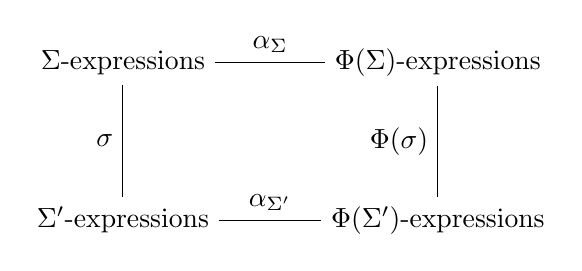
\begin{tikzpicture}[scale=2]
\node (S) at (0,1) {$\Sigma$-expressions};
\node (S') at (0,0) {$\Sigma'$-expressions};
\node (P) at (2,1) {$\Phi(\Sigma)$-expressions};
\node (P') at (2,0) {$\Phi(\Sigma')$-expressions};
\draw[-\arrowtip] (S) -- node[left]{$\ov{\sigma}$} (S');
\draw[-\arrowtip] (S) -- node[above]{$\alpha_\Sigma$} (P);
\draw[-\arrowtip] (P) -- node[left]{$\ov{\Phi(\sigma)}$} (P');
\draw[-\arrowtip] (S') -- node[above]{$\alpha_{\Sigma'}$} (P');
\end{tikzpicture}
\end{center}

In particular, recalling that $\Sen(\Sigma)$ contains those expressions that are sentences and that $\Sen(\sigma)$ is the restriction of $\ov{\sigma}$ to $\Sen(\Sigma)$:

\begin{center}
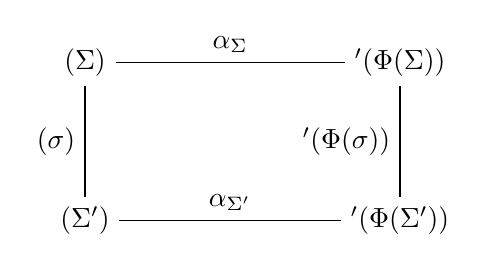
\begin{tikzpicture}[scale=2]
\node (S) at (0,1) {$\Sen(\Sigma)$};
\node (S') at (0,0) {$\Sen(\Sigma')$};
\node (P) at (2,1) {$\Sen'(\Phi(\Sigma))$};
\node (P') at (2,0) {$\Sen'(\Phi(\Sigma'))$};
\draw[-\arrowtip] (S) -- node[left]{$\Sen(\sigma)$} (S');
\draw[-\arrowtip] (S) -- node[above]{$\alpha_\Sigma$} (P);
\draw[-\arrowtip] (P) -- node[left]{$\Sen'(\Phi(\sigma))$} (P');
\draw[-\arrowtip] (S') -- node[above]{$\alpha_{\Sigma'}$} (P');
\end{tikzpicture}
\end{center}

It turns out, it these two are equal:

\begin{lemma}[Commutativity of $\Phi$ and $\alpha$]\label{lem:folhol:senmor}
For all $\sigma:\Sigma\arr\Sigma$ in $\Sig^{\FOLEQ}$, we have $\�{\alpha_\Sigma}{\ov{\Phi(\sigma)}}=\�{\ov{\sigma}}{\alpha_{\Sigma'}}$.
\end{lemma}
\medskip

A similar situation arises for the judgment and proof translation:

\begin{center}
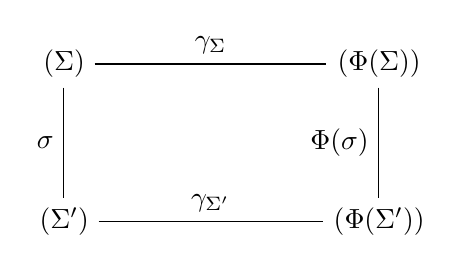
\begin{tikzpicture}[scale=2]
\node (S) at (0,1) {$\Pf^{\FOLEQ}(\Sigma)$};
\node (S') at (0,0) {$\Pf^{\FOLEQ}(\Sigma')$};
\node (P) at (2,1) {$\Pf^{\HOL}(\Phi(\Sigma))$};
\node (P') at (2,0) {$\Pf^{\HOL}(\Phi(\Sigma'))$};
\draw[-\arrowtip] (S) -- node[left]{$\ov{\sigma}$} (S');
\draw[-\arrowtip] (S) -- node[above]{$\gamma_\Sigma$} (P);
\draw[-\arrowtip] (P) -- node[left]{$\ov{\Phi(\sigma)}$} (P');
\draw[-\arrowtip] (S') -- node[above]{$\gamma_{\Sigma'}$} (P');
\end{tikzpicture}
\end{center}

Again it turns out, both are equal:

\begin{lemma}[Commutativity of $\Phi$ and $\gamma$]\label{def:folhol:ptmor}
For all $\sigma:\Sigma\arr\Sigma$ in $\Sig^{\FOLEQ}$, we have $\�{\gamma_\Sigma}{\ov{\Phi(\sigma)}}=\�{\ov{\sigma}}{\gamma_{\Sigma'}}$ both for judgments and for proofs.
\end{lemma}
\medskip

Finally, the corresponding situation -- but with reversed directions -- arises for the model translation:

\begin{center}
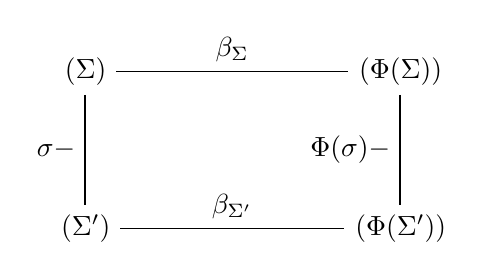
\begin{tikzpicture}[scale=2]
\node (S) at (0,1) {$\Mod^{\FOLEQ}(\Sigma)$};
\node (S') at (0,0) {$\Mod^{\FOLEQ}(\Sigma')$};
\node (P) at (2,1) {$\Mod^{\HOL}(\Phi(\Sigma))$};
\node (P') at (2,0) {$\Mod^{\HOL}(\Phi(\Sigma'))$};
\draw[\arrowtip-] (S) -- node[left]{$\reduce{\sigma}{-}$} (S');
\draw[\arrowtip-] (S) -- node[above]{$\beta_\Sigma$} (P);
\draw[\arrowtip-] (P) -- node[left]{$\reduce{\Phi(\sigma)}{-}$} (P');
\draw[\arrowtip-] (S') -- node[above]{$\beta_{\Sigma'}$} (P');
\end{tikzpicture}
\end{center}

Again it turns out, both are equal:

\begin{lemma}[Commutativity of $\Phi$ and $\beta$]\label{def:folhol:mtmor}
For all $\sigma:\Sigma\arr\Sigma$ in $\Sig^{\FOLEQ}$, we have $\�{\reduce{\Phi(\sigma)}{-}}{\beta_\Sigma}=\�{\beta_{\Sigma'}}{\reduce{\sigma}{-}}$ both for models \advanced{and model morphisms}.
\end{lemma}
\medskip

\section{Invariants}\label{sec:folhol:inv}

%However, that alone is not worth much yet: We could simply translation all judgments to a trivially true judgment $J$ one and all proofs to some proof of $J$. That would be a useless proof theory translation that nonetheless preserves provability. We need one additional requirement: The translation should also preserve proof theoretical truth. This is the content of the lemma:

As pointed out in Rem.~\ref{rem:folhol:pt}, the existence of $\gamma$ already guarantees that provability is preserved. Moreover, we observe:

\begin{lemma}[Commutativity of $\alpha$ and $\gamma$]
For all $\Sigma\in\Sig^{\FOLEQ}$ and all $F\in\Sen^{\FOLEQ}(\Sigma)$, we have
 \[\gamma_\Sigma(\val^{\FOLEQ}_\Sigma F)\; = \;\val^{\HOL}_{\Phi(\Sigma)}(\alpha_\Sigma(F)).\]
\end{lemma}
\begin{proof}
Directly from the definitions.
\end{proof}

Now we know that the validity of FOLEQ is translated to the validity judgment of HOL. Together with the proof-preservation of $\gamma$, we obtain the central theorem:

\begin{notation}
For $\Theta\sq\Sen(\Sen(\Sigma)$, we write $\alpha_\Sigma(\Theta)$ for $\{\alpha_\Sigma(F) : F\in\Theta\}$.
\end{notation}

\begin{theorem}[Preservation of Proof-Theoretical Consequence]
For all $\FOLEQ$-theories $(\Sigma,\Theta)$ and all $F\in\Sen(\Sigma)$, if $F$ is a proof theoretical theorem of $(\Sigma,\Theta)$, then $\alpha_\Sigma(F)$ is a proof theoretical theorem of $(\Phi(\Sigma),\alpha_\Sigma(\Theta))$.
\end{theorem}
\begin{proof}
Immediate.
\end{proof}


\begin{lemma}[Commutativity of $\alpha$ and $\beta$]\label{lem:folhol:mtinv}
For all $\Sigma\in\Sig^{\FOLEQ}$ and all $F\in\Sen^{\FOLEQ}(\Sigma)$, we have
 \[\moda[\FOLEQ]{\beta_\Sigma(I)}{\Sigma}{F}\tb\miff\tb\moda[\HOL]{I}{\Phi(\Sigma)}{\alpha_\Sigma(F)} \tb\mforall M\in\Mod^{\HOL}(\Phi(\Sigma)).\]
\end{lemma}

Now we know that the satisfaction relation of FOLEQ is translated to the satisfaction relation of HOL. This yields the central theorem:
\begin{theorem}[Preservation of Model-Theoretical Consequence]
For all $\FOLEQ$-theories $(\Sigma,\Theta)$ and all $F\in\Sen(\Sigma)$, if $F$ is a model theoretical theorem of $(\Sigma,\Theta)$, then $\alpha_\Sigma(F)$ is a model theoretical theorem of $(\Phi(\Sigma),\alpha_\Sigma(\Theta))$.
\end{theorem}
\begin{proof}
Assume $I\in\Mod^{\HOL}(\Phi(\Sigma))$ and $\moda[\HOL]{I}{\Phi(\Sigma)}{\alpha_\Sigma(A)}$ for all $A\in\Theta$ (*). We need to show $\moda[\HOL]{I}{\Phi(\Sigma)}{\alpha_\Sigma(F)}$. (*) and Lem.~\ref{lem:folhol:mtinv} yield $\moda[\FOLEQ]{\beta_\Sigma(I)}{\Sigma}{A}$ for all $A\in\Theta$. Therefore, using that $F$ is a model theoretical theorem of $(\Sigma,\Theta)$, we infer $\moda[\FOLEQ]{\beta_\Sigma(I)}{\Sigma}{F}$. Using Lem.~\ref{lem:folhol:mtinv} again, we obtain the needed property.
\end{proof}




\chapter{An Abstract Definition of a Logic Translation}\label{sec:trans:abs}
  Now we collect the definitions from Sect.~\ref{sec:folhol} and abstract from them. As before, we \advanced{distinguish} advanced material that can be ignored.

\section{Translations}

\begin{definition}[Syntax]
Given two logic syntaxes $(\Sig,\Sen)$ and $(\Sig',\Sen')$, we define a logic syntax translation as a pair $(\Phi,\alpha)$ such that
  \begin{itemize}
    \item $\Phi$ is a mapping
      \begin{itemize}
        \item $\Sig\arr\Sig'$
        \item \advanced{$\Sig(\Sigma_1,\Sigma_2)\arr\Sig'(\Phi(\Sigma_1),\Phi(\Sigma_2))$ for all $\Sigma,\Sigma'\in\Sig$}
      \end{itemize}
    \item $\alpha$ is a family of mappings $\alpha_\Sigma$ for $\Sigma\in\Sig$ such that
      \begin{itemize}
        \item $\alpha_\Sigma:\Sen(\Sigma)\arr\Sen'(\Phi(\Sigma))$
        \item \advanced{for all $\sigma:\Sigma\arr\Sigma'$ in $\Sig$, we have $\�{\alpha_\Sigma}{\Sen'(\Phi(\sigma))}=\�{\Sen(\sigma)}{\alpha_{\Sigma'}}$}
      \end{itemize}
  \end{itemize}
\end{definition}

\begin{definition}[Proof Theory]
Given two proof theoretical logics $(\Sig,\Sen,\Pf,\val)$ and $(\Sig',\Sen',\Pf',\val')$, and given a syntax translation $(\Phi,\alpha)$ between them, a proof theory translation $\gamma$
  \begin{itemize}
    \item is a family of mappings $\gamma_\Sigma$ for $\Sigma\in\Sig$ such that
      \begin{itemize}
        \item $\gamma_\Sigma$ is a mapping such that
          \begin{itemize}
            \item $\gamma_\Sigma:\Pf(\Sigma)\arr\Pf'(\Phi(\Sigma))$
            \item $\gamma_\Sigma:\Pf(\Sigma)((J_1,\ldots,J_m),J) \;\arr \; \Pf'(\Phi(\Sigma))((\gamma_\Sigma(J_1),\ldots,\gamma_\Sigma(J_m)),\gamma_\Sigma(J))$
          \end{itemize}
        \item \advanced{for all $\sigma:\Sigma\arr\Sigma'$ in $\Sig$, we have $\�{\gamma_\Sigma}{\Pf'(\Phi(\sigma))}=\�{\Pf(\sigma)}{\gamma_{\Sigma'}}$}
      \end{itemize}
    \item \advanced{such that for all $\Sigma\in\Sig$ and all $F\in\Sen(\Sigma)$
      \[\gamma_\Sigma(\val_\Sigma(F)) \;=\; \val'_{\Phi(\Sigma)}(\alpha_\Sigma(F))\]
      }
  \end{itemize}
\end{definition}


\begin{definition}[Model Theory]
Given two model theoretical logics $(\Sig,\Sen,\Mod,\md)$ and $(\Sig',\Sen',\Mod',\md')$, and given a syntax translation $(\Phi,\alpha)$ between them, a model theory translation $\gamma$
  \begin{itemize}
    \item is a family of mappings $\beta_\Sigma$ for $\Sigma\in\Sig$ such that
      \begin{itemize}
        \item $\beta_\Sigma$ is a mapping such that
          \begin{itemize}
            \item $\beta_\Sigma:\Mod'(\Phi(\Sigma))\arr\Mod(\Sigma)$
            \item \advanced{$\beta_\Sigma:\Mod'(\Phi(\Sigma))(M,N)\arr\Mod(\Sigma)(\beta_\Sigma(M),\beta_\Sigma(N))$}
          \end{itemize}
        \item \advanced{for all $\sigma:\Sigma\arr\Sigma'$ in $\Sig$, we have $\�{\Mod'(\Phi(\Sigma))}{\beta_\Sigma}=\�{\beta_\Sigma'}{\Mod(\sigma)}$}
      \end{itemize}
    \item \advanced{such that for all $\Sigma\in\Sig$ and all $F\in\Sen(\Sigma)$
       \[\moda{\beta_\Sigma(M)}{\Sigma}{F} \tb\miff\tb \moda[']{M}{\Phi(\Sigma)}{\alpha_\Sigma(F)} \tb \mfor M\in\Mod'(\Phi(\Sigma))\]
       }
  \end{itemize}
\end{definition}

\begin{remark}
Model theoretical logics are usually called \emph{institutions}. Model theory translations between institutions are usually called \emph{institution comorphisms}.
Institution morphisms also exists. Arguably, the names of morphisms and comorphisms should have better been swapped in this case.
\end{remark}


\begin{definition}[Logics]\label{def:trans:absmor}
Given two logics $L=(\Sig,\Sen,\Mod,\md,\Pf,\val)$ and $L'=(\Sig',\Sen',\Mod',\md',\Pf',\val')$, a \emph{logic translation} from $L$ to $L'$ consists of
\begin{itemize}
	\item a syntax translation $(\Phi,\alpha)$ from $(\Sig,\Sen)$ to $(\Sig',\Sen')$,
	\item a model theory translation $\beta$ extending $(\Phi,\alpha)$,
	\item a proof theory translation $\gamma$ extending $(\Phi,\alpha)$.
\end{itemize}
\end{definition}


\section{Preservation of Consequence}

In Sect.~\ref{sec:folhol:inv}, we proved two invariants about the logic translation from FOL to HOL. Both hold in general:

\begin{theorem}[Preservation of Proof-Theoretical Consequence]
Consider a proof theory translation $(\Phi,\alpha,\gamma):(\Sig,\Sen,\Pf,\val)\arr(\Sig',\Sen',\Pf',\val')$.
Moreover, consider a theory $(\Sigma,\Theta)$ and a sentence $F\in\Sen(\Sigma)$.
If $F$ is a proof theoretical theorem of $(\Sigma,\Theta)$, then $\alpha_\Sigma(F)$ is a proof theoretical theorem of $(\Phi(\Sigma),\alpha_\Sigma(\Theta))$.
\end{theorem}
\begin{proof}
\end{proof}

\begin{theorem}[Preservation of Model-Theoretical Consequence]
Consider a model theory translation $(\Phi,\alpha,\beta):(\Sig,\Sen,\Mod,\md)\arr(\Sig',\Sen',\Mod',\md')$.
Moreover, consider a theory $(\Sigma,\Theta)$ and a sentence $F\in\Sen(\Sigma)$.
If $F$ is a model theoretical theorem of $(\Sigma,\Theta)$, then $\alpha_\Sigma(F)$ is a model theoretical theorem of $(\Phi(\Sigma),\alpha_\Sigma(\Theta))$.
\end{theorem}
\begin{proof}
Assume $I\in\Mod'(\Phi(\Sigma))$ and $\moda[']{I}{\Phi(\Sigma)}{\alpha_\Sigma(A)}$ for all $A\in\Theta$. We need to show $\moda[']{I}{\Phi(\Sigma)}{\alpha_\Sigma(F)}$. By the properties of model theory translations, we obtain $\moda{\beta_\Sigma(I)}{\Sigma}{A}$ for all $A\in\Theta$. Therefore, using that $F$ is a model theoretical theorem of $(\Sigma,\Theta)$, we infer $\moda{\beta_\Sigma(I)}{\Sigma}{F}$. Using the properties of model theory translations again, we obtain the needed property.
\end{proof}

%theorems: borrowing of soundness, completeness; reflection of consequence for surjective translations
  
\chapter{Model Theories as Logic Translations}
  %%%%%%%%%%%%%%%%%%%%%%%%%%%%%%%%%%%%%%%%%%%%%%%%
\section{Models as Theory Morphisms}

In Sect.~\ref{sec:found:abs}, we have seen that foundations consist of a fixed theory in a fixed proof theoretical logic (along with some definition principles). Now consider a logic syntax $L=(\Sig,\Sen)$. We would like to define a model theory for it using a foundation consisting of $P$ and $\found$. The key observation is that the inductive definition of the interpretation function $\semm{-}{I}$ for a model $I$ behaves very much like the inductive expression translation function $\ov{\sigma}$ obtained from a theory morphism $\sigma$: Both are an inductive, compositional mapping in which every expression constructor of $L$ is mapped to a value constructor in mathematics. We want to make that precise and define models as theory morphisms. We can do that by using a special logic translation from $L$ to $P$:

\begin{definition}
Assume a logic syntax $L=(\Sig,\Sen)$ and a foundation $\found\in\Th^{P}$. A syntax translation $(\Phi,\alpha):L\arr P$ is called $\found$-founded if
\begin{itemize}
 \item $\Phi(\Sigma)$ is an extension of $\found$ for every $\Sigma\in\Sig$
 \item \advanced{$\Phi(\sigma)$ is the identity on $\found$ for every signature morphism $\sigma$}
\end{itemize}
\end{definition}

\begin{definition}\label{def:trans:modasmorph}
Assume a logic syntax $L=(\Sig,\Sen)$, a foundation $\found\in\Th^{P}$, and an $\found$-founded syntax translation $(\Phi,\alpha):L\arr P$. \\
We define $\Mod(\Sigma)$ as the collection of $P$-theory morphisms from $\Phi(\Sigma)$ to $\found$ that are the identity on $\found$. \\
Moreover, if $\sigma:\Phi(\Sigma)\arr\found$ is such a model and $F\in\Sen(\Sigma)$, we define
 \[\sigma\md_\Sigma F \tb\miff\tb \val^P_\found \ov{\sigma}(\alpha_\Sigma(F))\]
\end{definition}

\begin{remark}
More generally, for the interpretation function of $L$-$\Sigma$-expressions in the model $\sigma$, we obtain
 \[\semm{-}{\sigma}=\�{\alpha_\Sigma}{\ov{\sigma}}.\]
\end{remark}

\begin{remark}
More generally, we could use morphisms from $\Phi(\Sigma)$ to any conservative extension of $\found$ in Def.~\ref{def:trans:modasmorph}.
\end{remark}

\begin{theorem}\label{thm:trans:modasmorph}
Given a logic syntax $(\Sig,\Sen)$, a foundation $\found\in\Th^{P}$, and an $\found$-founded syntax translation $(\Phi,\alpha):L\arr P$. Then $(\Mod,\md)$ as defined in Def.~\ref{def:trans:modasmorph} is a model theory for $(\Sig,\Sen)$.
\end{theorem}

\begin{example}\label{ex:trans:modasmorph}
Consider $(\Sig^{\FOLEQ},\Sen^{\FOLEQ})$ and the foundation $HOLF\in\Th^{\HOL}$. We define a translation $(\Phi,\alpha)$ that is very similar to the one from Def.~\ref{def:folhol:syn} and~\ref{def:folhol:syn}. There are only two difference: (i) $\Phi(\Sigma)$ additionally contains all the declarations of $HOLF$; (ii) $\Phi(\Sigma)$ contains an additional base type $u$, which serves as the translation of the $\FOLEQ$-universe (instead of $\iota$).

For example, the $\FOLEQ$-signature of monoids is mapped to the $\HOL$ theory $M$ that extends $HOLF$ with
\begin{itemize}
  \item $u:\TYPE$,
  \item $\circ:u\arr u\arr u$
  \item $e:u$
\end{itemize}

Now a model of that signature is a $\HOL$-theory morphism from $M$ to $HOLF$ that is the identity on $HOLF$. Thus, every $HOLF$-symbol is mapped to itself, and we only have to map $u$, $\circ$, and $e$ is some way. That is exactly what a model is supposed to do.
\end{example}

\section{A More Abstract Formulation}

In order to formulate the notion of ``$\found$-founded translations'' more elegantly, we can use two constructions. Both work for arbitrary logics; therefore, we state them in full generality (which actually makes them more elegant).

\paragraph{The Logic of Theories}
For every logic $L$, we can construct another logic $\theolog{L}$ such that the signatures of $\theolog{L}$ are the theories of $L$.

\begin{definition}
Given a logic $L=(\Sig,\Sen,\Mod,\md,\Pf,\val)$, we define the logic $\theolog{L}=(\Th^L,\Sen',\Mod',\md',\Pf,\val')$ as follows:
\begin{itemize}
  \item $\Th^L$ consists of the theories and theory morphisms of $L$,
  \item $\Sen'$ is like $\Sen$ but ignores the axioms: $\Sen'((\Sigma;\Theta))=\Sen(\Sigma)$ and $\Sen'(\sigma)=\Sen(\sigma)$,
  \item $\Mod'(\Sigma;\Theta)$ is $\Mod(\Sigma;\Theta)$ from Def.~\ref{def:mod:models},
  \item $\md'_{(\Sigma,\Theta)}$ is the same as $\md_\Sigma$,
  \item $\Pf'(\Sigma;\Theta)$ has the same judgments as $\Pf(\Sigma)$, and all proofs may additionally use $\val_\Sigma F$ as assumptions for all $F\in\Theta$,
  \item $\val'_{(\Sigma,\Theta)}$ is the same $\val_\Sigma$
\end{itemize}

The corresponding definition applies to proof or model theoretical logics.
\end{definition}

\paragraph{The Logic of Extensions}
For every logic $L$ and a fixed signature $\Sigma$, we can construct another logic $\incllog{L}{\Sigma}$ that arises as as a sublogic of $L$: We only consider those signature that extend $\Sigma$.

\begin{definition}\label{def:logics:incllog}
Given a logic $L=(\Sig,\Sen,\Mod,\md,\Pf,\val)$ and a signature $\Sigma\in\Sig$, we define the logic $\incllog{L}{\Sigma}=(\Sig',\Sen',\Mod',\md',\Pf,\val')$ as follows:
\begin{itemize}
  \item $\Sig'$ consists of the signatures that extend $\Sigma$ and those signature morphisms between them that are the identity on $\Sigma$,
  \item $\Sen'$, $\Mod'$, $\md'$, $\Pf'$ and $\val'$ are the appropriate restrictions of their counterparts in $L$
\end{itemize}

The corresponding definition applies to proof or model theoretical logics.
\end{definition}

\begin{remark}
Technically, Def.~\ref{def:logics:incllog} only applies to logics in which \emph{signature inclusions} are a defined notion. This is not always the case, but almost always and almost always obviously so. For example, it is obvious what a signature inclusion in FOLEQ is.
\end{remark}

\paragraph{Founded Translations}
Now we can combine the two constructions:

\begin{lemma}
Assume a logic syntax $(\Sig,\Sen)$ and a foundation $\found\in\Th^{P}$. An $\found$-founded syntax translation $L\arr P$ is the same as a syntax translation $L\arr \incllog{\theolog{P}}{\found}$.
\end{lemma}

\begin{example}\label{ex:logics:incltheo}
Consider the logic $\incllog{\theolog{\FOLEQ}}{ZFC}$. Its ``signatures'' are the FOLEQ-theories that extend ZFC.
\end{example}


\part{A Proof-Theoretical Logical Framework}\label{part:lf}

\chapter{LF for Everybody}\label{sec:lffe}
 LF \cite{lf,logicalframeworks} is a logical framework, i.e., a formal language that we use to define other formal languages. It is a very advanced language, so advanced that we were only able to understand it in the 1980s. Therefore, it is very hard to learn and should only be attempted after gaining a solid basis of knowledge about logic. On the other hand, the intuitions underlying LF are strikingly simple and the precise definition of LF is actually quite short.

The major problem with learning LF is that LF goes together with a certain methodology of approaching logics. This methodology is so powerful and elegant that users of LF become very familiar with it, so much that they forget there is any other way to do it. Consequently, they often apply this methodology even when describing LF itself, thus scaring everybody off who has not embraced it yet. That makes it virtually impossible to learn LF on your own.

Therefore, we will go a different route here: We will ignore the foundations of LF altogether and focus on how we can use LF in practice. \emph{The goal is to show that LF is simple, natural, and practical rather than -- as many are inadvertently led to think -- difficult, weird, and esoteric.}

\section{The Context-Free Fragment}

\begin{quote}
 Lesson 1: LF is just a tool that we use to write down grammars. For convenience, we give the productions names.
\end{quote}

\paragraph{Grammars and Named Productions}
Consider the grammar of propositional logic over a fixed set $\Sigma$ of propositional variables:

\begin{center}
\begin{tabular}{lcl@{\tb}l}
$\FORM$ & $::=$ & $\true$ & \emph{truth} \\
     &  $|$  & $\false$ & \emph{falsity} \\
     &  $|$  & $\FORM \wedge \FORM$ & \emph{conjunction} \\
     &  $|$  & $\FORM \vee \FORM$ & \emph{disjunction} \\
     &  $|$  & $\FORM \impl \FORM$ & \emph{implication} \\
     &  $|$  & $\neg \FORM$ & \emph{negation} \\
     &  $|$  & $p$ where $p\in\Sigma$ & \emph{boolean variables}\\
\end{tabular}
\end{center}

Moreover, assume $p,q\in\Sigma$ and consider this example of a syntax tree for the formula $(\true\wedge p) \vee q$:

\begin{center}
\begin{tikzpicture}
\node (0) at (0,0) {$\FORM$};
\node (01) at (-1,-1) {$\FORM$};
\node (02) at (1,-1) {$\FORM$};
\node (011) at (-2,-2) {$\FORM$};
\node (012) at (0,-2) {$\FORM$};
\node (011') at (-2,-3) {$\true$};
\node (02') at (1,-2) {$q$};
\node (012') at (0,-3) {$p$};
\begin{scope}[gray]
\node (01t') at (-1,-2) {$\wedge$};
\node (0t') at (0,-1) {$\vee$};
\draw[dashed] (0) -- (0t');
\draw[dashed] (01) -- (01t');
\end{scope}
\draw[-\arrowtip] (0) -- (01);
\draw[-\arrowtip] (0) -- (02);
\draw[-\arrowtip] (01) -- (011);
\draw[-\arrowtip] (01) -- (012);
\draw[-\arrowtip] (02) -- (02');
\draw[-\arrowtip] (011) -- (011');
\draw[-\arrowtip] (012) -- (012');
\end{tikzpicture}
\end{center}

As usual, every node corresponds to a subformula of $(\true\wedge p) \vee q$ and is labelled with the non-terminal symbol with which the derivation of that subformula begins. In particular, the root corresponds to the whole formula and every leaf node to an atomic formula. Moreover, some nodes produce additional terminal symbols (given in gray).

The key property of a syntax tree is that every node is connected to its children via a production. With a tiny change, we are able to state that much more elegantly: We give the productions names.

Giving names to production is very natural, for example, we can use

\begin{center}
\begin{tabular}{lcl@{\tb}l}
$\FORM$ & $::=$ & $\rulename{truth} \rnsep \true$ & \\
     &  $|$  & $\rulename{falsity} \rnsep\false$ &  \\
     &  $|$  & $\rulename{conj} \rnsep \FORM \wedge \FORM$ &  \\
     &  $|$  & $\rulename{disj} \rnsep \FORM \vee \FORM$ &  \\
     &  $|$  & $\rulename{impl} \rnsep \FORM \impl \FORM$ &  \\
     &  $|$  & $\rulename{neg} \rnsep \neg \FORM$ & \\
     &  $|$  & $V_p \rnsep p$ where $p\in\Sigma$ \\
\end{tabular}
\end{center}

Note that naming the productions actually helps documenting and reading the grammar.

Now that the productions have names, we can use them to label the nodes in the syntax tree:

\begin{center}
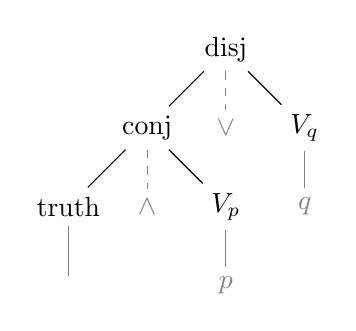
\begin{tikzpicture}
\node (0) at (0,0) {\rlname{disj}};
\node (01) at (-1,-1) {\rlname{conj}};
\node (02) at (1,-1) {$V_q$};
\node (011) at (-2,-2) {\rlname{truth}};
\node (012) at (0,-2) {$V_p$};
\begin{scope}[gray]
\node (01t') at (-1,-2) {$\wedge$};
\node (0t') at (0,-1) {$\vee$};
\node (011') at (-2,-3) {$\true$};
\node (02') at (1,-2) {$q$};
\node (012') at (0,-3) {$p$};
\draw[-\arrowtip] (02) -- (02');
\draw[-\arrowtip] (011) -- (011');
\draw[-\arrowtip] (012) -- (012');
\draw[dashed] (0) -- (0t');
\draw[dashed] (01) -- (01t');
\end{scope}
\draw[-\arrowtip] (0) -- (01);
\draw[-\arrowtip] (0) -- (02);
\draw[-\arrowtip] (01) -- (011);
\draw[-\arrowtip] (01) -- (012);
\end{tikzpicture}
\end{center}

Now we observe that the nodes for the terminal symbols are actually redundant. Indeed, if productions have names, we do not need terminal symbols (given in gray above) \emph{in a syntax tree}. Just like brackets, the sole purpose of $\wedge$ and $\vee$ is as a visual aid to display formulas nicely \emph{in a line}. And the terminal symbols like $\true$, $p$, and $q$ are redundant because they are determined by the name of the preceding production.

There is no commonly used convention how to write named productions in BNF. For example, we use an ad-hoc notation and write our grammar as follows:

\begin{center}
\begin{tabular}{lcl@{\tb}l}
$\FORM$ & $::=$ & $\rlname{truth} \rnsep $ & \\
     &  $|$  & $\rlname{falsity} \rnsep $ &  \\
     &  $|$  & $\rlname{conj} \rnsep \FORM, \FORM$ &  \\
     &  $|$  & $\rlname{disj} \rnsep \FORM, \FORM$ &  \\
     &  $|$  & $\rlname{impl} \rnsep \FORM, \FORM$ &  \\
     &  $|$  & $\rlname{neg} \rnsep \FORM$ & \\
     &  $|$  & $V_p \rnsep $ where $p\in\Sigma$ \\
\end{tabular}
\end{center}

This may look a bit unusual, but observe that it still contains the same information as our original grammar.

\paragraph{Grammars in LF}
Grammars with named productions can be written down in LF directly. The basic idea is that non-terminal symbols and (named) productions are introduced by one declaration each:
\begin{enumerate}
\item For a non-terminal symbol $A$, we write $\idecl{A}{\type}$.
\item For a production $A::=\rnsep A_1\;\ldots A_n$, we write $\idecl{P}{A_1\arr\ldots\arr A_n\arr A}$.
\end{enumerate}

Our grammar becomes
\begin{twelfsig}
\decl{\FORM}{\type} \\
\decl{\rlname{truth}}{\FORM}\\
\decl{\rlname{falsity}}{\FORM}\\
\decl{\rlname{conj}}{\FORM\arr\FORM\arr\FORM}\\
\decl{\rlname{disj}}{\FORM\arr\FORM\arr\FORM}\\
\decl{\rlname{impl}}{\FORM\arr\FORM\arr\FORM}\\
\decl{\rlname{neg}}{\FORM\arr\FORM}\\
\decl[$\mfor p\in\Sigma$]{V_p}{\FORM}\\
\end{twelfsig}
In LF text files, $\arr$ is written as $-\!\!>$.

One might argue that the notation with $\type$ and $\arr$ is somewhat arbitrary and even weird. Indeed, other notations can be more intuitive. Just for comparison, this is how the same grammar is written in SML:
\begin{lstlisting}[mathescape]
datatype $\FORM$ =
   $\rlname{truth}$
 | $\rlname{falsity}$
 | $\rlname{conj}$    of $\FORM$ * $\FORM$
 | $\rlname{disj}$    of $\FORM$ * $\FORM$
 | $\rlname{impl}$    of $\FORM$ * $\FORM$
 | $\rlname{neg}$    of $\FORM$ * $\FORM$
 | $\rlname{V_p}$                           for $p$ in $\Sigma$
\end{lstlisting}
Note how there is one \lstinline|datatype| for each non-terminal and one constructor for each production.

The specific notation of LF is in fact chosen very carefully and is very intuitive. But we will understand why only after learning a lot more about type theory.

\paragraph{Syntax Trees in LF}
In LF, we cannot only write down grammars but also syntax trees.
Our example tree from above is written in LF as
 \[(\rlname{conj}\;(\rlname{disj}\;\rlname{truth}\; V_p)\;V_q).\]
We only need brackets and whitespace to make sure that this linear representation can be uniquely translated back into a syntax tree.

This way of writing trees goes back to Lisp's S-expressions. It's also how SML does it. Some people might prefer the equivalent
\[\rlname{conj}(\rlname{disj}(\rlname{truth},V_p),V_q).\]

If we want to use XML, we can write a syntax tree like in OpenMath:
\begin{lstlisting}
<OMA>
  <OMS name="conj"/>
  <OMA><OMS name="disj"/><OMS name="truth"/><OMS name="V_p"/></OMA>
  <OMS name="V_q"/>
</OMA>
\end{lstlisting}

The bottom line is: We're now able to talk about syntax trees as objects! Instead of having to treat formulas as strings, we can treat them as syntax trees.

\section{The Context-Sensitive Fragment}\label{sec:lffe:cs}

\begin{quote}
 Lesson 2: It's useful to have productions that recurse into expressions with holes. LF supports that elegantly.
\end{quote}

Let's first understand what we mean by ``expressions with holes''.

\subsection{Expressions with Holes}\label{sec:lffe:holes}

\paragraph{Leaving Holes}
Consider our grammar for first-order logic:
\begin{center}
\begin{tabular}{lcl@{\tb}l}
$\FORM$ & $::=$ & $\true$ & \emph{truth} \\
        &  $|$  & $\false$ & \emph{falsity} \\
        &  $|$  & $\FORM \wedge \FORM$ & \emph{conjunction} \\
        &  $|$  & $\FORM \vee \FORM$ & \emph{disjunction} \\
        &  $|$  & $\FORM \arr \FORM$ & \emph{implication} \\
        &  $|$  & $\neg \FORM$ & \emph{negation} \\
        &  $|$  & $\forall \VAR\; \FORM$ & \emph{universal quantification} \\
        &  $|$  & $\exists \VAR\; \FORM$ & \emph{existential quantification} \\
        &  $|$  & $\TERM \doteq \TERM$ & \emph{equality} \\
        &  $|$  & $p(\overbrace{\TERM,\ldots,\TERM}^n)$ where $p\in\Sigma_p$ and $\arit(p)=n$& \emph{atomic formulas} \\
$\TERM$ & $::=$ & $f(\overbrace{\TERM,\ldots,\TERM}^n)$ where $f\in\Sigma_f$ and $\arit(f)=n$ & \emph{constants and function terms} \\
        &  $|$  & $\VAR$ & \emph{variables} \\
$\VAR$  & $::=$ & some countable set of names & \emph{variable names}
\end{tabular}
\end{center}

There is something fishy about this grammar, namely the non-terminal $\VAR$ with its vague production. This happens because -- contrary to propositional logic -- first-order logic is a language with binding, e.g., the $x$ is bound in $\forall x\;F$.
\medskip

Just like the named productions above, we can obtain a more elegant treatment of binding with a small conceptual leap: We introduce expressions with holes.

For example, let $F$ be the formula $f(x,y)\doteq g(y)$. $F$ has two variables -- $x$ and $y$ -- which we think of as placeholders for arbitrary terms. Let's make the placeholders explicit in the syntax tree:

\begin{center}
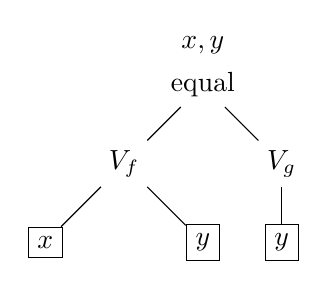
\begin{tikzpicture}
\node (H) at (0,.5) {$x,y$};
\node (0) at (0,0) {\rlname{equal}};
\node (01) at (-1,-1) {$V_f$};
\node (02) at (1,-1) {$V_g$};
\node[draw,rectangle] (011) at (-2,-2) {$x$};
\node[draw,rectangle] (012) at (0,-2) {$y$};
\node[draw,rectangle] (021) at (1,-2) {$y$};
\draw[-\arrowtip] (0) -- (01);
\draw[-\arrowtip] (0) -- (02);
\draw[-\arrowtip] (01) -- (011);
\draw[-\arrowtip] (01) -- (012);
\draw[-\arrowtip] (02) -- (021);
\end{tikzpicture}
\end{center}

The placeholder nodes are boxed to indicate that they do not represent productions but unknown subtrees that will be determined later.
To emphasize the holes in an expression, we will always list them above the root of the syntax tree.

\paragraph{Filling Holes}
Holes are placeholders for unknown expressions. Once known, we can plug in any expression for such a place holder. For example, in the expression $F$ above, we can plug the syntax tree for $f(c)$ into the hole $y$:

\begin{center}
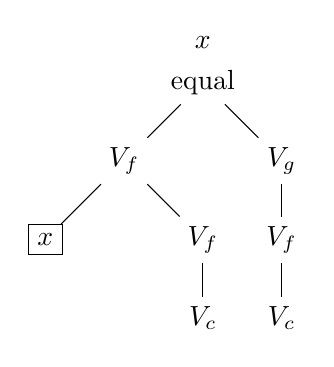
\begin{tikzpicture}
\node (H) at (0,.5) {$x$};
\node (0) at (0,0) {\rlname{equal}};
\node (01) at (-1,-1) {$V_f$};
\node (02) at (1,-1) {$V_g$};
\node[draw,rectangle] (011) at (-2,-2) {$x$};
\node (012) at (0,-2) {$V_f$};
\node (021) at (1,-2) {$V_f$};
\draw[-\arrowtip] (0) -- (01);
\draw[-\arrowtip] (0) -- (02);
\draw[-\arrowtip] (01) -- (011);
\draw[-\arrowtip] (01) -- (012);
\draw[-\arrowtip] (02) -- (021);
\node (0121) at (0,-3) {$V_c$};
\node (0211) at (1,-3) {$V_c$};
\draw[-\arrowtip] (012) -- (0121);
\draw[-\arrowtip] (021) -- (0211);
\end{tikzpicture}
\end{center}

Note that it is important that the holes are named: If a hole is used multiple times, we must plug in the same subtree everywhere. Also note that the resulting syntax tree only has one hole $x$.
\medskip

\paragraph{Expressions with Holes in General}
Of course, plugging in expressions for holes is exactly what we know already from first-order logic as the substitution of expressions for free variables. But note that we can use expressions with named holes \emph{for any grammar}. For example, let $G$ be the expression $a \impl (b \wedge a)$ of propositional logic with two holes $a$ and $b$; its syntax tree is

\begin{center}
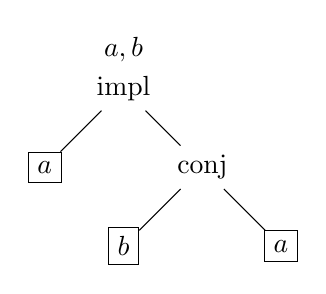
\begin{tikzpicture}
\node (H) at (0,.5) {$a,b$};
\node (0) at (0,0) {\rlname{impl}};
\node[draw,rectangle] (01) at (-1,-1) {$a$};
\node (02) at (1,-1) {\rlname{conj}};
\node[draw,rectangle] (021) at (0,-2) {$b$};
\node[draw,rectangle] (022) at (2,-2) {$a$};
\draw[-\arrowtip] (0) -- (01);
\draw[-\arrowtip] (0) -- (02);
\draw[-\arrowtip] (02) -- (021);
\draw[-\arrowtip] (02) -- (022);
\end{tikzpicture}
\end{center}

Note that we cannot generally plug in any subtree for any placeholder. For example, in $F$ above, we can only plug in terms for $x$ and $y$, i.e., a subtree whose root production is for the non-terminal $\TERM$. We call $\TERM$ the \emph{type} of the placeholders $x$ and $y$.

Let $H$ be the expression, $(f(x,y)\doteq g(y))\wedge a$; it has three holes, two of type $\TERM$ and one of type $\FORM$. Let's make the types explicit in our notation for syntax trees and write:

\begin{center}
\begin{tikzpicture}
\node (H) at (1,1.5) {$x:\TERM,y:\TERM,a:\FORM$};
\node (R) at (1,1) {\rlname{conj}};
\node[draw,rectangle] (R1) at (2,0) {$a$};
\node (0) at (0,0) {\rlname{equal}};
\node (01) at (-1,-1) {\rlname{V_f}};
\node (02) at (1,-1) {$V_g$};
\node[draw,rectangle] (011) at (-2,-2) {$x$};
\node[draw,rectangle] (012) at (0,-2) {$y$};
\node[draw,rectangle] (021) at (1,-2) {$y$};
\draw[-\arrowtip] (R) -- (0);
\draw[-\arrowtip] (R) -- (R1);
\draw[-\arrowtip] (0) -- (01);
\draw[-\arrowtip] (0) -- (02);
\draw[-\arrowtip] (01) -- (011);
\draw[-\arrowtip] (01) -- (012);
\draw[-\arrowtip] (02) -- (021);
\end{tikzpicture}
\end{center}

In this case, the types of the placeholders are redundant because the grammar forces us to plug in a term for $x$ and $y$ and a formula for $a$. It is still good to mark the types in the grammar: Firstly, it avoids confusion; secondly, the types are not always redundant.


\paragraph{Writing Expressions with Holes in LF}
LF lets us write expressions with holes explicitly. $G$ from above is written as
\[[a][b] (\rlname{impl}\;a\;(\rlname{\wedge}\;b\;a).\]
In LF, the holes of an expressions are always made explicit by prefixing the expressions with $[h]$ for every hole named $h$.

Again, we can argue about the notation. Some people prefer writing $G(a,b)$ or sometimes $G[a,b]$ if they want to emphasize that $G$ has two holes $a$ and $b$.

LF also lets us plug expressions into holes. If we want to plug in $\true$ for $a$ and $\false$ for $b$ in $G$, we write simply $G\;\true\;\false$. The result is the expression
\[G\;\true\;\false \;=\;\rlname{impl}\;\true\;(\rlname{\wedge}\;\false\;\true)\]
without holes.

Again, some people prefer the notation $G(\true,\false)$; that is incidental. The bottom line is: We can write expressions with holes easily and concisely in LF.
\medskip

LF also lets us make the types of placeholders explicit if we want to. For example, $H$ from above is written with explicit types as
\[[x:\TERM][y:\TERM][a:\FORM](\rlname{conj}\;(\rlname{equal}\;(V_f\;x\;y)\;y)\;a)\]

\subsection{Expressions with Holes as Operations}\label{sec:lffe:defs}

Every expression $E$ with a hole $x$ can be seen as an operation: The input is some other expressions $E'$; the output is the result of plugging $E'$ into the hole $E$. We can think of $E$ as a program, $E'$ as the input, and substitution as the machine that executes the program.

Since LF does substitution for us, we can directly use substitution to introduce some abbreviations. Consider the expression \[[a:\FORM][b:\FORM](\rlname{conj}\;(\rlname{impl}\;a\;b)\;(\rlname{impl}\;b\;a)),\]

In LF, we can introduce a name for any expression, with or without holes. If we want to call the expression above \rlname{equiv}, we write
\[\idecl{\rlname{equiv}}{\FORM\arr\FORM\arr\FORM \;=\;[a:\FORM][b:\FORM](\rlname{conj}\;(\rlname{impl}\;a\;b)\;(\rlname{impl}\;b\;a))}.\]

We can now write
 \[\rlname{equiv}\;\rlname{true}\;\rlname{false}\]
and substitution yields
  \[\rlname{equiv}\;\rlname{true}\;\rlname{false}\;=\;\rlname{conj}\;(\rlname{impl}\;\rlname{true}\;\rlname{false})\;(\rlname{impl}\;\rlname{false}\;\rlname{true})\]


\subsection{Productions using Expressions with Holes}

We've seen already that holes in expressions are nothing special. We usually call them \emph{free variables}, and they work in every grammar.

Using this intuition, we can now understand binding as an operation on expressions with holes.\footnote{This idea is called \emph{higher-order abstract syntax}. It is one of the most important ideas in the area of logical frameworks and a central principle of LF.} For example, we can understand the universal quantifier $\forall$ as an operator that takes a single argument: a formula with a hole of type $\TERM$.
\medskip

Again the BNF notation for grammars does not provide a notation for productions that use expressions with holes. Therefore, we have to introduce one ourselves again. Consider two non-terminals $A$ and $B$. Just like $B$ represents the collection of all expressions derived from $B$, we write $\{x:A\}B$ for the collection of all expressions derived from $B$ that have a hole named $x$ of type $A$.

For example, consider the production
 \[\FORM::=\rlname{conj}\rnsep\FORM\wedge\FORM.\]
We can read it as
\begin{center}
  ``The production \rlname{conj} takes two $\FORM$s and produces a $\FORM$.''
\end{center}
Similarly, we read the new production
 \[\FORM::=\rlname{univ}\rnsep\,\{x:\TERM\}\FORM\]
as
\begin{center}``The production \rlname{univ} takes a $\FORM$ with a hole $x$ for a $\TERM$ and produces a $\FORM$.''\end{center}
\medskip

With named productions and expressions with holes, our grammar for first-order logic becomes
\begin{center}
\begin{tabular}{lcl@{\tb}l}
$\FORM$ & $::=$
               & $\rlname{truth}\rnsep$ & \\
     &  $|$  & $\rlname{falsity}\rnsep$ &  \\
     &  $|$  & $\rlname{conj}\rnsep\FORM, \FORM$ &  \\
     &  $|$  & $\rlname{disj}\rnsep\FORM, \FORM$ &  \\
     &  $|$  & $\rlname{impl}\rnsep\FORM, \FORM$ &  \\
     &  $|$  & $\rlname{neg}\rnsep \FORM$ & \\
     &  $|$  & $\rlname{univ}\rnsep \{x:\TERM\} \FORM$ & \\
     &  $|$  & $\rlname{exist}\rnsep \{x:\TERM\} \FORM$ & \\
     &  $|$  & $\rlname{equal}\rnsep\TERM, \TERM$ &  \\
     &  $|$  & $V_p\rnsep\overbrace{\TERM,\ldots,\TERM}^n$ where $p\in\Sigma_p$ and $\arit(p)=n$& \\
$\TERM$ & $::=$ & $V_f\rnsep\overbrace{\TERM,\ldots,\TERM}^n$ where $f\in\Sigma_f$ and $\arit(f)=n$ & \\
        &  $|$  & $x$ & \\
\end{tabular}
\end{center}

For example, let $K$ be the formula $\forall x\;(p(x) \wedge \exists y\;q(u,y,v))$. Its syntax tree is

\begin{center}
\begin{tikzpicture}
\tikzstyle{bvar}=[dashed,rectangle,draw]
\tikzstyle{fvar}=[rectangle,draw]
\tikzstyle{level 3}=[sibling distance=3cm]
\tikzstyle{level 4}=[sibling distance=2cm]
\tikzstyle{edge from parent}+=[-\arrowtip]
\node at (0,.5) {$u:\TERM,v:\TERM$};
\path[level distance=1.3cm]
 node at (0,0) {\rlname{univ}}
  child {node {\rlname{conj}}
    child {node {$V_p$}
      child {node[bvar] {$x$}}
    }
	  child {node {\rlname{exist}}
	    child {node {$V_q$}
	      child {node[fvar] {$u$}}
        child {node[bvar] {$y$}}
        child {node[fvar] {$v$}}
        edge from parent node[right] {$y:\TERM$}
      }
    }
    edge from parent node[right] {$x:\TERM$}
  };
\end{tikzpicture}
\end{center}

Note how the nodes labelled with the productions $\rlname{univ}$ and $\rlname{exist}$ are followed by subtrees with holes. As before, the name of the hole is given above the respective subtree. Note that $x$ and $y$ are not holes of the overall tree; we say that they are \emph{bound}. To distinguish them from holes of the whole tree, we use dashed boxes for the bound holes.

%This grammar is not equivalent to the above grammar for first-order logic -- it is better. The above grammar permitted any formula as the argument to the universal quantification. Our new grammars permits exactly the terms with one hole.

\paragraph{Productions with Holes in LF}
We can write down our new grammar for first-order logic directly in LF:

\begin{twelfsig}
\decl{\FORM}{\type} \\
\decl{\TERM}{\type} \\
\decl{\rlname{truth}}{\FORM}\\
\decl{\rlname{falsity}}{\FORM}\\
\decl{\rlname{conj}}{\FORM\arr\FORM\arr\FORM}\\
\decl{\rlname{disj}}{\FORM\arr\FORM\arr\FORM}\\
\decl{\rlname{impl}}{\FORM\arr\FORM\arr\FORM}\\
\decl{\rlname{neg}}{\FORM\arr\FORM}\\
\decl{\rlname{equal}}{\TERM\arr\TERM\arr\FORM}\\
\decl{\rlname{univ}}{(\{x:\TERM\}\FORM)\arr\FORM}\\
\decl{\rlname{exist}}{(\{x:\TERM\}\FORM)\arr\FORM}\\
\decl[where $p\in\Sigma_p$ and $\arit(p)=n$]{V_p}{\overbrace{\TERM\arr\ldots\arr\TERM}^n\arr\;\FORM}  \\
\decl[where $f\in\Sigma_f$ and $\arit(f)=n$]{V_f}{\overbrace{\TERM\arr\ldots\arr\TERM}^n\arr\;\TERM} \\
\end{twelfsig}

%LF forces us to write $\{\_:\TERM\}\FORM$ instead of simply $\{\TERM\}\FORM$. There is a reason for that, and we will come back to it later.

The LF notation for syntax trees over these grammars is straightforward. For example, the formula $K$ is written in LF as 
\[[u:\TERM][v:\TERM]\;\rlname{univ}\;([x:\TERM]\;\rlname{conj}\;(p\;x)\;(\rlname{exist}\;([y:\TERM]\;V_q\;u\;y\;v)))\]
or -- if we omit the types of the placeholders -- as
\[[u][v]\;\rlname{univ}\;([x]\;\rlname{conj}\;(p\;x)\;(\rlname{exist}\;([y]\;V_q\;u\;y\;v)))\]

\section{Notation Declarations}

It is awkward to write syntax trees as
\[[u][v]\;\rlname{univ}\;([x]\;\rlname{conj}\;(p\;x)\;(\rlname{exist}\;([y]\;V_q\;u\;y\;v)))\]
because they are quite different from the nice notation
\[\forall x\;(p(x) \wedge \exists y\;q(u,y,v))\]
that we are used to. We can use a couple of syntactic sugars to tweak the LF notation into looking nicer.

\paragraph{Nice Identifiers}
We can give the productions any names we want. Most of the time, we can use the corresponding terminal symbol as the rule name. Moreover, we can use Unicode characters in identifiers. So we can change our grammar to

\begin{twelfsig}
\decl{\FORM}{\type} \\
\decl{\TERM}{\type} \\
\decl{\true}{\FORM}\\
\decl{\false}{\FORM}\\
\decl{\wedge}{\FORM\arr\FORM\arr\FORM}\\
\decl{\vee}{\FORM\arr\FORM\arr\FORM}\\
\decl{\impl}{\FORM\arr\FORM\arr\FORM}\\
\decl{\neg}{\FORM\arr\FORM}\\
\decldefnl{\equiv}{\FORM\arr\FORM\arr\FORM}{[a:\FORM][b:\FORM](\wedge\;(\impl\;a\;b)\;(\impl\;b\;a))} \\
\decl{\doteq}{\TERM\arr\TERM\arr\FORM}\\
\decl{\forall}{(\{x:\TERM\}\FORM)\arr\FORM}\\
\decl{\exists}{(\{x:\TERM\}\FORM)\arr\FORM}\\
\decl[where $p\in\Sigma_p$ and $\arit(p)=n$]{p}{\overbrace{\TERM\arr\ldots\arr\TERM}^n\arr\;\FORM}  \\
\decl[where $f\in\Sigma_f$ and $\arit(f)=n$]{f}{\overbrace{\TERM\arr\ldots\arr\TERM}^n\arr\;\TERM} \\
\end{twelfsig}
Note that we include the abbreviation for equivalence from Sect.~\ref{sec:lffe:defs}.

and now our example formula is written as
\[[u][v]\;\forall\;([x]\;\wedge\;(p\;x)\;\exists\;([y]\;q\;u\;y\;v)))\]

\paragraph{Notations}
We can also give notations to identifiers.
A notation consists of
\begin{itemize}
 \item fixity: prefix, infix (only for binary operators), or postfix
 \item if the fixity is infix, associativity: left, right, or none \\
   The associativity determines whether $P\;a\;Q\;a\;R$ is parsed as $(P\;a\;Q)\;a\;R$ (left), parsed as $P\;a\;(Q\;a\;R)$ (right), or forbidden (none).
   \footnote{Note that there is no such thing as an associative operator in LF.}
 \item precedence: a positive integer\\
  Higher precedences bind stronger, which permits omitting brackets.
\end{itemize}

We should make $\wedge$, $\vee$, $\impl$, $\equiv$, and $\doteq$ infix, and $\neg$ prefix.
$\wedge$ and $\vee$ should be left- or right-associative so that we can write $P\wedge Q\wedge R$. $\impl$ and $\equiv$ should have no associativity to avoid ambiguity.
$\neg$ should have a higher precedence than the other operators so that the brackets in $P\wedge (\neg Q)$ can be omitted. Finally, $\doteq$ should have a high precedence so that the brackets in $P\wedge (s\doteq t)$ can be omitted.

We can achieve that by adding the following notations to our grammar:

\begin{lstlisting}
%infix left 10 $\wedge$.
%infix left 10 $\vee$.
%infix none 10 $\impl$.
%infix none 10 $\equiv$.
%prefix 15 $\neg$.
%infix none 20 $\doteq$.
\end{lstlisting}

Then our example expression becomes:
\[[u][v]\;\forall\;([x]\;(p\;x)\wedge\exists\;([y]\;q\;u\;y\;v)))\]

Finally, LF uses the convention that the $[-]$ operator has the lowest possible precedence. Therefore, brackets around $([x]F)$ can often be omitted.
Our example expression finally becomes:
\[[u][v]\;\forall\;[x]\;(p\;x)\wedge\exists\;[y]\;(q\;u\;y\;v)\]

Note that this looks almost as nice as $\forall x\;(p(x) \wedge \exists y\;q(u,y,v))$. But the former is a syntax tree that we can work with directly whereas the latter is a string!


\section{The Fragment with Unary Dependent Types}

\begin{quote}
Lesson 3: It's often useful to have infinite families of non-terminals. LF supports that elegantly.
\end{quote}

Let's first understand why we would like to have infinitely many non-terminals.

\subsection{Families of Non-Terminals}

\paragraph{Proofs as Expressions}
So far we have seen how we can use LF to concisely write down context-sensitive grammars and expressions with holes. The main strength of LF is that we have a canonical linear notation for syntax trees of expressions.

In the area of logic, there is another kind of tree structure that is dominant: proofs. We have already seen how proofs can be represented as tree whose nodes are labelled with inference rules. Now we observe: This is basically the same principle as having syntax trees whose nodes are labelled with productions.

A production governs how we form new expressions from existing ones. Similarly, an inference rule governs how we form new proofs from existing ones. If we just think of them as syntax trees and productions, both of them become the same thing!

{\renewcommand{\der}{}
Compare a production, e.g., \rlname{impl}
\[\FORM::=\rlname{impl} \rnsep \FORM,\FORM\]
with an inference rule, e.g., modus ponens
\[\ibnc{\der F\impl G}{\der F}{\der G}{mp}\]
They look different, but that's just because we use very different notations. We see that if we write both of them as inference rules
\[
\ibnc{\FORM}{\FORM}{\FORM}{\rlname{impl}}
\tb\tb
\ibnc{\der F\impl G}{\der F}{\der G}{mp}
\]
or both of them as productions
\[
\FORM::=\rlname{impl} \rnsep \FORM,\FORM
\tb\tb
\der G \;::=\; mp \rnsep \der F\impl G, \;\der F
\]

\paragraph{Formulas as Non-Terminals}
However, there is one subtlety: In the case of inference rules, we do not have a finite set of non-terminal symbols. Indeed, the left side of the ``production'' for $mp$ is $\der G$ where $G$ is an arbitrary formula. Everything would work if we had a way of getting a fresh non-terminal symbol for every formula. But because we have infinitely many formulas, this is not possible right away.

Therefore, LF makes a third (after named productions and expressions with holes) key addition to our understanding of grammars: infinite families of non-terminal symbols. More concretely, if $A:\type$ is a non-terminal symbol, then we may add an $A$-indexed family $B$ of non-terminal symbols as $B:A\arr\type$.
}

For example, we introduce a $\FORM$-indexed family $\PROOF$ of non-terminal symbols as \[\PROOF:\FORM\arr\type.\] Then we have for every formula $F$ a non-terminal symbol $\PROOF\; F$. Expressions derived from $\PROOF\; F$ are the proofs of $F$.

Now we can in fact write our inference rule $mp$ like this
\[
\PROOF\; G \;::=\; mp \rnsep \PROOF\;(F\impl G), \;\PROOF\; F
\]

\subsection{Dependent Type Constructors in LF}

We have already seen the LF syntax for families of non-terminals above. For propositional logic, we declare our non-terminals as

\begin{twelfsig}
\decl{\FORM}{\type} \\
\decl{\PROOF}{\FORM\arr\type} \\
\end{twelfsig}

We can think of $\PROOF$ as an operator that takes one argument and returns a non-terminal symbol. Then ordinary non-terminals like $\FORM$ are the special case of non-terminals with $0$ arguments. In LF, we call the non-terminals \emph{types}. Non-terminals like $\PROOF\;F$ are called \emph{dependent types} because they depend on an expression.

The productions for $\FORM$ stay the same. And we want to write the production for $mp$ as 
\[\mathll{
\text{``$mp$ takes a proof of $F\impl G$ and a proof of $F$ and produces a proof of $G$.''}\nl[.5cm]
\ibnc{\der F\impl G}{\der F}{\der G}{mp}\nl[.5cm]
\idecl{mp}{\PROOF\;(F\impl G)\arr\PROOF\;F\arr\PROOF\;G}
}\]
\medskip

But there is still a small problem: In all three of the above formulations of the rule, $F$ and $G$ occur out of nowhere. We kind of know that they are intended to be arbitrary formulas, but we're not precise about it. Therefore, let's say
\begin{center}
``$mp$ takes a formula $F$, a formula $G$, a proof of $F\impl G$, and a proof of $F$\\ and produces a proof of $G$.''
\end{center}
Now we notice something special that was hidden by the notation before: $mp$ is a production that takes $4$ arguments, but \emph{the value of the first two arguments determines the type of the last two and of the return type}. This has become possible because of dependent types, and it is the most characteristic feature of dependent type theory.
\medskip

Therefore, we finally write $mp$ in LF as a production with two placeholders:
\[mp \;:\; \{F:\FORM\}\{G:\FORM\}\,\PROOF\;(F\impl G)\arr\PROOF\;F\arr\PROOF\;G\]
\medskip

Then our grammar for propositional logic looks like this:

\begin{twelfsig}
\decl{\FORM}{\type} \\
\decl{\PROOF}{\FORM\arr\type} \\[.5cm]
\decl{\rlname{truth}}{\FORM}\\
\decl{\rlname{falsity}}{\FORM}\\
\decl{\rlname{conj}}{\FORM\arr\FORM\arr\FORM}\\
\decl{\rlname{disj}}{\FORM\arr\FORM\arr\FORM}\\
\decl{\rlname{impl}}{\FORM\arr\FORM\arr\FORM}\\
\decl{\rlname{neg}}{\FORM\arr\FORM}\\
\decl[$\mfor p\in\Sigma$]{V_p}{\FORM}\\[.5cm]
\decl{mp}{\{F:\FORM\}\{G:\FORM\}\,\PROOF\;(F\impl G)\arr\PROOF\;F\arr\PROOF\;G} \\
\decl{\wedge E_l}{\{F:\FORM\}\{G:\FORM\}\,\PROOF\;(F\wedge G)\arr\PROOF\;F}\\
\decl{\wedge E_r}{\{F:\FORM\}\{G:\FORM\}\,\PROOF\;(F\wedge G)\arr\PROOF\;G}\\
\decl{\wedge I}{\{F:\FORM\}\{G:\FORM\}\,\PROOF\;F\arr\PROOF\;G\arr\PROOF\;(F\wedge G)} \\
\end{twelfsig}

Here we have already included the rules for conjunction:
\[\ianc{F\wedge G}{F}{\wedge E_l} \tb\tb \ianc{F\wedge G}{G}{\wedge E_r} \tb\tb \ibnc{F}{G}{F\wedge G}{\wedge I}\]

Of course, we're still missing all the other proof rules.
We could write them down already as well, but it's better to make the LF background a tiny bit more formal first using Sect.~\ref{sec:lffe:types}.
\medskip

Moreover, we can now declare axioms: An axiom asserting the formula $F$ is declared as a symbol that returns a proof of $F$. That makes sense because axioms are like additional proofs that exist a priori.

For example, consider the theory of semigroups is the first-order signature with a binary function symbol and an axiom for associativity. We obtain it by adding declarations to first-order logic, one for the function and one for the axiom:

\begin{twelfsig}
\tsig{Semigroup}\\
\decl[{\infix[$\circ$]{left}{30}}]{\circ}{\TERM\arr\TERM\arr\TERM}\\
\decl{\rlname{assoc}}{\PROOF\;\big(\forall [x] \forall[y]\forall[z] (x\circ y)\circ z \doteq x \circ (y\circ z)\big)} \\
\tsigend
\end{twelfsig}

Here we make use of an additional feature of Twelf: We can give a list of declarations a name using the keywork \lfkw{sig}.

Note that we give $\circ$ a higher precedence than $\doteq$ to save brackets.

\section{A Little More Background}\label{sec:lffe:types}

\subsection{Non-Terminals = Types}

The basic idea behind the formal syntax of LF is that we have two sorts of objects: expressions and types. \emph{Expressions} (sometimes also called \emph{terms}) represent syntax and proof trees. \emph{Types} classify the expressions; in particular, every non-terminal is a type. Every expression has exactly one type, and for an expression $E$ of type $T$, we write $E:T:\type$.

Thus, in order to understand the syntax of LF, we should understand what expressions and types there are. Let us review the different LF constructions that we have seen so far.

\begin{enumerate}
 \item Plain expressions representing syntax/proof trees. Their type is given by the non-terminal from which they are derived. E.g.,
   \[(\true\vee p)\wedge q\;:\;\FORM\;:\;\type.\]
 \item Expressions with holes
   \begin{itemize}
     \item Expressions with one hole. Their type is the form $\{x:A\}B$ where $A$ is the type of the hole $x$ and $B$ is the type of the whole expression. E.g.,
   \[[x:\TERM](x\;\doteq\;x)\;:\;\{x:\TERM\}\FORM\;:\;\type\]
  Note that a $[-]$-expression always has the corresponding $\{-\}$-type.
     \item Expressions with multiple holes are a special case: They are formed by chaining the above construction. E.g.,
   \[[x:\TERM][a:\FORM](x\;\doteq\;x)\wedge a\;:\;\{x:\TERM\}\{a:\FORM\}\FORM\;:\;\type\]
     \item Individual productions are expressions themselves. Their type is given in their declaration.
        E.g., $\neg:\FORM\arr\FORM$ is one of our productions, and we obtain
        \[\neg\;:\;\FORM\arr\FORM\;:\;\type\]
        When we write down LF formally, this becomes just a special case of an expression with a hole: Indeed, we \emph{define} $\FORM\arr\FORM$ as an abbreviation of $\{a:\FORM\}\FORM$ (for some arbitrary name $a$), and we employ the \emph{axiom}\footnote{This is called $\eta$-conversion.}
        \[\neg \; = \; [a:\FORM]\neg a\]
        That makes sense because $\neg$ and $[a:\FORM]\neg a$ behave in the same way according to $(\ast)$ below, namely
        \[\neg\;F \;=\; ([a:\FORM]\neg a)\;F.\]
   \end{itemize}
 \item Expressions formed by application
    \begin{itemize}
      \item Expressions formed by applying a production to another expression. Their type arises by removing one argument type. E.g., $\neg:\FORM\arr\FORM$ is a production that takes one argument of type $\FORM$, and if we apply it to another formula, we obtain
   \[\neg\;((\true\vee p)\wedge q)\;:\;\FORM\;:\;\type\]
      \item Expressions formed by applying a production to multiple expressions are a special case: They are formed by chaining the above construction, e.g.,
   \[\begin{array}{lclcl}
      mp & : & \{F:\FORM\}\{G:\FORM\}\,\PROOF\;(F\impl G)\arr \PROOF\;F\arr\PROOF\;G & : & \type\\
      mp\;\true & : & \{G:\FORM\}\,\PROOF\;(\true\impl G)\arr \PROOF\;\true\arr\PROOF\;G & : & \type\\
      mp\;\true\;p & : & \PROOF\;(\true\impl p)\arr \PROOF\;\true\arr\PROOF\;p & : & \type\\
    \end{array}\]
    and so on.
    \item Expressions formed by plugging an expression into a hole are a special case of application as well. Indeed, we have
    \[[a:\FORM]\neg a\;:\;\{a:\FORM\}\FORM\;:\;\type,\] and thus
    \[([a:\FORM]\neg a)\;F\;:\;\FORM\;:\;\type\]
    for any formula $F$. Note that we already know the result of plugging $F$ into the hole $a$, namely $\neg\;F$. Therefore, we employ the \emph{axiom}\footnote{This is called $\beta$-conversion.}
    \[([a:\FORM]\neg a)\;F \;=\;\neg\;F. \tb\tb(\ast)\]
  \end{itemize}
\end{enumerate}

\noindent
Note that we only need four basic constructions to form all the LF expressions:
\begin{enumerate}
 \item constants are atomic and must have been introduced by declarations; we distinguish the declarations
   \begin{enumerate}
     \item $a:\type$ and $b:A\arr\type$ for non-terminals and families of non-terminals, respectively,
     \item $c:A$ for some type $A$ productions,
   \end{enumerate}
 \item variables $x$ represent placeholders, they are atomic and can be used exactly in the scope of an abstraction $[x:A]\mathit{scope}$, for some type $A$
 \item abstractions represent terms with holes and are formed as $[x:A]t$,
 \item applications represent production application and are formed as $t\;t'$.
\end{enumerate}

\noindent
For the types, it is even easier: We only need two basic constructors:
\begin{enumerate}
 \item Atomic types arise from type declarations; we distinguish the 
   \begin{enumerate}
     \item base types $a$, which are declared as $a:\type$,
     \item dependent types $b\;t$, which are formed by applying a type family declared as $b:A\arr\type$ to a term $t$ of type $A$.
   \end{enumerate}
 \item The type $\{x:A\}B$ of expressions of type $B$ with a hole of type $A$ (equivalently: the type of operations that take a term of type $A$ and return a term of type $B$).
\end{enumerate}

\subsection{Types = Judgments}

Now that we know the types of LF types a bit better, let's get back to our types $\PROOF\;F$. There is something special about proofs: We often don't care about how many and what kinds of proofs of $F$, we have -- the most important thing is to know whether there is \emph{any} proof of $F$.\footnote{This attitude is called \emph{proof irrelevance}.} Consequently, we care about which of the following two is the case:
 \begin{enumerate}
   \item There is no proof of $F$, i.e., there is no term of type $\PROOF\;F$, i.e., the type $\PROOF\;F$ is empty.
   \item There is some proof of $F$, i.e., there is a term of type $\PROOF\;F$, i.e., the type $\PROOF\;F$ is non-empty.
 \end{enumerate}

It is very interesting to look at our types from that perspective.
\medskip

Let's start with the atomic types. We read the non-emptiness of the type $\PROOF\;F$ as ``$F$ has a proof.''. Thus, the type $\PROOF\;F$ expresses a judgment about $F$, namely the judgment
\begin{center}
$\PROOF\;F$ is non-empty\\ means \\ $F$ is provable.
\end{center}

Secondly, let us look at the special case $A\arr B$. (Recall: $A\arr B$ is an abbreviation for $\{x:A\}B$ for some unused name $x$.) We notice the following:
If the type $A\arr B$ is non-empty (i.e., there is a term $f:A\arr B$), then we have an operation that transforms terms of type $A$ (i.e., terms $t:A$) into terms of type $B$ (namely $f\;t:B$). Thus, we read 
\begin{center}
$A\arr B$ is non-empty\\ means \\ If $A$ is non-empty, then $B$ is non-empty. \\ or: $B$ is non-empty under the assumption that $A$ is non-empty.
\end{center}

For example, we read
\begin{center}
$\PROOF\;F\arr\PROOF\;G$ is non-empty\\ means \\ If $F$ is provable, then $G$ is provable. \\ or: $G$ is provable under the assumption that $F$ is provable.
\end{center}
More concretely, the type $\PROOF\;(F\wedge G)\arr\PROOF\;F$ (which is part of the rule $\wedge E_l$) expresses the judgment ``If $F\wedge G$ is provable, then $F$ is provable.'' We can also chain this construction, e.g., in the rule $\wedge I$, we write $\PROOF\;F\arr\PROOF\;G\arr\PROOF(F\wedge G)$ to say ``If $F$ and $G$ are provable, then $F\wedge G$ is provable''.

Thirdly, let us look at the case $\{x:A\}B$ where $x$ actually occurs in $B$. For example, consider the type $\{x:\FORM\}\PROOF\;x$.
If $\{x:A\}B$ is non-empty, we have a term $t:\{x:A\}B$, i.e., a term with a hole of type $A$ that yields a term of type $B\;t$ if we plug $t$ into the hole.
For example, if we have a term $\{x:\FORM\}\PROOF\;x$, then for any formula $F:\FORM$, plugging $F$ into the hole $x$ in $t$ yields a term of type $\PROOF\;F$.
Therefore, we read
\begin{center}
$\{x:A\}B$ is non-empty\\ means \\ For all $x:A$, the type $B\;x$ is non-empty. \\ or: $B\;x$ is non-empty for arbitrary $x$.
\end{center}
For example, we read
\begin{center}
$\{x:\FORM\}\PROOF\;x$ is non-empty\\ means \\ For all formulas $x$, $x$ is provable. \\ or: $x$ is provable for arbitrary $x$.
\end{center}
\medskip

Obviously, the judgment ``For all formulas $x$, $x$ is provable.'' is should not hold. The type $\{x:\FORM\}\PROOF\;x$ represents the judgment that our logic has a contradiction and should always be empty. We formalize this intuition in LF by adding the definition
\[\contra : \type = \{x:\FORM\}\PROOF\;x.\]


\section{Collecting the Pieces: A Logical Framework}

We are now ready to use LF to write down the remaining proof rules. The key trick is the intuition non-terminals, types, and judgments are all the same thing.

We will start with the rule for implication, negation, and universal quantification, which have a very nice property: They establish a back-and-forth mapping between the respective type $\PROOF\;F$ and some other type. More concretely, we have the following correspondence:

\begin{center}
\begin{tabular}{|l|l|l|}
\hline
proof type & represented as & intuition \\
\hline
$\PROOF\;(F\impl G)$ & $\PROOF\;F\arr\PROOF\;G$ & if $F$, then $G$ \\
$\PROOF\;(\neg F)$ & $\PROOF\;F\arr\contra$ & if $F$, then contradiction \\
$\PROOF\;(\forall[x:\TERM](F\;x))$ & $\{x:\TERM\}\PROOF\;(F\;x)$ & for arbitrary $x:\TERM$, $F\;x$\\
\hline
\end{tabular}
\end{center}

The introduction rules go from the representing type to the proof type. The elimination rules go the other way round.

\newcommand{\implicit}[1]{{\color{gray}#1}}

\paragraph{Implication}
Let's start with the implication introduction rule $\impl I$, which we can express in any one of the following ways:
\begin{center}
$\impl I$ takes \implicit{two formulas $F,G$}, a proof of $G$ with a hole for a proof of $F$ and produces a proof of $F\impl G$.\\[.5cm]
\implicit{For arbitrary $F,G$}, if $G$ is provable under the assumption that $F$ is provable, then $F\impl G$ is provable.\\[.5cm]
$\icnc{\implicit{F:\FORM}}{\implicit{G:\FORM}}{F\der G}{\der F\impl G}{\impl I}$\\[.5cm]
$\idecl{\impl I}{\implicit{\{F:\FORM\}\{G:\FORM\}}(\PROOF\; F\arr \PROOF\;G)\arr\PROOF\;(F\impl G)}$
\end{center}
Note how we are careful to introduce the arbitrary parameters $\implicit{F}$ and $\implicit{G}$. This is good practice. But it can get quite tedious to do that, and we will omit them later, see Sect.~\ref{sec:lffe:implicit}.

\noindent
We have already represented the implication elimination rule -- modus ponens:
\begin{center}
$\impl E$ takes \implicit{two formulas $F,G$}, a proof of $F\impl G$, and a proof of $F$ and produces a proof of $G$.\\[.5cm]
\implicit{For arbitrary $F,G$}, if $F\impl G$ and $F$ are provable, then $G$ is provable.\\[.5cm]
$\idnc{\implicit{F:\FORM}}{\implicit{G:\FORM}}{\der F\impl G}{\der F}{\der G}{\impl E}$\\[.5cm]
$\idecl{\impl E}{\implicit{\{F:\FORM\}\{G:\FORM\}}\PROOF\; (F\impl G)\arr \PROOF\;F\arr\PROOF\;G.}$
\end{center}

\paragraph{Negation}
The rule for negation introduction is similar to that of implication introduction. Intuitively, we already know it as proof by contradiction:
\begin{center}
$\neg I$ takes \implicit{a formula $F$} and a proof of contraction with a hole for a proof of $F$\\ and produces a proof of $\neg F$. \\[0.5cm]
\implicit{For arbitrary $F$}, if a contradiction is provable under the assumption that $F$ is provable,\\ then $\neg F$ is provable. \\[0.5cm]
$\ibnc{\implicit{F:\FORM}}{F\der \contra}{\der \neg F}{\neg I}$ \\[0.5cm]
$\idecl{\neg I}{\implicit{\{F:\FORM\}}(\PROOF\; F\arr \contra)\arr\PROOF\;(\neg F)}$
\end{center}

\noindent
The elimination rule for negation is straightforward -- we know it as contradiction:
\begin{center}
$\neg E$ takes \implicit{a formula $F$}, two proofs of $\neg F$ and $F$ and produces a contradiction.\\[.5cm]
\implicit{For arbitrary $F$}, if both $\neg F$ and $F$ are provable, then we have a contradiction.\\[.5cm]
$\icnc{\implicit{F:\FORM}}{\der \neg F}{\der F}{\der \contra}{\neg E}$\\[.5cm]
$\idecl{\neg E}{\implicit{\{F:\FORM\}}\PROOF\;(\neg F)\arr \PROOF\;F\arr\contra.}$
\end{center}

\paragraph{Universal Quantification}
Next we look at the rules for universally quantified formulas $\forall[x:\TERM](F\;x)$. Note that, here, $F$ is an arbitrary formula with a hole of type $\TERM$. The introduction rule $\forall I$ can be expressed as follows:
\begin{center}
$\forall I$ takes \implicit{a formula $F$ with a $\TERM$-hole}, and a proof of $F\;x$ with a $\TERM$-hole $x$ and produces a proof of $\forall[x:\TERM](F\;x)$.\\[.5cm]
\implicit{For an arbitrary formula $F$ with a $\TERM$-hole}, if $F\;x$ is provable for arbitrary $x:\TERM$, then $\forall[x:\TERM] (F\;x)$ is provable.\\[.5cm]
$\ibnc{\implicit{F:\{x:\TERM\}\FORM}}{x:\TERM\der F\;x}{\der \forall[x:\TERM] F\;x}{\impl I}$\\[.5cm]
$\idecl{\impl I}{\implicit{\{F:\{x:\TERM\}\FORM\}}\;\big(\{x:\TERM\}\PROOF\; (F\;x)\big)\arr \PROOF\;(\forall[x:\TERM](F\;x))}$
\end{center}

\noindent
The corresponding elimination rule is straightforward -- we know it as instantiation:
\begin{center}
$\forall E$ takes \implicit{a formula $F$ with a $\TERM$-hole}, a proof of $\forall[x:\TERM](F\;x)$, and a term $x$ and produces a proof of $F\;x$.\\[.5cm]
\implicit{For an arbitrary formula $F$ with a $\TERM$-hole}, if $\forall[x:\TERM](F\;x)$ is provable, then $F\;x$ is provable for any term $x$.\\[.5cm]
$\icnc{\implicit{F:\{x:\TERM\}\FORM}}{\der \forall[x:\TERM] F\;x}{x:\TERM}{\der F\;x}{\impl I}$\\[.5cm]
$\idecl{\impl I}{\implicit{\{F:\{x:\TERM\}\FORM\}}\;\PROOF\;(\forall[x:\TERM](F\;x))\arr \{x:\TERM\}\PROOF\; (F\;x)}$
\end{center}


\paragraph{Rules Remaining}
The six remaining rules are introduction and elimination for conjunction, disjunction, and existential quantification. They cannot be represented in the same nice way using a representing type. However, their representation is still very natural.

Introduction of conjunction and existential. These two behave similarly to pairing: To prove $F\wedge G$, we need a proof of $F$ \emph{and} a proof of $G$. To prove $\exists[x:\TERM](F\;x)$, we need a term $t$ \emph{and} a proof of $F\;t$. Consequently, the rules are

\begin{center}
$\idecl{\wedge I}{\implicit{\{F:\FORM\}\{G:\FORM\}}\PROOF\; F\arr \PROOF\;G\arr\PROOF\;(F\wedge G)}$\\[.5cm]
$\idecl{\exists I}{\implicit{\{F:\{x:\TERM\}\FORM\}} \{t:\TERM\}\PROOF\; (F\;t)\arr \PROOF\;(\exists[x:\TERM](F\;x))}$
\end{center}

Elimination of conjunction and introduction of disjunction. Here we need two pairs of rules -- one for the left and one for the right subformula. The resulting rules are dual:
\begin{center}
$\idecl{\wedge E_l}{\implicit{\{F:\FORM\}\{G:\FORM\}}\PROOF\; (F\wedge G)\arr \PROOF\;F}$ \\
$\idecl{\wedge E_r}{\implicit{\{F:\FORM\}\{G:\FORM\}}\PROOF\; (F\wedge G)\arr \PROOF\;G}$ \\[.5cm]
$\idecl{\vee I_l}{\implicit{\{F:\FORM\}\{G:\FORM\}}\PROOF\;F\arr\PROOF (F\vee G)}$ \\
$\idecl{\vee I_r}{\implicit{\{F:\FORM\}\{G:\FORM\}}\PROOF\;G\arr\PROOF (F\vee G)}$ \\
\end{center}

Elimination of disjunction and existential. These are the most difficult rules because there is an inherent indeterminism: If we have a proof of $F\vee G$, we know one of the two holds, but we do not know which one; similarly, if $\exists[x:\TERM](F\;x)$ holds, we know $F\;t$ holds for some $t$, but we do not know for which $t$. Therefore, we need to employ case distinction.

Let $C$ be the formula be the formula, we want to prove. If we want to use $F\vee G$ in the proof, we need to distinguish two cases:
\begin{center}
$\ifnc{\implicit{F:\FORM}}{\implicit{G:\FORM}}{\implicit{C:\FORM}}{\der F\vee G}{F\der C}{G\der C}{\der C}{\vee E}$\\[.5cm]
$\idecl{\vee E}{\implicit{\{F:\FORM\}\{G:\FORM\}\{C:\FORM\}}$\\ $\PROOF\; (F\vee G) \arr (\PROOF\;F\arr \PROOF\; C) \arr (\PROOF\;G\arr \PROOF\; C) \arr \PROOF\;C.}$
\end{center}

Similarly, if we want to use $\exists[x:\TERM](F\;x)$ in the proof of $C$, we need to distinguish one case for every possible $t$. We can merge all those cases into one proof with a hole for $t$:
\begin{center}
$\idnc{\implicit{F:\{x:\TERM\}\FORM}}{\implicit{C:\FORM}}{\der \exists[x:\TERM](F\;x)}{t:\TERM,\,F\;t\der C}{\der C}{\exists E}$\\[.5cm]
$\idecl{\exists E}{\implicit{\{F:\{x:\TERM\}\FORM\}\{C:\FORM\}}$ \\ $\PROOF\; \big(\exists[x:\TERM](F\;x)\big) \arr \big(\{t:\TERM\}\PROOF\;(F\;t)\arr \PROOF\; C\big) \arr\PROOF\;C.}$
\end{center}

\section{Proofs as Expressions}\label{sec:lffe:proofs}

We can now write natural deduction proofs directly as LF expressions. This is important because we do not have any other linear way to write formal proofs. The only alternative is the proof tree notation, which is elegant to read but awkward to write.

Consider the natural deduction proof of $(A\wedge B)\impl(B\wedge A)$. It looks like this
\newcommand{\seq}[2]{#1\vdash #2}

\[\rul{\seq{}{(A\wedge B)\impl(B\wedge A)}}{
    \rul{\seq{A\wedge B}{B\wedge A}}{
       \rul{\seq{A\wedge B}{B}}{
         \rul{\seq{A\wedge B}{A\wedge B}}{}{Axiom}
       }{\wedge E_r}
       \tb
       \rul{\seq{A\wedge B}{A}}{
         \rul{\seq{A\wedge B}{A\wedge B}}{}{Axiom}
       }{\wedge E_l}
    }{\wedge I}
  }{\impl I}
\]

Let's write this in a slightly more precise way by adding all the parameters of the proof rules, which we usually leave implicit:

\[\rul{\seq{}{(A\wedge B)\impl(B\wedge A)}}{
    \rul{\seq{A\wedge B}{B\wedge A}}{
       \rul{\seq{A\wedge B}{B}}{
         \rul{\seq{A\wedge B}{A\wedge B}}{}{Axiom\;\implicit{A\wedge B}}
       }{\wedge E_r\;\implicit{A\;B}}
       \tb
       \rul{\seq{A\wedge B}{A}}{
         \rul{\seq{A\wedge B}{A\wedge B}}{}{Axiom\;\implicit{A\wedge B}}
       }{\wedge E_l\;\implicit{A\;B}}
    }{\wedge I\;\implicit{B\;A}}
  }{\impl I\;\implicit{(A\wedge B)\;(B\wedge A)}}
\]

From such a proof, we can read off the corresponding LF term right away:

\[\impl I\;\implicit{(A\wedge B)\;(B\wedge A)}\;\big([p:\PROOF(A\wedge B)]\,
   \wedge I\;\implicit{B\;A}\;
      (\wedge E_l\;\implicit{A\;B}\;p)\;
      (\wedge E_r\;\implicit{A\;B}\;p)
\big)
\]

Note how the $\impl I$ rule, which introduces an assumption on the left of the $\vdash$, is represented as a term with a hole $p$. Moreover, whenever we refer to an assumption using the $Axiom$ rule, we simply give the name of hole. (In particular, we do not have to represent the $Axiom$ explicitly in LF -- we get automatically from the terms-with-holes formalism.)

We can add such a theorem to our formalism by using an abbreviation:

\begin{twelfsig}
\decldefnl{\wedge comm}{\{A:\FORM\}\{B:\FORM\}\;\PROOF\;\big((A\wedge B)\impl(B \wedge A)\big)}
{[A:\FORM][B:\FORM]\;\impl I\;\implicit{(A\wedge B)\;(B\wedge A)}\;\big([p:\PROOF(A\wedge B)]\,
   \wedge I\;\implicit{B\;A}\;
      (\wedge E_l\;\implicit{A\;B}\;p)\;
      (\wedge E_r\;\implicit{A\;B}\;p)
\big)
}
\end{twelfsig}

\section{Implicit Arguments}\label{sec:lffe:implicit}

We have already remarked above that we often do not mention some of the parameters in proof rules. For example, we prefer writing
\[\ianc{F\der G}{\der F\impl G}{\impl I}\]
to
\[\icnc{F:\FORM}{G:\FORM}{F\der G}{\der F\impl G}{\impl I}\]

Twelf supports that: We can write
\[\idecl{\impl I}{(\PROOF\; F\arr \PROOF\;G)\arr\PROOF\;(F\impl G)}\]
and Twelf will implicitly take it to mean
\[\idecl{\impl I}{\{F:\FORM\}\{G:\FORM\}(\PROOF\; F\arr \PROOF\;G)\arr\PROOF\;(F\impl G)}\]

More precisely: Whenever Twelf finds a free variable $F$ in a declaration, it will figure out the type $T$ of $F$ and place $\{F:T\}$ in front of the type.
$F$ is called an \emph{implicit argument}.

Twelf doing things automatically also means that sometimes errors go unnoticed. Therefore, Twelf uses the following convention: Variable names for implicit arguments must start with an upper case letter. Other free variables simply yield errors.
\medskip

Above, we have only said that proof rules do not have to declare parameters explicitly. The real power of Twelf is that when using a proof rule, we also do not have to provide the concrete values for these parameters -- Twelf figures them out based on the context.

For example, in the proof term given in Sect.~\ref{sec:lffe:proofs}, we can omit all the gray parts.

% \section{Morphisms}\label{sec:lffe:morph}


%\section{Conversions}
%beta and eta conversion to make the notation work

\chapter{Syntax of LF}
 We will now look at the logical framework LF (\cite{lf}) more formally. If you are already familiar with the Twelf implementation \cite{twelf} of LF, consider Fig.~\ref{fig:lftwelfsyntax} for the correspondence between the mathematical notation of LF and the ASCII notation of Twelf. LF is a type theory that arises from STT by adding the feature of \defemph{dependent types}. Dependent typing means that terms may occur in types. We will use that to represent proofs as terms and judgment as types: A constant declaration $\PROOF:\FORM \arr \TYPE$ returns a new type for every formula -- the type of proofs of that formula.

In dependent type theories, there are several type constructors. The most important one is the dependent function type. In a dependent function type, the value of the argument may occur in the return type. More generally, using functions with multiple arguments, the value of argument may occur in the later argument types and the return type. For example,
\[\P{F}{\FORM}\P{G}{\FORM}\PROOF\;F\arr\;\PROOF \;G\;\arr\PROOF\;(F\wedge G)\]
is the type of the conjunction introduction rule as a function taking two formulas and two proofs of them and returning a proof of the conjunction.

A good way to understand the syntax of LF is to compare it to the syntax of STT. The \defemph{judgments} of LF are almost the same as for STT. There are only two differences between STT and LF:
\begin{center}
	\begin{tabular}{|l|l|}
	  \hline
	  $\isdsig{\Sigma}$   & $\Sigma$ is a well-formed signature \\
	  $\ismorph{\Sigma}{\Sigma'}{\sigma}$  & $\sigma$ is a well-formed signature morphism from $\Sigma$ to $\Sigma'$ \\ $\isdcont{\Sigma}{\Gamma}$  & $\Gamma$ is a well-formed $\Sigma$-context \\
	  $\isdsubs{\Sigma}{\Gamma}{\Gamma'}{\gamma}$  & $\gamma$ is a well-formed substitution from $\Gamma$ to $\Gamma'$ over $\Sigma$ \\
		$\isdkind{\Sigma}{\Gamma}{K}$ & $K$ is a well-formed kind over $\Sigma$ and $\Gamma$ \\
		$\ofdkind{\Sigma}{\Gamma}{A}{K}$ & $A$ is a well-formed type family of (well-formed) kind $K$ over $\Sigma$ and $\Gamma$ \\
		$\ofdtype{\Sigma}{\Gamma}{t}{A}$ & $t$ is a well-formed term of (well-formed) type $A$ over $\Sigma$ and $\Gamma$ \\
		\hline
	\end{tabular}
\end{center}

The first difference is that LF adds a judgment for well-formed \defemph{kinds}. In type theories, the expressions are arranged in a hierarchy where the colon judgment $E:F$ is used if $F$ is one level above $E$ in the hierarchy. The first three levels have special names: level $0$ is the term level, level $1$ the type level, and level $2$ the kind level. We might call level $3$ the hyperkind level.

The kind level has the special kind $\TYPE$, which is the kind of all types. There may be more type-level expressions, which are then kinded by other kinds. Similarly, $\KIND$ is the hyperkind of all kinds.
If $E:F$ holds for a term $E$, then $F$ must be a type, i.e., $E:F:\TYPE$. Similarly, if $E$ is a type-level expression, then $F$ must be a kind and thus $E:F:\KIND$. We say terms are typed by types, and type-level expressions are kinded by kinds.

In STT, $\TYPE$ is the only kind, and all type-level expressions are types. Thus, kinds can be ignored. LF has more than one kind, and therefore, we need an extra judgment for well-formed kinds. The additional type level expressions are called type families. Thus, LF has typed terms and kinded type families.

The second difference is the judgment for well-formed type families. It now depends on a context $\Gamma$ because terms (and thus variables) can occur in types.

The context-free \defemph{grammar} also looks very similar:
\begin{center}
	\begin{tabular}{l@{\tb::=\tb}l}
		$\Sigma$ & $\cdot \| \Sigma,\;c:A \| \Sigma,\;a:K$ \\
		$\sigma$ & $\cdot \| \sigma,\;c:=t \| \sigma,\;a:=A$ \\
		$\Gamma$ & $\cdot \| \Gamma,\;x:A$ \\
		$\gamma$ & $\cdot \| \gamma,\;x/t$ \\
		$K$      & $\TYPE \| A\arr K$ \\
		$A$    & $a       \| A\;t \| \P{x}{A}A$ \\
		$t$      & $c     \| x \| t\;t \| \lam{x}{A}t$ \\
	\end{tabular}
\end{center}

The first difference between the grammars is that signatures may contain type family declarations $a:K$, not just base type declaration $a:\TYPE$. This is a natural consequence of using kinds.

The second difference is the extra non-terminal $K$ for kinds. A kind is either the special kind $\TYPE$ or of the form $A\arr K$. It is easy to see that all kinds are of the form $A_1\arr\ldots\arr A_n\arr\TYPE$. The intuition of such a kind is that a type family constant $a:A_1\arr\ldots\arr A_n\arr\TYPE$ takes $n$ arguments of types $A_1,\ldots,A_n$ and returns a type. This also means that other imaginable kinds are excluded: For example, there is no kind $\TYPE\arr\TYPE$ as we would need for a type operator like $list$.

The third difference are the productions for type families. The $\arr$ is gone, instead we have a $\Pi$, and we add an application $A\;t$ of type families to terms. The application is easy to understand: If we have $A:B\arr\TYPE$ and $t:B$, then we need a way to apply $A$ to $t$ in order to get a type -- that application is $A\;t$. The $\Pi$ is the dependent function type constructor. Intuitively, $\P{x}{A}B$ is the type of functions that take an argument $x$ of type $A$ and return a value of type $B(x)$ that depends on the value of the argument. Types of functions with multiple arguments are formed by chaining $\Pi$ just like chaining $\arr$ in STT: $\P{x_1}{A_1}\ldots\P{x_n}{A_n}B$ is the type of functions taking $n$ arguments $x_i$ of type $A_i$ and returning a value of type $B$ where every argument $x_i$ may occur in all later argument types $A_{i+1},\ldots,A_n$ and the return type $B$. The $\arr$ of STT is recovered as a special case: If in $\P{x}{A}B$, $x$ does not occur in $B$, we abbreviate it as $A\arr B$.

Intuitively, we have:
\begin{itemize}
	\item Signatures are lists of typed constants ($c:A$) and kinded type families ($a:K$).
	\item Signature morphisms are lists of terms and type families to be substituted for the symbols of a signature.
	\item Contexts are lists of typed variables ($x:A$). (As in STT, there are no kinded variables.)
	\item Substitutions are lists of terms to be substituted for the variables ($x/t$).
	\item Kinds are of the form $A_1\arr\ldots\arr A_n\arr\TYPE$ (just writing $\TYPE$ if $n=0$).
	\item Types are base types ($a$), application of type families to terms ($A\;t$) or dependent function types ($\P{x}{A}B$).
	\item Terms are constants ($c$), variables ($x$), dependent function applications ($f\;t$), or dependent $\lambda$-abstractions ($\lam{x}{A}t$).
\end{itemize}


\begin{example}
The following signature represents some operations on matrices.
\begin{itemize}
	\item A type for natural numbers with $1$ and successor: $N:\TYPE,\;1:N,\;s:N\arr N$. Here $s:N\arr N$ abbreviates $s:\P{x}{N}N$.
	\item A type family for matrices: $Mat:N\arr N\arr\TYPE$. $Mat$ takes two natural numbers, say $m$ and $n$, and returns a new type -- the type of $(m,n)$-matrices (over same ring which we omit).
	\item A constant for addition of matrices:
	 \[+:\P{x}{N}\P{y}{N}Mat\;x\;y\arr Mat\;x\;y\arr Mat\;x\;y.\]
	 $+$ first takes two natural numbers $x$ and $y$ and then two matrices with the dimensions $(x,y)$, i.e., two elements of type $Mat\;x\;y$, and returns another such matrix.
	\item A constant for multiplication of matrices: 
	\[\cdot:\P{x}{N}\P{y}{N}\P{z}{N}Mat\;x\;y\arr Mat\;y\;z\arr Mat\;x\;z.\]
	 $\cdot$ first takes three natural numbers $x$, $y$, and $z$ and then two matrices with the dimensions $(x,y)$ and $(y,z)$ and returns a matrix of dimension $(x,z)$.
\end{itemize}
Here is the declaration of $+$ again without the $\arr$ abbreviation and with some more brackets:
\[+\;\;:\;\;\P{x}{N}\big(\P{y}{N}\big(\P{m}{(Mat\;x)\;y}\big(\P{n}{(Mat\;x)\;y}\big((Mat\;x)\;y\big)\big)\big)\big)\]
\end{example}

The inference system for these judgments is more complicated than the one for STT because all judgments (except for signature morphisms) have to be defined by mutual recursion. This is because terms occur in types, types occur in kinds, and types and kinds occur in contexts and signatures -- on the other hand well-formed terms, type families, and kinds are defined relative to a signature and a context. It is even worse: Even substitution application must be part of that big mutual recursion because it is needed already in some of the rules.

This big mutual recursion can be hard to grasp for a beginner. Apart from that, it is quite straightforward. The rules are given in Fig.~\ref{fig:lf:signatures} and~\ref{fig:lf:terms}. Some expressions are underlined as a visual aid to make the bracketing structure apparent.

\begin{fignd}{lf:signatures}{Well-formed Signatures, Morphisms, Contexts, and Substitutions}
\ianc{}
     {\issig{\cdot}}
     {sigempty}
\tb\tb
\icnc{\issig{\Sigma}}
     {c \mnot\minn \Sigma}
     {\ofdkind{\Sigma}{\cdot}{A}{\TYPE}}
     {\issig{\Sigma,\;c:A}}
     {sigcon}
\tb\tb
\icnc{\issig{\Sigma}}
     {a \mnot\minn \Sigma}
     {\isdkind{\Sigma}{\cdot}{K}}
     {\issig{\Sigma,\;a:K}}
     {sigtype}
\\
\ianc{\issig{\Sigma'}}
     {\ismorph{\cdot}{\Sigma'}{\cdot}}
     {morphempty}
\tb\tb
\ibnc{\ismorph{\Sigma}{\Sigma'}{\sigma}}
     {\ofdtype{\Sigma'}{\cdot}{t}{\ov{\sigma}(A)}}
     {\ismorph{\underline{\Sigma,\;c:A}}{\Sigma'}{\underline{\sigma,\;c:=t}}}
     {morphcon}
\tb\tb
\ibnc{\ismorph{\Sigma}{\Sigma'}{\sigma}}
     {\ofdkind{\Sigma}{\cdot}{A}{\ov{\sigma}(K)}}
     {\ismorph{\underline{\Sigma,\;a:K}}{\Sigma'}{\underline{\sigma,\;a:=A}}}
     {morphtype}
\\
\ianc{\issig{\Sigma}}
     {\isdcont{\Sigma}{\cdot}}
     {conempty}
\tb\tb
\ibnc{\isdcont{\Sigma}{\Gamma}}
     {\ofdkind{\Sigma}{\Gamma}{A}{\TYPE}}
     {\isdcont{\Sigma}{\Gamma,\;x:A}}
     {convar}
\\
\ianc{\iscont{\Sigma}{\Gamma'}}
     {\issubs{\Sigma}{\cdot}{\Gamma'}{\cdot}}
     {subsempty}
\tb\tb
\ibnc{\issubs{\Sigma}{\Gamma}{\Gamma'}{\gamma}}
     {\ofdtype{\Sigma}{\Gamma'}{t}{\ov{\gamma}(A)}}
     {\issubs{\Sigma}{\underline{\Gamma,\;x:A}}{\Gamma'}{\underline{\gamma,\;x/t}}}
     {subsvar}
\end{fignd}

Note that the types and kinds of the constants in signatures must be closed, i.e., be well-formed in the empty context. In a context, however, the type of a variable may refer to the preceding variables. Therefore, when defining substitutions, we have to already apply the substitution to the types of the domain context in rule $subsvar$.


\begin{fignd}{lf:terms}{Well-formed Kinds, Type Families, and Kinds}
\ianc{\isdcont{\Sigma}{\Gamma}}
     {\isdkind{\Sigma}{\Gamma}{\TYPE}}
     {kdbase}
\tb\tb
\ibnc{\ofdkind{\Sigma}{\Gamma}{A}{\TYPE}}
     {\isdkind{\Sigma}{\Gamma}{K}}
     {\isdkind{\Sigma}{\Gamma}{A\arr K}}
     {kdfun}
\\
\ibnc{\isdcont{\Sigma}{\Gamma}}
     {a:K\minn \Sigma}
     {\ofdkind{\Sigma}{\Gamma}{a}{K}}
     {tpbase}
\tb\tb
\ibnc{\ofdkind{\Sigma}{\Gamma}{C}{A\arr K}}
     {\ofdtype{\Sigma}{\Gamma}{t}{A}}
     {\ofdkind{\Sigma}{\Gamma}{C\;t}{K}}
     {tpapp}
\\
\ibnc{\ofdkind{\Sigma}{\Gamma}{A}{\TYPE}}
     {\ofdkind{\Sigma}{\Gamma,x:A}{B}{\TYPE}}
     {\ofdkind{\Sigma}{\Gamma}{\P{x}{A}B}{\TYPE}}
     {tpfun}
\\
\ibnc{c:A \minn \Sigma}
     {\isdcont{\Sigma}{\Gamma}}
     {\ofdtype{\Sigma}{\Gamma}{c}{A}}
     {termcon}
\tb\tb
\ibnc{x:A\minn \Gamma \mtext{(rightmost} x \mtext{if\;multiple)}}
     {\isdcont{\Sigma}{\Gamma}}
     {\ofdtype{\Sigma}{\Gamma}{x}{A}}
     {termvar}
\\
\ibnc{\ofdtype{\Sigma}{\Gamma}{f}{\P{x}{A}B}}
     {\ofdtype{\Sigma}{\Gamma}{t}{A}}
     {\ofdtype{\Sigma}{\Gamma}{f\;t}{B[\sub{x}{t}]}}
     {termapp}
\tb\tb
\ianc{\ofdtype{\Sigma}{\Gamma,\;x:A}{t}{B}}
     {\ofdtype{\Sigma}{\Gamma}{\lam{x}{A}t}{\P{x}{A}B}}
     {termlam}
\end{fignd}

The rules for terms almost look like the ones from STT, but note that variables may now occur in the types. Therefore, substitution application is needed in rule $termapp$.

\begin{definition}[Substitution Application]\label{def:lf:subsapp}
For a substitution $\gamma=x_1/t_1,\ldots,x_n/t_n$, and a term, type family, or kind using only the variables $x_1,\ldots,x_n$, we define $\ov{\gamma}(-)$ as follows:
\begin{itemize}
     \item $\ov{\gamma}(\TYPE)=\TYPE$,
     \item $\ov{\gamma}(A \arr K)=\ov{\gamma}(A) \arr{\gamma}(K)$,
     \item $\ov{\gamma}(a)=a$,
     \item $\ov{\gamma}(A\;t)=\ov{\gamma}(A)\;\ov{\gamma}(t)$,
     \item $\ov{\gamma}(\P{x}{A}t)=\P{x}{\ov{\gamma}(A)}\ov{\gamma^x}(t)$,
     \item $\ov{\gamma}(c)=c$,
     \item $\ov{\gamma}(x_i)=t_i$,
     \item $\ov{\gamma}(f\;t)=\ov{\gamma}(f)\;\ov{\gamma}(t)$,
     \item $\ov{\gamma}(\lam{x}{A}t)=\lam{x}{\ov{\gamma}(A)}\ov{\gamma^x}(t)$,
\end{itemize}
where $\gamma^x$ abbreviates $\gamma,x/x$.
\end{definition}
We also write $t[x/s]$ for the result of substituting $x$ with $s$ and all other variables with themselves.

\begin{lemma}[Substitution Application]\label{lem:lf:subsapp}
Assume $\issubs{\Sigma}{\Gamma}{\Gamma'}{\gamma}$.
Then
\[\ofdtype{\Sigma}{\Gamma}{t}{A} \tb\mimplies\tb \ofdtype{\Sigma}{\Gamma'}{\ov{\gamma}(t)}{\ov{\gamma}(A)}\]
\[\ofdkind{\Sigma}{\Gamma}{A}{K} \tb\mimplies\tb \ofdkind{\Sigma}{\Gamma'}{\ov{\gamma}(A)}{\ov{\gamma}(K)}\]
\[\isdkind{\Sigma}{\Gamma}{K} \tb\mimplies\tb \isdkind{\Sigma}{\Gamma'}{\ov{\gamma}(K)}\]
\end{lemma}
\begin{proof}
One big induction.
\end{proof}

Similarly, we define signature morphism application.

\begin{definition}[Morphism Application]\label{def:lf:morapp}
Assume a signature morphism $\ismorph{\Sigma}{\Sigma'}{\sigma}$. Then, for a $\Sigma$ term, type family, or kind we define $\ov{\sigma}(-)$ as follows:
\begin{itemize}
     \item $\ov{\sigma}(\TYPE)=\TYPE$,
     \item $\ov{\sigma}(A \arr K)=\ov{\sigma}(A) \arr{\sigma}(K)$,
     \item $\ov{\sigma}(a)=A$ where $a:=A$ in $\sigma$,
     \item $\ov{\sigma}(A\;t)=\ov{\sigma}(A)\;\ov{\sigma}(t)$,
     \item $\ov{\sigma}(\P{x}{A}B)=\P{x}{\ov{\sigma}(A)}\ov{\sigma}(B)$,
     \item $\ov{\sigma}(c)=t$ where $c:=t$ in $\sigma$,
     \item $\ov{\sigma}(x)=x$,
     \item $\ov{\sigma}(f\;t)=\ov{\sigma}(f)\;\ov{\sigma}(t)$,
     \item $\ov{\sigma}(\lam{x}{A}t)=\lam{x}{\ov{\sigma}(A)}\ov{\sigma}(t)$.
\end{itemize}
\end{definition}

Like for STT, we only care about applying morphisms to closed expressions and map (bound) variables to themselves.

\begin{lemma}[Morphism Application]\label{lem:lf:morapp}
Assume $\ismorph{\Sigma}{\Sigma'}{\sigma}$. Then
\[\ofdtype{\Sigma}{\cdot}{t}{A} \tb\mimplies\tb \ofdtype{\Sigma'}{\cdot}{\ov{\sigma}(t)}{\ov{\sigma}(A)}\]
\[\ofdkind{\Sigma}{\cdot}{A}{K} \tb\mimplies\tb \ofdkind{\Sigma}{\cdot}{\ov{\sigma}(A)}{\ov{\sigma}(K)}\]
\[\isdkind{\Sigma}{\cdot}{K} \tb\mimplies\tb \isdkind{\Sigma}{\cdot}{\ov{\sigma}(K)}\]
\end{lemma}
\begin{proof}
Another big induction.

We actually use a more general theorem as the induction hypothesis:
\[\ofdtype{\Sigma}{\Gamma}{t}{A} \tb\mimplies\tb
\ofdtype{\Sigma'}{\ov{\sigma}(\Gamma)}{\ov{\sigma}(t)}{\ov{\sigma}(A)}\]
\[\ofdkind{\Sigma}{\Gamma}{A}{K} \tb\mimplies\tb \ofdkind{\Sigma}{\ov{\sigma}(\Gamma)}{\ov{\sigma}(A)}{\ov{\sigma}(K)}\]
\[\isdkind{\Sigma}{\Gamma}{K} \tb\mimplies\tb
\isdkind{\Sigma}{\ov{\sigma}(\Gamma)}{\ov{\sigma}(K)}\]
\[\iscont{\Sigma}{\Gamma} \tb\mimplies\tb
\iscont{\Sigma}{\ov{\sigma}(\Gamma)}\]

Here we define $\ov{\sigma}(\Gamma)$ (the homomorphic translation of a context along a signature morphism) by
\[\ov{\sigma}(\cdot) = \cdot\]
\[\ov{\sigma}(\Gamma,\,x:A) = \ov{\sigma}(\Gamma),\,x:\ov{\sigma}(A)\]
\end{proof}


\chapter{Semantics of LF}
 LF does not have formulas or a consequence relation between them. Therefore, LF is not a logic. Nevertheless, LF is a type theory, and every type theory has a semantics. As for logics, there is a proof- and a model-theoretical approach to define the semantics.

\section{Model-Theoretic Semantics}

The model theory of LF can be defined very similarly to the model theory of STT.

Just like the syntax of LF needs one higher type-level than STT (namely for kinds), the model theory of LF requires one higher set-theoretical concept, namely classes. Intuitively, any collection of sets is a class. For example, $\Set$ is the class containing all sets; $\es$ is the class containing no set; every set is a class. Some classes are so ``big'' that they are not sets anymore, e.g., $\Set$ is not a set; other classes are so ``small'' that they are sets, e.g., $\es$ is a set.

Then we can interpret $\KIND$ as $\Class$ and thus kinds as classes; $\TYPE$ as $\Set$ and thus types as sets; and terms as elements of sets. We have:

\begin{center}
\begin{tabular}{|c|c|c|}
\hline
Expression          & Syntax                           & Semantics \\ \hline
kind $K$            & $\isdkind{\Sigma}{\Gamma}{K}$    & $\semm{K}{I,\alpha}\in \semm{\KIND}{}=\Class$
    \\[.2cm]
type family $A$     & $\ofdkind{\Sigma}{\Gamma}{A}{K}$  & $\semcm{\Gamma}{A}{I,\alpha}\in \semcm{\Gamma}{K}{I,\alpha}$ 
    \\[.2cm]
in particular: type $A$
                    & $\ofdkind{\Sigma}{\Gamma}{A}{\TYPE}$ & 
                               $\semcm{\Gamma}{A}{I,\alpha}\in\semcm{\Gamma}{\TYPE}{I,\alpha}=\Set$
    \\[.2cm]
term $t$            & $\ofdtype{\Sigma}{\Gamma}{t}{A}$ & $\semcm{\Gamma}{t}{I,\alpha}\in \semcm{\Gamma}{A}{I,\alpha}$ \\
\hline
\end{tabular}
\end{center}

Because the syntax of LF is defined in by mutual recursion, the same must be the case for the semantics: Models, assignments, and the interpretation of kinds, type families, and terms is defined in one big mutually recursive induction. We omit the details.

\section{Proof-Theoretic Semantics}

The proof-theoretical semantics uses additional judgments for equality of terms, type families, and kinds, and then uses an inference to axiomatize them.

The judgments are:
\begin{center}
	\begin{tabular}{|l|l|}
	  \hline
		$\isdequal{\Sigma}{\Gamma}{K}{K'}$ & $K$ and $K'$ are equal kinds over $\Sigma$ and $\Gamma$ \\
		$\isdequal{\Sigma}{\Gamma}{A}{A'}$ & $A$ and $A'$ are equal type families over $\Sigma$ and $\Gamma$ \\
		$\isdequal{\Sigma}{\Gamma}{t}{t'}$ & $t$ and $t'$ are equal terms over $\Sigma$ and $\Gamma$ \\
		\hline
	\end{tabular}
\end{center}

The equality relation must be such that:
\begin{itemize}
 \item Two kinds $A_1\arr\ldots\arr A_m \arr\TYPE$ and $A'_1\arr\ldots\arr A'_n\arr\TYPE$ can only be equal if $m=n$.
 \item Two type families can only be equal if their kinds are equal.
 \item Two terms can only be equal if their types are equal.
\end{itemize}

The inference system is given by:
\begin{itemize}
	\item reflexivity, symmetry, transitivity for terms, type families, and kinds,
	\item congruence rules for all composed expressions:
	\[\mathll[c]{
     \ibnc{\isdequal{\Sigma}{\Gamma}{A}{A'}}
          {\isdequal{\Sigma}{\Gamma}{K}{K'}}
          {\isdequal{\Sigma}{\Gamma}{A\arr K}{A'\arr K'}}
          {eq\_kdfun}
     \nl
     \ibnc{\isdequal{\Sigma}{\Gamma}{A}{A'}}
          {\isdequal{\Sigma}{\Gamma}{t}{t'}}
          {\isdequal{\Sigma}{\Gamma}{A\;t}{A'\;t'}}
          {eq\_tpapp}
     \tb\tb
     \ibnc{\isdequal{\Sigma}{\Gamma}{A}{A'}}
          {\isdequal{\Sigma}{\Gamma,x:A}{B}{B'}}
          {\isdequal{\Sigma}{\Gamma}{\P{x}{A}B}{\P{x}{A'}B'}}
          {eq\_tpfun}
     \nl     
     \ibnc{\isdequal{\Sigma}{\Gamma}{f}{f'}}
          {\isdequal{\Sigma}{\Gamma}{t}{t'}}
          {\isdequal{\Sigma}{\Gamma}{f\;t}{f'\;t'}}
          {eq\_termapp}
     \tb\tb
     \ibnc{\isdequal{\Sigma}{\Gamma}{A}{A'}}
          {\isdequal{\Sigma}{\Gamma,x:A}{t}{t'}}
          {\isdequal{\Sigma}{\Gamma}{\lam{x}{A}t}{\lam{x}{A'}t'}}
          {eq\_termlam}
	}\]
   The intuition of congruence is that composed expressions built from equal components must be equal. Note that every rule corresponds to a rule in Fig.~\ref{fig:lf:terms}.
	\item the rule
	  \[\icnc{\isdequal{\Sigma}{\Gamma}{E}{E'}}{\isdequal{\Sigma}{\Gamma}{F}{F'}}
	         {\ofdtype{\Sigma}{\Gamma}{E}{F}}{\ofdtype{\Sigma}{\Gamma}{E'}{F'}}{}\]
	   where $E,E'$ and $F,F'$ are (i) terms and types, respectively, or (ii) type families and kinds, respectively.
	   This rule says that typing respects equality. It can also be seen as a congruence rule for the typing judgment.
	\item $\beta$ and $\eta$-equality for terms:
	  \[
	     \ianc{\ofdtype{\Sigma}{\Gamma}{(\lam{x}{A}t)\;s}{B}}
            {\isdequal{\Sigma}{\Gamma}{(\lam{x}{A}t)\;s}{t[x/s]}}
            {beta}
       \tb\tb
       \ibnc{\ofdtype{\Sigma}{\Gamma}{f}{\P{x}{A}B}}
            {x\mnot\minn \Gamma}
            {\isdequal{\Sigma}{\Gamma}{f}{\lam{x}{A}(f\; x)}}
            {eta}
      \]
\end{itemize}

Like many other type theories, the equality of LF enjoys the normalization property: For every expression (i.e., every kind, type family, or term), there is a normal form; every expression is equal to its normal form, and two expressions are equal iff their normal forms are identical (up to $\alpha$-renaming of variables). Because the normal form can be computed, the equality judgments are decidable: To decide if two expressions are equal, we check if they have the same normal form.

\section{The Relation between Model and Proof Theory}

For type theories, we can define soundness and completeness as follows. Soundness: If two expressions are provably equal, then their interpretations are equal in every model and under every assignment. Completeness: If the interpretations of two expressions are equal in every model and under every assignment, then they are provably equal. In other words, soundness and completeness relate:
 \[\isdequal{\Sigma}{\Gamma}{E}{E'}  \tb\mand\tb \semcm{\Gamma}{E}{I,\alpha}=\semcm{\Gamma}{E'}{I,\alpha}\mforall I,\alpha\]
for pairs $(E,E')$ of kinds, type families, or terms.

Similarly to STT and HOL, we have soundness but not completeness for LF. To obtain completeness, we would need a larger collection of models, and the needed models are even weirder than the ones needed for STT and HOL.

\chapter{Representing Formal Languages in LF}
  LF is designed as a proof-theoretical logical framework. That means it is well-suited to represent the syntax and proof theory of logics. In that case, we call LF the meta-language and the encoded logic the object language. This distinction important to avoid confusion. The following is an overview how such an encoding works.

\begin{center}
\begin{tabular}{|l|l|}
\hline
Object language & Meta-language LF \\
\hline
syntactic class & type (family) declaration \\
logical symbol  & term declaration \\
expression      & term \\
well-formedness of expression & typing judgment \\
\hline
judgment        & type (family) declaration \\
inference rule  & term declaration \\
derivation/proof& term \\
well-formedness of derivation & typing judgment \\
\hline
\end{tabular}
\end{center}

In particular, a whole logic $L$ is represented as a signature $\Sigma_L$ declaring syntactic classes, logical symbols, judgments, and inference rules. To actually have expressions to work with, we also need to represent signatures and contexts. This is done as follows:

\begin{center}
\begin{tabular}{|l|l|}
\hline
Object language $L$ & Meta-language LF \\
\hline
non-logical symbol  & term declaration \\
signature $\Sigma$  & signature $\Sigma_L,\Sigma$ \\
signature morphism $\sigma:\Sigma\arr\Sigma'$
  & signature morphism $\id{\Sigma_L},\sigma\;:\;\Sigma_L,\Sigma\;\arr\;\Sigma_L,\Sigma'$ \\
\hline
axiom                    & term declaration (typed by a judgment) \\
theory $(\Sigma,\Theta)$ & signature $\Sigma_L,\Sigma,\Theta$ \\
theory morphism          & signature morphism \\
\hline
variable        & variable \\
assumption      & variable \\
$\Sigma$-context and list of assumptions & $\Sigma_L,\Sigma$-context \\
substitution     & substitution \\
\hline
\end{tabular}
\end{center}


\section{Representing FOL}

\subsection{Syntax}

For FOL, we have two syntactic classes: $\TERM$ and $\FORM$. We represent them as two LF type declarations:
\[\TERM :\TYPE,\tb\tb \FORM : \TYPE\]

We have a bunch of logical symbols, e.g., $\wedge$ and $\forall$. We represent them as LF constant declarations:
\[\wedge : \FORM \arr \FORM \arr \FORM, \tb\tb \forall : (\TERM\arr\FORM)\arr \FORM\]
The former declares $\wedge$ to take two arguments, both formulas, and to return a formula. We will write $\wedge$ infix, i.e., $F\wedge G$ abbreviates $(\wedge\;F)\;G$. The latter declares $\forall$ to take one argument, a formula with a free term variable, and to return a formula.

The other connectives are declared in the same way where we use $\impl$ for implication:
\[\mathll{
 \true : \FORM \nl
 \false : \FORM \nl
 \impl : \FORM \arr \FORM \arr \FORM \nl
 \vee : \FORM \arr \FORM \arr \FORM \nl
 \neg : \FORM \arr \FORM \nl
 \exists : (\TERM\arr\FORM)\arr \FORM
}\]

Let $\Sigma_{FOL}$ be the LF signature declaring all these symbols.

The non-logical symbols are declared similarly. For function symbols $f$ and predicate symbols $p$ we put
\[f : \TERM\arr\ldots\arr\TERM\arr\TERM, \tb\tb p : \TERM\arr\ldots\arr\TERM\arr\FORM\]
where the dots indicate repetition according to the arity of the non-logical symbol.
Let $\Sigma$ be the thus-obtained LF encoding of some fixed FOL-signature.

FOL-variables are represented as LF-variables and FOL-contexts as LF-contexts. However, the LF-variables must be typed with their syntactic class. Thus, for all FOL-variables $x$ in the context, the corresponding LF-context contains $x:\TERM$.

Now very FOL-expression -- a FOL-term or a FOL-formula -- can be written as an LF-term. The well-formedness of the  expression is expressed by the LF typing judgments
\[\ofdtype{\Sigma_{\FOL},\;\Sigma}{\Gamma}{t}{\TERM}\]
and
\[\ofdtype{\Sigma_{\FOL},\;\Sigma}{\Gamma}{F}{\FORM}\]

These judgments look very similar to the well-formedness judgments that we have introduced before for FOL. This has two reasons: Firstly, the notation of FOL in these notes was chosen to match the encoding in LF. Secondly, the type theory of LF was chosen so that encodings are as seamless as possible.

\subsection{Proof Theory}

To encode the proof theory, we need one more judgment, namely for provability. We use the type family
\[\PROOF:\FORM\arr\TYPE\]
to holds proofs and thus to represent provability.

The intuition is that the LF typing judgment $p:\PROOF\;F$ represents the FOL-judgment ``$\der\;F$ holds, and $p$ is a derivation for it''. In particular, derivations are represented as terms. This methodology is often summarized with \emph{proofs-as-terms} or \emph{judgments-as-types}.
Therefore, we have to declare one LF-constant for every FOL-proof rule.

The rules for conjunction are represented like this:
\[\wedge I:\P{F}{\FORM}\P{G}{\FORM}(\PROOF\;F\arr\PROOF\;G\arr \PROOF\;(F\wedge G))\]
\[\wedge E_l:\P{F}{\FORM}\P{G}{\FORM}(\PROOF\;(F\wedge G)\arr\PROOF\;F)\]
\[\wedge E_r:\P{F}{\FORM}\P{G}{\FORM}(\PROOF\;(F\wedge G)\arr\PROOF\;G)\]

Intuitively, $\wedge I$ reads like this: ``For all formulas $F$, for all formulas $G$, if $p$ is a proof of $F$, and if $q$ is a proof of $G$, then $\wedge I\;F\;G\;p\;q$ is a proof of $F\wedge G$. Alternatively, we can ignore the proofs themselves and only care about whether there is a proof of a formula. Then $\wedge I$ reads ``For all formulas $F$, for all formulas $G$, if $F$ is provable, and if $G$ is provable, then $F\wedge G$ is provable. This corresponds exactly to the intended meaning of $\wedge I$.

The rules for implication look like this
\[\impl I:\P{F}{\FORM}\P{G}{\FORM}((\PROOF\;F\arr\PROOF\;G)\arr \PROOF\;(F\impl G))\]
\[\wedge E:\P{F}{\FORM}\P{G}{\FORM}(\PROOF\;(F\impl G)\arr\PROOF\;F\arr\PROOF\;G)\]
$\wedge E$ is straightforward. $\impl I$ uses a hypothetical judgment, i.e., an assumption that itself uses a local assumption; it reads ``For all formulas $F$, for all formulas $G$, if $f$ is a function transforming proofs of $F$ into proofs of $G$, then $\impl I\;F\;G\;f$ is a proof of $F\impl G$''. Alternatively, without proofs, it reads: ``For all formulas $F$, for all formulas $G$, if (if $F$ is provable, then $G$ is provable), then $F\impl G$ is provable.

The rules for universal quantification look like this
\[\forall I:\P{F}{\TERM\arr\FORM}((\P{x}{\TERM}\PROOF\;(F\;x))\arr \PROOF\;(\forall \lam{x}{\TERM}(F\;x)))\]
\[\forall E:\P{F}{\TERM\arr\FORM}(\PROOF\;(\forall \lam{x}{\TERM}(F\;x))\arr\P{x}{\TERM}\PROOF\;(F\;x))\]
$\forall I$ uses a parametric judgment, i.e., an assumption that depends on a free parameter (in this case $x$). It reads ``For all formulas $F$ with a free $\TERM$-variable, if (for all $\TERM$s $x$, $F(x)$ is provable), then $\forall x.F(x)$ is provable''. Note how the formula $F$ with a free variable is represented as a term of type $\TERM\arr\FORM$; the formula $F(x)$ is represented as $(F\;x)$. $\forall E$ reads ``For all formulas $F$ with a free $\TERM$-variable, if $\forall x.F(x)$ is provable, then for all $\TERM$s $x$, $F(x)$ is provable.

A complete version of the encoding is given in Sect.~\ref{sec:twelf}.

The essence of the judgments-as-types representation can be summarized as in the table below: The object level is comprised of the things we talk about: terms, types, kinds, formulas -- whatever syntactic classes the object language has. The judgment level contains how we talk about it: axioms, assumptions, proofs. In LF, the same formalism is used to represent both. This leads to an elegant unification of, e.g., signatures and theories.

\begin{center}
\begin{tabular}{|ll|l|}
\hline
\multicolumn{2}{|c|}{Object language $L$} & Meta-language LF \\
object level & judgment level            & \\
\hline
syntactic class     & judgment           & type (family) declaration \\
non-logical symbol  & axiom              & constant declaration \\
signature           & theory             & signature \\
\hline
variable            & assumption         & variable declaration \\
context             & list of assumptions& context \\
\hline
term/type/formula etc.& proof            & term \\
well-formedness     & provability        & typing judgment \\
\hline
\end{tabular}
\end{center}

\section{A General Recipe for the Representation of Inference Rules}\label{sec:recipe}

In general, inference rules can be transformed into LF declarations using the following recipe.
\begin{enumerate}
	\item Drop the arbitrary context $\Gamma$ and the arbitrary list of assumption $\Delta$ -- both are represented by LF contexts.
  \item The rule is represented as an LF-constant whose name is the name of the rule, and whose type is determined as given below.
	\item Take all free parameters of the rule and bind them in a $\Pi$-binder.
    \begin{enumerate}
	    \item If the parameter may only use the variables from $\Gamma$, the type of the bound variable is the syntactic class of the parameter (which implies well-formedness of the parameter).
	    \item If the free parameter may use an additional variable (i.e., one that is not in $\Gamma$), its type is a function type where the domain is the syntactic class of the variable.
    \end{enumerate}
    Drop all side conditions regarding variable occurrences.
  \item The scope of the thus-obtained $\Pi$-binder is a function type $J_1\arr\ldots\arr J_n\arr J$ where
     \begin{itemize}
	     \item $J_1,\ldots,J_n$ represent the assumptions of the rule
	     \item $J$ represents the conclusion of the rule.
     \end{itemize}
  \item Each judgment is represented as follows
     \begin{enumerate}
	     \item If the judgment only uses the variables from $\Gamma$ and the assumptions from $\Delta$, a base type, typically $\PROOF\;F$ for some $F$.
	     \item If the judgment uses additional variables or assumptions, a function type $\P{x_1}{C_1}\ldots\P{C_n}{E_n}\PROOF\;F_1\arr\ldots\arr\PROOF\;F_n\arr J$ where $x_1:C_1,\ldots,x_n:C_n$ are the additional variables with their syntactic classes, $F_1,\ldots,F_n$ are the additional assumptions and $J$ is the main part of the judgment.
    \end{enumerate}
\end{enumerate}

We apply this recipe systematically to represent the rule
\[\rul{\iscons{\Sigma}{\Gamma}{\Delta}{G}}
      {   \iscons{\Sigma}{\Gamma}{\Delta}{\exists x\;F}
       \tb\iscons{\Sigma}{\Gamma,x}{\Delta,F}{G}
       \tb x\nin\Gamma
      }
      {\exists E}
\]
\begin{enumerate}
	\item $\rul{\iscons{\Sigma}{}{}{G}}
      {   \iscons{\Sigma}{}{}{\exists x\;F}
       \tb\iscons{\Sigma}{x}{F}{G}
       \tb x\nin\Gamma
      }
      {\exists E}$
  \item $\exists E:\ldots$
  \item The free parameters are $F$ and $G$. We have the following conditions on variable occurrences: $x$ may not occur in $G$, so the type of $G$ is $\FORM$. $x$ may occur in $F$, so the type of $F$ is $\TERM\arr\FORM$. That yields
  \[\exists E:\P{F}{\TERM\arr\FORM}\P{G}{\FORM}\ldots\]
  \item We have two hypotheses $J_1$ and $J_2$ and one conclusion $J$. That yields:
    \[\exists E:\P{F}{\TERM\arr\FORM}\P{G}{\FORM}J_1\arr J_2\arr J\]
  \item We treat each judgment separately:
    \begin{itemize}
	    \item $J_1$ represents $\iscons{\Sigma}{}{}{\exists x F}$. That yields $\PROOF\;(\exists\;\lam{x}{\TERM}(F\;x))$. Note how $(F\;x)$ represents $F(x)$. Using the $\eta$-equality, we could also write $\PROOF\;(\exists F)$.
	    \item $J_2$ represents $\iscons{\Sigma}{x}{F}{G}$ which uses one additional $\TERM$-variable $x$ and one additional assumption $F(x)$. That yields $\P{x}{\TERM}\PROOF\;(F\;x)\arr\PROOF\;G$.
	    \item $J$ represents $\iscons{\Sigma}{}{}{G}$, which yields $\PROOF\;C$.
    \end{itemize}
\end{enumerate}

Finally, we obtain
\[\exists E:\P{F}{\TERM\arr\FORM}\P{G}{\FORM}
            \PROOF\;(\exists\;\lam{x}{\TERM}(F\;x)) \arr
            (\P{x}{\TERM}\PROOF\;(F\;x)\arr\PROOF\;G) \arr
            \PROOF\;C
\]

\section{Inheriting Rules from LF}

One of the powerful features of LF is that the whole maintenance of the context -- i.e., variables and assumptions -- is provided by LF. Therefore, logic encodings in LF do not have to worry about them at all. In particular, all rules dealing with contexts and assumptions are automatically present and do not have to be represented as constants. These are:
\begin{itemize}
  \item The rule saying that variables are well-formed terms. This rule is implied by the LF $termvar$.
	\item The axiom rule: We always have the term $\lam{x}{\PROOF\;F}x$. So we do not need a rule $axiom:\P{F}{\FORM}\PROOF\;F\arr\PROOF\;F$.
	\item The weakening rule: We always that $\ofdtype{\Sigma}{\Gamma}{t}{A}$ implies $\ofdtype{\Sigma}{\Gamma,x:A}{t}{A}$. Therefore, weakening rules such as
	\[\rul{\iscons{\Sigma}{\Gamma,x}{\Delta}{G}}{\iscons{\Sigma}{\Gamma}{\Delta}{G}}{}\]
	or
	\[\rul{\iscons{\Sigma}{\Gamma}{\Delta,F}{G}}{\iscons{\Sigma}{\Gamma}{\Delta}{G}}{}\]
	are always present in LF encodings.
	\item The cut rule: In LF, we can prove the substitution property: If $\ofdtype{\Sigma}{\Gamma}{s}{A}$ and $\ofdtype{\Sigma}{\Gamma,x:A}{t}{B}$, then also $\ofdtype{\Sigma}{\Gamma}{t[x/s]}{B[x/s]}$. Therefore, we always have the cut rule: Just imagine $s$ to be the proof of the lemma $A$ that is used in the proof $t$ of $B$.
\end{itemize}

A small disadvantage is that LF is only appropriate for logics where these rules are actually sound. But this is the case for almost all important logics.

\section{Representing STT and HOL}

\subsection{STT}

STT has two syntactic classes: terms and types. The syntactic class of terms is subdivided into a separate class for each type. Therefore, we represent them in LF as
\[\Type:\TYPE,\tb\tb\Term:\Type\arr\TYPE\]

Thus, we have the following correspondence of judgments
\begin{center}
\begin{tabular}{|l|l|}
\hline
Object language STT & Meta-language LF \\
\hline
well-formed type $A$ & term $A$ of type $\Type$ \\
well-formed term $t$ of type $A$ & term $t$ of type $\Term\;A$ \\
well-formed term $t$ of type $B$ with a free variable of type $A$ & term $t$ of type $\Term\;A\arr\Term\;B$ \\
\hline
\end{tabular}
\end{center}

Then we can add term declaration for the STT-expressions. Just like for FOL, there is one LF-term declaration for (almost) every inference rule for well-formed expressions:

\begin{itemize}
	\item $tpbase$: Base types are declared explicitly as $a:\Type$
	\item $tpfun$: The binary type constructor for function types is declared as
	  \[\Fun:\Type\arr\Type\arr\Type\]
	  where we write $\Fun$ for the arrow of STT to not confuse it with the $\arr$ of LF. We will write $\Fun$ infix.
	\item $termcon$: Constants of type $A$ are declared as $c:\Term\;A$.
	\item $termvar$: The rule for variables is inherited from LF.
	\item $termapp$: We declare the binary application operator as
	  \[\App{}{}:\Term\;(A\Fun B) \arr \Term\;A\arr\Term\;B\]
	  We will write $\App{}{}$ infix.
	\item $termlam$: We declare the $\lambda$-binder, which takes a term of type $B$ with a free variable of type $A$, as
	  \[\Lam:(\Term\;A \arr \Term\;B)\arr\Term\;(A\Fun B)\]
\end{itemize}

\subsection{Syntax of HOL}

To represent HOL, we have to add some LF-declarations to the LF-declarations that represent STT. Namely:
\[o:\Type,\tb\tb \doteq:\P{A}{\Type}\Term\;A\arr\Term\;A\arr\;\Term\; o\]
The polymorphism of $\doteq$ that presented difficulties when representing HOL in STT is easily handled in LF: $\doteq$ takes three arguments, one for the type and then two for the terms of that type.

The representation of HOL gets more useful if we also represent all the abbreviations. This is not possible in core LF, but the Twelf implementation permits to give definitions to constants as well, see Sect.~\ref{sec:twelf}.

\subsection{Proof Theory of HOL}

For the proof theory, we start with the syntactic class of proofs or the provability judgment:
\[\PROOF:\Term\;o\arr\TYPE\]

Now we add the proof rules following the recipe from Sect.~\ref{sec:recipe}. As an example, we give the rule $eqlam$. The full encoding is given in Sect.~\ref{sec:twelf}.

For the rule
\[\ianc{\iscons{\Sigma}{\Gamma,\;x:A}{\Delta}{t\doteq_B t'}}
     {\iscons{\Sigma}{\Gamma}{\Delta}{(\lam{x}{A}t)\doteq_{A\arr B} (\lam{x}{A}t')}}
     {eqlam}\]
we proceed as follows:

\begin{enumerate}
	\item Dropping $\Gamma$ and $\Delta$:
    \[\ianc{\iscons{\Sigma}{\;x:A}{}{t\doteq_B t'}}
     {\iscons{\Sigma}{}{}{(\lam{x}{A}t)\doteq_{A\arr B} (\lam{x}{A}t')}}
     {eqlam}\]
  \item The rule is a declaration $eqlam:\ldots$.
  \item The free parameters are
     \begin{itemize}
	     \item $A$, which is an STT-type.
	     \item $B$, which is an STT-type.
	     \item $t$, which is an STT-term of STT-type $B$ with a free variable of STT-type $A$.
	     \item $t'$, which is an STT-term of STT-type $B$ with a free variable of STT-type $A$.
     \end{itemize}
  That yields $eqlam:\P{A}{\Type}\P{B}{\Type}\P{t}{\Term\;A\arr\Term\;B}\P{t}{\Term\;A\arr\Term\;B}\ldots$.
  \item The rule has one assumption $J_1$ and a conclusion $J$.
  \item We treat the judgments separately:
    \begin{itemize}
	    \item $J_1$ represents $\iscons{\Sigma}{\;x:A}{}{t\doteq_B t'}$. To stress the occurrence of the variable $x$ in $t$ and $t'$, we might write $\iscons{\Sigma}{\;x:A}{}{t(x)\doteq_B t(x)'}$. Since the judgment uses an additional variable $x$ of STT-type $A$, it is represented as $\P{x}{\Term\;A}\PROOF((t\;x)\doteq(t'\;x))$.
	    \item $J$ represents $\iscons{\Sigma}{}{}{(\lam{x}{A}t)\doteq_{A\arr B} (\lam{x}{A}t')}$. This becomes
	    \[\PROOF(\Lam(\lam{x}{\Term\;A}t\;x) \doteq \Lam(\lam{x}{\Term\;A}t'\;x))\]
	    Note how every occurrence of the STT-$\lambda$ is represented as $\Lam$, and the binding of the variable $x$ in an STT-expression as the LF-$\lambda$.
    \end{itemize}
\end{enumerate}

Putting everything together, we obtain
\[\mathll{eqlam:
     \P{A}{\Type}\P{B}{\Type}\P{t}{\Term\;A\arr\Term\;B}\P{t}{\Term\;A\arr\Term\;B} \nl
  \tb\tb\tb
        \big(\P{x}{\Term\;A}\PROOF((t\;x)\doteq(t'\;x))\big)\arr
        \PROOF(\Lam(\lam{x}{\Term\;A}t\;x) \doteq \Lam(\lam{x}{\Term\;A}t'\;x))
}\]

In Twelf, after defining all the other connectives and quantifiers as abbreviations, we can continue and define all their proof rules as abbreviations.

\section{Representing Foundations}

See the paper \cite{IR:foundations:10}.

  
\chapter{The LF Implementation Twelf}\label{sec:twelf}
  \section{The Twelf Syntax for LF}

Twelf is an implementation of LF (\cite{twelf}).


\begin{figure}[ht]
\begin{center}
\begin{tabular}{|l|l|}
\hline
LF & Twelf \\
\hline
$\TYPE$       & \verb|type|\\
$\P{x}{A}B$   & \verb|{x:A}B|\\
$A\arr B$     & \verb|A -> B|\\
$\lam{x}{A}B$ & \verb|[x:A]B|\\
$a:K$         & \verb|a:K.|\\
$c:A$         & \verb|c:A.|\\
\hline
\end{tabular}
\end{center}
\caption{Mathematical and ASCII Notation}\label{fig:lftwelfsyntax}
\end{figure}

\paragraph{Basic Declarations and Definitions}
The ASCII-based syntax of Twelf for declarations is given in Fig.~\ref{fig:lftwelfsyntax}.
Our listings of Twelf code will use some syntax highlighting and display \verb|->| as $\arr$.

Twelf declarations may also give a definitions for a symbol as in \verb|c:A=t.| if $t$ is a term of type $A$. This means that $c$ is an abbreviation for $t$

Furthermore, we group declarations into LF-signatures using \verb|%sig S = {...}.|. Signatures may include other signatures using \verb|%sig T = {%include S.}.|

\paragraph{Fixities and Omitting Brackets}
A symbol $c$ taking two arguments may be declared infix using \verb|%infix left 10 c.| where \verb|left| and \verb|10| handle the restoration of omitted brackets. The former is the associativity, i.e., $t_1\;c\;t_2\;c\;t_3$ is parsed as $(t_1\;c\;t_2)\;c\;t_3$. The alternatives are \verb|right| and \verb|none|. The latter is the precedence -- constants with higher precedence bind stronger and brackets of stronger-binding constants can be omitted. For example, if we also have \verb|%infix left 5 d.|, then $t_1\;c\;t_2\;d\;t_3$ is parsed as $(t_1\;c\;t_2)\;d\;t_3$. It is also possible to declare a constant that takes one argument to be prefix. For example, if we also have \verb|%prefix 0 e|, then $e\;t_1\;c\;t_2$ is parsed as $e\;(t_1\;c\;t_2)$.

\paragraph{Type Reconstruction and Implicit Arguments}
Type reconstruction means that Twelf can find out the types of variables when the types are not given. Thus, users can often omit types of bound variables (which is sometimes good and sometimes for bad for readability).

Furthermore, we can omit outermost $\Pi$-binders altogether. For example, we can write $\doteq:\Term\;A\arr\Term\;A\arr\Term\;o$ rather than $\doteq:\P{A}{\Type}\Term\;A\arr\Term\;A\arr\Term\;o$. The omitted argument $A$ is called an implicit argument. To make a free variable an implicit argument, the variable name must start with an upper case letter. When using the constant $\doteq$, only the explicit arguments are given -- the value of the implicit arguments is computed automatically by Twelf. Together with an infix declaration, this has the effect that the equality of STT can be written intuitively as binary infix.

\paragraph{Comments}
Line comments start with \verb|%%| or \verb|% | (percent-space). Range comments are of the form \verb|%{   }%|. Commenting out everything that follows is done with \verb|%.|.

\paragraph{Signatures and Signature Morphisms}
Twelf can also handle named signatures and signature morphisms (\cite{RS:twelfmod:09}). For example, to define two signatures $A$ and $B$ and a signature morphism $c$ between them, we write
\begin{lstlisting}
%sig A = {
  a : type.
  c : a.
}.
%sig B = {
  b : type.
  d : b.
}.
%view c : A -> B = {
  a := b -> b.
  c := [x:b]d.
}.
\end{lstlisting}

Signatures may include other signatures using \verb|%include B.|, after which all symbols \verb|s| of \verb|B| are availalbe as \verb|B..s|. If we use \verb|%include B %open.|, the qualification can be omitted.

\section{Representing FOL in Twelf}

The full encoding of FOL is given as follows, where we use some syntax highlighting to enhance readability. Note how precedences are used to make negation bind stronger than the other connectives and to make $\PROOF$ bind weakest. That makes many brackets redundant.

\lstinputlisting[emph={[1]:,=,\{,\},[,]},emph={[2]term,form,proof}]{fol.elf}

\section{Representing STT and HOL in Twelf}

The full encoding of STT and HOL is given as follows. Note how abbreviations are used to define the connectives and quantifiers.

\lstinputlisting[emph={[2]tm,tp,form,proof}]{hol.elf}

Note how, e.g., equality is declared in two variants. First we declare the ``official'' equality, it is a family of constants $=='$ of STT-type $A\arr A\arr o$ (where $A$ is an implicit argument) and thus LF-type $\Term\;(A\Fun A\Fun o)$. The STT-term $s \doteq t$ is represented as the LF-term $\App{\App{=='}{s}}{t}$. This is of course awkward; therefore, we define $==$ of LF-type $\Term\;A\arr\Term\;A\;\arr\Term\;o$ as an abbreviation. Together with an infix declaration for $==$, we can represent said STT-term as the much nicer-looking LF-term $s == t$.

Also note how proofs such a the one given in Lem.~\ref{lem:hol:proofs} is represented as an term: The LF-term can be read off from the proof by looking at the rule names. Because Twelf type-checks the definition, we are guaranteed that the proof is correct.
  
%\part{Summary}
%
%\chapter{Abstract Properties of Type Theories and Logics}
%  \footnote{This chapter may be outdated.}

\section{Type Theories}

\paragraph{Syntax}
The syntax of a typed language $L$ consists of signatures $\Sigma$, contexts $\Gamma$ for every signature, well-formed expressions in context, and subsitutions $\gamma$ for every pair of $\Sigma$-contexts that translate well-formed expressions.
In all cases, we can choose between a type-theoretic (judgmental) notation (in black) and a set-theoretic notation (in gray).

Languages differ (only) in what classes of well-formed expressions there are:
\begin{itemize}
	\item FOL: terms,
	\item STT, HOL: types and typed terms,
	\item LF: kinds, kinded type families and typed terms.
\end{itemize}

\begin{center}
\begin{tabular}{|ll|ll|}
\hline
\multicolumn{4}{|c|}{$\issig[L]{\Sigma}$ \tb {\color{gray}$\Sigma\in\Sig^L$}} \\[.2cm]
\hline
$\iscont[L]{\Sigma}{\Gamma}$                   & {\color{gray}$\Gamma\in\Con^L(\Sigma)$}    & 
$\issubs[L]{\Sigma}{\Gamma}{\Gamma'}{\gamma}$  & {\color{gray}$\gamma:\Gamma'\arr\Gamma'$} \\[.2cm]
\hline
$\oftype[L]{\Sigma}{\Gamma}{E_1}{E_2}$         & {\color{gray}$E_1\in\op{wf}^{L,\Sigma}(\Gamma,E_2)$}   &
$\oftype[L]{\Sigma}{\Gamma'}{\overline{\gamma}(E_1)}{\overline{\gamma}(E_2)}$
                             & {\color{gray}$\overline{\gamma}:\op{wf}^{L,\Sigma}(\Gamma,E_2)\arr \op{wf}^{L,\Sigma}(\Gamma',\overline{\gamma}(E_2))$} \\[.2cm]
\hline
\end{tabular}
\end{center}

There are two ways to translate the above table: into another signature along a signature morphism, or into the semantic domain along a model.

\paragraph{Translation into Other Signatures}
Here, the syntax is translated along a signature morphism $\sigma$ from $\Sigma$ to $\Sigma'$, contexts, substitutions, and well-formed expressions are translated to their counterparts.
The counterpart of the substitution-value-lemma is a lemma that states that substitutions $\ov{\gamma}(-)$ and signature morphisms $\ov{\sigma}(-)$ commute.

Languages differ (only) in how signature morphisms are represented, depending on what classes of well-formed expressions are present. In all cases, they can be written as list of pairs of a symbol and an expression.

\begin{center}
\begin{tabular}{|l|l|}
\hline
\multicolumn{2}{|c|}{$\ismorph{\Sigma}{\Sigma'}{\sigma}$}\\[.2cm]
\hline
$\iscont[L]{\Sigma'}{\ov{\sigma}(\Gamma)}$ & $\issubs[L]{\Sigma'}{\ov{\sigma}(\Gamma)}{\ov{\sigma}(\Gamma')}{\ov{\sigma}(\gamma)}$ \\[.2cm]
\hline
$\oftype[L]{\Sigma'}{\ov{\sigma}(\Gamma)}{\ov{\sigma}(E_1)}{\ov{\sigma}(E_2)}$  &
  $\ov{\sigma}\circ\ov{\gamma} = \ov{\ov{\sigma}(\gamma)}\circ\ov{\sigma}$\\[.2cm]
\hline
\end{tabular}
\end{center}

\paragraph{Translation into Models}
Here, signatures are interpreted by models $I$, contexts by an $I$-assignments $\alpha$, and the well-formed $\Gamma$-expressions $E$ as set-theoretical objects $\semm{E}{I,\alpha}$. Substitutions are interpreted as mappings between assignments, and the substitution-value lemma states that substitution $\ov{\gamma}(-)$ and interpretation $\sem{-}$ commute.

Languages differ (only) in what set-theoretical objects serve as the interpretation of well-formed expressions.
\begin{itemize}
	\item FOL: elements of some set for terms
	\item STT, HOL: sets for base types, elements of sets for terms,
	\item LF: classes for kinds, elements of classes (i.e., sets) for type families, elemens of sets for terms.
\end{itemize}

\begin{center}
\begin{tabular}{|l|l|}
\hline
\multicolumn{2}{|c|}{$I\in\Mod^L{\Sigma}$}\\[.2cm]
\hline
$\alpha\in\semm{\Gamma}{I}$ & $\semm{\gamma}{I}:\semm{\Gamma'}{I}\arr\semm{\Gamma}{I}$ \\[.2cm]
\hline
$\semcm{\Gamma}{E_1}{I,\alpha}\in\semcm{\Gamma}{E_2}{I,\alpha}$ & $\semcm{\Gamma}{\ov{\gamma}(E)}{I,\alpha'}=\semcm{\Gamma}{E}{I,\semm{\gamma}{I}(\alpha')}$ \\[.2cm]
\hline
\end{tabular}
\end{center}


\section{Logics}

Logics adds formulas and consequence to the above pictures.

\paragraph{Syntax}
The syntax of a logic $L$ adds formulas and proofs as classes of well-formed expressions. Sometimes these are new classes, sometimes they are special cases of existing classes (e.g., terms). In the former case, all definitions and results have to be extended with the new cases. In particular, new judgments for well-formed formulas and well-formed proofs must be added. In the latter case, these are special cases of existing definitions and results.
\begin{itemize}
	\item FOL standalone: Both formulas and proofs are new. Therefore, all definitions and results must be extended for them. $F:\FORM$ and $p:\PROOF\;F$ are just notations for well-formed formulas and proofs, which happen to use a colon but have no connection to typing.
	\item HOL in STT: $\FORM$ can be defined as a type and formulas as terms of that type. Therefore, all properties of formulas are inherited from STT; in particular, well-formedness of formulas is a special case of typing. For proofs, definitions and results must be extended.
	\item FOL or HOL in LF: $\FORM$ and $\PROOF\;F$ can be defined as types and formulas and proof as terms of these types. Therefore, no new definitions or results are necessary; in particular, well-formedness of terms and proofs (possibly using assumptions) are special cases of typing.
\end{itemize}

Once the judgments for formulas and proofs are in place, we obtain the notions of theories, sentences, and proof-theoretical consequence. Usually, these judgments are most interesting for the case of empty contexts (but the general is needed to make the involved induction go through).

The type-theoretical method builds on explicit proofs. Thus, theories lists $\Delta=a_1:\PROOF\;F_1,\ldots,a_n:\PROOF\;F_n$ of named assumptions. The model-theoretical method considers proofs to be of secondary importance and writes theories as set $\Theta=\{F_1,\ldots,F_n\}$ of sentences.

\begin{center}
\begin{tabular}{|ll|}
\hline
$\issig[L]{\Sigma}$                      & {\color{gray}$\Sigma\in\Sig^L$} \\[.2cm]
%$\iscont[L]{\Sigma}{\Delta}$             & {\color{gray}$(\Sigma,\Theta)\in\Th^L$} \\[.2cm]
\hline
%$\oftype[L]{\Sigma}{\Gamma}{F}{\FORM}$   &  \\
$\oftype[L]{\Sigma}{\cdot}{F}{\FORM}$    & {\color{gray}$F\in\Sen^L(\Sigma)$} \\[.2cm]
\hline
%$\oftype[L]{\Sigma}{\Gamma;\Delta}{p}{\PROOF\;F}$ & \\
\multicolumn{2}{|c|}{$\oftype[L]{\Sigma}{\cdot;\Delta}{p}{\PROOF\;F}$} 
%& {\color{gray}$F\in\Thm^L(\Sigma,\Theta)$}
\\[.2cm]
\hline
\end{tabular}
\end{center}

\paragraph{Translation into Other Signatures}
Signature morphisms translate formulas to formulas and proofs to proofs. Depending on whether formulas and proofs are special cases of terms, this may or may not require no definitions.

Once the translation of formulas is in place, we obtain the translation of theories by translating the axioms component-wise.

\begin{center}
\begin{tabular}{|ll|}
\hline
\multicolumn{2}{|c|}{$\ismorph[L]{\Sigma}{\Sigma'}{\sigma}$}\\[.2cm]
\hline
$\isform[L]{\Sigma'}{\cdot}{\ov{\sigma}(F)}$ & {\color{gray}$\Sen^L(\sigma):\Sen^L(\Sigma)\arr\Sen^L(\Sigma')$} \\[.2cm]
\hline
\multicolumn{2}{|c|}{$\oftype[L]{\Sigma'}{\cdot;\ov{\sigma}(\Delta)}{\ov{\sigma}(p)}{\PROOF\;\ov{\sigma}(F)}$}
% & {\color{gray}$\Sen^L(\sigma):\Thm^L(\Sigma,\Theta)\arr\Thm^L(\Sigma',\ov{\sigma}(\Theta))$}
\\[.2cm]
\hline
\end{tabular}
\end{center}

\paragraph{Translation into Models}
Models interpret formulas as truth values. Logics may differ in the interpretation of $\FORM$, the set of truth values, which at least contains one designated truth value $1$. Usually, the of truth values is $\{0,1\}$. Models do not interpret proofs but soundness requires them to respect proofs in the sense that provable formulas must be interpreted as $1$.

Once the interpretation of formulas is in place, we obtain the interpretation of theories $(\Sigma,\Theta)$ as the collection $\Sigma$-models satisfying all axioms in $\Theta$.

\begin{center}
\begin{tabular}{|c|}
\hline
$I\in\Mod^L(\Sigma)$\\[.2cm]
\hline
$\moda{I}{\Sigma}{F}$ \tb iff \tb $\semm{F}{I}=1$ \\[.2cm]
\hline
if $I\in\Mod^L(\Sigma,\Theta)$, then $\moda{I}{\Sigma}{F}$ \\[.2cm]
\hline
\end{tabular}
\end{center}

\paragraph{Consequence}
Proof-theoretical consequence is defined in terms of well-formed proofs. Model-theoretical consequence is defined in terms of models. In both cases, we obtain definitions of well-formed theory morphisms as consequence-preserving signature morphisms.

\begin{center}
\begin{tabular}{|c|c|}
\hline
$\dera[L]{\Theta}{\Sigma}{F}$ \tb iff\tb ex. $p$ s.t. $\oftype[L]{\Sigma}{;\Delta}{p}{\PROOF\;F}$
  & {\color{gray} $\moda[L]{\Theta}{\Sigma}{F}$ \tb iff \tb f.a. $I\in\Mod^L(\Sigma,\Theta)$ holds $\moda[L]{I}{\Sigma}{F}$} \\ [.2cm]
\hline
\multicolumn{2}{|c|}{$\ismorph[L]{\Sigma}{\Sigma'}{\sigma}$ theory morphism from $(\Sigma,\Theta)$ to $(\Sigma',\Theta')$ \tb iff \tb for all $F_i\in\Theta$} \\[.2cm]
$\dera[L]{\Theta}{\Sigma}{F}$ & {\color{gray}$\moda[L]{\Theta}{\Sigma}{F}$} \\[.2cm]
\hline
\end{tabular}
\end{center}

\paragraph{Soundness and Completeness}
Soundness and completeness are the two implications between the two different possibilities to define consequence. While soundness is indispensable, completeness may sometimes be sacrificed to avoid using undecidable sets of rules or unusual models.

FOL is essentially the most complicated logic for which completeness holds.


%\chapter{Logic Translations}
%\begin{center}
%\begin{tabular}{|c|c|c|c|c|}
%\hline
%       &             & \multicolumn{3}{|c|}{Behavior under} \\
%Symbol & Declared in & Logic translation & Morphism & Substitution \\ \hline
%logical symbol & logic $L$ & translated & fixed & fixed \\
%function, predicate symbol & $L$-signature $\Sigma$ & part of translated signature & translated & fixed \\
%variable & $\Sigma$-context $\Gamma$ & part of translated context &  part of translated context      & translated \\
%\hline
%\end{tabular}
%\end{center}


\bibliographystyle{alpha}
\bibliography{../../../../../frabe/Program_Data/Latex/bib/rabe,../../../../../frabe/Program_Data/Latex/bib/pub_rabe,../../../../../frabe/Program_Data/Latex/bib/systems,../../../../../frabe/Program_Data/Latex/bib/institutions,../../../../../frabe/Program_Data/Latex/bib/historical}

\end{document}